% Options for packages loaded elsewhere
\PassOptionsToPackage{unicode}{hyperref}
\PassOptionsToPackage{hyphens}{url}
\PassOptionsToPackage{dvipsnames,svgnames,x11names}{xcolor}
%
\documentclass[
  letterpaper,
]{book}

\usepackage{amsmath,amssymb}
\usepackage{iftex}
\ifPDFTeX
  \usepackage[T1]{fontenc}
  \usepackage[utf8]{inputenc}
  \usepackage{textcomp} % provide euro and other symbols
\else % if luatex or xetex
  \usepackage{unicode-math}
  \defaultfontfeatures{Scale=MatchLowercase}
  \defaultfontfeatures[\rmfamily]{Ligatures=TeX,Scale=1}
\fi
\usepackage{lmodern}
\ifPDFTeX\else  
    % xetex/luatex font selection
    \setmonofont[Scale=0.89]{FiraCode Nerd Font}
\fi
% Use upquote if available, for straight quotes in verbatim environments
\IfFileExists{upquote.sty}{\usepackage{upquote}}{}
\IfFileExists{microtype.sty}{% use microtype if available
  \usepackage[]{microtype}
  \UseMicrotypeSet[protrusion]{basicmath} % disable protrusion for tt fonts
}{}
\usepackage{xcolor}
\setlength{\emergencystretch}{3em} % prevent overfull lines
\setcounter{secnumdepth}{5}
% Make \paragraph and \subparagraph free-standing
\makeatletter
\ifx\paragraph\undefined\else
  \let\oldparagraph\paragraph
  \renewcommand{\paragraph}{
    \@ifstar
      \xxxParagraphStar
      \xxxParagraphNoStar
  }
  \newcommand{\xxxParagraphStar}[1]{\oldparagraph*{#1}\mbox{}}
  \newcommand{\xxxParagraphNoStar}[1]{\oldparagraph{#1}\mbox{}}
\fi
\ifx\subparagraph\undefined\else
  \let\oldsubparagraph\subparagraph
  \renewcommand{\subparagraph}{
    \@ifstar
      \xxxSubParagraphStar
      \xxxSubParagraphNoStar
  }
  \newcommand{\xxxSubParagraphStar}[1]{\oldsubparagraph*{#1}\mbox{}}
  \newcommand{\xxxSubParagraphNoStar}[1]{\oldsubparagraph{#1}\mbox{}}
\fi
\makeatother

\usepackage{color}
\usepackage{fancyvrb}
\newcommand{\VerbBar}{|}
\newcommand{\VERB}{\Verb[commandchars=\\\{\}]}
\DefineVerbatimEnvironment{Highlighting}{Verbatim}{commandchars=\\\{\}}
% Add ',fontsize=\small' for more characters per line
\usepackage{framed}
\definecolor{shadecolor}{RGB}{241,243,245}
\newenvironment{Shaded}{\begin{snugshade}}{\end{snugshade}}
\newcommand{\AlertTok}[1]{\textcolor[rgb]{0.68,0.00,0.00}{#1}}
\newcommand{\AnnotationTok}[1]{\textcolor[rgb]{0.37,0.37,0.37}{#1}}
\newcommand{\AttributeTok}[1]{\textcolor[rgb]{0.40,0.45,0.13}{#1}}
\newcommand{\BaseNTok}[1]{\textcolor[rgb]{0.68,0.00,0.00}{#1}}
\newcommand{\BuiltInTok}[1]{\textcolor[rgb]{0.00,0.23,0.31}{#1}}
\newcommand{\CharTok}[1]{\textcolor[rgb]{0.13,0.47,0.30}{#1}}
\newcommand{\CommentTok}[1]{\textcolor[rgb]{0.37,0.37,0.37}{#1}}
\newcommand{\CommentVarTok}[1]{\textcolor[rgb]{0.37,0.37,0.37}{\textit{#1}}}
\newcommand{\ConstantTok}[1]{\textcolor[rgb]{0.56,0.35,0.01}{#1}}
\newcommand{\ControlFlowTok}[1]{\textcolor[rgb]{0.00,0.23,0.31}{\textbf{#1}}}
\newcommand{\DataTypeTok}[1]{\textcolor[rgb]{0.68,0.00,0.00}{#1}}
\newcommand{\DecValTok}[1]{\textcolor[rgb]{0.68,0.00,0.00}{#1}}
\newcommand{\DocumentationTok}[1]{\textcolor[rgb]{0.37,0.37,0.37}{\textit{#1}}}
\newcommand{\ErrorTok}[1]{\textcolor[rgb]{0.68,0.00,0.00}{#1}}
\newcommand{\ExtensionTok}[1]{\textcolor[rgb]{0.00,0.23,0.31}{#1}}
\newcommand{\FloatTok}[1]{\textcolor[rgb]{0.68,0.00,0.00}{#1}}
\newcommand{\FunctionTok}[1]{\textcolor[rgb]{0.28,0.35,0.67}{#1}}
\newcommand{\ImportTok}[1]{\textcolor[rgb]{0.00,0.46,0.62}{#1}}
\newcommand{\InformationTok}[1]{\textcolor[rgb]{0.37,0.37,0.37}{#1}}
\newcommand{\KeywordTok}[1]{\textcolor[rgb]{0.00,0.23,0.31}{\textbf{#1}}}
\newcommand{\NormalTok}[1]{\textcolor[rgb]{0.00,0.23,0.31}{#1}}
\newcommand{\OperatorTok}[1]{\textcolor[rgb]{0.37,0.37,0.37}{#1}}
\newcommand{\OtherTok}[1]{\textcolor[rgb]{0.00,0.23,0.31}{#1}}
\newcommand{\PreprocessorTok}[1]{\textcolor[rgb]{0.68,0.00,0.00}{#1}}
\newcommand{\RegionMarkerTok}[1]{\textcolor[rgb]{0.00,0.23,0.31}{#1}}
\newcommand{\SpecialCharTok}[1]{\textcolor[rgb]{0.37,0.37,0.37}{#1}}
\newcommand{\SpecialStringTok}[1]{\textcolor[rgb]{0.13,0.47,0.30}{#1}}
\newcommand{\StringTok}[1]{\textcolor[rgb]{0.13,0.47,0.30}{#1}}
\newcommand{\VariableTok}[1]{\textcolor[rgb]{0.07,0.07,0.07}{#1}}
\newcommand{\VerbatimStringTok}[1]{\textcolor[rgb]{0.13,0.47,0.30}{#1}}
\newcommand{\WarningTok}[1]{\textcolor[rgb]{0.37,0.37,0.37}{\textit{#1}}}

\providecommand{\tightlist}{%
  \setlength{\itemsep}{0pt}\setlength{\parskip}{0pt}}\usepackage{longtable,booktabs,array}
\usepackage{calc} % for calculating minipage widths
% Correct order of tables after \paragraph or \subparagraph
\usepackage{etoolbox}
\makeatletter
\patchcmd\longtable{\par}{\if@noskipsec\mbox{}\fi\par}{}{}
\makeatother
% Allow footnotes in longtable head/foot
\IfFileExists{footnotehyper.sty}{\usepackage{footnotehyper}}{\usepackage{footnote}}
\makesavenoteenv{longtable}
\usepackage{graphicx}
\makeatletter
\newsavebox\pandoc@box
\newcommand*\pandocbounded[1]{% scales image to fit in text height/width
  \sbox\pandoc@box{#1}%
  \Gscale@div\@tempa{\textheight}{\dimexpr\ht\pandoc@box+\dp\pandoc@box\relax}%
  \Gscale@div\@tempb{\linewidth}{\wd\pandoc@box}%
  \ifdim\@tempb\p@<\@tempa\p@\let\@tempa\@tempb\fi% select the smaller of both
  \ifdim\@tempa\p@<\p@\scalebox{\@tempa}{\usebox\pandoc@box}%
  \else\usebox{\pandoc@box}%
  \fi%
}
% Set default figure placement to htbp
\def\fps@figure{htbp}
\makeatother
% definitions for citeproc citations
\NewDocumentCommand\citeproctext{}{}
\NewDocumentCommand\citeproc{mm}{%
  \begingroup\def\citeproctext{#2}\cite{#1}\endgroup}
\makeatletter
 % allow citations to break across lines
 \let\@cite@ofmt\@firstofone
 % avoid brackets around text for \cite:
 \def\@biblabel#1{}
 \def\@cite#1#2{{#1\if@tempswa , #2\fi}}
\makeatother
\newlength{\cslhangindent}
\setlength{\cslhangindent}{1.5em}
\newlength{\csllabelwidth}
\setlength{\csllabelwidth}{3em}
\newenvironment{CSLReferences}[2] % #1 hanging-indent, #2 entry-spacing
 {\begin{list}{}{%
  \setlength{\itemindent}{0pt}
  \setlength{\leftmargin}{0pt}
  \setlength{\parsep}{0pt}
  % turn on hanging indent if param 1 is 1
  \ifodd #1
   \setlength{\leftmargin}{\cslhangindent}
   \setlength{\itemindent}{-1\cslhangindent}
  \fi
  % set entry spacing
  \setlength{\itemsep}{#2\baselineskip}}}
 {\end{list}}
\usepackage{calc}
\newcommand{\CSLBlock}[1]{\hfill\break\parbox[t]{\linewidth}{\strut\ignorespaces#1\strut}}
\newcommand{\CSLLeftMargin}[1]{\parbox[t]{\csllabelwidth}{\strut#1\strut}}
\newcommand{\CSLRightInline}[1]{\parbox[t]{\linewidth - \csllabelwidth}{\strut#1\strut}}
\newcommand{\CSLIndent}[1]{\hspace{\cslhangindent}#1}

\usepackage{booktabs}
\usepackage{longtable}
\usepackage{array}
\usepackage{multirow}
\usepackage{wrapfig}
\usepackage{float}
\usepackage{colortbl}
\usepackage{pdflscape}
\usepackage{tabu}
\usepackage{threeparttable}
\usepackage{threeparttablex}
\usepackage[normalem]{ulem}
\usepackage{makecell}
\usepackage{xcolor}
\usepackage{caption}
\usepackage{anyfontsize}
% preamble.tex

% --- Document Structure and Layout ---

\usepackage{pdflscape}        % For landscape pages

% --- Configure fancy headers and footers ---
% \usepackage{fancyhdr}
% \pagestyle{fancy}
% \fancyhf{} % Clear header and footer
% \fancyhead[LE,RO]{\thepage} % Page numbers: Left Even, Right Odd
% \fancyhead[RE]{\nouppercase{\leftmark}} % Chapter title on Even pages
% \fancyhead[LO]{\nouppercase{\rightmark}} % Section title on Odd pages

% --- Paragraph settings ---
% \setlength{\parindent}{1.5em}
% \setlength{\parskip}{0.5em}

% --- Fonts and Encoding ---

\usepackage{fontspec}         % Allows font specification
\usepackage{amsmath}          % For math symbols
\usepackage{luatexja}         % For CJK scripts in LuaLaTeX, load after fontspec

% Main Font
\setmainfont[
  UprightFont = *-Regular,
  ItalicFont = *-Italic,
  ItalicFeatures = { SmallCapsFont = *-Italic },
  SlantedFont = *-Regular,
  SlantedFeatures= { FakeSlant=0.2 },
  BoldFont = *-Bold,
  BoldFeatures = { SmallCapsFont = *-Bold },
  BoldItalicFont = *-BoldItalic,
  BoldItalicFeatures = { SmallCapsFont = *-BoldItalic },
  BoldSlantedFont= *-Bold,
  BoldSlantedFeatures= { FakeSlant=0.2, SmallCapsFont = *-Bold },
  SmallCapsFont = *-Regular,
  SmallCapsFeatures={ RawFeature=+smcp },
  Ligatures=TeX,
  Numbers={OldStyle, Proportional}
]{StixTwoText}

% Math Font
\setmathfont{StixTwoMath.otf}

% Monospace Font
\setmonofont[
  Scale=0.89
]{FiraCode Nerd Font}

% --- Packages for Tables ---

\usepackage{longtable}        % For long tables
\usepackage{array}            % For table column width specification
\usepackage{booktabs}         % For table rules
\usepackage{ragged2e}         % For text alignment (used with \newcolumntype)

% --- Other Packages ---

\usepackage[most]{tcolorbox}  % For colored boxes, load after xcolor to avoid option clash
\usepackage[x11names]{xcolor} % Required for specifying custom colors, load before tcolorbox
\usepackage[version=4]{mhchem}% Formula subscripts using \ce{}

% --- Color Definitions ---

\definecolor{headingblue}{RGB}{23,48,191}
\definecolor{boxtitle}{HTML}{F0F4F8}
\definecolor{boxbody}{HTML}{FBFDFF}
\definecolor{mainboxframe}{HTML}{F0F4F8}
\definecolor{subboxframe}{HTML}{F0F4F8}

% --- Boxes --- (WORKS!)

% Define the floating environment
\newfloat{scholarlybox}{tbp}{box}[chapter]
\floatname{scholarlybox}{Box}

% Configure counter
\makeatletter
\@addtoreset{scholarlybox}{chapter}
\renewcommand{\thescholarlybox}{\thechapter.\arabic{scholarlybox}}
\makeatother

% Box construction command
\newcommand{\boxcontent}[2]{%
    \begin{scholarlybox}
        \refstepcounter{scholarlybox}
        \setlength{\fboxrule}{0.5pt}%
        \setlength{\fboxsep}{0pt}%
        \fbox{%
            \setlength{\fboxsep}{10pt}%
            \colorbox{gray!5}{%
                \begin{minipage}{\dimexpr\linewidth-2\fboxsep-2\fboxrule\relax}
                    {\textsc{Box~\thescholarlybox\quad#1}\par}
                    \vspace{6pt}
                    {\RaggedRight#2}
                \end{minipage}%
            }%
        }%
        \label{box:#1}%
    \end{scholarlybox}
}

% --- sansblock Environment ---

\usepackage{sourcesanspro}    % Load Source Sans Pro
\setsansfont{Source Sans Pro} % Set it as the sans-serif font
\newenvironment{sansblock}[1]
    {\small\sffamily\raggedright{\scshape #1}\ } % Ensure small caps for the title
  {} % End environment: no special commands needed

% --- Custom Column Type (using ragged2e) ---

\newcolumntype{R}[1]{>{\RaggedRight}p{#1}}

% ---  Margin notes ---

\usepackage{marginnote}
\renewcommand*{\marginfont}{\footnotesize\itshape} % Style for margin notes

% --- Epigraph ---

\usepackage{epigraph}
\setlength\epigraphwidth{.9\textwidth}
\newenvironment{quotepara}
  {\setlength{\parindent}{1em}\setlength{\parskip}{0.6ex}\itshape\raggedright}
  {}
\renewcommand{\textflush}{quotepara}

% --- Small Caps ---

\newcommand{\flatcaps}[1]{\textsc{\MakeLowercase{#1}}}

% --- Lists ---

% General settings for all lists
\usepackage{enumitem}
\setlist{nosep} % Removes vertical spacing between items and lists

% % Specific settings for level-1 lists
\setlist[1]{
  labelindent=0pt,   % Set label indent to 0
  leftmargin=*,      % Use automatic calculation for left margin based on label width
  itemindent=0pt,    % No extra indentation for item text
  labelsep=0.5em,   % Space between bullet and text
  align=left,       % Ensure label is aligned to the left
  % label=\textbullet % Explicitly set the label to a bullet (optional, but good for clarity)
}

% --- Custom Chapter/Section Styles ---

\usepackage[compact]{titlesec}  % Allows creating custom chapter styles
\titleformat{\chapter}[display]
  {\fontsize{60}{62}\bfseries}
  {\thechapter}
  {0pt}
  {\huge\noindent}
\titlespacing*{\chapter}{0pt}{0pt}{40pt}

\titleformat{\section}
  {\normalsize\normalfont}
  {\thesection}
  {0.6em}
  {\flatcaps}
\titlespacing*{\section}{0pt}{1\baselineskip}{1\baselineskip}

\titleformat{\subsection}[block]
  {\normalsize\normalfont} % defines the font size and style for the entire subsection heading, including both the number and the title
  {\thesubsection} % defines the format of the subsection number
  {1em} % the horizontal space between the subsection number and the title
  {\itshape} % defines the format of the subsection title itself
\titlespacing*{\subsection}{0pt}{1\baselineskip}{1\baselineskip}

\titleformat{\subsubsection}[runin]
  {\normalsize\normalfont} % defines the font size and style for the entire subsection heading, including both the number and the title
  {\thesubsubsection} % defines the format of the subsection number
  {1em} % the horizontal space between the subsection number and the title
  {\itshape}[.] % defines the format of the subsection title itself
\titlespacing*{\subsubsection}{0pt}{1\baselineskip}{1\baselineskip}

\titleformat{\paragraph}[runin]
  {\flatcaps}
  {\theparagraph}
  {0pt}
  {}

% --- Footnotes ---

\usepackage[norule,ragged,hang]{footmisc}  % Load footmisc with ragged option
\renewcommand{\footnotelayout}{\RaggedRight\footnotesize} % Typeset footnotes in \RaggedRight
\setlength{\footnotemargin}{1.5em}   % Adjust space between number and text
\makeatletter
\renewcommand{\@makefntext}[1]{%
    \parindent 1em%                    Set parindent for footnote text
    \noindent
    \hb@xt@ 1.8em{%                   Set hanging indent for footnote text
        \hss\@thefnmark.%
    }
    \RaggedRight #1%                  Typeset footnote text ragged right
}
\makeatother

% --- Captions ---

\usepackage{caption}
\captionsetup{
  font={small},
  labelfont={bf},
  textfont={},
  width=0.9\textwidth,
  justification=justified,
  labelformat=default,
  labelsep=period,
  format=plain
}
\renewcommand{\captionlabelfont}{\bfseries\scshape}

% --- Hyperlinks ---

\usepackage{hyperref}           % Load after most other packages, but before cleveref
\hypersetup{
  colorlinks = true,
  linkcolor = {headingblue},
  citecolor = {headingblue},
  urlcolor = {headingblue}
}

% --- Miscellaneous ---

\usepackage{iftex}             % Detects the engine used
\usepackage{microtype}         % Improves typography
\AddToHook{env/Highlighting/begin}{\small} % Set the code chunk font size globally
\usepackage{etoolbox}
%% Use lining fonts
\newcommand\lining{\addfontfeatures{Numbers={Monospaced, Lining}}}
\AtBeginEnvironment{tabular}{\lining} % In tables
\renewcommand{\theequation}{ {\lining\arabic{equation}}} % For equation numbers

% --- Index (if needed) ---

\usepackage{makeidx}
\makeindex

% --- Other Typography Settings ---

\frenchspacing                % Single space after periods
\tolerance=400                % Default is 200; higher values allow more relaxed line-breaking.
\emergencystretch=3em         % Adds additional space to help line-breaking.
\hyphenpenalty=20             % Default is 50; lower values encourage hyphenation.

% --- Microtype Settings (adjust only if needed) ---

% \microtypesetup{
%    tracking = true,
%    factor = 1100,
%    stretch = 15,
%    shrink = 15
% }
\makeatletter
\@ifpackageloaded{tcolorbox}{}{\usepackage[skins,breakable]{tcolorbox}}
\@ifpackageloaded{fontawesome5}{}{\usepackage{fontawesome5}}
\definecolor{quarto-callout-color}{HTML}{909090}
\definecolor{quarto-callout-note-color}{HTML}{0758E5}
\definecolor{quarto-callout-important-color}{HTML}{CC1914}
\definecolor{quarto-callout-warning-color}{HTML}{EB9113}
\definecolor{quarto-callout-tip-color}{HTML}{00A047}
\definecolor{quarto-callout-caution-color}{HTML}{FC5300}
\definecolor{quarto-callout-color-frame}{HTML}{acacac}
\definecolor{quarto-callout-note-color-frame}{HTML}{4582ec}
\definecolor{quarto-callout-important-color-frame}{HTML}{d9534f}
\definecolor{quarto-callout-warning-color-frame}{HTML}{f0ad4e}
\definecolor{quarto-callout-tip-color-frame}{HTML}{02b875}
\definecolor{quarto-callout-caution-color-frame}{HTML}{fd7e14}
\makeatother
\makeatletter
\@ifpackageloaded{bookmark}{}{\usepackage{bookmark}}
\makeatother
\makeatletter
\@ifpackageloaded{caption}{}{\usepackage{caption}}
\AtBeginDocument{%
\ifdefined\contentsname
  \renewcommand*\contentsname{Table of contents}
\else
  \newcommand\contentsname{Table of contents}
\fi
\ifdefined\listfigurename
  \renewcommand*\listfigurename{List of Figures}
\else
  \newcommand\listfigurename{List of Figures}
\fi
\ifdefined\listtablename
  \renewcommand*\listtablename{List of Tables}
\else
  \newcommand\listtablename{List of Tables}
\fi
\ifdefined\figurename
  \renewcommand*\figurename{Figure}
\else
  \newcommand\figurename{Figure}
\fi
\ifdefined\tablename
  \renewcommand*\tablename{Table}
\else
  \newcommand\tablename{Table}
\fi
}
\@ifpackageloaded{float}{}{\usepackage{float}}
\floatstyle{ruled}
\@ifundefined{c@chapter}{\newfloat{codelisting}{h}{lop}}{\newfloat{codelisting}{h}{lop}[chapter]}
\floatname{codelisting}{Listing}
\newcommand*\listoflistings{\listof{codelisting}{List of Listings}}
\makeatother
\makeatletter
\makeatother
\makeatletter
\@ifpackageloaded{caption}{}{\usepackage{caption}}
\@ifpackageloaded{subcaption}{}{\usepackage{subcaption}}
\makeatother
\makeatletter
\@ifpackageloaded{tcolorbox}{}{\usepackage[skins,breakable]{tcolorbox}}
\makeatother
\makeatletter
\@ifundefined{shadecolor}{\definecolor{shadecolor}{rgb}{.97, .97, .97}}{}
\makeatother
\makeatletter
\@ifundefined{codebgcolor}{\definecolor{codebgcolor}{HTML}{f8f9fa}}{}
\makeatother
\makeatletter
\ifdefined\Shaded\renewenvironment{Shaded}{\begin{tcolorbox}[frame hidden, sharp corners, enhanced, colback={codebgcolor}, boxrule=0pt, breakable]}{\end{tcolorbox}}\fi
\makeatother
\makeatletter
\@ifpackageloaded{tikz}{}{\usepackage{tikz}}
\makeatother
        \newcommand*\circled[1]{\tikz[baseline=(char.base)]{
          \node[shape=circle,draw,inner sep=1pt] (char) {{\scriptsize#1}};}}  
                  

\usepackage{bookmark}

\IfFileExists{xurl.sty}{\usepackage{xurl}}{} % add URL line breaks if available
\urlstyle{same} % disable monospaced font for URLs
\hypersetup{
  pdftitle={Biostatistics: The Book},
  pdfauthor={Albertus J. Smit},
  colorlinks=true,
  linkcolor={blue},
  filecolor={blue},
  citecolor={blue},
  urlcolor={blue},
  pdfcreator={LaTeX via pandoc}}


\title{Biostatistics: The Book}
\author{AJ Smit}
\date{2024-05-12}

\begin{document}
\frontmatter
\maketitle

\renewcommand*\contentsname{Table of contents}
{
\hypersetup{linkcolor=blue}
\setcounter{tocdepth}{2}
\tableofcontents
}
\listoffigures
\listoftables

\mainmatter
\bookmarksetup{startatroot}

\chapter*{Preface}\label{preface}
\addcontentsline{toc}{chapter}{Preface}

\markboth{Preface}{Preface}

This book is a work in progress. It is a collection of expanding lecture
notes on statistics as used by biologists such as botanists, zoologists,
and ecologists. It is intended to be a resource for students and
researchers who are interested in learning more about the subject and
applying it to their data. The material is presented in a way that is
accessible to those with a thorough understanding of biology and a
willingness and interest to learn the application of statistical
analyses to their data.

Although the book is primarily aimed at biologists, it is also suitable
for individuals in other fields who require subjecting their data to
inferential statistical analyses. The material is presented in a way
that is accessible even to those who might not have a deep interest of
background in mathematics or statistics.

The examples in this book require that the reader already possesses a
good working knowledge of the R programming language. If you are not
familiar with R, I recommend that you take a look at the excellent book
\href{https://r4ds.had.co.nz/}{R for Data Science} by Hadley Wickham and
Garrett Grolemund. You may also study the material provided on
\href{https://tangledbank.netlify.app}{The Tangled Bank} website.

The reader is also required to already have a good grasp of exploratory
data analysis (EDA), descriptive (summary) statistics, and data
visualisation. If you are not familiar with these topics, I recommend
that you take a look at the excellent book
\href{https://bookdown.org/rdpeng/exdata/}{Exploratory Data Analysis
with R} by Roger D. Peng. \href{https://tangledbank.netlify.app}{The
Tangled Bank} is also there to help you.

The book is divided into several chapters, each of which covers a
different aspect of statistics. The chapters are organised in a logical
order, starting with the basics of probability and moving on to more
advanced topics such as hypothesis testing, regression analysis, and
multivariate statistics (eventually, maybe, and possible, but there are
already excellent textx available on the topic so it is not a priority
for me to write this material yet). Each chapter is accompanied by a set
of exercises that are designed to help the reader understand the
material and apply it to real-world problems.

\bookmarksetup{startatroot}

\chapter{The Statistical Landscape}\label{the-statistical-landscape}

Answering questions about the natural world using the scientific method
requires that we draw on many years of accumulated knowledge and
experience.
\marginnote{It is physicist David Deutsch's opinion that the primary purpose of science is to offer explanations for how things are.}
A scientific workflow practised by most biologists unpacks into roughly
the following sequence of steps:

\begin{enumerate}
\def\labelenumi{\arabic{enumi}.}
\tightlist
\item
  Look around you at the world. Be curious about it. Ask questions to
  figure out an explanation for the pattern or phenomenon that tickled
  your interest.
\end{enumerate}

Children do this naturally and sadly this curiosity is often lost as we
grow older. Maybe were are unfortunate to have parents that don't
encourage questions. Or school education is sufficiently
soul-destroying, and the creative, questioning mindset is discouraged.
But, as a scientist, you need to keep this curiosity alive. Scientists
have the privilege of being paid to be curious, to ask questions, to
encounter things which we cannot explain, and to find answers. To always
occupy a position of uncertainty. This is a wonderful thing, and it is a
privilege that should not be squandered.

\begin{enumerate}
\def\labelenumi{\arabic{enumi}.}
\setcounter{enumi}{1}
\tightlist
\item
  Create an unambiguous statement of the question you want to answer,
  think about what is causing the pattern or phenomenon you observed,
  and how you might go about measuring the response (the thing you
  observed initially).
\end{enumerate}

This is the first \emph{formal} step in the scientific method. It is the
formulation of a hypothesis, which is the statement that we will test.
It is not a question; it is meant to be an unambiguous statement that
can be disproved (in the frequentist view), or for which we can can
amass evidence in support of prior beliefs (the Bayesian interpretation
of probability).

\begin{enumerate}
\def\labelenumi{\arabic{enumi}.}
\setcounter{enumi}{2}
\tightlist
\item
  Translate this question into a testable hypothesis. This is the
  statement that you can test using the data you will collect.
\end{enumerate}

The philosopher, Sir Karl Popper, argued that the key feauture of a
scientific hypothesis is its falsifiability -- the capacity for it to be
empirically tested and potentially refuted. For Popper, the progress of
science depends not on the accumulation of irrefutable truths but on the
iterative process of conjecture and refutation, i.e., subjecting
hypotheses to testing and discarded them when contradicted by evidence.
He emphasised the \emph{fallibility} of scientific knowledge, asserting
that no hypothesis can ever be definitively proven true, only
provisionally accepted until it is falsified. The provisional nature of
all scientific theories is central to scientific practice today. In
Popper's view, the scienctist's superpower lies in their willingness to
embrace uncertainty and systematically eliminate errors, not in the
infallibility of their conclusions.

\begin{enumerate}
\def\labelenumi{\arabic{enumi}.}
\setcounter{enumi}{3}
\item
  Design an experiment or sampling campaign to collect data that will
  allow you to test this hypothesis. Clearly understand what the data
  you'll collect will look like, both for the response and the
  explanatory variables. For example, do you have a categorical or
  continuous predictor, is the response continuous, binary, ordinal,
  etc.? For this, you should have a firm grasp of the various kinds of
  \href{https://tangledbank.netlify.app/BCB744/basic_stats/01-data-in-R.html}{Data
  Classes and Structures in R}.
\item
  Think deeply about any confounding influences that might affect your
  data, and specify exactly what additional data you will have to
  collect to isolate the hypothesised influence in your analysis. You
  need to fully understand all the ways that factors not considered in
  your hypothesis might affect your study's outcome. Omissions cannot be
  rectified after the fact without repeating the entire experiment or
  sampling work. It requires knowledge and experience to avoid
  confounding influences ruining your work.
\item
  Depending on your experiment's design (4) and the nature of the data
  you'll obtain (4, 5), choose the appropriate statistical methods to
  analyse them. You should be able to develop a good idea of what
  statistical methods you'll use -- even before the experiment has been
  done! Decide on the parametric test, or, should the statistical god
  with the die not provide an outcome that favours your expectations,
  you can also decide upfront on a non-parametric equivalent. It is
  important not to decide on the statistical method after you've
  collected the data. This is called \emph{p}-hacking, and it is almost
  a cardinal sin in science.
\item
  Do the experiment or go out into the world to sample, and collect the
  data. Have fun -- this is why we do science, afterall!
\item
  Go have a few drinks after a hard day's work and celebrate your
  success.
\item
  Analyse your newly-collected data. This will include explaratory data
  analyses (see
  \href{https://tangledbank.netlify.app/BCB744/basic_stats/02-summarise-and-describe.html}{Exploring
  With Summaries and Descriptions} and
  \href{https://tangledbank.netlify.app/BCB744/basic_stats/03-visualise.html}{Exploring
  With Figures}), and then the application of the statistical methods
  you chose in step 6.
\item
  Communicate your results in tables and figures.
\end{enumerate}

This textbook deals with many of these steps (except for 1, 5, 7, and
8). This knowledge is codified in the form of the statistical method,
which provides a systematic framework for collecting,\footnote{Yes,
  statistics also informs us about how to collect data.} analysing,
interpreting, and presenting data. In this chapter, I will introduce the
fundamental concepts of inferential statistics, which allow us to make
inferences about populations based on sample data. I will also provide
an overview of the types of statistical methods used in inferential
statistics, and discuss the importance of understanding the assumptions
underlying these methods.

\section{Inferential Statistics}\label{inferential-statistics}

This book offers a substantive and practical exploration of the
\emph{inferential statistics} essential to modern biology. Using this
toolkit, we can transform individual data points into broader scientific
insights for the best possible explanations for the phenomenon being
studied. These statistical methods are fundamental to hypothesis-driven
research and provide the means to generalise findings from a sample to a
population or predict future outcomes. Through inferential statistics,
we can draw conclusions that extend beyond their immediate data and test
hypotheses about underlying biological processes and populations.

Inferential statistics build on the foundation of \emph{exploratory data
analysis (EDA)}, which leans heavily on descriptive, or summary,
statistics. These initial, descriptive methods summarise the core
features of data (a distribution) -- its central tendencies and spread
-- and offer a clear, distilled view of the data's characteristics.
Although descriptive statistics capture a snapshot of the dataset, they
stop short of allowing us to deduce broader truths about the population
from which the data arose.

Descriptive and inferential statistics operate in tandem: the former
establishes a preliminary understanding of the data's structure and
variability and inferential statistics then take this groundwork and
advance it within the framework of \emph{probability theory}. In doing
so, we draw conclusions and quantify the uncertainty around these
deductions. This uncertainty stems from the fact that any dataset is
merely a sample, a partial glimpse into the broader population it
represents. Inferential statistics provide a structured approach for
making well-supported deductions and for evaluating how robustly the
data support a given hypothesis.

The choice of statistical methods hinges on an understanding of the
biological mechanisms that shape the data itself. Confident, effective
use of inferential statistics requires an appreciation of both
biological theory and the unique characteristics of the data.
Recognising that the probability distribution of data is closely tied to
the natural processes behind it is often not fully appreciated.
Biological data are shaped by an array of factors -- partly
deterministic, but very much affected by genetics, environmental
variables, and stochasticd variations among them -- each leaving an
imprint on the underlying statistical distribution. For example:

\begin{enumerate}
\def\labelenumi{\arabic{enumi}.}
\item
  \textbf{Plant Height (Normal Distribution):} The heights of individual
  plants in a population typically follow a \emph{normal distribution}.
  This distribution arises from the combined effects of genetic factors
  and environmental conditions that influence plant growth, such as soil
  quality, light, and water availability.
\item
  \textbf{Litter Size in Mammals (Poisson Distribution):} In many mammal
  species, the number of offspring per litter may follow a \emph{Poisson
  distribution}, which is common for count data. This distribution
  reflects the biological processes involved in reproduction, where most
  females have an average litter size, and larger litters are
  progressively rarer.
\end{enumerate}

\section{I. Data Distribution}\label{i.-data-distribution}

Inferential statistics can be broadly categorised into \emph{parametric}
and \emph{nonparametric} methods. The choice between them hinges on
understanding the distribution of our data and the assumptions
underlying each method. Parametric statistics traditionally rely on
specific assumptions about the underlying probability distribution of
the population from which the sample data are drawn. The two key
assumptions are normality, where the data follow a normal (Gaussian)
distribution, and homoscedasticity, which requires equal variances
across groups or levels of predictors.

However, parametric methods don't always require normally distributed
data. The core requirement is that the data follow a known probability
distribution, which must be specified in advance. Many biological
datasets don't follow a normal distribution but can still be analysed
using parametric methods. This flexibility comes from Generalised Linear
Models (GLMs), which extend the parametric framework to accommodate a
wider range of response variables.

GLMs can handle various distributions, such as Poisson for count data or
binomial for binary outcomes. They use a link function to relate the
mean of the response to the predictors, adhering to parametric
principles while offering flexibility for non-normal data. This makes
GLMs well-suited for ecological and biological datasets, where
non-normal data are common. Many statistical tests have been extended to
other probability distributions. Examples include Generalised Additive
Models (GAMs), which are semi-parametric methods, Generalised Non-Linear
Models (GNLMs) that fit non-linear models to non-parametric data, and
Generalised Linear and Non-Linear Mixed-Effects Models (GLMMs and
GNLMMs) that handle hierarchical data.

Nonparametric statistics offer an alternative when data don't conform to
any known distribution. They make fewer assumptions about the data's
distribution and are more robust when dealing with non-standard or
unknown distributions. This makes them suitable for biological processes
not easily captured by parametric models.

Choosing between parametric and nonparametric methods involves several
considerations. First, it's important to assess whether your data meet
the assumptions of parametric tests. Specific tests for this purpose
will be discussed in Section X. Sample size is another crucial factor.
Parametric methods can often tolerate moderate violations of the
normality assumption due to the Central Limit Theorem (CLT), especially
with large sample sizes. The CLT states that the sampling distribution
of the sample mean approaches a normal distribution as the sample size
increases, even if the underlying population is not perfectly normal.

When assumptions are met, parametric tests are more powerful. However,
they are also more sensitive to violations of their assumptions.
Therefore, we must consider the nature of our data and the processes
that generated them when choosing a statistical approach.

\section{The Statistical Toolbox}\label{the-statistical-toolbox}

I broadly categorise parametric and nonparametric methods into four main
types, each serving different research applications\footnote{This
  categorisation reflects my teaching approach, based on the order in
  which I think topics need to be covered, rather than a strict
  classification by statisticians. It is intended to provide a
  high-level overview of the types of statistical methods used in
  inferential statistics.}:

\subsection{Hypothesis Tests}\label{hypothesis-tests}

These parametric and non-parametric techniques assess whether sample
data provide evidence for or against a specific claim (hypothesis) about
population parameters such as their means, medians, proportions,
variances, or correlations between variables. Common hypothesis tests
include:

\begin{itemize}
\tightlist
\item
  Comparisons of group means or medians for a continuous variable (e.g.,
  \emph{t}-tests, ANOVA, Mann-Whitney \emph{U} test).
\item
  Comparisons of group proportions for a categorical variable (e.g.,
  \(\chi\)-square test, Fisher's exact test).
\item
  Assessments of the relationship between two continuous or ordinal
  variables (e.g., Pearson's correlation, Spearman's rank correlation).
\end{itemize}

\subsection{Regression Analysis}\label{regression-analysis}

Regression with its parametric and non-parametric offerings lets us
analyse the relationship between a response variable and one or more
predictor variables. Regression models estimate coefficients
representing the predictor effects, allow for prediction of the
response, and enable hypothesis tests on the predictors. Common
regression models include:

\begin{itemize}
\tightlist
\item
  Linear regression for continuous response variables.
\item
  Generalised linear models (GLMs) for non-normal response variables.
\item
  Nonlinear regression for theoretical models with known mechanistic
  processes.
\item
  Generalised additive models (GAMs) for complex relationships.
\end{itemize}

An important point for noting is that regression analyses also
accommodate several kinds of hypothesis tests within their framework.
For example, the \emph{t}-test for a single predictor in simple linear
regression is equivalent to the \emph{t}-test for the difference in
means between two groups. Similarly, the \emph{F}-test in ANOVA is
equivalent to the \emph{t}-test for multiple predictors in multiple
linear regression. \emph{T}-tests on coefficients determine if each
predictor has a statistically significant effect on the response
variable (is a predictor's coefficient is significantly different from
zero?). The \emph{F}-test assesses whether the predictors, as a group,
have a significant effect on the response variable. ANOVA (Analysis of
Variance) in the context of regression come into play when comparing
nested models and so we can test whether adding certain predictors
significantly improves the model. Looking now towards GLMs, Wald tests
are used to determine the significance of individual or groups of
predictors when the relationship is not linear, and Likelihood Ratio
Tests in cases of nested models in GLMs, to compare the goodness-of-fit
between two models by evaluating if additional parameters significantly
improve model fit.

\subsection{Survival Analysis}\label{survival-analysis}

Methods like the Kaplan-Meier estimator and Cox proportional hazards
model analyse time-to-event data, where the interest lies in modelling
the waiting times until certain events occur. I do not cover survival
analysis in this book or any of my modules.

\subsection{Multivariate Analysis}\label{multivariate-analysis}

This includes an assortment of methods to analyse multiple response and
predictor variables simultaneously. Dimension reduction methods, such as
canonical correlation analysis (CCA) and non-metric multidimensional
scaling (nMDS), help simplify complex datasets by identifying key
patterns and relationships. Classification, including cluster analysis,
is used to group similar observations together based on their
characteristics. Multivariate approaches make fewer assumptions about
the data's distribution, and there are techniques to deal with
parametric and non-parametric data types (often without discrimination).
Although these methods are not covered in this textbook, they are taught
in my
\href{https://tangledbank.netlify.app/BCB743/BCB743_index.html}{Quantitative
Ecology} module, which will eventually be developed into its own
textbook.

I will cover the hypothesis tests first, in Part A, followed by
regression analysis methods in Part B.

\section{A. Hypotheses About the Means of
Groups}\label{a.-hypotheses-about-the-means-of-groups}

The simplest form of comparison is to test whether the sample
\emph{means} of two or more groups differ.\footnote{When it comes to
  central tendency, the mean is the parameter that is being compared by
  parametric statistics. Non-parametric statistics, on the other hand,
  consider the median as the statistic of central tendency.} Although
this seems quite unimaginative, comparisons of the measures of central
tendency are very common statistical tests in biology. Because this
concept is so simple to understand, it serves as a good starting point
for learning about hypothesis testing and the interpretation of the
statistics which tell us about the strength of the evidence for or
against our hypotheses.

You might have hypotheses that require you to compare the means of the
outcomes of different experimental treatments, differences in the number
of sea urchins among populations of kelp, or the number of species
within replicate samples taken from different vegetation types. Look at
some of the following examples to see if any of them resonate with your
own research question, and then use this as a guide to find the
appropriate statistical test in this book.

\subsection{\texorpdfstring{One-Sample \emph{t}-Test (Section
X.X.X)}{One-Sample t-Test (Section X.X.X)}}\label{one-sample-t-test-section-x.x.x}

\textbf{Example:} Is the mean height of a sample of \emph{Protea} sp.
grown in a specific experimental landscape (given below) different from
the known (established \emph{a priori}) average height of the same
species (163.3 \(\pm\) 15.5 cm) in the general population?

\begin{verbatim}
>    Height
> 1     150
> 2     152
> 3     148
> 8     150
> 9     149
> 10    148
\end{verbatim}

The example requires that you have \emph{one normally-distributed
continuous outcome variable} with \emph{independent observations} and
that you want to compare its mean value against a known population mean
established \emph{a priori}.

In this case, you'll want to use the R function \texttt{t.test()}. Since
this function can accommodate data with equal or unequal
variances\footnote{A \emph{t}-test for equal variances is typically
  called the Student's \emph{t}-test, while a \emph{t}-test for unequal
  variances is called Welch's \emph{t}-test. By default, the
  \texttt{t.test()} function in R performs Welch's \emph{t}-test, which
  is more robust to unequal variances.} via the \texttt{var.equal}
argument, you only need to assure the data are normally distributed. The
test can be one-sided or two-sided. Alternatively, consider
non-parametric alternatives, such as the Wilcoxon signed-rank test.

\subsection{\texorpdfstring{Two-Sample \emph{t}-Test (Section
X.X.X)}{Two-Sample t-Test (Section X.X.X)}}\label{two-sample-t-test-section-x.x.x}

\textbf{Example:} Is the average number of leopard cubs born per female
leopard in the Overberg region different from that in the Cederberg
region? The dataset is:

\begin{verbatim}
>       Region Cubs_Per_Female
> 1   Overberg               2
> 2   Overberg               3
> 3   Overberg               2
> 18 Cederberg               3
> 19 Cederberg               2
> 20 Cederberg               1
\end{verbatim}

This requires that we obtain \emph{two samples of continuous,
normally-distributed measurements}. In other words, our experiment or
sampling campaign will include two groups (sometimes two treatments,
other times a treatment and a control) and we collect a sample of
measurements of the response in both of them. This is again catered for
by the \texttt{t.test()} function, and, as before, we don't have to fuss
too much about the variances as equal and unequal variances can be
accommodated. If the normality assumption is not met, consider a
non-parametric alternative such as the Mann-Whitney U test.

A variant of the two-sample \emph{t}-test is the paired \emph{t}-test,
which is used when the two samples are related (not independent); for
example, the same individuals are measured before and after applying a
treatment.

\subsection{Analysis of Variance (ANOVA) for \textgreater2 Samples
(Section
X.X.X)}\label{analysis-of-variance-anova-for-2-samples-section-x.x.x}

\textbf{Example:} Is the chirp rate of bladder grasshoppers different
between the four seasons?

\begin{longtable}[]{@{}llr@{}}
\caption{Chirp Rate Data for Bladder Grasshoppers Across Four
Seasons}\tabularnewline
\toprule\noalign{}
& Season & Chirp Rate \\
\midrule\noalign{}
\endfirsthead
\toprule\noalign{}
& Season & Chirp Rate \\
\midrule\noalign{}
\endhead
\bottomrule\noalign{}
\endlastfoot
1 & Spring & 17.7 \\
2 & Spring & 13.9 \\
3 & Spring & 15.7 \\
58 & Winter & 10.2 \\
59 & Winter & 4.0 \\
60 & Winter & 10.6 \\
\end{longtable}

We have \emph{three or more samples of continuous, normally-distributed
observations}. These data must also have more-or-less equal variances,
so the homoscedasticity assumption is important. The \texttt{aov()}
function in R is used to perform the ANOVA, which can be one-way,
two-way, a repeated measures ANOVA, or an ANCOVA.\footnote{A repeated
  measures ANOVA is used when the same subjects are measured at
  different time points or under different conditions. A two-way ANOVA
  is used when there are two independent variables (there are also
  higher-order ANOVAs but they become more of a pain to interpret and
  require cumbersome experimental designs). An ANCOVA is used when you
  want to compare the means of groups while controlling for the effect
  of a continuous covariate. There are many kinds of ANOVA designs and
  each relates to specific experimental designs well beyond the scope of
  this book. Tony Underwood provides a pedantic overview of ANOVA
  designs in his book \emph{Experiments in Ecology} {[}1{]} if you
  really want to go there.} If the normality or homoscedasticity
assumptions are not met, consider non-parametric alternatives, such as
the Kruskal-Wallis test, or try transforming the data.

\subsection{Analysis of Covariance (ANCOVA) (Section
X.X.X)}\label{analysis-of-covariance-ancova-section-x.x.x}

\textbf{Example:} We have a set of data about African penguins and we
want to determine if there are differences between male and female
penguins in terms of their mean foraging time, and if that difference is
influenced by their diving depth. The dataset is as follows:

\begin{table}
\centering
\caption{Foraging time and diving depth of African penguin.}
\centering
\begin{tabular}[t]{ccc}
\toprule
Sex & Foraging time
(hr) & Diving depth
(m)\\
\midrule
Male & 1.2 & 10\\
Male & 1.5 & 15\\
Male & 1.8 & 20\\
Female & 2.0 & 25\\
Male & 2.3 & 30\\
\addlinespace
Female & 2.5 & 35\\
Female & 2.8 & 40\\
Female & 3.0 & 45\\
Male & 3.3 & 50\\
Male & 3.5 & 55\\
\bottomrule
\end{tabular}
\end{table}

In this example, we are interested in the mean foraging time of male and
female penguins, controlling for their diving depth. An ANCOVA focuses
on the differences in means (the categorical variable), and the
continuous covariates (diving depth) is specifically controlled for to
remove its effect from the dependent variable. This reduces the error
variance and so more accurately assesses the comparison of group means.
The assumptions of normality and homoscedasticity apply. The functions
\texttt{aov()} accommodates the categorical and continuous predictors.

\subsection{Multivariate Analysis of Variance
(MANOVA)}\label{multivariate-analysis-of-variance-manova}

MANOVAs are similar to ANOVAs, except here you have \emph{multiple
dependent variables}, all \emph{independent, continuous, and
normally-distributed}. This is useful when you want to compare the means
of multiple groups across multiple dependent variables. For example, you
might want to compare the average foraging time together with diving
depth of African penguins in three colonies (two in South Africa and one
in Namibia) around the coast. The \texttt{manova()} function in R is
used to perform a MANOVA and there are similar variants to what we have
seen in ANOVA.

\section{B. Hypotheses About the Proportions of
Groups}\label{b.-hypotheses-about-the-proportions-of-groups}

You can compare the proportions of groups using tests for proportions
when the outcome variable is binary (e.g., success/failure,
presence/absence, up/down, day/night). These tests are used to determine
if the proportion of successes differs between groups. Use the following
tests to compare group proportions:

\subsection{One-Sample Test for
Proportions}\label{one-sample-test-for-proportions}

\textbf{Example:} Is the proportion of African penguins foraging in a
specific colony different from the known proportion of the same species
in the general population? The data might look like this:

\begin{itemize}
\tightlist
\item
  \texttt{Sample\ data:\ 55\ of\ the\ 100\ penguins\ observed\ were\ foraging\ in\ a\ specific\ colony}
\item
  \texttt{The\ known\ proportion\ of\ penguins\ foraging\ in\ the\ general\ population\ is\ 60\%}
\end{itemize}

In this scenario, we are comparing the proportion of a single sample
(the proportion of foraging African penguins in a specific colony) to a
known population proportion. The data must consist of a \emph{binary
outcome variable} (e.g., foraging vs.~not foraging) and the observations
must be independent. The \texttt{prop.test()} function in R is used to
perform this test, which can be either one-sided or two-sided. If the
requirement of independent observations is not met, consider
non-parametric alternatives, such as the sign test.

\subsection{Two-Sample Test for
Proportions}\label{two-sample-test-for-proportions}

\textbf{Example:} Is the proportion of endangered sea turtles
successfully reaching the ocean different between two beaches? Here are
data:

\begin{longtable}[]{@{}lrr@{}}
\caption{Number of Sea Turtles Reaching the Ocean on Two
Beaches}\tabularnewline
\toprule\noalign{}
Beach & Successes & Observed \\
\midrule\noalign{}
\endfirsthead
\toprule\noalign{}
Beach & Successes & Observed \\
\midrule\noalign{}
\endhead
\bottomrule\noalign{}
\endlastfoot
Beach A & 75 & 100 \\
Beach B & 65 & 120 \\
\end{longtable}

Here we compare the proportions from two independent samples (e.g., the
proportion of sea turtles successfully reaching the ocean on Beach A
versus Beach B). As before, the data yield \emph{a binary outcome}
(e.g., reached the ocean vs.~did not reach the ocean) for each group,
and the observations within each group are independent. The
\texttt{prop.test()} function is used it has one-sided or two-sided
options. If the sample sizes are small or expected frequencies are low,
consider using Fisher's exact test instead of the proportion test. If
the assumption of independent observations within groups is violated,
you may need to consider methods that account for dependency in the
data, such as Generalised Estimating Equations (GEE) or mixed-effects
models.

\subsection{Chi-square Test for Count
Data}\label{chi-square-test-for-count-data}

\textbf{Example:} Is there an association between vegetation type and
the presence of leopards in different areas of Kruger National Park? A
hypothetical dataset:

\begin{longtable}[]{@{}lrr@{}}
\caption{Contingency Table of Plant Species and Insect
Occurrence}\tabularnewline
\toprule\noalign{}
& Presence & Absence \\
\midrule\noalign{}
\endfirsthead
\toprule\noalign{}
& Presence & Absence \\
\midrule\noalign{}
\endhead
\bottomrule\noalign{}
\endlastfoot
Grassland & 20 & 30 \\
Woodland & 25 & 40 \\
Shrubland & 35 & 15 \\
\end{longtable}

Here we examine the relationship between two categorical variables
(vegetation type and leopard presence) within Kruger National Park. The
data are organised into a contingency table, where each cell represents
the count or frequency of observations for a specific combination of
categories. The chi-square test of independence is used to determine if
there's a significant association between the variables.

As with other categorical tests, the data yield \emph{discrete outcomes}
(e.g., savanna, woodland, or riverine for vegetation type; present or
absent for leopard presence). The observations should be independent,
meaning the presence of a leopard in one area should not influence its
presence in another.

The \texttt{chisq.test()} function in R is commonly used for this
analysis. This test compares the observed frequencies in each cell of
the contingency table to the frequencies that would be expected if there
were no association between vegetation type and leopard presence.

If the sample size is large and the expected frequencies in each cell
are adequate (typically \textgreater{} 5), the chi-square test is
appropriate. However, if the sample size is small or if there are cells
with low expected frequencies, consider using Fisher's exact test
instead.

If the assumption of independence is violated (e.g., if the data include
multiple observations from the same leopard individuals or territories),
you may need to consider more advanced methods that account for
dependency in the data, such as log-linear models or Generalised
Estimating Equations (GEE).

\subsection{Fisher's Exact Test}\label{fishers-exact-test}

\textbf{Example:} Is there a significant association between the
presence of certain plant species and the occurrence of rare fynbos
endemic insects in the Cape Floristic Region? Here are the data:

\begin{longtable}[]{@{}lrr@{}}
\caption{Contingency Table of Plant Species and Insect
Occurrence}\tabularnewline
\toprule\noalign{}
& Present & Absent \\
\midrule\noalign{}
\endfirsthead
\toprule\noalign{}
& Present & Absent \\
\midrule\noalign{}
\endhead
\bottomrule\noalign{}
\endlastfoot
Plant A & 2 & 8 \\
Plant B & 3 & 7 \\
\end{longtable}

Fisher's Exact Test is used when we have two categorical variables and
want to determine if there's a significant association between them,
particularly when sample sizes are small or when we have sparse data in
some categories. This test is especially useful in ecological studies
where rare species or events are being investigated.

In this example we examine the relationship between the presence of
specific plant species and the occurrence of rare fynbos endemic
insects. The data are organised into a 2x2 contingency table, where each
cell represents the count of observations for a combination of
presence/absence of the plant species and the insect species.

The test calculates the exact probability of observing the given set of
cell frequencies under the null hypothesis of no association. It does
not rely on approximations and it more accurate than the chi-square test
for small samples. Use the \texttt{fisher.test()} function to perform
this analysis. Like other categorical tests, the observations should be
independent, meaning the presence of an insect in one area should not
influence its presence in another.

Fisher's Exact Test is particularly appropriate when:

\begin{itemize}
\tightlist
\item
  The total sample size is less than 1000
\item
  The expected frequency in any cell of the contingency table is less
  than 5
\item
  You're dealing with rare events or species
\end{itemize}

If the sample size becomes very large, Fisher's Exact Test can become
computationally intensive, and the chi-square test may be more
practical.

If the assumption of independence is violated (e.g., if the data include
multiple observations from the same locations over time), you may need
to consider more advanced methods that account for dependency in the
data, such as mixed-effects models or Generalised Estimating Equations
(GEE).

\section{C. Hypotheses About the Strength of
Association}\label{sec-pearson}

\textbf{Example:} Is there a relationship between the foraging time and
diving depth of African penguins?

\begin{table}
\centering
\caption{Foraging time and diving depth of African penguin.}
\centering
\begin{tabular}[t]{cc}
\toprule
Foraging time
(hr) & Diving depth
(m)\\
\midrule
1.2 & 10\\
1.5 & 15\\
1.8 & 20\\
2.0 & 25\\
2.3 & 30\\
\addlinespace
2.5 & 35\\
2.8 & 40\\
3.0 & 45\\
3.3 & 50\\
3.5 & 55\\
\bottomrule
\end{tabular}
\end{table}

You'll want to use a Pearson's correlation to determine if there is a
linear relationship between \emph{two continuous variables}, both of
them normally distributed and homoscedastic. A correlation analysis does
not presume causation and does not provide a predictive model, both of
which are the domain of regression. The strength of the relationship is
quantified by the correlation coefficient called Pearson's rho, which
ranges from -1 to 1. Use the
\texttt{cor.test(...,\ method\ =\ "pearson")} function in R to perform
this analysis.

Non-parametric alternatives such as the Spearman's rank correlation or
Kendall's tau correlation (see `II. Non-Parametric Methods') are
available and implemented with the same R function.

\section{D. Modelling and Predicting Causal
Relationships}\label{d.-modelling-and-predicting-causal-relationships}

The relationship between one or a few predictors and an outcome can be
represented by a function, which is a model that reconstructs part of
the `reality' of the observed phenomenon. Regression analysis helps you
understand how changes in the continuous predictor variable(s) drive
changes in a continuous outcome variable. The model quantifies the
strength of the associations and makes predictions for new data points.
You may use regression models for hypothesis testing and for identifying
which predictor variables have the most substantial impact on the
outcome.

\subsection{Simple Linear Regression}\label{simple-linear-regression}

\textbf{Example:} The same dataset of \hyperref[sec-pearson]{foraging
time and diving depth of African penguins} can be used to model the
relationship between these two variables. Does diving depth depend on
foraging time?

What is different now is that we are interested in \emph{predicting the
diving depth} (response) of penguins based on their foraging time
(predictor). Assuming there is a linear response, we can use a simple
linear regression model to quantify the relationship between these two
continuous variables. The model provides an equation that describes how
the diving depth changes as the foraging time increases. The assumptions
of normality and homoscedasticity apply to the residuals, and are
accessed after having fit the model.

This calls for a simple linear regression model and you can fit it using
the \texttt{lm()} function in R. The model can also be specified as a
generalised linear model (GLM) with
\texttt{glm(...,\ family\ =\ gaussian)}.

If assumptions fail, apply data transformations (e.g., log, square
root), robust regression (\texttt{rlm()} in \textbf{MASS} package), or
consider non-linear models.

\subsection{Polynomial Regression}\label{polynomial-regression}

I'll not provide an example here. It suffices to say that a polynomial
regression is effectively a simple linear regression that allows for a
curvilinear relationship between the predictor and the outcome. To
accomplish this, the model includes polynomial terms (e.g., quadratic,
cubic, which are simply powers of the predictor) to capture the
non-linear patterns in the data. The model can be fit using the
\texttt{lm()} function in R.

Assess the relationship between \(x\) vs.~\(y\) by making a scatterplot
of the data and eye balling a best fit curve through the scatter of
points. Is the line curvy or bendy? Do you know in advance if a more
complicated model describes the response? If the answer is `yes' to the
first and `no' to the second question, then a polynomial regression
might be just the thing for you.

\subsection{Multiple Linear Regression (MLR)}\label{sec-mlr}

\textbf{Example:} I've added a second predictor to the dataset of
\hyperref[sec-pearson]{foraging time and diving depth of African
penguins}. Does diving depth depend on the penguins' body mass index
(BMI) and foraging time?

\begin{table}
\centering
\caption{Foraging time and diving depth of African penguin.}
\centering
\begin{tabular}[t]{ccc}
\toprule
BMI & Foraging time
(hr) & Diving depth
(m)\\
\midrule
1.2 & 1.2 & 10\\
1.5 & 1.5 & 15\\
1.8 & 1.8 & 20\\
2.0 & 2.0 & 25\\
2.3 & 2.3 & 30\\
\addlinespace
2.5 & 2.5 & 35\\
2.8 & 2.8 & 40\\
3.0 & 3.0 & 45\\
3.3 & 3.3 & 50\\
3.5 & 3.5 & 55\\
\bottomrule
\end{tabular}
\end{table}

The only difference between this example and the simple linear
regression is that we now have two predictors (foraging time and BMI)
instead of one. The predictors can be \emph{continuous} (as in the
example) \emph{and/or categorical}. If you are more concerned with the
means of the categorical variables, consider an ANCOVA as an alternative
option. The multiple linear regression model can be extended to include
interaction terms between predictors. You can quantify the relationship
between both predictors and the outcome simultaneously, and ask which of
the two best predicts the response. The same assumptions apply as in the
simple linear regression and we hope for a linear relationship between
\(x_1\) and \(x_2\) vs.~\(y\). Other considerations are provided in the
chapter on \href{multiple_linear_regression.qmd}{MLR}.

The R functions \texttt{lm()} and
\texttt{glm(...,\ family\ =\ gaussian)} accommodate situations such as
these where we have multiple predictors.

\subsection{Generalised Linear Models
(GLM)}\label{generalised-linear-models-glm}

GLMs are a class of regression models that extend the simple linear
regression framework to accommodate various types of response
distributions. As such, they can accommodate data that violate the
assumptions of normality and homoscedasticity, as well as situations
where the response variable is not continuous.

Use GLMs to model count data (e.g., number of occurrences), binary
outcomes (e.g., success/failure), and other non-continuous response
variables that cannot be adequately represented by a normal
distribution. Unlike linear models, which assume a normal error
distribution, GLMs specify the distribution of the response variable
using a probability distribution from the exponential family, such as
the Gaussian (normal), binomial, Poisson, or negative binomial
distributions.

GLMs incorporate a link function that relates the linear predictor (a
linear combination of the predictor variables) to the expected value of
the response variable. This link function can take various forms,
including the identity (linear), logit (for binary data), probit, or
other transformations, depending on the nature of the response variable
and the desired relationship between the predictors and the outcome.

The \texttt{glm()} function is a staple for fitting GLMs. It is designed
to handle the exponential family distributions and will allow you to
specify the appropriate distribution and link function for your data and
research question. A few common types of GLMs are presented next.

\emph{Logistic Regression} (Chapter~\ref{sec-generalised-linear-model})

You'll encounter binomial data in experiments or processes with binary
outcomes, such as presence/absence, success/failure, or alive/dead. To
model this type of data, you will want to use logistic regression.
Logistic regression estimates the log-odds of the outcome as a linear
combination of the predictor variables. The logistic function is then
used to convert these log-odds into probabilities, which range from 0 to
1, so it is suitable for predicting the likelihood of the binary
outcomes.

\begin{itemize}
\tightlist
\item
  \textbf{Use When:} You have a binary outcome variable and want to
  model the relationship between predictors and the probability of the
  outcome.
\item
  \textbf{Data Requirements:} Binary outcome, continuous or categorical
  predictors.
\item
  \textbf{Assumptions:} Linear relationship between the log-odds of the
  outcome and predictors.
\item
  \textbf{Diagnostics:} Check for influential observations,
  multicollinearity, and overall model fit.
\item
  \textbf{If Assumptions Fail:} Consider interactions, alternative link
  functions (probit, complementary log-log) in \texttt{glm()}, or
  non-linear logistic regression, zero-inflated models when excess
  zeroes.
\item
  \textbf{R Function:} \texttt{glm(...,\ family\ =\ binomial)}
\item
  \textbf{Model Selection:} Stepwise regression, regularisation
  techniques, information criteria (AIC, BIC).
\end{itemize}

\emph{Poisson Regression} (Chapter~\ref{sec-generalised-linear-model})

Typical examples of count data include the number of offspring,
parasites, or seeds. Poisson regression is used to model the
relationship between predictors and the count outcome. The model assumes
that the count data follow a Poisson distribution, where the mean and
variance are equal. Poisson regression is suitable for data with a
single count outcome.

\begin{itemize}
\tightlist
\item
  \textbf{Use When:} You have count data and want to model the
  relationship between predictors and the count outcome.
\item
  \textbf{Data Requirements:} Count outcome, continuous or categorical
  predictors.
\item
  \textbf{Assumptions:} Equidispersion (variance equals the mean).
\item
  \textbf{Diagnostics:} Check for overdispersion, excess zeros, and
  overall model fit.
\item
  \textbf{If Assumptions Fail:} Negative binomial regression
  (\texttt{glm.nb()} in the \textbf{MASS} package, overdispersion),
  zero-inflated models (\texttt{zeroinfl()} in the \textbf{pscl}
  package, excess zeros).
\item
  \textbf{R Function:} \texttt{glm(...,\ family\ =\ poisson)}
\end{itemize}

\emph{Negative Binomial Regression}

Negative binomial regression is an extension of Poisson regression that
accommodates overdispersion, where the variance exceeds the mean. It is
used when the count data exhibit more variability than expected under a
Poisson distribution. The model assumes that the count data follow a
negative binomial distribution, which has an additional parameter to
account for overdispersion. Biological and ecological processes such as
species abundance, parasite counts, and gene expression often exhibit
overdispersion.

\begin{itemize}
\tightlist
\item
  \textbf{Use When:} You have count data with overdispersion and want to
  model the relationship between predictors and the count outcome.
\item
  \textbf{Data Requirements:} Count outcome, continuous or categorical
\item
  \textbf{Assumptions:} Overdispersion (variance exceeds the mean).
\item
  \textbf{Diagnostics:} Check for overdispersion, excess zeros, and
  overall model fit.
\item
  \textbf{R Function:} \texttt{glm.nb()} in \textbf{MASS} package
\end{itemize}

\emph{Gamma Regression}

Gamma regression is for modelling continuous, positive outcomes that
exhibit a right-skewed distribution and possibly also a non-constant
variance (heteroscedasticity). The gamma distribution is well suited for
continuous measurements where the variability increases as the mean
increases. You might encounter this kind of distribution in growth
rates, enzyme activity levels, species abundance data, and other
phenomena or processes characterised by positive, skewed data.

\begin{itemize}
\tightlist
\item
  \textbf{Use When:} You have a continuous, positive outcome and want to
  model the relationship between predictors and the outcome.
\item
  \textbf{Data Requirements:} Continuous, positive outcome, continuous
  or categorical predictors.
\item
  \textbf{Assumptions:} Outcome values are positive, potentially
  non-constant variance.
\item
  \textbf{Diagnostics:} Check for overall model fit, influential
  observations, and residual
\item
  \textbf{R Function:} \texttt{glm(...,\ family\ =\ Gamma)}
\end{itemize}

\emph{Beta Regression}

Beta regression is a statistical technique appropriate when the response
variable is a continuous proportion or rate bounded between 0 and 1.
These types of data might, for example, arise in ecology where one might
study the proportions of time animals spend exhibiting different
behaviours, the relative abundances of species in a community, or the
proportions of habitat patches comprising a landscape. Proportional data
inherently exhibit heteroscedasticity (non-constant variance).

\begin{itemize}
\tightlist
\item
  \textbf{Use When:} You have a proportional outcome (\(0 < y < 1\)) and
  want to model the relationship between predictors and the outcome.
\item
  \textbf{Data Requirements:} Proportional outcome (\(0 < y < 1\)),
  continuous or categorical predictors.
\item
  \textbf{Assumptions:} Outcome values within (\(0,1\)), potentially
  non-constant variance.
\item
  \textbf{Diagnostics:} Check for overall model fit, influential
  observations, and residual analysis.
\item
  \textbf{If Assumptions Fail:} Transformations, consider alternative
  link functions, or zero/one-inflated beta regression.
\item
  \textbf{R Function:} \texttt{betareg()} in the \textbf{betareg}
  package
\end{itemize}

\textbf{Modelling Non-Linear Relationships}

We use non-linear models when the relationship between predictor
variables and the outcome variable is not linear. This non-linearity
arises from the predictor variables themselves being non-linearly
related to the outcome or from the model's parameters (coefficients)
appearing non-linearly in the functional form. The visualised response
curve is typically curved, rather than a straight line. These models are
often derived from theoretical understanding or prior knowledge about
the underlying mechanisms governing the relationship between the
predictors and the outcome variables.

\emph{Non-Linear Least Squares (NLS) Regression}
(Chapter~\ref{sec-nonlinear-regression})

\begin{itemize}
\tightlist
\item
  \textbf{Use When:} The relationship between the predictors and the
  outcome is non-linear.
\item
  \textbf{Data Requirements:} Continuous outcome, continuous predictors.
\item
  \textbf{Assumptions:} Appropriate functional form, normality, and
  homoscedasticity of residuals.
\item
  \textbf{Diagnostics:} Check residual plots, normality of residuals,
  and leverage/influence points.
\item
  \textbf{R Function:} \texttt{nls()} (for non-linear regression models
  with user-specified functions)
\end{itemize}

\textbf{Generalised Non-Linear Models (GNLMs)}

GNLMs are an extension of generalised linear models (GLMs) that allow
for non-linear relationships between the predictors and the outcome
variable. GNLMs are used when the relationship between the predictors
and the outcome is non-linear, and the outcome variable follows a
non-normal distribution. GNLMs are particularly useful for count data,
binary outcomes, and other non-continuous response variables that
exhibit non-linear relationships with the predictors.

\textbf{Linear and Non-Linear Hierarchical Models (Mixed-Effects
Models)}

Hierarchical models are used when data are structured hierarchically,
such as when multiple observations are nested within higher-level units
(e.g., plants within fields, sheep within rangelands). These models
account for the correlation between observations within the same group
and allow for the estimation of both fixed effects (population-level
parameters) and random effects (group-level parameters). Hierarchical
models are also known as multilevel models or mixed-effects models.

\emph{Linear Mixed-Effects Models (LMMs)} (Section X.X.X)

\begin{itemize}
\tightlist
\item
  \textbf{Use When:} You have nested or hierarchical data structures and
  the relationship between the predictors and the outcome is linear.
\item
  \textbf{Data Requirements:} Continuous outcome, continuous predictors,
  potentially with nested or hierarchical data structures.
\item
  \textbf{Assumptions:} Normality, homoscedasticity of residuals,
  correct specification of random effects structure.
\item
  \textbf{If Assumptions Fail:} Consider transformations, robust
  regression, or non-linear mixed-effects models.
\item
  \textbf{Diagnostics:} Check residual plots, normality of residuals,
  and leverage/influence points, assess random effects structure.
\item
  \textbf{R Function:} \texttt{lmer()} in the \textbf{lme4} package (for
  linear mixed-effects models with user-specified functions)
\end{itemize}

\emph{Non-Linear Mixed-Effects Models (NLMMs)}
(Chapter~\ref{sec-nonlinear-regression})

\begin{itemize}
\tightlist
\item
  \textbf{Use When:} You have nested or hierarchical data structures and
  the relationship between the predictors and the outcome is non-linear.
\item
  \textbf{Data Requirements:} Continuous outcome, continuous predictors,
  potentially with nested or hierarchical data structures.
\item
  \textbf{Assumptions:} Appropriate functional form, normality, and
  homoscedasticity of residuals, correct specification of random effects
  structure.
\item
  \textbf{If Assumptions Fail:} Generalised non-linear mixed models
  (GNLMMs) and generalised additive mixed models (GAMMs) can be used
  when the assumptions of non-linear mixed models (NLMMs) are violated.
  Else, consult a statistician.
\item
  \textbf{Diagnostics:} Check residual plots, normality of residuals,
  and leverage/influence points, assess random effects structure.
\item
  \textbf{R Function:} \texttt{nlme()} in the \textbf{nlme} package (for
  non-linear mixed-effects models with user-specified functions)
\end{itemize}

\textbf{Generalised Linear and Non-Linear Mixed-Effects Models (GLMMs
and GNLMMs)}

GLMMs and GNLMMs combine the flexibility of regression model
generalisation (i.e.~by accommodating non-Gaussian distribution
families) with the ability to account for nested or hierarchical data
structures. GLMMs are used when the outcome variable is not normally
distributed (a different, known distribution) and the data are
structured hierarchically. GLMMs include both fixed effects
(population-level parameters) and random effects (group-level
parameters) and can accommodate a wide range of outcome distributions,
including binary, count, and continuous outcomes.

\begin{itemize}
\tightlist
\item
  \textbf{Use When:} You have non-normally distributed outcome data and
  nested or hierarchical data structures.
\item
  \textbf{Data Requirements:} Binary outcome, continuous or categorical
  predictors, potentially with nested or hierarchical data structures.
\item
  \textbf{Assumptions:} Linear relationship between the log-odds of the
  outcome and predictors, correct specification of random effects
  structure.
\item
  \textbf{Diagnostics:} Check residual plots, normality of residuals,
  and leverage/influence points, assess random effects structure.
\item
  \textbf{R Function:} \texttt{glmer()} in the \textbf{lme4} package
\end{itemize}

\textbf{Other Regression Models}

\emph{Zero-Inflated Models}

\begin{itemize}
\tightlist
\item
  \textbf{Use When:} You have count data with an excess of zeros and
  want to model the zero-inflation separately from the count process.
\item
  \textbf{Data Requirements:} Count outcome, continuous or categorical
\item
  \textbf{Assumptions:} Correct specification of zero-inflation and
  count processes, no omitted variables.
\item
  \textbf{Diagnostics:} Check zero-inflation and count process, overall
  model fit.
\item
  \textbf{R Function:} \texttt{zeroinfl()} in the \textbf{pscl} package
\end{itemize}

\emph{Survival Analysis}

\begin{itemize}
\tightlist
\item
  \textbf{Data Requirements:} Time-to-event outcome, continuous or
  categorical predictors.
\item
  \textbf{Assumptions:} Proportional hazards, non-informative censoring.
\item
  \textbf{Diagnostics:} Check proportional hazards assumption,
  influential observations, and overall model fit.
\item
  \textbf{R Function:} \texttt{survival::coxph()}
\end{itemize}

\emph{Time Series Analysis}

\begin{itemize}
\tightlist
\item
  \textbf{Data Requirements:} Time-ordered data, potentially with
  autocorrelation.
\item
  \textbf{Assumptions:} Stationarity, no autocorrelation in residuals.
\item
  \textbf{Diagnostics:} Check autocorrelation, stationarity, and overall
  model fit.
\item
  \textbf{R Function:} \texttt{arima()}, \texttt{auto.arima()} in the
  \textbf{forecast} package
\end{itemize}

\emph{Structural Equation Modelling (SEM)}

\begin{itemize}
\tightlist
\item
  \textbf{Data Requirements:} Continuous outcome, continuous
\item
  \textbf{Assumptions:} Correct specification of the structural model,
  no omitted variables, no measurement error.
\item
  \textbf{Diagnostics:} Check model fit, parameter estimates, and
  overall model validity.
\item
  \textbf{R Function:} \texttt{sem()} in the \textbf{lavaan} package
\end{itemize}

\emph{Bayesian Regression}

\begin{itemize}
\tightlist
\item
  \textbf{Data Requirements:} Continuous outcome, continuous or
  categorical predictors.
\item
  \textbf{Assumptions:} Correct specification of priors, likelihood, and
  model structure.
\item
  \textbf{Diagnostics:} Check for convergence, posterior predictive
  checks, and overall model fit.
\item
  \textbf{R Function:} \texttt{brms::brm()}
\end{itemize}

\section{II. Non-Parametric Methods
(Distribution-Free)}\label{ii.-non-parametric-methods-distribution-free}

Non-parametric statistics are statistical methods that do not rely on
assumptions about the specific form or parameters of the population
distribution. They are also referred to as \emph{distribution-free
methods}. These methods often use ranks or other order statistics of the
data rather than the actual data values themselves.

\subsection{A. Hypotheses About
Groups}\label{a.-hypotheses-about-groups}

\emph{One-Sample Tests for Medians}

Use a one-sample test to compare the median of a single sample to a
known population median. It is as an alternative to one-sample
\emph{t}-tests when the data do not meet the assumptions of parametric
tests.

\begin{itemize}
\tightlist
\item
  Wilcoxon signed-rank test
\item
  Sign test
\end{itemize}

\emph{Two-Sample Tests for Medians} (Section X.X.X)

Use two-sample tests to compare the medians of two independent or
related samples. Use it when the assumptions of parametric two-sample
tests are violated.

\begin{itemize}
\tightlist
\item
  Mann-Whitney U test (two independent groups)
\item
  Wilcoxon rank-sum test (two independent groups)
\item
  Kruskal-Wallis test (multiple groups)
\item
  Friedman test (related samples)
\end{itemize}

\subsection{B. Hypotheses About
Proportions}\label{b.-hypotheses-about-proportions}

\begin{itemize}
\tightlist
\item
  \emph{Chi-Square Test for Independence:} Comparing proportions of two
  groups
\end{itemize}

\subsection{C. Correlation Analysis for Tests of
Association}\label{c.-correlation-analysis-for-tests-of-association}

Use non-parametric correlation to assess the strength and direction of a
relationship between two continuous (or ordinal) variables when the
assumptions of parametric correlation tests cannot be met.

\emph{Spearman's Rank Correlation} (Chapter~\ref{sec-correlation})

A non-parametric measure of the strength and direction of association
between two variables.

\emph{Kendall's Tau Correlation} (Chapter~\ref{sec-correlation})

A non-parametric measure of the strength and direction of association
between two variables.

\subsection{D. Regression Analysis}\label{d.-regression-analysis}

\emph{Quantile Regression} (Section X.X.X)

Models different quantiles of the response distribution.

\emph{Robust Regression} (Section X.X.X)

Less sensitive to outliers than ordinary least squares regression.

\emph{Kernel Density Estimation}

KDE is a non-parametric method for visualising the distribution of a
continuous variable. Unlike histograms, which bin data into discrete
intervals, KDE creates a smooth curve that represents the estimated
probability density function (PDF) of the underlying data. It does this
by placing a kernel function (often a symmetric curve like a Gaussian or
Epanechnikov) at each data point and summing up the contributions of
these kernels across the entire range of the variable. The bandwidth of
the kernel controls the smoothness of the resulting density estimate.
Wider bandwidths lead to smoother curves but may obscure finer details,
while narrower bandwidths reveal more local fluctuations but can be
noisy. KDE is useful when the underlying distribution of the data is
unknown or non-standard and it offers a convenient way to visualise and
understand the shape and spread of the data without being constrained by
parametric assumptions.

\emph{Local Regression (LOESS)}

LOESS (Locally Estimated Scatterplot Smoothing) is a non-parametric
regression technique that produces a smooth curve through a set of data
points by fitting simple models to localised subsets of the data. It
achieves this by weighting the data points in each subset, with higher
weights assigned to points closer to the point being estimated. The
model used for local fitting is typically a low-degree polynomial,
although other choices are possible.

LOESS is primarily used for data exploration and visualisation. It is
best known for smoothing scatterplots and revealing underlying trends or
patterns in the data. It is advantageous because it doesn't assume any
particular functional form for the relationship between the predictors
and the response variable, so it to adapts to various data shapes. But
LOESS does not provide a single, easily interpretable equation for the
entire dataset, making it less suitable for making predictions or
drawing global inferences. It can also be computationally demanding with
large datasets as it fits separate models in the vicinity of
locally-selected points.

\emph{Penalised Regression}

Penalised regression (also known as regularisation) is used to enhance
the performance of regression models. This might be desirable when
dealing with high-dimensional data or when the predictor variables are
highly collinear. It introduces a penalty to the regression objective
function which discourages the model from having overly complex or large
coefficients. This effectively prevents overfitting. Common types of
penalised regression include Ridge regression (L2 regularisation), which
adds the sum of the squared coefficients as a penalty term, and Lasso
regression (L1 regularisation), which adds the sum of the absolute
values of the coefficients. The penalty terms encourage simpler models
by shrinking some coefficients towards zero, with Lasso potentially
setting some coefficients exactly to zero, thus performing variable
selection. The balance between fitting the data well and maintaining
model simplicity helps in improving the model's generalisation to new
data. Penalised regression methods can achieve a trade-off between bias
and variance and result in more robust and interpretable models.

\section{III. Semi-Parametric
Methods}\label{iii.-semi-parametric-methods}

Semi-parametric methods combine parametric and non-parametric techniques
to provide a balance between flexibility and efficiency. These methods
are useful when the assumptions of parametric tests are violated, but
the data do not meet the requirements for non-parametric tests.
Semi-parametric methods are often more powerful than non-parametric
tests, as they make fewer assumptions about the data distribution. These
methods are particularly useful when the sample size is small or when
the data are skewed or have outliers.

\emph{Generalised Additive Models (GAMs)}
(Chapter~\ref{sec-generalised-additive-models})

\begin{itemize}
\tightlist
\item
  \textbf{Use When:} You have non-linear relationships between
  predictors and outcome.
\item
  \textbf{R Function:} \texttt{gam()} in the \textbf{mgcv} package; also
  \texttt{gamm4()} in the \textbf{gamm4} package
\item
  \textbf{Data Requirements:} Continuous, binary, or categorical
  outcome, continuous or categorical predictors, potentially with nested
  or hierarchical data structures.
\item
  \textbf{Advantages:} Flexible modelling of non-linear relationships
  using smoothing functions, can handle mixed-effects structures.
\item
  \textbf{Limitations:} Interpretation can be challenging, potential
  overfitting.
\end{itemize}

\emph{Generalised Estimating Equations (GEEs)}

\begin{itemize}
\tightlist
\item
  \textbf{Use When:} You have correlated data and non-normally
  distributed outcomes.
\item
  \textbf{R Function:} \texttt{geeglm()} in the \textbf{geepack}
  package; also functions in the \textbf{gee} package
\item
  \textbf{Data Requirements:} Correlated data, non-normal outcomes,
  continuous or categorical predictors.
\item
  \textbf{Advantages:} Robust to misspecification of the correlation
  structure, can handle non-normal outcomes, flexible in handling
  missing data.
\item
  \textbf{Limitations:} Assumes correct specification of the correlation
  structure, may be less efficient than mixed-effects models.
\end{itemize}

\emph{Semi-Parametric Survival Models}

\begin{itemize}
\tightlist
\item
  \textbf{Use When:} You have time-to-event data and want to model the
  hazard function.
\item
  \textbf{R Function:} \texttt{coxph()} in the \textbf{survival} package
\item
  \textbf{Data Requirements:} Time-to-event data, censoring, continuous
  or categorical predictors.
\item
  \textbf{Assumptions:} Proportional hazards assumption, independence of
  censoring.
\item
  \textbf{Diagnostics:} Check proportional hazards assumption,
  influential observations, goodness
\end{itemize}

\emph{Spline Regression}

\begin{itemize}
\tightlist
\item
  \textbf{Use When:} You have non-linear relationships between
  predictors and outcome.
\item
  \textbf{R Function:} \texttt{lm()} with splines, \texttt{gam()} in the
  \textbf{mgcv} package
\item
  \textbf{Data Requirements:} Continuous outcome, continuous predictors.
\item
  \textbf{Assumptions:} Linearity within each spline, potentially
  non-constant variance.
\item
  \textbf{Diagnostics:} Check for overall model fit, influential
  observations, and residual analysis.
\item
  \textbf{If Assumptions Fail:} Transformations, consider alternative
  link functions, or penalised regression.
\end{itemize}

\section{IV. Machine Learning
Methods}\label{iv.-machine-learning-methods}

Machine learning methods are a set of algorithms that can learn patterns
from data without being explicitly programmed. These methods are
particularly useful for prediction, classification, and clustering
tasks. Machine learning models can handle complex relationships in the
data and are often more flexible than traditional statistical models.
However, they can be more computationally intensive and may require more
data to train effectively.

\emph{Random Forests}

A machine learning method that uses an ensemble of decision trees to
predict an outcome.

\emph{Support Vector Machines}

A machine learning method that finds the optimal hyperplane to separate
two classes of data.

\emph{Ensemble Methods}

A machine learning technique that combines the predictions of multiple
models to improve accuracy.

\emph{Neural Networks}

A machine learning method that uses interconnected nodes to model
complex relationships in data.

\emph{Deep Learning}

A subset of machine learning that uses neural networks with multiple
layers to model complex relationships in data.

\section{V. Miscellaneous Methods}\label{v.-miscellaneous-methods}

\emph{Bootstrapping}

A resampling method for estimating the sampling distribution of a
statistic.

\emph{Permutation Tests}

A non-parametric method for testing hypotheses by randomly permuting the
data.

\emph{Monte Carlo Simulation}

A method for estimating the distribution of a statistic by generating
random samples from a known distribution.

\emph{Bayesian Methods}

A statistical approach that uses Bayes' theorem to update prior beliefs
based on observed data.

\emph{Dimensionality Reduction}

Also called muitvariate analyses. A set of techniques for reducing the
number of variables in a dataset while preserving important information.

\emph{Clustering}

A set of unsupervised learning techniques for grouping similar data
points together.

\emph{Feature Selection}

A process for identifying the most important variables in a dataset for
predicting an outcome.

\emph{Regularisation}

See penalised regression. A technique for preventing overfitting by
adding a penalty term to the model coefficients.

\emph{Cross-Validation}

A method for estimating the performance of a model by splitting the data
into training and test sets.

\emph{Hyperparameter Tuning}

The process of selecting the optimal values for the parameters of a
machine learning model.

\emph{Model Evaluation}

The process of assessing the performance of a model using metrics such
as accuracy, precision, recall, and F1 score.

\emph{Model Interpretation}

The process of understanding how a model makes predictions by examining
the relationship between the input variables and the output.

\emph{Model Deployment}

The process of putting a trained model into production so that it can be
used to make predictions on new data.

\emph{Model Monitoring}

The process of tracking the performance of a deployed model over time to
ensure that it continues to make accurate predictions.

\emph{Model Explainability}

The process of explaining how a model makes predictions in a way that is
understandable to humans.

\emph{Model Fairness}

The process of ensuring that a model does not discriminate against
certain groups of people based on sensitive attributes.

\emph{Model Robustness}

The process of ensuring that a model performs well on new data that is
different from the training data.

\part{Hypothesis Tests}

If the research question does not involve exploring the relationship
between a response variable and predictor variables, then non-regression
inferential statistical methods would be more appropriate. These include
tests of means/medians, tests of proportions, correlation analysis, and
nonparametric tests. These methods are suitable when the goal is to
compare groups, assess central tendencies, test for differences, or
measure the strength of association between two variables without
explicitly modeling the relationship.

\chapter{One-Sample Hypotheses}\label{sec-t-tests}

As biologists, we might be interested in making inferences about
populations based on samples.\footnote{Inference in statistical
  hypothesis testing is the process of drawing conclusions about an
  underlying population from sample data, typically by quantifying how
  surprising observed outcomes would be under a proposed null
  hypothesis. It allows us to assess whether any detected differences or
  relationships are genuinely present or merely due to random variation.}
We collect data from a subset of individuals and then use statistical
methods to draw conclusions about the broader population from which the
sample was drawn. One fundamental type of inference we often make is
whether the population mean (or median) is equal to a specific,
pre-determined value. This is where \emph{one-sample hypothesis tests}
come into play. They allow us to address questions such as:

\vspace{6pt}

\begin{itemize}
\tightlist
\item
  Does the average height of \emph{Aloe dichotoma} (quiver trees) in a
  newly protected area in the Richtersveld differ from the known average
  height of this species across its range?
\item
  Is the median concentration of lead in the soil near a mining
  operation in Limpopo above a regulatory threshold?
\item
  Has the mean number of African wild dog pups per litter in the Kruger
  National Park changed after a new management strategy was implemented?
\end{itemize}

\vspace{6pt}

These questions are not just academic. They have real-world implications
for conservation efforts, environmental management, and our
understanding of ecological and evolutionary processes in unique
ecosystems, not only in South Africa as the examples would suggest, but
anywhere in the world.

To reiterate, one-sample hypothesis tests are statistical procedures
designed to assess whether a population parameter (typically the mean or
median) is likely to be different from a hypothesised value. The
distinction between mean and median is important. The mean is
interesting when we know our sample data are normally distributed
(Section~\ref{sec-chapter2_assumptions}), and if this is the case, it
calls for a \emph{Student's} or \emph{Welch's \emph{t} test}.
\marginnote{Student's or Welch's \emph{t} test\\ Wilcoxon signed-rank test}
If, however, our data are non-normal, the median is the measure of
central tendency that must be tested with a
\emph{Wilcoxon signed-rank test}.

We might use \(\mu_0\) to represent the \emph{hypothesised value} of the
population mean in a one-sample hypothesis test. As an example, let's
say we want to test the hypothesis that the mean beak length of Cape
Sugarbirds in a particular fynbos region is 15 mm, we would say that our
hypothesised value is \(\mu_0=15\). The goal is to determine whether the
evidence from our sample suggests that the true population mean/median
is consistent with the null hypothesis or if it deviates significantly
from it. The \emph{null hypothesis} states that there is no difference
between the true population mean and the hypothesised value.
\marginnote{One- and two-tailed hypotheses.} For instance, if we were
interested in testing whether the mean beak length of Cape Sugarbirds is
different from 15 mm, we would have a \emph{two-tailed hypothesis}.
Alternatively, if we were interested in knowing if the mean beak length
is \emph{either} below \emph{or} above 15, we would have a
\emph{one-tailed hypothesis}.

It is important to make a distinction at this point. Although we are
ultimately interested in the population we are sampling, our
calculations (i.e., the statistical test) are done on our \emph{sample}
data. For example, we calculate the mean of our sample, which we refer
to as \(\bar{x}\). We then use \(\bar{x}\) to make inferences about the
population.

The process involves formulating a \emph{null hypothesis} (often denoted
as \(H_0\)). \marginnote{Null and alternative hypotheses.} This
hypothesis represents the scenario where the population mean/median
equals the hypothesised value (``is no different from,'' i.e.,
\emph{null}), and an \emph{alternative hypothesis} (often denoted as
\(H_1\) or \(H_a\)), which represents the scenario where the population
mean/median differs from the hypothesised value (either greater than,
smaller than, or either greater or smaller than) (Box
\ref{box:Null and Alternative Hypotheses}).

\boxcontent{Null and Alternative Hypotheses}{
In the example of the Cape Sugarbirds, we want to assess if the population mean, \(\bar{x}\), is the same or different from the hypothesised value, \(\mu_{0}=15\). The two types of hypotheses are therefore:

\vspace{3pt}

\begin{itemize}
\item \(H_{0}: \bar{x} = \mu_{0}\), or \(H_{0}: \bar{x} = 15\)
\item \(H_{a}: \bar{x} \ne \mu_{0}\), or \(H_{a}: \bar{x} \ne 15\)
\end{itemize}

\vspace{3pt}

This is the same as saying:

\vspace{3pt}

\begin{itemize}
\item \(H_{0}: \bar{x} - \mu_{0} = 0\)
\item \(H_{a}: \bar{x} - \mu_{0} \ne 0\)
\end{itemize}

\vspace{3pt}

Note that in this formulation of the hypotheses, we do not make a distinction between whether we expect \(\bar{x}\) to be \(<\) or \(>\) \(\mu_{0}\), calling for a two-sided one-sample \emph{t}-test.
}

We then collect data, calculate a \emph{test statistic} (e.g., a
\emph{t}-statistic in the case of a one-sample \emph{t}-test, or a
\emph{z}-statistic for a one-sample \emph{z}-test -- see the examples
below), and determine the probability of observing our sample data (or
something more extreme) if the null hypothesis were true. This
probability is known as the \emph{p}-value. If the \emph{p}-value is
very small (typically below a pre-determined significance level, often
0.05), we reject the null hypothesis in favour of the alternative
hypothesis, suggesting that the population mean/median is likely
different from the hypothesised value.

In this chapter, we will explore three common one-sample hypothesis
tests:

\vspace{6pt}

\begin{enumerate}
\def\labelenumi{\arabic{enumi}.}
\tightlist
\item
  \textbf{One-sample \emph{t}-test} (\textbf{?@sec-one-sample-t-test}):
  Used to compare the mean of a normally distributed population to a
  hypothesised value when the population standard deviation is unknown.
  It's a versatile test applicable in many biological contexts.
\item
  \textbf{One-sample \emph{z}-test} (\textbf{?@sec-one-sample-z-test}):
  Applied when you want to compare the mean of a normally distributed
  population to a hypothesised value and you know the population
  standard deviation. While less common in practice, it's conceptually
  important.
\item
  \textbf{One-sample Wilcoxon Signed-Rank Test}
  (\textbf{?@sec-one-sample-wilcoxon-test}): A non-parametric test used
  to compare the median of a population to a hypothesised value. It's
  valuable when dealing with data that don't meet the assumptions of
  normality.
\end{enumerate}

\vspace{6pt}

Throughout this chapter, we'll delve into the assumptions, calculations,
and interpretations of these tests. We'll also illustrate their
application using real biological examples from South African contexts
and demonstrate how to perform these tests in R. My aim is not just to
teach you the mechanics of these tests but also to develop a deeper
understanding of their underlying principles and their role in making
sound, data-driven biological inferences. By the end of this chapter,
you will have the knowledge and skills needed to apply these one-sample
hypothesis tests in your research and confidently interpret the results,
contributing to the conservation and understanding of South Africa's
incredible biodiversity.

\section{Nature of the Data and
Assumptions}\label{sec-chapter2_assumptions}

One-sample \emph{t}-tests require data of a specific nature. The
appropriateness of a one-sample \emph{t}-test hinges on several key
assumptions about the data you've collected.

Let's consider what these data requirements mean:

\vspace{6pt}

\begin{enumerate}
\def\labelenumi{\arabic{enumi}.}
\item
  \textbf{Data Type:} A one-sample \emph{t}-test is intended for
  \emph{quantitative data} that are measured on a \emph{continuous} or
  \emph{interval/ratio scale}.

  \begin{itemize}
  \tightlist
  \item
    \emph{Continuous variables} can take any value within a given range.
    For instance, the height of \emph{Aloe dichotoma} in our example is
    a continuous variable, as it can theoretically take on any value
    within a reasonable range (e.g., 2.5 meters, 3.82 meters, 5.175
    meters).
  \item
    \emph{Interval/ratio variables} are a type of continuous data where
    the differences between values are meaningful, and in the case of
    ratio data, there is a true zero point. Beak length of Cape
    Sugarbirds, for instance, is a ratio variable because a beak of 4 mm
    is twice as long as a beak of 2 mm, and a beak length of 0 mm
    implies the absence of a beak (a biological impossibility, of
    course, but it illustrates the concept of a true zero).
  \end{itemize}
\end{enumerate}

Importantly, categorical or ordinal data are not suitable for a
one-sample \emph{t}-test. For example, if you were to categorise the
soil contamination levels near a mine in Limpopo as ``low,'' ``medium,''
or ``high,'' you would not be able to use a one-sample \emph{t}-test to
compare these categories to a specific threshold.

\begin{enumerate}
\def\labelenumi{\arabic{enumi}.}
\setcounter{enumi}{1}
\item
  \textbf{Independence:} The observations in your sample must be
  \emph{independent} of each other. This means that the value of one
  observation should not influence or be related to the value of any
  other observation.

  \begin{itemize}
  \tightlist
  \item
    In our African wild dog example, the number of pups in one litter
    should not affect the number of pups in another litter. If, for
    instance, you were sampling litters from the same pack over multiple
    years, the data points might not be truly independent because they
    may share certain characteristics from the same pack or the same
    matriarch, which will be important to take into account.
  \item
    Similarly, when measuring quiver tree heights, each tree measured
    should be selected independently. If you were to measure all the
    trees within a small, isolated clump, they might be genetically
    related or influenced by the same micro-environmental conditions,
    potentially violating the independence assumption.
  \end{itemize}
\item
  \textbf{Normality:} A one-sample \emph{t}-test assumes that the data
  (or more precisely, the sampling distribution of the sample mean) are
  approximately \emph{normally distributed}. The normal distribution,
  also known as the Gaussian distribution, is a bell-shaped curve that
  is symmetric around the mean.

  \begin{itemize}
  \tightlist
  \item
    The raw data themselves don't necessarily need to be perfectly
    normally distributed, especially if the sample size is large. The
    Central Limit Theorem tells us that the distribution of sample means
    will tend to be normal, even if the population distribution is not,
    as long as the sample size is sufficiently large (often considered
    to be around 30 or more).
  \item
    However, if your sample size is small and the data deviate strongly
    from normality (e.g., heavily skewed or with many outliers), a
    one-sample \emph{t}-test might not be appropriate. In such cases, a
    non-parametric alternative like the Wilcoxon Signed-Rank test (which
    we will discuss later) might be more suitable.
  \end{itemize}
\item
  \textbf{Random Sampling:} Ideally, your data should come from a
  \emph{random sample} of the population of interest. Random sampling
  helps ensure that your sample is representative of the broader
  population, allowing you to make valid inferences.

  \begin{itemize}
  \tightlist
  \item
    For instance, if you're studying lead contamination near a mine, you
    should randomly select sampling sites within the area of interest,
    rather than, for example, only sampling sites where it is convenient
    and accessible to do so.
  \item
    In practice, truly random sampling can be challenging to achieve in
    biological studies. However, we must strive to apply sampling
    methods that minimise bias and maximise the representativeness of
    your sample.
  \end{itemize}
\end{enumerate}

\vspace{6pt}

Before conducting a one-sample \emph{t}-test, you must assess whether
your data meet these requirements. Visual inspection of the data (e.g.,
using histograms or Q-Q plots), along with formal statistical tests for
normality (e.g., the Shapiro-Wilk test), can help you determine if a
one-sample \emph{t}-test is appropriate, or if you'd be better served by
a Wilcoxon signed-rank test. We will explore these diagnostic techniques
in R later in the chapter. You can ensure that your statistical analysis
is valid and that your conclusions are robust and meaningful exploring
the nature of your data before you commit to your hypothesis testing.

\section{R Function}\label{r-function}

One- and two-sided Student's and Welch's \emph{t} tests can be applied
with the \texttt{t.test()} function. The help file for the function,
accessed via \texttt{?t.test} provides explicit use cases and examples.
When you have non-normal data, you can use the \texttt{wilcox.test()}
for the Wilcoxon signed-rank test. Examples of both function are shown
below.

\section{Example: Crab Body Temperatures (Zar, 2010,
p.~98)}\label{example-crab-body-temperatures-zar-2010-p.-98}

The data for the first example are drawn from Jerold H. Zar's excellent
book, \emph{Biostatistical Analysis} (2010, 5th ed.). These data consist
of measurements of the body temperatures of 25 crabs. Prior to
measurement, the crabs were exposed to air at 24.3°C for an unspecified
duration. The question posed is whether, on average, the crabs' body
temperatures match the air temperature to which they were exposed.

\subsection{Do an Exploratory Data Analysis
(EDA)}\label{do-an-exploratory-data-analysis-eda}

To explore the data, we will calculate the mean ± SD, create a
hisotogram for a visual indication of the data's normality (are they
normally distributed, one of the assumptions for Student's or Welch's
\emph{t} tests), do a Shapiro-Wilk test as a statistical measure for
normality, and, lastely, a Levene's test to check the assumption of
homoscedasticity.

\begin{Shaded}
\begin{Highlighting}[]
\NormalTok{crabs }\OtherTok{\textless{}{-}} \FunctionTok{c}\NormalTok{(}\FloatTok{25.8}\NormalTok{, }\FloatTok{24.6}\NormalTok{, }\FloatTok{26.1}\NormalTok{, }\FloatTok{22.9}\NormalTok{, }\FloatTok{25.1}\NormalTok{, }\FloatTok{27.3}\NormalTok{, }\FloatTok{24.0}\NormalTok{, }\FloatTok{24.5}\NormalTok{, }\FloatTok{23.9}\NormalTok{,}
           \FloatTok{26.2}\NormalTok{, }\FloatTok{24.3}\NormalTok{, }\FloatTok{24.6}\NormalTok{, }\FloatTok{23.3}\NormalTok{, }\FloatTok{25.5}\NormalTok{, }\FloatTok{28.1}\NormalTok{, }\FloatTok{24.8}\NormalTok{, }\FloatTok{23.5}\NormalTok{, }\FloatTok{26.3}\NormalTok{,}
           \FloatTok{25.4}\NormalTok{, }\FloatTok{25.5}\NormalTok{, }\FloatTok{23.9}\NormalTok{, }\FloatTok{27.0}\NormalTok{, }\FloatTok{24.8}\NormalTok{, }\FloatTok{22.9}\NormalTok{, }\FloatTok{25.4}\NormalTok{)}

\FunctionTok{mean}\NormalTok{(crabs)}
\SpecialCharTok{\textgreater{}}\NormalTok{ [}\DecValTok{1}\NormalTok{] }\FloatTok{25.028}
\FunctionTok{sd}\NormalTok{(crabs)}
\SpecialCharTok{\textgreater{}}\NormalTok{ [}\DecValTok{1}\NormalTok{] }\FloatTok{1.341802}
\end{Highlighting}
\end{Shaded}

\chapter{Correlation}\label{sec-correlation}

\chapter{Linear Regression}\label{sec-simple-linear-regression}

Linear models are frequently used statistical tools that all biologists
should know. They describe and quantify relationships between variables
and are widely employed to predict the value of a dependent variable (or
response variable, \(Y\)) based on the values of one or more independent
variables (or predictor variables, \(X\)). A linear model is an equation
where the relationship between the dependent variable and the
independent variables is linear in the parameters (though not
necessarily in the variables themselves), allowing us to predict the
dependent variable from the predictors. In statistics, models are
mathematical representations or descriptions of real-world processes or
systems. They offer idealised and simplified representations of reality
and capture the essential features and relationships we find
interesting.

Regression analysis is a statistical technique used to estimate the
parameters of the model that best describes the relationship between a
dependent variable and one or more independent variables. The primary
goal of regression analysis is to fit the model to the observed data and
offer insights into the strength and nature of the relationships between
variables.

One of the simplest forms of linear models is the \textbf{simple linear
model}, which is the topic of this chapter. A simple linear model
estimates model parameters through the process of simple linear
regression (SLR). SLR involves a single independent variable and is
often applied when the independent variable is hypothesised to causally
influence the dependent variable. However, a causal relationship is not
a strict requirement. The primary goal of SLR may simply be to derive a
formula (model) that predicts the values of the dependent variable based
on the independent variable, regardless of whether a causal relationship
exists between them.

SLR serves as a foundational regression technique that extends to more
complex forms, including \textbf{polynomial regression}
(Chapter~\ref{sec-polynomial-regression}), \textbf{multiple linear
regression (MLR)} (Chapter~\ref{sec-multiple-linear-regression}), and
\textbf{generalised linear models (GLMs)}
(Chapter~\ref{sec-generalised-linear-model}). Polynomial regression
includes polynomial terms (higher powers of the independent variable,
like \(X^2\), \(X^3\), etc.) to model curvilinear relationships, while
MLR involves multiple independent variables to describe more complex
relationships where the dependent variable is influenced by several
predictors simultaneously. GLMs further extend these concepts to handle
various types of dependent variables (besides responses drawn from the
normal distribution) and relationships (e.g.~logistic).

In cases where prediction is not the primary objective, and causation is
neither expected nor implied, but one variable exhibits a systematic
change with another, \textbf{correlation analysis}
(Chapter~\ref{sec-correlation}) is a more appropriate technique.

The terminology surrounding linear models and linear regression can
sometimes be confusing because we often use terms like `linear model,'
`linear regression,' and `least squares regression' interchangeably. But
`linear model' is a broader term that encompasses various types of
linear relationships, including simple linear models, multiple linear
models, polynomial models, and GLMs. In this section, you will learn
about simple linear models and regression analysis, which will provide
you with the foundational knowledge to understand more complex linear
models and regression techniques.

\section{Simple Linear Regression}\label{sec-simple-linear-regression}

Linear models help us answer questions like:

\begin{itemize}
\tightlist
\item
  How does body mass change with age in a particular species?
\item
  Does the number of offspring depend on the amount of food available?
\item
  How does a species' geographic distribution change with temperature?
\end{itemize}

By assuming a linear relationship between variables, these models
provide a clear and interpretable way to quantify and predict biological
outcomes. For example, should a linear model describe the relationship
between body mass (g) and age (years), we can predict the body mass of a
particular species of fish would increase by 230 g for every additional
year of age up to the age of five years (however, please see the von
Bertalanffy model in Chapter \ref{sec-vonbertalanffy}).

The simple linear model is given by:
\begin{equation}\phantomsection\label{eq-reg1}{Y_{i}=\beta \cdot X_{i}+\alpha+\epsilon}\end{equation}
Where:

\begin{itemize}
\tightlist
\item
  \(Y_{i}\) is the \(i\)-th measurement of the dependent variable,
\item
  \(X_{i}\) is the \(i\)-th measurement of the independent variable,
\item
  \(\alpha\) is the intercept (the value of \(Y\) when \(X=0\)),
\item
  \(\beta\) is the slope (the change in \(Y\) for a one-unit change in
  \(X\)), and
\item
  \(\epsilon\) is the error term (residual; see box `The residuals,
  \(\epsilon_i\)').
\end{itemize}

\begin{tcolorbox}[enhanced jigsaw, opacitybacktitle=0.6, toptitle=1mm, colframe=quarto-callout-note-color-frame, arc=.35mm, left=2mm, rightrule=.15mm, coltitle=black, opacityback=0, bottomrule=.15mm, bottomtitle=1mm, title=\textcolor{quarto-callout-note-color}{\faInfo}\hspace{0.5em}{The residuals, \(\epsilon_i\)}, toprule=.15mm, colbacktitle=quarto-callout-note-color!10!white, titlerule=0mm, leftrule=.75mm, colback=white, breakable]

In most regression models, such as linear regressions and those
discussed in Chapter~\ref{sec-nonlinear-regression}, we assume that the
residuals are \emph{independent and identically distributed (i.i.d.)}.
This implies that each residual \(\epsilon_i\) is drawn from the same
probability distribution and that they are mutually independent. When
the residuals follow a normal distribution, this can be expressed as
\(\epsilon_i \sim N(0, \sigma^2)\), where:

\begin{itemize}
\tightlist
\item
  \(\epsilon_i\) represents the residual for the \(i\)-th observation,
\item
  \(N(0, \sigma^2)\) denotes a normal distribution with a mean of 0 and
  a variance of \(\sigma^2\).
\end{itemize}

The requirement of a zero mean for residuals implies that, on average,
the model's predictions neither systematically overestimate nor
underestimate the true values. The constant variance assumption ensures
that the spread or dispersion of residuals around the mean remains
consistent across all levels of the predictor variables. This ensures
that the model's accuracy is uniform across the range of data.

The requirement for independence indicates that the residual for any
given observation is not influenced by or correlated with the residuals
of other observations. It also means that the residual for an
observation does not depend on the order in which the observations were
collected (i.e.~no serial correlation or auto-correlation). Independence
ensures that each data point contributes unique information to the model
and prevents any systematic patterns from influencing the estimates of
the model's parameters.

Violation of any of these assumptions could lead to biased or
inefficient parameter estimates.

\end{tcolorbox}

\section{Nature of the Data}\label{nature-of-the-data}

The experimenter must ensure the following key requirements for a simple
linear regression:

\begin{enumerate}
\def\labelenumi{\arabic{enumi}.}
\item
  \textbf{Causality:} There should be a theoretical or philosophical
  basis for expecting a causal relationship, where the independent
  variable (\(X\)) influences or determines the dependent variable
  (\(Y\)).\footnote{The independent and dependent variables are also
    called the predictor and response variables, respectively. The
    predictor is often under the experimenter's control (in which case
    it is a fixed effects model), while the response is the variable
    predicted to respond in the manner hypothesised.} It is assumed that
  changes in \(X\) cause changes in \(Y\).
\item
  \textbf{Independence of Observations:}

  \begin{itemize}
  \tightlist
  \item
    The observations or measured values of \(Y\) must be independent of
    each other. For each value of \(X\), there should be only one
    corresponding value of \(Y\), or if there are replicate \(Y\)
    values, they must be statistically independent and not influence
    each other.
  \item
    The observations of \(Y\) must also be independently across the
    range of \(X\) values. This means that the value of \(Y\) at one
    point should not influence the value of \(Y\) at another
    point.\footnote{If \(Y\) not independent across the range of \(X\),
      use a different type of regression model, such as a linear
      mixed-effects model.}
  \end{itemize}
\item
  \textbf{Independent Variable:} The independent variable (\(X\)) should
  be measured on a continuous scale, such as integers, real numbers,
  intervals, or ratios. Use an \emph{ordinal regression} if the
  independent variable is ordinal. If you have more than one independent
  variable, use a \emph{multiple linear regression}.
\item
  \textbf{Dependent Variable:} Similarly, the dependent variable (\(Y\))
  should also be measured on a continuous scale, such as integers, real
  numbers, intervals, or ratios.\footnote{The dependent variable can
    also be ordinal, but this is less common. If this is the case, use
    *ordinal (logistic) regression instead.} If your data are not
  continuous and the dependent variable is ordinal, use a \emph{ordinal
  (logistic) regression}.
\end{enumerate}

Additional assumptions and requirements are discussed next in
Section~\ref{sec-linear-model-assumptions}.

\section{Assumptions}\label{sec-linear-model-assumptions}

The following assumptions are made when performing a simple linear
regression; 1-3 must be tested \emph{after} fitting the linear model:

\begin{enumerate}
\def\labelenumi{\arabic{enumi}.}
\tightlist
\item
  \textbf{Normality:} For each value of \(X\), there is a corresponding
  normal distribution of \(Y\) values. Each value of \(Y\) is randomly
  sampled from this normal distribution.
\item
  \textbf{Homoscedasticity:} The variances of the \(Y\) distributions
  corresponding to each \(X\) value should be approximately equal.
\item
  \textbf{Linearity:} There exists a linear relationship between the
  variables \(Y\) and \(X\).
\item
  \textbf{Measurement Error:} It is assumed that the measurements of
  \(X\) are obtained without error. However, in practical scenarios,
  this is rarely the case. Therefore, we assume any measurement error in
  \(X\) to be negligible.
\end{enumerate}

See Section~\ref{sec-assumption-fails} for more information about how to
proceed when assumptions 1-3 are violated.

\section{Outliers and Their Impact on Simple Linear
Regression}\label{outliers-and-their-impact-on-simple-linear-regression}

In simple linear regression, outliers can have significant detrimental
effects on the analysis and the reliability of the results. Outliers are
data points that deviate substantially from the overall pattern or trend
observed in the data, and their presence can lead to biased parameter
estimates, inflated standard errors, distorted confidence and prediction
intervals, violation of assumptions, and masking of underlying patterns.

Specifically, they can greatly impact the estimation of the slope and
intercept due to their influence on the process of minimising the sum of
squared residuals. Their presence can increase the standard errors of
the regression coefficients, making it harder to detect significant
relationships between the independent and dependent variables.
Furthermore, the inclusion of outliers in the dataset can distort the
calculation of confidence and prediction intervals for individual
observations, preventing accurate inference and prediction. Their
presence may also lead to violations of the assumptions of linear
regression, such as the normality of residuals and the constant variance
of errors (homoscedasticity). Lastly, extreme outliers can mask
underlying patterns or relationships in the data and hinder our ability
to discern the true nature of the associations between variables.

\section{R Function}\label{r-function-1}

The \texttt{lm()} function in R is used to fit linear models. It can be
used to carry out simple linear regression, multiple linear regression,
and more.

The general form of the function written in R is:

\begin{Shaded}
\begin{Highlighting}[]
\FunctionTok{lm}\NormalTok{(formula, data, ...)}
\end{Highlighting}
\end{Shaded}

where \texttt{formula} is a symbolic description using the notation by
{[}2{]} of the model to be fitted, and \texttt{data} is the data frame
containing the variables. The \texttt{...} argument is used to pass
additional arguments to the function (consult \texttt{?lm}). For
example:

\phantomsection\label{annotated-cell-4}%
\begin{Shaded}
\begin{Highlighting}[]
\FunctionTok{lm}\NormalTok{(y }\SpecialCharTok{\textasciitilde{}}\NormalTok{ x, }\AttributeTok{data =}\NormalTok{ df) }\hspace*{\fill}\NormalTok{\circled{1}}
\end{Highlighting}
\end{Shaded}

\begin{description}
\tightlist
\item[\circled{1}]
You can read the statement \texttt{y\ \textasciitilde{}\ x} as ``\(y\)
is modelled as a function of \(x\).''
\end{description}

The above statement fits a simple linear regression model with
\texttt{y} as the dependent variable and \texttt{x} as the independent
variable. The data frame \texttt{df} contains the variables named
\texttt{x} and \texttt{y}.

\section{Example: The Penguin
Dataset}\label{example-the-penguin-dataset}

The following example workflow uses the \texttt{penguin} dataset from
the \texttt{palmerpenguins} package to demonstrate how to perform a
simple linear regression in R. The data are in Table~\ref{tbl-penguins}.

Although we can also do a correlation here, we will use a simple linear
regression because we want to develop a predictive model that can be
used to estimate the bill length of Adelie penguins based on their body
mass---this is a permissible application of a simple linear regression
even though the two variables are not assumed to be causally related.

\begin{table}

\caption{\label{tbl-penguins}Size measurements for adult foraging Adelie
penguins near Palmer Station, Antarctica.}

\centering{

\fontsize{12.0pt}{14.4pt}\selectfont
\begin{tabular*}{\linewidth}{@{\extracolsep{\fill}}rr}
\toprule
Bill length (mm) & Body mass (g) \\ 
\midrule\addlinespace[2.5pt]
39.1 & 3750 \\ 
39.5 & 3800 \\ 
40.3 & 3250 \\ 
36.7 & 3450 \\ 
39.3 & 3650 \\ 
38.9 & 3625 \\ 
\bottomrule
\end{tabular*}

}

\end{table}%

\subsection{Do an Exploratory Data Analysis
(EDA)}\label{do-an-exploratory-data-analysis-eda-1}

\begin{Shaded}
\begin{Highlighting}[]
\FunctionTok{dim}\NormalTok{(Adelie)}
\SpecialCharTok{\textgreater{}}\NormalTok{ [}\DecValTok{1}\NormalTok{] }\DecValTok{151}   \DecValTok{8}
\FunctionTok{summary}\NormalTok{(Adelie)}
\SpecialCharTok{\textgreater{}}\NormalTok{       species          island   bill\_length\_mm  bill\_depth\_mm  }
\SpecialCharTok{\textgreater{}}\NormalTok{  Adelie   }\SpecialCharTok{:}\DecValTok{151}\NormalTok{   Biscoe   }\SpecialCharTok{:}\DecValTok{44}\NormalTok{   Min.   }\SpecialCharTok{:}\FloatTok{32.10}\NormalTok{   Min.   }\SpecialCharTok{:}\FloatTok{15.50}  
\SpecialCharTok{\textgreater{}}\NormalTok{  Chinstrap}\SpecialCharTok{:}  \DecValTok{0}\NormalTok{   Dream    }\SpecialCharTok{:}\DecValTok{56}   \DecValTok{1}\NormalTok{st Qu.}\SpecialCharTok{:}\FloatTok{36.75}   \DecValTok{1}\NormalTok{st Qu.}\SpecialCharTok{:}\FloatTok{17.50}  
\SpecialCharTok{\textgreater{}}\NormalTok{  Gentoo   }\SpecialCharTok{:}  \DecValTok{0}\NormalTok{   Torgersen}\SpecialCharTok{:}\DecValTok{51}\NormalTok{   Median }\SpecialCharTok{:}\FloatTok{38.80}\NormalTok{   Median }\SpecialCharTok{:}\FloatTok{18.40}  
\SpecialCharTok{\textgreater{}}\NormalTok{                                 Mean   }\SpecialCharTok{:}\FloatTok{38.79}\NormalTok{   Mean   }\SpecialCharTok{:}\FloatTok{18.35}  
\SpecialCharTok{\textgreater{}}                                 \DecValTok{3}\NormalTok{rd Qu.}\SpecialCharTok{:}\FloatTok{40.75}   \DecValTok{3}\NormalTok{rd Qu.}\SpecialCharTok{:}\FloatTok{19.00}  
\SpecialCharTok{\textgreater{}}\NormalTok{                                 Max.   }\SpecialCharTok{:}\FloatTok{46.00}\NormalTok{   Max.   }\SpecialCharTok{:}\FloatTok{21.50}  
\SpecialCharTok{\textgreater{}}\NormalTok{  flipper\_length\_mm  body\_mass\_g       sex          year     }
\SpecialCharTok{\textgreater{}}\NormalTok{  Min.   }\SpecialCharTok{:}\DecValTok{172}\NormalTok{       Min.   }\SpecialCharTok{:}\DecValTok{2850}\NormalTok{   female}\SpecialCharTok{:}\DecValTok{73}\NormalTok{   Min.   }\SpecialCharTok{:}\DecValTok{2007}  
\SpecialCharTok{\textgreater{}}  \DecValTok{1}\NormalTok{st Qu.}\SpecialCharTok{:}\DecValTok{186}       \DecValTok{1}\NormalTok{st Qu.}\SpecialCharTok{:}\DecValTok{3350}\NormalTok{   male  }\SpecialCharTok{:}\DecValTok{73}   \DecValTok{1}\NormalTok{st Qu.}\SpecialCharTok{:}\DecValTok{2007}  
\SpecialCharTok{\textgreater{}}\NormalTok{  Median }\SpecialCharTok{:}\DecValTok{190}\NormalTok{       Median }\SpecialCharTok{:}\DecValTok{3700}\NormalTok{   NA}\StringTok{\textquotesingle{}s  : 5   Median :2008  }
\StringTok{\textgreater{}  Mean   :190       Mean   :3701               Mean   :2008  }
\StringTok{\textgreater{}  3rd Qu.:195       3rd Qu.:4000               3rd Qu.:2009  }
\StringTok{\textgreater{}  Max.   :210       Max.   :4775               Max.   :2009}
\end{Highlighting}
\end{Shaded}

We see that the dataset contains 344 observations of 8 variables. We
shall focus on the \texttt{body\_mass\_g} and \texttt{bill\_length\_mm}
variables for this example. Importantly, the two variables are
continuous, which seems to satisfy the requirements for a simple linear
regression. We will also restrict this analysis to the \texttt{Adelie}
penguins (\(n = 152\)). Is the relationship between the body mass and
bill length of the penguins linear? Let's find out.

\subsection{Create a Plot}\label{create-a-plot}

Construct a scatter plot of the data and include a best fit straight
line:

\begin{Shaded}
\begin{Highlighting}[]
\FunctionTok{ggplot}\NormalTok{(Adelie,}
       \FunctionTok{aes}\NormalTok{(}\AttributeTok{x =}\NormalTok{ body\_mass\_g, }\AttributeTok{y =}\NormalTok{ bill\_length\_mm)) }\SpecialCharTok{+}
  \FunctionTok{geom\_point}\NormalTok{() }\SpecialCharTok{+}
  \FunctionTok{geom\_smooth}\NormalTok{(}\AttributeTok{method =} \StringTok{"lm"}\NormalTok{, }\AttributeTok{se =} \ConstantTok{FALSE}\NormalTok{) }\SpecialCharTok{+}
  \FunctionTok{labs}\NormalTok{(}\AttributeTok{x =} \StringTok{"Body mass (g)"}\NormalTok{, }\AttributeTok{y =} \StringTok{"Bill length (mm)"}\NormalTok{) }\SpecialCharTok{+}
  \FunctionTok{theme\_bw}\NormalTok{()}
\end{Highlighting}
\end{Shaded}

\begin{figure}[tbp]

\centering{

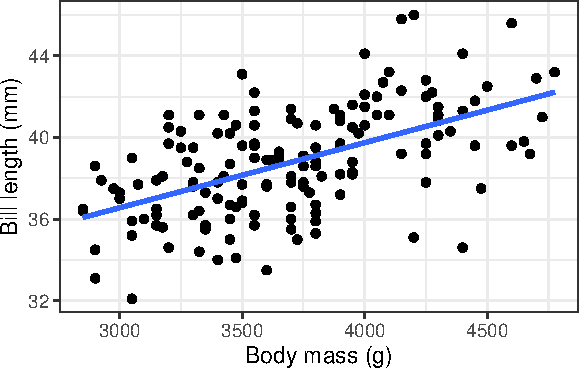
\includegraphics[width=0.6\linewidth,height=\textheight,keepaspectratio]{index_files/mediabag/simple_linear_regression_files/figure-pdf/fig-lm-1.pdf}

}

\caption{\label{fig-lm}Scatter plot of the Palmer Station Adelie penguin
data with a best fit line.}

\end{figure}%

Although there is some scatter in the data (Figure~\ref{fig-lm}), there
appears to be a positive relationship between the body mass and bill
length of the penguins. This relationship might be amenable for
modelling with a linear relationship and we shall continue to explore
this.

\subsection{State the Hypothesis}\label{state-the-hypothesis}

\begin{itemize}
\tightlist
\item
  Null Hypothesis (\(H_0\)): there is no relationship between the body
  mass of the penguins and their bill length.
\item
  Alternative Hypothesis (\(H_A\)): there is a relationship between the
  two variables.
\end{itemize}

This can be written as:

\begin{equation}\phantomsection\label{eq-h0}{H_{0}:\beta = 0}\end{equation}

As seen above, this hypothesis concerns the slope of the regression
line, \(\beta\). If the slope is zero, then there is no relationship
between the two variables. Regression models also tests an hypothesis
about the intercept, \(\alpha\), but this is less commonly reported.

\subsection{Fit the Model}\label{sec-fit-model}

Since the assumptions of a linear regression can only be tested
\emph{after} fitting the model, we first fit the model and then test the
assumptions.

\begin{Shaded}
\begin{Highlighting}[]
\NormalTok{mod1 }\OtherTok{\textless{}{-}} \FunctionTok{lm}\NormalTok{(bill\_length\_mm }\SpecialCharTok{\textasciitilde{}}\NormalTok{ body\_mass\_g,}
           \AttributeTok{data =}\NormalTok{ Adelie)}
\FunctionTok{summary}\NormalTok{(mod1)}
\SpecialCharTok{\textgreater{}} 
\ErrorTok{\textgreater{}}\NormalTok{ Call}\SpecialCharTok{:}
\ErrorTok{\textgreater{}} \FunctionTok{lm}\NormalTok{(}\AttributeTok{formula =}\NormalTok{ bill\_length\_mm }\SpecialCharTok{\textasciitilde{}}\NormalTok{ body\_mass\_g, }\AttributeTok{data =}\NormalTok{ Adelie)}
\SpecialCharTok{\textgreater{}} 
\ErrorTok{\textgreater{}}\NormalTok{ Residuals}\SpecialCharTok{:}
\ErrorTok{\textgreater{}}\NormalTok{     Min      }\DecValTok{1}\NormalTok{Q  Median      }\DecValTok{3}\NormalTok{Q     Max }
\SpecialCharTok{\textgreater{}} \SpecialCharTok{{-}}\FloatTok{6.4208} \SpecialCharTok{{-}}\FloatTok{1.3690}  \FloatTok{0.1874}  \FloatTok{1.4825}  \FloatTok{5.6168} 
\SpecialCharTok{\textgreater{}} 
\ErrorTok{\textgreater{}}\NormalTok{ Coefficients}\SpecialCharTok{:}
\ErrorTok{\textgreater{}}\NormalTok{              Estimate Std. Error t value }\FunctionTok{Pr}\NormalTok{(}\SpecialCharTok{\textgreater{}}\ErrorTok{|}\NormalTok{t}\SpecialCharTok{|}\NormalTok{)    }
\SpecialCharTok{\textgreater{}}\NormalTok{ (Intercept) }\FloatTok{2.699e+01}  \FloatTok{1.483e+00}  \FloatTok{18.201}  \SpecialCharTok{\textless{}} \FloatTok{2e{-}16} \SpecialCharTok{**}\ErrorTok{*}
\ErrorTok{\textgreater{}}\NormalTok{ body\_mass\_g }\FloatTok{3.188e{-}03}  \FloatTok{3.977e{-}04}   \FloatTok{8.015} \FloatTok{2.95e{-}13} \SpecialCharTok{**}\ErrorTok{*}
\ErrorTok{\textgreater{}} \SpecialCharTok{{-}{-}{-}}
\ErrorTok{\textgreater{}}\NormalTok{ Signif. codes}\SpecialCharTok{:}  \DecValTok{0} \StringTok{\textquotesingle{}***\textquotesingle{}} \FloatTok{0.001} \StringTok{\textquotesingle{}**\textquotesingle{}} \FloatTok{0.01} \StringTok{\textquotesingle{}*\textquotesingle{}} \FloatTok{0.05} \StringTok{\textquotesingle{}.\textquotesingle{}} \FloatTok{0.1} \StringTok{\textquotesingle{} \textquotesingle{}} \DecValTok{1}
\SpecialCharTok{\textgreater{}} 
\ErrorTok{\textgreater{}}\NormalTok{ Residual standard error}\SpecialCharTok{:} \FloatTok{2.234}\NormalTok{ on }\DecValTok{149}\NormalTok{ degrees of freedom}
\SpecialCharTok{\textgreater{}}\NormalTok{ Multiple R}\SpecialCharTok{{-}}\NormalTok{squared}\SpecialCharTok{:}  \FloatTok{0.3013}\NormalTok{,  Adjusted R}\SpecialCharTok{{-}}\NormalTok{squared}\SpecialCharTok{:}  \FloatTok{0.2966} 
\SpecialCharTok{\textgreater{}}\NormalTok{ F}\SpecialCharTok{{-}}\NormalTok{statistic}\SpecialCharTok{:} \FloatTok{64.24}\NormalTok{ on }\DecValTok{1}\NormalTok{ and }\DecValTok{149}\NormalTok{ DF,  p}\SpecialCharTok{{-}}\NormalTok{value}\SpecialCharTok{:} \FloatTok{2.955e{-}13}
\end{Highlighting}
\end{Shaded}

\subsection{Test the Assumptions}\label{test-the-assumptions}

Assumptions of normality, homoscedasticity, and linearity must be tested
(Section~\ref{sec-assumptions}).

We already noted that a linear model will probably be appropriate for
the data (see Figure~\ref{fig-lm}), so we proceed with the other
assumptions.

To facilitate the production of the diagnostic plots, we will use the
\textbf{broom} package's \texttt{augment()} function to add the
residuals to the data within the original dataset (now appearing as the
tidied dataset, \texttt{mod1\_data}). This will allow us to create the
diagnostic plots more easily, and later we can also use it to look for
the presence of outliers (Section~\ref{sec-outlier-test}).

\begin{Shaded}
\begin{Highlighting}[]
\FunctionTok{library}\NormalTok{(broom)}

\NormalTok{mod1\_data }\OtherTok{\textless{}{-}} \FunctionTok{augment}\NormalTok{(mod1)}
\end{Highlighting}
\end{Shaded}

\textbf{Normality}

I first check the normality assumption using one of several options
(Options 1-3). Here I use the Shapiro-Wilk test, a Residual Q-Q plot,
and a histogram of the residuals.

\textbf{Option 1}: Perform the Shapiro-Wilk test on the residuals. The
Shapiro-Wilk test is useful for detecting departures from normality in
small sample sizes. The hypothesis is:

\begin{itemize}
\tightlist
\item
  H\textsubscript{0}: the residuals are normally distributed.
\item
  H\textsubscript{A}: the residuals are not normally distributed.
\end{itemize}

\begin{Shaded}
\begin{Highlighting}[]
\FunctionTok{shapiro.test}\NormalTok{(}\FunctionTok{residuals}\NormalTok{(mod1))}
\SpecialCharTok{\textgreater{}} 
\ErrorTok{\textgreater{}}\NormalTok{   Shapiro}\SpecialCharTok{{-}}\NormalTok{Wilk normality test}
\SpecialCharTok{\textgreater{}} 
\ErrorTok{\textgreater{}}\NormalTok{ data}\SpecialCharTok{:}  \FunctionTok{residuals}\NormalTok{(mod1)}
\SpecialCharTok{\textgreater{}}\NormalTok{ W }\OtherTok{=} \FloatTok{0.99613}\NormalTok{, p}\SpecialCharTok{{-}}\NormalTok{value }\OtherTok{=} \FloatTok{0.9637}
\end{Highlighting}
\end{Shaded}

The \emph{p}-value is greater than 0.05, so I reject the alternative
hypothesis. I conclude that the residuals are normally distributed.

\textbf{Option 2}: Create a Residual Q-Q plot to visually assess the
normality of the residuals:

\begin{figure}[tbp]

\centering{

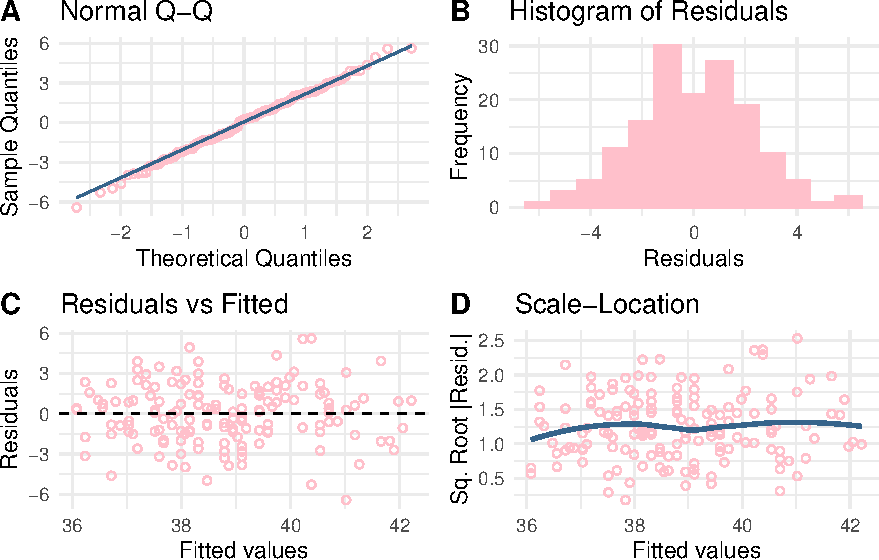
\includegraphics[width=0.8\linewidth,height=\textheight,keepaspectratio]{index_files/mediabag/simple_linear_regression_files/figure-pdf/fig-assump-plots-1.pdf}

}

\caption{\label{fig-assump-plots}Diagnostics plots the linear
regression, \texttt{mod1}, for assumption testing.}

\end{figure}%

The residuals are plotted against a theoretical normal distribution. The
residuals fall along the line without major deviations, therefore the
residuals are normally distributed (Figure~\ref{fig-assump-plots} A).

\textbf{Option 3}: Create a histogram of the residuals to visually
assess the normality of the residuals:

The histogram of the residuals appears to be normally distributed
(Figure~\ref{fig-assump-plots} B).

\textbf{Homoscedasticity}

I now examine the homoscedasticity assumption. The residuals should be
approximately equal across all values of the independent variable. There
are several options.

\textbf{Option 1}: I will use the Breusch-Pagan test to test for
homoscedasticity.

The Breusch-Pagan test is used to assess the presence of
heteroscedasticity (non-constant variance) in the residuals of a
regression model.

The hypothesis is:

\begin{itemize}
\tightlist
\item
  H\textsubscript{0}: the residuals are homoscedastic.
\item
  H\textsubscript{A}: the residuals are heteroscedastic.
\end{itemize}

\begin{Shaded}
\begin{Highlighting}[]
\FunctionTok{library}\NormalTok{(lmtest)}
\FunctionTok{bptest}\NormalTok{(mod1)}
\SpecialCharTok{\textgreater{}} 
\ErrorTok{\textgreater{}}\NormalTok{   studentized Breusch}\SpecialCharTok{{-}}\NormalTok{Pagan test}
\SpecialCharTok{\textgreater{}} 
\ErrorTok{\textgreater{}}\NormalTok{ data}\SpecialCharTok{:}\NormalTok{  mod1}
\SpecialCharTok{\textgreater{}}\NormalTok{ BP }\OtherTok{=} \FloatTok{1.6677}\NormalTok{, df }\OtherTok{=} \DecValTok{1}\NormalTok{, p}\SpecialCharTok{{-}}\NormalTok{value }\OtherTok{=} \FloatTok{0.1966}
\end{Highlighting}
\end{Shaded}

The \emph{p}-value is greater than 0.05, so I reject the alternative
hypothesis. I conclude that the residuals are homoscedastic.

\textbf{Option 2}: Create a plot of the residuals against the fitted
values to visually assess homoscedasticity:

The residuals are scattered evenly around zero from short through to
long bill lengths, indicating that the residuals have constant variance
(Figure~\ref{fig-assump-plots} C).

\textbf{Option 3}: Create a plot of the standardised residuals against
the independent variable to visually assess homoscedasticity:

The residuals are scattered evenly around zero from low through to high
bill lenghts, indicating that the residuals have constant variance
(Figure~\ref{fig-assump-plots} D).

Other tests for homoscedasticity include the Goldfeld-Quandt
(\texttt{lmtest::gqtest}) test, Levene's test
(\texttt{car::leveneTest}), and others.

\subsection{Check for outliers}\label{sec-outlier-test}

How do we identify outliers in linear regression analysis? There are
several approaches (see Figure~\ref{fig-lm2-outliers1}):

\begin{enumerate}
\def\labelenumi{\arabic{enumi}.}
\item
  \textbf{Difference in Fits (DFFITS):} DFFITS is a measure of the
  impact of each observation on the predicted values (fitted values) of
  the model. It quantifies how much the predicted values would change if
  an observation were removed from the analysis. DFFITS values
  \textgreater{} \(\text{Threshold} = 2 \sqrt{\frac{p}{n}}\) indicate
  observations that have a substantial impact on the predicted values
  and may be influential or outliers. Here, \(p\) is the number of
  parameters in the model (including the intercept, i.e.~2 in a simple
  linear regression) and \(n\) is the number of observations.
\item
  \textbf{Cook's Distance Plot:} Cook's distance is a measure of the
  influence of each observation on the estimated regression
  coefficients. The Cook's distance plot shows the Cook's distance
  values for each observation against the row numbers (or observation
  numbers). Points with large Cook's distance values (typically greater
  than \(\frac{4}{n}\)) indicate observations that are potentially
  influential and may have a significant impact on the regression
  results.
\item
  \textbf{Residuals vs Leverage Plot:} This plot displays the
  standardised residuals against the leverage values (hat values) for
  each observation. Leverage values measure the influence of an
  observation on the fitted values (predicted values) of the model. The
  plot helps identify outliers and influential observations. Points with
  high leverage (typically greater than 2-3 times the average leverage)
  and large residuals are considered influential observations that may
  warrant further investigation or potential removal from the analysis.
\item
  \textbf{Cook's Distance vs Lev./(1-Lev.) Plot:} This plot combines
  information from Cook's distance and leverage values. The
  \emph{x}-axis represents the leverage values divided by (1 minus the
  leverage values), which is a transformation that spreads out the
  points for better visualisation. The \emph{y}-axis shows the Cook's
  distance values. This plot helps identify influential observations by
  considering both their impact on the regression coefficients (Cook's
  distance) and their influence on the fitted values (leverage). Points
  in the top-right corner of the plot indicate observations that are
  potentially influential and may require further examination or
  removal.
\end{enumerate}

\phantomsection\label{annotated-cell-11}%
\begin{Shaded}
\begin{Highlighting}[]
\NormalTok{cooksd\_thresh }\OtherTok{\textless{}{-}} \DecValTok{4} \SpecialCharTok{/} \FunctionTok{nrow}\NormalTok{(mod1\_data) }\hspace*{\fill}\NormalTok{\circled{1}}
\NormalTok{dffits\_threshold }\OtherTok{\textless{}{-}} \DecValTok{2} \SpecialCharTok{*} \FunctionTok{sqrt}\NormalTok{(}\DecValTok{2} \SpecialCharTok{/} \FunctionTok{nrow}\NormalTok{(Adelie)) }\hspace*{\fill}\NormalTok{\circled{2}}

\NormalTok{mod1\_data }\OtherTok{\textless{}{-}}\NormalTok{ mod1\_data }\SpecialCharTok{\%\textgreater{}\%}
  \FunctionTok{mutate}\NormalTok{(}\AttributeTok{index =} \FunctionTok{row\_number}\NormalTok{(),}
         \AttributeTok{leverage =} \FunctionTok{hatvalues}\NormalTok{(mod1),}
         \AttributeTok{dffits =} \FunctionTok{dffits}\NormalTok{(mod1),}
         \AttributeTok{colour =} \FunctionTok{ifelse}\NormalTok{(.cooksd }\SpecialCharTok{\textgreater{}}\NormalTok{ cooksd\_thresh, }\StringTok{"black"}\NormalTok{, }\StringTok{"pink"}\NormalTok{))}
\end{Highlighting}
\end{Shaded}

\begin{description}
\tightlist
\item[\circled{1}]
Calculate thresholds for Cook's distance.
\item[\circled{2}]
Calculate the threshold for DFFITS.
\end{description}

\begin{figure}[h]

\centering{

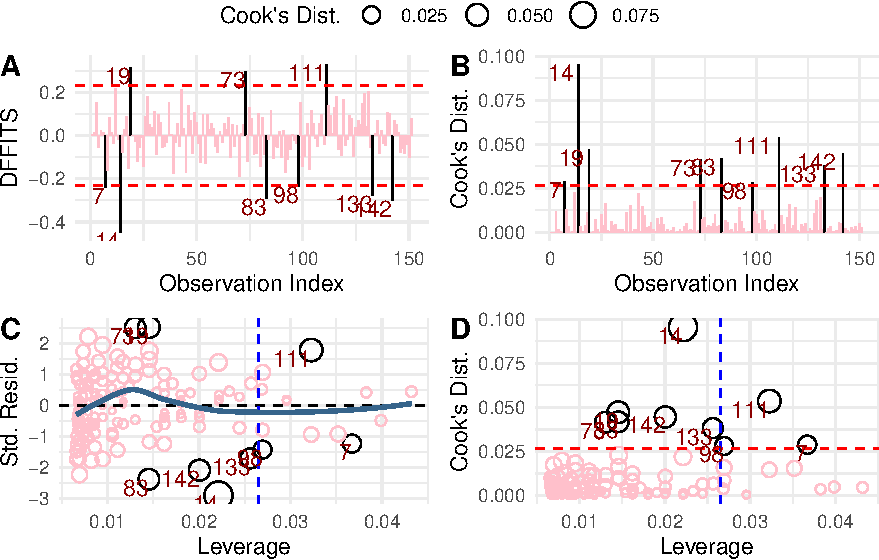
\includegraphics[width=0.8\linewidth,height=\textheight,keepaspectratio]{index_files/mediabag/simple_linear_regression_files/figure-pdf/fig-lm2-outliers1-1.pdf}

}

\caption{\label{fig-lm2-outliers1}Diagnostic plots for visual inspection
of outliers in the pernguin data. A) Difference in Fits (DFFITS) for
\texttt{mod1}. B) Cook's distance. C) Residuals vs.~leverage. D) Cook's
distance vs.~Lev./(1-Lev.). Outliers are identified beyond the Cook's
distance threshold (4/\emph{n}) and are plotted in black and their row
numbers in dark red. The vertical dashed blue lines in C) and D) are
positioned at 2 times the average leverage. The horizontal red dashed
lines in B) and D) are located at the Cook's distance threshold. A) to
C) are custom \textbf{ggplot2} plots corresponding to
\texttt{plot(mod1,\ which\ =\ c(4,\ 5,\ 6))}.}

\end{figure}%

\begin{figure}[tbp]

\centering{

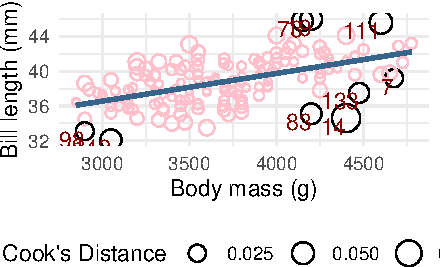
\includegraphics[width=0.4\linewidth,height=\textheight,keepaspectratio]{index_files/mediabag/simple_linear_regression_files/figure-pdf/fig-lm2-outliers2-1.pdf}

}

\caption{\label{fig-lm2-outliers2}Plot of the linear regression
resulting from \texttt{mod1} with the outliers identified using Cook's
distance highlighted.}

\end{figure}%

Once we have found them (Figure~\ref{fig-lm2-outliers2}), what do we do
with outliers? There are a few strategies:

\begin{enumerate}
\def\labelenumi{\arabic{enumi}.}
\item
  \textbf{Remove them:} If the outliers are due to data entry errors or
  other issues, it may be appropriate to remove them from the analysis.
  However, this should be done with caution, as outliers may be
  functionally important in the dataset if they represent rare, extreme
  events.
\item
  \textbf{Robust regression methods:} When there is certainty that the
  outliers are part of the observed response and represent extreme but
  rare occurrences, robust regression techniques such as M-estimation or
  least trimmed squares, which are less sensitive to the presence of
  outliers, could be used.
\item
  \textbf{Transformation of variables:} Applying appropriate
  transformations (e.g., logarithmic, square root) to the variables can
  sometimes reduce the impact of outliers.
\end{enumerate}

\subsection{Interpret the Results}\label{interpret-the-results}

Now that we have tested the assumptions, we can interpret the results of
the model fitted in Section~\ref{sec-fit-model}. The slope of the
regression line is 0.003188 mm/g, with a standard error of \(\pm\)
0.0003977. The \emph{p}-value is less than 0.001, so we reject the null
hypothesis that the slope is zero. We conclude that there is a
significant relationship between the body mass of the penguins and their
bill length.

The fit of the model is given by the multiple \(R^2\) value, which is
0.3013. This means that 30.13\% of the variation in bill length can be
explained by body mass. The remaining \textasciitilde70\% is due to
other factors not included in the model. The intercept of the model is
26.99 mm, with a standard error of \(\pm\) 0.0003977. The intercept is
the value of the dependent variable when the independent variable is
zero. In this case, it is the bill length of a penguin with a body mass
of zero grams, which is not a meaningful value.

The significance of the overall fit of the model can be assessed using
an analysis of variance (ANOVA) test. The \emph{p}-value is less than
0.001, so we reject the null hypothesis that the model does not explain
a significant amount of the variation in the data against an
\emph{F}-value of 64.25 on 1 and 149 degrees of freedom. We conclude
that the model is a good fit for the data.

\subsection{Reporting}\label{reporting}

I provide example Methods, Results, and Discussion sections in a format
more-or-less suited for inclusion in a scientific manuscript. Feel free
to use it as a template and edit it as necessary to describe your study.

\textbf{Methods}

\emph{Study data}

The data analysed in this study were derived from the Palmer Penguins
dataset, a comprehensive collection of measurements from three penguin
species (Adelie, Chinstrap, and Gentoo) collected in the Palmer
Archipelago, Antarctica. The dataset includes variables species, island,
bill length, bill depth, flipper length, body mass, and sex of the
penguins. This dataset has been made publicly available by Dr.~Kristen
Gorman and the Palmer Station, Antarctica LTER, a member of the Long
Term Ecological Research Network.

\emph{Statistical analysis}

The primary objective of our statistical analysis was to investigate the
relationship between the penguins' body mass and bill length. For this
purpose, we employed a simple linear regression model to quantify the
extent to which the independent variable predicts bill length.

We fitted a simple linear regression model using the \texttt{lm()}
function in R version 4.4.0 (R Core Team, 2024). The model included bill
length as the dependent variable, and body mass as continuous predictor.
We ensured all assumptions for linear regression were assessed including
linearity, independence, homoscedasticity, and normality of residuals.

After fitting the model, diagnostic plots were generated using the
\texttt{plot()} function in R to visually assess the residuals for any
patterns indicating potential violations of regression assumptions.
Additionally, the Shapiro-Wilk test was conducted to confirm the
normality of the residuals. The presence of heteroscedasticity was
evaluated using the Breusch-Pagan test.

The adequacy of the model fit was judged based on the coefficient of
determination (\emph{R}\textsuperscript{2}), which provided insight into
the variance in body mass explained by the predictors. The significance
of the regression coefficients was determined using \emph{t}-tests, and
the overall model fit was evaluated by an \emph{F}-test.

\textbf{Results}

\begin{figure}[t]

\centering{

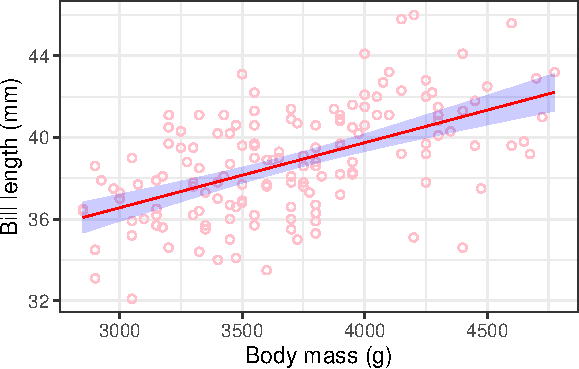
\includegraphics[width=0.6\linewidth,height=\textheight,keepaspectratio]{index_files/mediabag/simple_linear_regression_files/figure-pdf/fig-lm2-1.pdf}

}

\caption{\label{fig-lm2}Plot of bill length as a function of body mass
for Adelie penguins sampled at the Palmer Station. The straight line
indicates the best fit regression line and the blue shading is the 95\%
confidence interval.}

\end{figure}%

The regression coefficient for bill length with respect to body mass was
estimated to be approximately \(3.2 \times 10^{-3}\) mm/g \(\pm\)
\(3.977 \times 10^{-4}\) (mean slope \(\pm\) SE) (\(p < 0.001\),
\(t = 8.015\)), indicating a significant dependence of bill length on
body mass (Figure~\ref{fig-lm2}).

The multiple \(R^2\) value of the model was 0.3013, suggesting that
approximately 30.13\% of the variability in bill length can be accounted
for by changes in body mass. This indicates that while bill length
variation is notably influenced by body mass, about 69.87\% of the
variation is attributable to other factors not included in the model.

The overall fit of the model, assessed by an ANOVA, strongly supported
the model's validity (\(F = 64.25\), \(p < 0.001\), d.f. = \(1, 149\))
and confirms that a linear model provides adequate support for
predicting penguin bill length from body mass.

\textbf{Discussion}

In conclusion, the statistical analysis confirms a significant
relationship between body mass and bill length in penguins. Although the
model explains a substantial portion of the variation, future studies
should consider additional variables that could account for the
remaining variability in bill length. This would enhance our
understanding of the morphological adaptations of penguins in their
natural habitat.

\section{Confidence and Prediction
Intervals}\label{confidence-and-prediction-intervals}

Confidence intervals estimate the range within which the true mean of
the dependent variable (\(Y\)) is likely to fall for a given value of
the independent variable (\(X\)). In other words, if you were to repeat
your experiment many times and calculate the mean response at a specific
\(X\) value each time, the confidence interval would contain the true
population mean a certain percentage of the time (e.g., 95\%).
Therefore, a 95\% confidence interval means you can be 95\% confident
that the interval contains the true mean response for the population at
that particular \(X\) value. It's about the average, not individual data
points.

Prediction intervals, on the other hand, provide a range of \(Y\) values
that are likely to contain a single new observation of the dependent
variable for a given value of the independent variable \(X\). These
intervals account for the variability around individual observations and
are generally wider than confidence intervals because they include both
the variability of the estimated mean response and the variability of
individual observations around that mean. Continuing with the Adelie
penguin data, the confidence and prediction intervals are shown in
Figure~\ref{fig-lm2-conf}.

\begin{Shaded}
\begin{Highlighting}[]
\CommentTok{\# Predict values with confidence intervals}
\NormalTok{pred\_conf }\OtherTok{\textless{}{-}} \FunctionTok{as.data.frame}\NormalTok{(}\FunctionTok{predict}\NormalTok{(mod1,}
                                   \AttributeTok{newdata =}\NormalTok{ Adelie,}
                                   \AttributeTok{interval =} \StringTok{"confidence"}\NormalTok{))}

\CommentTok{\# Predict values with prediction intervals}
\NormalTok{pred\_pred }\OtherTok{\textless{}{-}} \FunctionTok{as.data.frame}\NormalTok{(}\FunctionTok{predict}\NormalTok{(mod1,}
                                   \AttributeTok{newdata =}\NormalTok{ Adelie,}
                                   \AttributeTok{interval =} \StringTok{"prediction"}\NormalTok{))}

\CommentTok{\# Add body mass to the data frame}
\NormalTok{results }\OtherTok{\textless{}{-}} \FunctionTok{cbind}\NormalTok{(Adelie, pred\_conf, pred\_pred[,}\DecValTok{2}\SpecialCharTok{:}\DecValTok{3}\NormalTok{])}

\CommentTok{\# Rename columns for clarity}
\FunctionTok{names}\NormalTok{(results)[}\FunctionTok{c}\NormalTok{(}\DecValTok{9}\SpecialCharTok{:}\DecValTok{13}\NormalTok{)] }\OtherTok{\textless{}{-}} \FunctionTok{c}\NormalTok{(}\StringTok{"fit"}\NormalTok{, }\StringTok{"lwr\_conf"}\NormalTok{, }\StringTok{"upr\_conf"}\NormalTok{,}
                             \StringTok{"lwr\_pred"}\NormalTok{, }\StringTok{"upr\_pred"}\NormalTok{)}

\FunctionTok{ggplot}\NormalTok{(}\AttributeTok{data =}\NormalTok{ results, }\FunctionTok{aes}\NormalTok{(}\AttributeTok{x =}\NormalTok{ body\_mass\_g, }\AttributeTok{y =}\NormalTok{ fit)) }\SpecialCharTok{+}
  \FunctionTok{geom\_line}\NormalTok{(}\AttributeTok{linewidth =} \FloatTok{0.4}\NormalTok{, }\AttributeTok{colour =} \StringTok{"red"}\NormalTok{) }\SpecialCharTok{+}
  \FunctionTok{geom\_ribbon}\NormalTok{(}\FunctionTok{aes}\NormalTok{(}\AttributeTok{ymin =}\NormalTok{ lwr\_pred, }\AttributeTok{ymax =}\NormalTok{ upr\_pred),}
              \AttributeTok{alpha =} \FloatTok{0.2}\NormalTok{, }\AttributeTok{fill =} \StringTok{"red"}\NormalTok{) }\SpecialCharTok{+}
  \FunctionTok{geom\_ribbon}\NormalTok{(}\FunctionTok{aes}\NormalTok{(}\AttributeTok{ymin =}\NormalTok{ lwr\_conf, }\AttributeTok{ymax =}\NormalTok{ upr\_conf),}
              \AttributeTok{alpha =} \FloatTok{0.2}\NormalTok{, }\AttributeTok{fill =} \StringTok{"blue"}\NormalTok{) }\SpecialCharTok{+}
  \FunctionTok{geom\_point}\NormalTok{(}\FunctionTok{aes}\NormalTok{(}\AttributeTok{y =}\NormalTok{ bill\_length\_mm), }\AttributeTok{shape =} \DecValTok{1}\NormalTok{) }\SpecialCharTok{+}
  \FunctionTok{labs}\NormalTok{(}\AttributeTok{x =} \StringTok{"Body mass (g)"}\NormalTok{, }\AttributeTok{y =} \StringTok{"Bill length (mm)"}\NormalTok{) }\SpecialCharTok{+}
  \FunctionTok{theme\_bw}\NormalTok{()}
\end{Highlighting}
\end{Shaded}

\begin{figure}[t]

\centering{

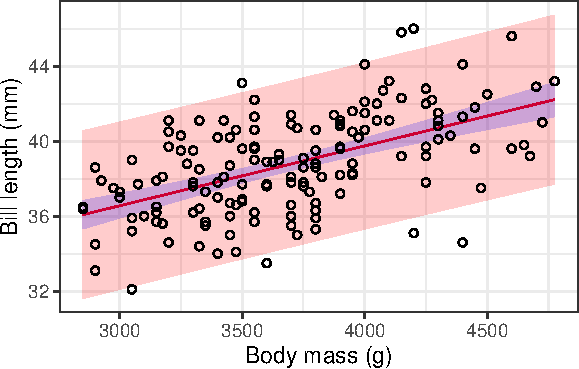
\includegraphics[width=0.6\linewidth,height=\textheight,keepaspectratio]{index_files/mediabag/simple_linear_regression_files/figure-pdf/fig-lm2-conf-1.pdf}

}

\caption{\label{fig-lm2-conf}Plot of pernguin data with the confidence
interval (blue) and prediction interval (pink) around the fitted
values.}

\end{figure}%

Confidence and prediction intervals are relevant for understanding the
uncertainty associated with a linear regression model's predictions.
While confidence intervals focus on quantifying the uncertainty around
the estimated mean response, prediction intervals comprehensively assess
the variability that can be expected for individual observations. We can
use both when interpreting the results of a linear regression analysis.

Confidence intervals are useful when the primary interest lies in making
inferences about the mean response at specific values of the independent
variable(s). For instance, in a study examining the relationship between
soil nutrient levels and plant biomass, confidence intervals can help
determine the range of mean biomass that can be expected for a given
level of soil nutrients. This information may be valuable for crop
management practices, such as designing fertilisation strategies or
assessing the impact of nutrient depletion on plant productivity.

Prediction intervals, on the other hand, are more relevant when the goal
is to predict the value of an individual observation or to assess the
range of values that future observations might take. For example, in a
study investigating the relationship between ambient temperature and the
growth rate of a species of fish, prediction intervals provide a range
of growth rates that an individual fish might exhibit based on the
observed temperature. This information is invaluable in aquaculture, for
instance, where predicting individual growth patterns can inform
decisions about optimal stocking densities or feed management
strategies.

The relative widths of confidence and prediction intervals can provide
insights into the variability in the data. If the prediction intervals
are substantially wider than the confidence intervals, it may indicate a
high level of variability in individual observations around the mean
response, which could suggest the presence of influential factors or
sources of variation that are not accounted for by the current model,
such as microhabitat differences or genetic variation within the studied
population.

\section{What Do I Do When Some Assumptions
Fail?}\label{sec-assumption-fails}

\subsection{Failing Assumptions of Normality and
Homoscedasticity}\label{sec-assumption-fails2}

I will use the sparrow data from Zar (1999) to demonstrate what to do
when the assumptions of normality and homoscedasticity are violated. I
will fit a linear model to the data and then check the assumptions.

\begin{figure}[t]

\centering{

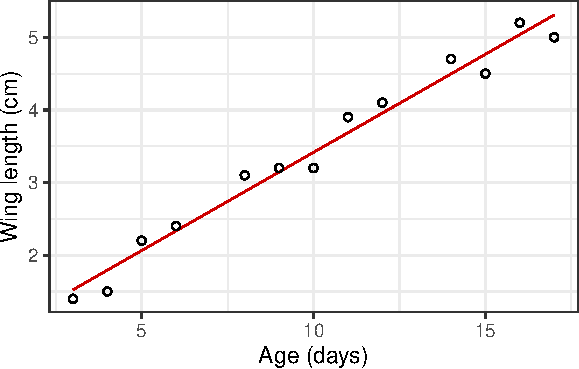
\includegraphics[width=0.6\linewidth,height=\textheight,keepaspectratio]{index_files/mediabag/simple_linear_regression_files/figure-pdf/fig-lm3-1.pdf}

}

\caption{\label{fig-lm3}Scatter plot of the sparrow dataset with a best
fit line.}

\end{figure}%

Figure~\ref{fig-lm3} is a scatter plot of the sparrow data with a best
fit line. At first glance, the linear model seems to almost perfectly
describe the relationship of wing length on age. I will fit a linear
model to the data and then check the assumptions.

\begin{Shaded}
\begin{Highlighting}[]
\NormalTok{mod2 }\OtherTok{\textless{}{-}} \FunctionTok{lm}\NormalTok{(wing }\SpecialCharTok{\textasciitilde{}}\NormalTok{ age, }\AttributeTok{data =}\NormalTok{ sparrows)}
\FunctionTok{summary}\NormalTok{(mod2)}
\SpecialCharTok{\textgreater{}} 
\ErrorTok{\textgreater{}}\NormalTok{ Call}\SpecialCharTok{:}
\ErrorTok{\textgreater{}} \FunctionTok{lm}\NormalTok{(}\AttributeTok{formula =}\NormalTok{ wing }\SpecialCharTok{\textasciitilde{}}\NormalTok{ age, }\AttributeTok{data =}\NormalTok{ sparrows)}
\SpecialCharTok{\textgreater{}} 
\ErrorTok{\textgreater{}}\NormalTok{ Residuals}\SpecialCharTok{:}
\ErrorTok{\textgreater{}}\NormalTok{      Min       }\DecValTok{1}\NormalTok{Q   Median       }\DecValTok{3}\NormalTok{Q      Max }
\SpecialCharTok{\textgreater{}} \SpecialCharTok{{-}}\FloatTok{0.30699} \SpecialCharTok{{-}}\FloatTok{0.21538}  \FloatTok{0.06553}  \FloatTok{0.16324}  \FloatTok{0.22507} 
\SpecialCharTok{\textgreater{}} 
\ErrorTok{\textgreater{}}\NormalTok{ Coefficients}\SpecialCharTok{:}
\ErrorTok{\textgreater{}}\NormalTok{             Estimate Std. Error t value }\FunctionTok{Pr}\NormalTok{(}\SpecialCharTok{\textgreater{}}\ErrorTok{|}\NormalTok{t}\SpecialCharTok{|}\NormalTok{)    }
\SpecialCharTok{\textgreater{}}\NormalTok{ (Intercept)  }\FloatTok{0.71309}    \FloatTok{0.14790}   \FloatTok{4.821} \FloatTok{0.000535} \SpecialCharTok{**}\ErrorTok{*}
\ErrorTok{\textgreater{}}\NormalTok{ age          }\FloatTok{0.27023}    \FloatTok{0.01349}  \FloatTok{20.027} \FloatTok{5.27e{-}10} \SpecialCharTok{**}\ErrorTok{*}
\ErrorTok{\textgreater{}} \SpecialCharTok{{-}{-}{-}}
\ErrorTok{\textgreater{}}\NormalTok{ Signif. codes}\SpecialCharTok{:}  \DecValTok{0} \StringTok{\textquotesingle{}***\textquotesingle{}} \FloatTok{0.001} \StringTok{\textquotesingle{}**\textquotesingle{}} \FloatTok{0.01} \StringTok{\textquotesingle{}*\textquotesingle{}} \FloatTok{0.05} \StringTok{\textquotesingle{}.\textquotesingle{}} \FloatTok{0.1} \StringTok{\textquotesingle{} \textquotesingle{}} \DecValTok{1}
\SpecialCharTok{\textgreater{}} 
\ErrorTok{\textgreater{}}\NormalTok{ Residual standard error}\SpecialCharTok{:} \FloatTok{0.2184}\NormalTok{ on }\DecValTok{11}\NormalTok{ degrees of freedom}
\SpecialCharTok{\textgreater{}}\NormalTok{ Multiple R}\SpecialCharTok{{-}}\NormalTok{squared}\SpecialCharTok{:}  \FloatTok{0.9733}\NormalTok{,  Adjusted R}\SpecialCharTok{{-}}\NormalTok{squared}\SpecialCharTok{:}  \FloatTok{0.9709} 
\SpecialCharTok{\textgreater{}}\NormalTok{ F}\SpecialCharTok{{-}}\NormalTok{statistic}\SpecialCharTok{:} \FloatTok{401.1}\NormalTok{ on }\DecValTok{1}\NormalTok{ and }\DecValTok{11}\NormalTok{ DF,  p}\SpecialCharTok{{-}}\NormalTok{value}\SpecialCharTok{:} \FloatTok{5.267e{-}10}
\end{Highlighting}
\end{Shaded}

Check the assumption of normality of residuals using the Shapiro-Wilk
test, a histogram, and a residual Q-Q plot.

\begin{Shaded}
\begin{Highlighting}[]
\FunctionTok{shapiro.test}\NormalTok{(}\FunctionTok{residuals}\NormalTok{(mod2))}
\SpecialCharTok{\textgreater{}} 
\ErrorTok{\textgreater{}}\NormalTok{   Shapiro}\SpecialCharTok{{-}}\NormalTok{Wilk normality test}
\SpecialCharTok{\textgreater{}} 
\ErrorTok{\textgreater{}}\NormalTok{ data}\SpecialCharTok{:}  \FunctionTok{residuals}\NormalTok{(mod2)}
\SpecialCharTok{\textgreater{}}\NormalTok{ W }\OtherTok{=} \FloatTok{0.84542}\NormalTok{, p}\SpecialCharTok{{-}}\NormalTok{value }\OtherTok{=} \FloatTok{0.02487}
\end{Highlighting}
\end{Shaded}

The \emph{p}-value for the Shapiro-Wilk test is \textless{} 0.05,
indicating that the residuals are not normally distributed. The
histogram and Q-Q plot of the residuals also show that the residuals are
not normally distributed (Figure~\ref{fig-hist2} and
Figure~\ref{fig-QQ2}). In the Residual Q-Q plot, the points deviate from
the straight line, indicating non-normality---note the S-shaped
curvature to the data.

\begin{Shaded}
\begin{Highlighting}[]
\FunctionTok{hist}\NormalTok{(}\FunctionTok{residuals}\NormalTok{(mod2))}
\end{Highlighting}
\end{Shaded}

\begin{figure}[tbp]

\centering{

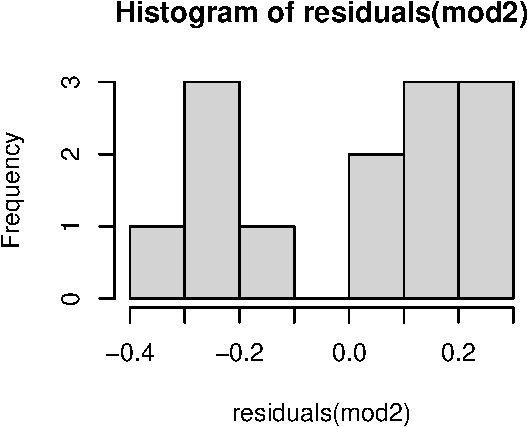
\includegraphics[width=0.6\linewidth,height=\textheight,keepaspectratio]{index_files/mediabag/simple_linear_regression_files/figure-pdf/fig-hist2-1.pdf}

}

\caption{\label{fig-hist2}A histogram of the residual of the linear
regression, \texttt{mod2}.}

\end{figure}%

\begin{Shaded}
\begin{Highlighting}[]
\FunctionTok{plot}\NormalTok{(mod2, }\AttributeTok{which =} \DecValTok{2}\NormalTok{)}
\end{Highlighting}
\end{Shaded}

\begin{figure}[tbp]

\centering{

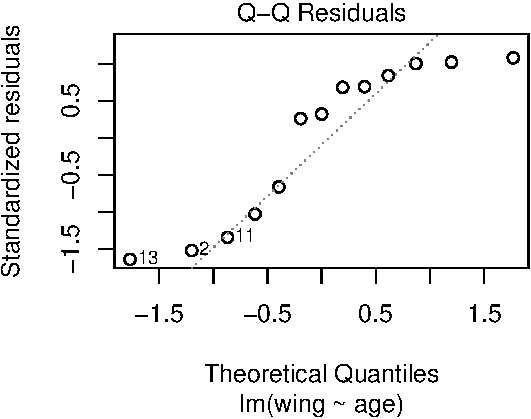
\includegraphics[width=0.6\linewidth,height=\textheight,keepaspectratio]{index_files/mediabag/simple_linear_regression_files/figure-pdf/fig-QQ2-1.pdf}

}

\caption{\label{fig-QQ2}A Residual Q-Q plot of the linear regression,
\texttt{mod2}.}

\end{figure}%

It is enough to know that the normality assumption is not met -- I
cannot proceed with a simple linear regression. However, let us for
completeness also look at the homoscedasticity assumption. I will use
the Breusch-Pagan test to check for homoscedasticity, followed by a plot
of residuals against fitted values.

\begin{Shaded}
\begin{Highlighting}[]
\FunctionTok{bptest}\NormalTok{(mod2)}
\SpecialCharTok{\textgreater{}} 
\ErrorTok{\textgreater{}}\NormalTok{   studentized Breusch}\SpecialCharTok{{-}}\NormalTok{Pagan test}
\SpecialCharTok{\textgreater{}} 
\ErrorTok{\textgreater{}}\NormalTok{ data}\SpecialCharTok{:}\NormalTok{  mod2}
\SpecialCharTok{\textgreater{}}\NormalTok{ BP }\OtherTok{=} \FloatTok{1.6349}\NormalTok{, df }\OtherTok{=} \DecValTok{1}\NormalTok{, p}\SpecialCharTok{{-}}\NormalTok{value }\OtherTok{=} \FloatTok{0.201}
\end{Highlighting}
\end{Shaded}

The \emph{p}-value for the Breusch-Pagan test is \textgreater{} 0.05,
indicating that the residuals are homoscedastic. The plot of residuals
against fitted values shows gives a slightly different impression
(Figure~\ref{fig-resid2}).

\begin{Shaded}
\begin{Highlighting}[]
\FunctionTok{plot}\NormalTok{(mod2, }\AttributeTok{which =} \DecValTok{1}\NormalTok{)}
\end{Highlighting}
\end{Shaded}

\begin{figure}[tbp]

\centering{

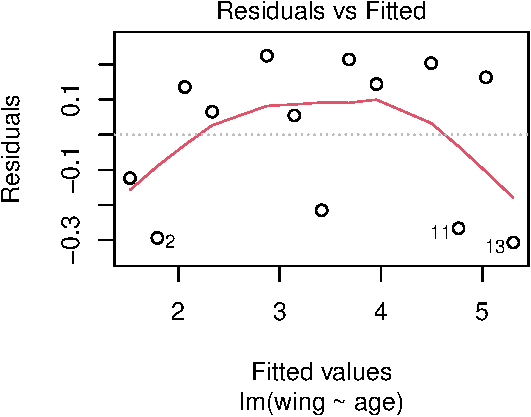
\includegraphics[width=0.6\linewidth,height=\textheight,keepaspectratio]{index_files/mediabag/simple_linear_regression_files/figure-pdf/fig-resid2-1.pdf}

}

\caption{\label{fig-resid2}A plot of residuals against fitted values for
the linear regression, \texttt{mod2}.}

\end{figure}%

The assumptions of normality and homoscedasticity are violated (it is
sufficient that one or the other fails, not both). As already noted, I
cannot proceed with the linear model. I will need to consider
alternative models or transformations to address these issues.

When the assumptions of normality and homoscedasticity are violated, I
have some options---these broadly group into transforming the data and
using a non-parametric test.

Transforming the data can sometimes help attain normality and
homoscedasticity. Common transformations include the logarithmic, square
root, and inverse transformations. However, be cautious when
interpreting the results of transformed data, as the transformed
coefficients may not be directly interpretable.

I will show the Theil-Sen estimator (also known as Sen's slope
estimator) as a robust non-parametric replacement for a simple linear
model. It calculates the median of the slopes of all pairs of sample
points to determine the overall slope of the line.

\begin{Shaded}
\begin{Highlighting}[]
\FunctionTok{library}\NormalTok{(mblm)}

\NormalTok{mod3 }\OtherTok{\textless{}{-}} \FunctionTok{mblm}\NormalTok{(wing }\SpecialCharTok{\textasciitilde{}}\NormalTok{ age, }\AttributeTok{data =}\NormalTok{ sparrows)}
\FunctionTok{summary}\NormalTok{(mod3)}
\SpecialCharTok{\textgreater{}} 
\ErrorTok{\textgreater{}}\NormalTok{ Call}\SpecialCharTok{:}
\ErrorTok{\textgreater{}} \FunctionTok{mblm}\NormalTok{(}\AttributeTok{formula =}\NormalTok{ wing }\SpecialCharTok{\textasciitilde{}}\NormalTok{ age, }\AttributeTok{dataframe =}\NormalTok{ sparrows)}
\SpecialCharTok{\textgreater{}} 
\ErrorTok{\textgreater{}}\NormalTok{ Residuals}\SpecialCharTok{:}
\ErrorTok{\textgreater{}}\NormalTok{      Min       }\DecValTok{1}\NormalTok{Q   Median       }\DecValTok{3}\NormalTok{Q      Max }
\SpecialCharTok{\textgreater{}} \SpecialCharTok{{-}}\FloatTok{0.44524} \SpecialCharTok{{-}}\FloatTok{0.31190} \SpecialCharTok{{-}}\FloatTok{0.00714}  \FloatTok{0.06905}  \FloatTok{0.14048} 
\SpecialCharTok{\textgreater{}} 
\ErrorTok{\textgreater{}}\NormalTok{ Coefficients}\SpecialCharTok{:}
\ErrorTok{\textgreater{}}\NormalTok{             Estimate     MAD V value }\FunctionTok{Pr}\NormalTok{(}\SpecialCharTok{\textgreater{}}\ErrorTok{|}\NormalTok{V}\SpecialCharTok{|}\NormalTok{)    }
\SpecialCharTok{\textgreater{}}\NormalTok{ (Intercept)  }\FloatTok{0.75000} \FloatTok{0.18532}      \DecValTok{91} \FloatTok{0.000244} \SpecialCharTok{**}\ErrorTok{*}
\ErrorTok{\textgreater{}}\NormalTok{ age          }\FloatTok{0.27619} \FloatTok{0.00956}      \DecValTok{91} \FloatTok{0.000244} \SpecialCharTok{**}\ErrorTok{*}
\ErrorTok{\textgreater{}} \SpecialCharTok{{-}{-}{-}}
\ErrorTok{\textgreater{}}\NormalTok{ Signif. codes}\SpecialCharTok{:}  \DecValTok{0} \StringTok{\textquotesingle{}***\textquotesingle{}} \FloatTok{0.001} \StringTok{\textquotesingle{}**\textquotesingle{}} \FloatTok{0.01} \StringTok{\textquotesingle{}*\textquotesingle{}} \FloatTok{0.05} \StringTok{\textquotesingle{}.\textquotesingle{}} \FloatTok{0.1} \StringTok{\textquotesingle{} \textquotesingle{}} \DecValTok{1}
\SpecialCharTok{\textgreater{}} 
\ErrorTok{\textgreater{}}\NormalTok{ Residual standard error}\SpecialCharTok{:} \FloatTok{0.244}\NormalTok{ on }\DecValTok{11}\NormalTok{ degrees of freedom}
\end{Highlighting}
\end{Shaded}

The interpretation of the Theil-Sen estimator is similar to the simple
linear regression. The Theil-Sen estimator provides a robust estimate of
the slope of the relationship between age and wing length. The slope of
the line is 0.28 (\(\pm\) 0.19 mean absolute deviation) (\emph{V} value
= 91, \emph{p} \textless{} 0.001), indicating that for each additional
day of age, the wing length increases by 0.28 cm. The intercept of the
line is 0.75, indicating that the wing length is \textasciitilde0.8 cm
when the age is 0 days.

\subsection{My Data Do Not Display a Linear
Response}\label{my-data-do-not-display-a-linear-response}

In simple linear regression, the dependent variable \(Y\) is expected to
exhibit a straight-line relationship with the independent variable
\(X\). However, several factors can cause deviations from a linear
pattern.

Statistical assumptions underlying linear regression can affect the
appearance of a linear response. The normality assumption is important
but primarily pertains to the residuals rather than the \(Y\) vs.~\(X\)
plot. A scatterplot of \(Y\) vs.~\(X\) might deviate from a linear
pattern due to the non-normality of the residuals or heteroscedasticity,
where the variability of the residuals changes with the level of \(X\).
Addressing these issues and then reassessing the linearity of the
relationship is a logical first step. Refer to
Section~\ref{sec-assumption-fails} for more details on how to proceed.

Outliers in the data can significantly impact the regression line,
leading to misleading results (Section~\ref{sec-outlier-test}).
Measurement errors in the independent variable can also lead to biased
and inconsistent estimations, which may require revisiting the data
collection process to address systemic problems. Variable bias, where
excluding relevant variables distorts the observed relationship, could
also explain seemingly nonlinear responses. Considering multiple
predictor variables in a regression model
(Chapter~\ref{sec-multiple-linear-regression}) might be more appropriate
in such situations.

It's important to note that simple linear regression might not be
suitable for all scenarios. For instance, the dependent variable \(Y\)
might inherently follow a different probability distribution, such as a
Poisson or a binomial distribution, rather than a normal distribution.
This is particularly relevant in count data or binary outcome scenarios.
In such cases, other types of models like Poisson regression or logistic
regression, accommodated by generalised linear models (GLM;
Chapter~\ref{sec-generalised-linear-model}), would be more appropriate.

Lastly, if the data do not exhibit a linear relationship even after
addressing these issues, the relationship between the variables may
really be nonlinear. This can occur when the underlying functional
relationship between \(X\) and \(Y\) is better described by exponential,
logarithmic, or other more complex mechanistic responses. In such cases,
nonlinear regression (Chapter~\ref{sec-nonlinear-regression}) or
generalised additive models (GAM;
Chapter~\ref{sec-generalised-additive-models}) might be necessary to
describe the relationship between the variables accurately.

\chapter{Polynomial Regression}\label{sec-polynomial-regression}

Polynomial regressions\index{polynomial regression} may resemble
non-linear regression in terms of the visual appearance of the
regression line (i.e.~with bends and curves), but they handle
non-linearity by transforming the independent variable \(X\) into higher
powers (e.g., \(X^2\), \(X^3\)), which are then included in the model
along with coefficients that are linear in terms of estimation. For
instance, a cubic (of \emph{order}, \emph{degree}, or \emph{power} 3;
denoted as \(m\)) polynomial regression model (Figure~\ref{fig-plts} A)
and is expressed as:

\begin{equation}\phantomsection\label{eq-poly}{Y_i = \alpha + \beta_1 X_i + \beta_2 X_i^2 + \beta_3 X_i^3 + \epsilon_i}\end{equation}

Where:

\begin{itemize}
\tightlist
\item
  \(Y_i\) is the response variable for the \(i\)-th observation,
\item
  \(X_i\) is the predictor variable for the \(i\)-th observation,
\item
  \(\alpha\) is the intercept,
\item
  \(\beta_1\), \(\beta_2\), and \(\beta_3\) are the coefficients for the
  linear, quadratic, and cubic terms, respectively, and
\item
  \(\epsilon_i\) is the error term for the \(i\)-th observation (the
  residuals).
\end{itemize}

It is worth noting that higher order polynomials can lead to
overfitting\index{overfitting}, where the model captures the noise in
the data rather than the inherent pattern. This can result in poor
generalisation to new data and poor predictive performance. Overfitting
becomes more likely as \(m\) increases. The \(m\) of a polynomial should
not exceed \(n-1\), where \(n\) is the number of data points. An \(m\)
greater than 4 or 5 is rarely justified.\footnote{The appropriate
  maximum \(m\) can be determined using methods such as the
  backward-elimination or forward-selection multiple-regression
  procedure.} If \(m=n-1\), the polynomial will fit the data perfectly
(i.e., \(R^2=1\)). For example, a linear regression (\(m=1\)) fits two
data points exactly, a quadratic regression (\(m = 2\)) fits three data
points perfectly, and so on. Therefore, always consider the trade-off
between model complexity and generalisation when using polynomial
regression.

Another complication is that the biological interpretation of more
complex (higher order) models may be lacking. However, polynomial
regression are more often than not used for prediction rather than their
interpretability.

\textless THE REST OF THIS CHAPTER IS TO BE DEVELOPED.\textgreater{}

\chapter{Multiple Linear
Regression}\label{sec-multiple-linear-regression}

In Section~\ref{sec-simple-linear-regression} we have seen how to model
the relationship between two variables using simple linear regression
(SLR). However, in ecosystems, the relationship between the response
variable and the explanatory variables is more complex and in many cases
cannot be adequately captured by a single driver (i.e.~influential or
predictor variable). In such cases, multiple linear regression (MLR) can
be used to model the relationship between the response variable and
multiple explanatory variables.

\section{Multiple Linear Regression}\label{multiple-linear-regression}

Multiple linear regression helps us answer questions such as:

\begin{itemize}
\tightlist
\item
  How do various environmental factors influence the population size of
  a species? Factors like average temperature, precipitation levels, and
  habitat area can be used to predict the population size of a species
  in a given region. Which of these factors are most important in
  determining the population size?
\item
  What are the determinants of plant growth in different ecosystems?
  Variables such as soil nutrient content, water availability, and light
  exposure can help predict the growth rate of plants in various
  ecosystems. How do these factors interact to influence plant growth?
\item
  How do genetic and environmental factors affect the spread of a
  disease in a population? The incidence of a disease might depend on
  factors like genetic susceptibility, exposure to pathogens, and
  environmental conditions (e.g., humidity and temperature). What is the
  relative importance of these factors in determining the spread of the
  disease?
\end{itemize}

Multiple linear regression extends the simple linear regression model to
include several independent variables. The model is expressed as:
\begin{equation}\phantomsection\label{eq-mlr1}{Y_i = \alpha + \beta_1 X_{i1} + \beta_2 X_{i2} + \ldots + \beta_k X_{ik} + \epsilon_i}\end{equation}
Where:

\begin{itemize}
\tightlist
\item
  \(Y_i\) is the response variable for the \(i\)-th observation,
\item
  \(X_{i1}, X_{i2}, \ldots, X_{ik}\) are the \(k\) predictor variables
  for the \(i\)-th observation,
\item
  \(\alpha\) is the intercept,
\item
  \(\beta_1, \beta_2, \ldots, \beta_k\) are the coefficients for the
  \(k\) predictor variables, and
\item
  \(\epsilon_i\) is the error term for the \(i\)-th observation (the
  residuals).
\end{itemize}

When including a categorical variable in a multiple linear regression
model, dummy (indicator) variables are used to represent the different
levels of the categorical variable. Let's assume we have a categorical
variable \(C\) with three levels: \(C_1\), \(C_2\), and \(C_3\). We can
represent this categorical variable using two dummy variables:

\begin{itemize}
\tightlist
\item
  \(D_1\): Equals 1 if \(C = C_2\), 0 otherwise.
\item
  \(D_2\): Equals 1 if \(C = C_3\), 0 otherwise.
\end{itemize}

\(C_1\) is considered the reference category and does not get a dummy
variable. This way, we avoid multicollinearity (see
Section~\ref{sec-multicollinearity}). R's \texttt{lm()} function will
automatically convert the categorical variables to dummy variables
(sometimes called treatment coding). The first level of the
alphabetically sorted categorical variable is taken as the reference
level. See Section~\ref{sec-r-function} for more information about how
to include categorical variables in a multiple linear regression model.
At the end of the chapter you'll find alternative ways to assess
categorical variables in a multiple linear regression model
(Section~\ref{sec-contrasts}).

Assume we also have \(k\) continuous predictors
\(X_{1}, X_{2}, \ldots, X_{k}\). The multiple linear regression model
with these predictors and the categorical variable can be expressed as:
\begin{equation}\phantomsection\label{eq-mlr2}{Y_i = \alpha + \beta_1 X_{i1} + \beta_2 X_{i2} + \ldots + \beta_k X_{ik} + \gamma_1 D_{i1} + \gamma_2 D_{i2} + \epsilon_i}\end{equation}
Where:

\begin{itemize}
\tightlist
\item
  \(Y_i\) is the dependent variable for observation \(i\).
\item
  \(\alpha\) is the intercept term.
\item
  \(\beta_1, \beta_2, \ldots, \beta_k\) are the coefficients for the
  continuous independent variables \(X_{i1}, X_{i2}, \ldots, X_{ik}\).
\item
  \(D_{i1}\) and \(D_{i2}\) are the dummy variables for the categorical
  predictor \(C\).
\item
  \(\gamma_1\) and \(\gamma_2\) are the coefficients for the dummy
  variables, representing the effect of levels \(C_2\) and \(C_3\)
  relative to the reference level \(C_1\).
\item
  \(\epsilon_i\) is the error term for observation \(i\).
\end{itemize}

\section{Nature of the Data}\label{nature-of-the-data-1}

You are referred to the discussion in simple linear regression
(Section~\ref{sec-simple-linear-regression}). The only added
consideration is that the data should be multivariate, i.e., it should
contain more than one predictor variable. The predictor variables are
generally continuous, but there may also be categorical variables.

\section{Assumptions}\label{assumptions}

Basically, this is as already discussed in simple linear regression
(Section~\ref{sec-simple-linear-regression})---in multiple linear
regression, the same assumptions apply to the response relative to each
of the predictor variables. In Section~\ref{sec-diagnostics} I will
assess the assumptions in an example dataset. An additional
consideration is that the predictors must not be highly correlated with
each other (multicollinearity) (see
Section~\ref{sec-multicollinearity}).

\section{Outliers}\label{outliers}

Again, this is as discussed in simple linear regression
(Section~\ref{sec-simple-linear-regression}). In multiple linear
regression, the same considerations apply to the response relative to
each of the predictor variables.

\section{R Function}\label{sec-r-function}

The \texttt{lm()} function in R is used to fit a multiple linear
regression model. The syntax is similar to that of the \texttt{lm()}
function used for simple linear regression, but with multiple predictor
variables. The function takes the basic form:

\begin{Shaded}
\begin{Highlighting}[]
\FunctionTok{lm}\NormalTok{(formula, data)}
\end{Highlighting}
\end{Shaded}

For a multiple linear regression with only continuous predictor
variables (as in Equation~\ref{eq-mlr1}), the formula is:

\begin{Shaded}
\begin{Highlighting}[]
\FunctionTok{lm}\NormalTok{(response }\SpecialCharTok{\textasciitilde{}}\NormalTok{ predictor1 }\SpecialCharTok{+}\NormalTok{ predictor2 }\SpecialCharTok{+}\NormalTok{ ... }\SpecialCharTok{+}\NormalTok{ predictorN,}
   \AttributeTok{data =}\NormalTok{ dataset)}
\end{Highlighting}
\end{Shaded}

Interaction effects are implemented by including the product of two
variables in the formula. For example, to include an interaction between
\texttt{predictor1} and \texttt{predictor2}, we can use:

\begin{Shaded}
\begin{Highlighting}[]
\FunctionTok{lm}\NormalTok{(response }\SpecialCharTok{\textasciitilde{}}\NormalTok{ predictor1 }\SpecialCharTok{*}\NormalTok{ predictor2, }\AttributeTok{data =}\NormalTok{ dataset)}
\end{Highlighting}
\end{Shaded}

When we have both continuous and categorical predictor variables
(Equation~\ref{eq-mlr2}), the formula is:

\begin{Shaded}
\begin{Highlighting}[]
\FunctionTok{lm}\NormalTok{(response }\SpecialCharTok{\textasciitilde{}}\NormalTok{ continuous\_predictor1 }\SpecialCharTok{+}\NormalTok{ continuous\_predictor2 }\SpecialCharTok{+}\NormalTok{ ...}
   \SpecialCharTok{+}\NormalTok{ continuous\_predictorN }\SpecialCharTok{+} \FunctionTok{factor}\NormalTok{(categorical\_predictor1) }\SpecialCharTok{+}
     \FunctionTok{factor}\NormalTok{(categorical\_predictor2) }\SpecialCharTok{+}\NormalTok{ ...}
   \SpecialCharTok{+} \FunctionTok{factor}\NormalTok{(categorical\_predictorM),}
   \AttributeTok{data =}\NormalTok{ dataset)}
\end{Highlighting}
\end{Shaded}

\section{Example 1: The Seaweed Dataset}\label{sec-example1}

Load some
\href{https://tangledbank.netlify.app/data/seaweed/spp_df2.csv}{data}
produced in the analysis by {[}3{]}. Please refer to the chapter
\href{https://tangledbank.netlify.app/BCB743/06-deep_dive.html}{Deep
Dive into Gradients} on Tangled Bank for the data description.

This dataset is suitable for a multiple linear regression because it has
continuous response variables (\(\beta_\text{sør}\),
\(\beta_\text{sim}\), and \(\beta_\text{sne}\), the Sørenesen
dissimilarity, the turnover component of \(\beta\)-diversity, and the
nestedness-resultant component of \(\beta\)-diversity, respectively),
continuous predictor variables (the mean climatological temperature for
August, the mean climatological temperature for the year, the
temperature range for February and August, and the SD of February and
August), and a categorical variable (the bioregional classification of
the samples).

\begin{Shaded}
\begin{Highlighting}[]
\NormalTok{sw }\OtherTok{\textless{}{-}} \FunctionTok{read.csv}\NormalTok{(}\StringTok{"data/spp\_df2.csv"}\NormalTok{)}
\FunctionTok{rbind}\NormalTok{(}\FunctionTok{head}\NormalTok{(sw, }\DecValTok{3}\NormalTok{), }\FunctionTok{tail}\NormalTok{(sw, }\DecValTok{3}\NormalTok{))[,}\SpecialCharTok{{-}}\DecValTok{1}\NormalTok{]}
\SpecialCharTok{\textgreater{}}\NormalTok{        dist  bio    augMean   febRange      febSD     augSD    annMean}
\SpecialCharTok{\textgreater{}} \DecValTok{1}     \FloatTok{0.000}\NormalTok{  BMP }\FloatTok{0.00000000} \FloatTok{0.00000000} \FloatTok{0.00000000} \FloatTok{0.0000000} \FloatTok{0.00000000}
\SpecialCharTok{\textgreater{}} \DecValTok{2}    \FloatTok{51.138}\NormalTok{  BMP }\FloatTok{0.05741369} \FloatTok{0.09884404} \FloatTok{0.16295271} \FloatTok{0.3132800} \FloatTok{0.01501846}
\SpecialCharTok{\textgreater{}} \DecValTok{3}   \FloatTok{104.443}\NormalTok{  BMP }\FloatTok{0.15043904} \FloatTok{0.34887754} \FloatTok{0.09934163} \FloatTok{0.4188239} \FloatTok{0.02602247}
\SpecialCharTok{\textgreater{}} \DecValTok{968} \FloatTok{102.649}\NormalTok{ ECTZ }\FloatTok{0.41496099} \FloatTok{0.11330069} \FloatTok{0.24304493} \FloatTok{0.7538546} \FloatTok{0.52278161}
\SpecialCharTok{\textgreater{}} \DecValTok{969}  \FloatTok{49.912}\NormalTok{ ECTZ }\FloatTok{0.17194242} \FloatTok{0.05756093} \FloatTok{0.18196664} \FloatTok{0.3604341} \FloatTok{0.24445006}
\SpecialCharTok{\textgreater{}} \DecValTok{970}   \FloatTok{0.000}\NormalTok{ ECTZ }\FloatTok{0.00000000} \FloatTok{0.00000000} \FloatTok{0.00000000} \FloatTok{0.0000000} \FloatTok{0.00000000}
\SpecialCharTok{\textgreater{}}\NormalTok{               Y        Y1          Y2}
\SpecialCharTok{\textgreater{}} \DecValTok{1}   \FloatTok{0.000000000} \FloatTok{0.0000000} \FloatTok{0.000000000}
\SpecialCharTok{\textgreater{}} \DecValTok{2}   \FloatTok{0.003610108} \FloatTok{0.0000000} \FloatTok{0.003610108}
\SpecialCharTok{\textgreater{}} \DecValTok{3}   \FloatTok{0.003610108} \FloatTok{0.0000000} \FloatTok{0.003610108}
\SpecialCharTok{\textgreater{}} \DecValTok{968} \FloatTok{0.198728140} \FloatTok{0.1948882} \FloatTok{0.003839961}
\SpecialCharTok{\textgreater{}} \DecValTok{969} \FloatTok{0.069337442} \FloatTok{0.0443038} \FloatTok{0.025033645}
\SpecialCharTok{\textgreater{}} \DecValTok{970} \FloatTok{0.000000000} \FloatTok{0.0000000} \FloatTok{0.000000000}
\end{Highlighting}
\end{Shaded}

We will do a multiple linear regression analysis to understand the
relationship between some of the environmental variables and the seaweed
species. Specifically, we will consider only the variables
\texttt{augMean}, \texttt{febRange}, \texttt{febSD}, \texttt{augSD}, and
\texttt{annMean} as predictors of the species composition as measured by
\(\beta_\text{sør}\) (\texttt{Y} in the data file).

The model, which we will call \texttt{full\_mod1} below, can be stated
formally as Equation~\ref{eq-full}:
\begin{equation}\phantomsection\label{eq-full}{Y = \alpha + \beta_1 X_1 + \beta_2 X_2 + \beta_3 X_3 + \beta_4 X_4 + \beta_5 X_5 + \epsilon}\end{equation}
Where:

\begin{itemize}
\tightlist
\item
  \(Y\) is the response variable, the mean Sørensen dissimilarity,
\item
  the predictors \(X_1\), \(X_2\), \(X_3\), \(X_4\), and \(X_5\)
  correspond to \texttt{augMean}, \texttt{febRange}, \texttt{febSD},
  \texttt{augSD}, and \texttt{annMean}, respectively, and
\item
  \(\epsilon\) is the error term.
\end{itemize}

But before we jump into multiple linear regression, let's warm up by
first fitting some simple linear regressions.

\subsection{Simple Linear Models}\label{simple-linear-models}

For interest sake, let's fit simple linear models for each of the
predictors against the response variable. Let's look at relationships
between the continuous predictors and the response in the East Coast
Transition Zone (\texttt{ECTZ}), ignoring the other bioregions for now.
We will first fit the simple linear models and then create scatter plots
of the response variable \(\beta_\text{sør}\) against each of the
predictor variables. To these plots, we will add a best fit (regression)
lines.

\begin{Shaded}
\begin{Highlighting}[]
\NormalTok{sw\_ectz }\OtherTok{\textless{}{-}}\NormalTok{ sw }\SpecialCharTok{|\textgreater{}} \FunctionTok{filter}\NormalTok{(bio }\SpecialCharTok{==} \StringTok{"ECTZ"}\NormalTok{)}

\NormalTok{predictors }\OtherTok{\textless{}{-}} \FunctionTok{c}\NormalTok{(}\StringTok{"augMean"}\NormalTok{, }\StringTok{"febRange"}\NormalTok{, }\StringTok{"febSD"}\NormalTok{, }\StringTok{"augSD"}\NormalTok{, }\StringTok{"annMean"}\NormalTok{)}

\CommentTok{\# Fit models using purrr::map and store in a list}
\NormalTok{models }\OtherTok{\textless{}{-}} \FunctionTok{map}\NormalTok{(predictors, }\SpecialCharTok{\textasciitilde{}} \FunctionTok{lm}\NormalTok{(}\FunctionTok{as.formula}\NormalTok{(}\FunctionTok{paste}\NormalTok{(}\StringTok{"Y \textasciitilde{}"}\NormalTok{, .x)),}
                               \AttributeTok{data =}\NormalTok{ sw\_ectz))}

\FunctionTok{names}\NormalTok{(models) }\OtherTok{\textless{}{-}}\NormalTok{ predictors}

\NormalTok{model\_summaries }\OtherTok{\textless{}{-}} \FunctionTok{map}\NormalTok{(models, summary)}
\NormalTok{model\_summaries}
\SpecialCharTok{\textgreater{}} \ErrorTok{$}\NormalTok{augMean}
\SpecialCharTok{\textgreater{}} 
\ErrorTok{\textgreater{}}\NormalTok{ Call}\SpecialCharTok{:}
\ErrorTok{\textgreater{}} \FunctionTok{lm}\NormalTok{(}\AttributeTok{formula =} \FunctionTok{as.formula}\NormalTok{(}\FunctionTok{paste}\NormalTok{(}\StringTok{"Y \textasciitilde{}"}\NormalTok{, .x)), }\AttributeTok{data =}\NormalTok{ sw\_ectz)}
\SpecialCharTok{\textgreater{}} 
\ErrorTok{\textgreater{}}\NormalTok{ Residuals}\SpecialCharTok{:}
\ErrorTok{\textgreater{}}\NormalTok{       Min        }\DecValTok{1}\NormalTok{Q    Median        }\DecValTok{3}\NormalTok{Q       Max }
\SpecialCharTok{\textgreater{}} \SpecialCharTok{{-}}\FloatTok{0.180961} \SpecialCharTok{{-}}\FloatTok{0.059317} \SpecialCharTok{{-}}\FloatTok{0.008346}  \FloatTok{0.045695}  \FloatTok{0.192444} 
\SpecialCharTok{\textgreater{}} 
\ErrorTok{\textgreater{}}\NormalTok{ Coefficients}\SpecialCharTok{:}
\ErrorTok{\textgreater{}}\NormalTok{             Estimate Std. Error t value }\FunctionTok{Pr}\NormalTok{(}\SpecialCharTok{\textgreater{}}\ErrorTok{|}\NormalTok{t}\SpecialCharTok{|}\NormalTok{)    }
\SpecialCharTok{\textgreater{}}\NormalTok{ (Intercept) }\FloatTok{0.060104}   \FloatTok{0.007359}   \FloatTok{8.168} \FloatTok{1.01e{-}14} \SpecialCharTok{**}\ErrorTok{*}
\ErrorTok{\textgreater{}}\NormalTok{ augMean     }\FloatTok{0.346011}   \FloatTok{0.010899}  \FloatTok{31.748}  \SpecialCharTok{\textless{}} \FloatTok{2e{-}16} \SpecialCharTok{**}\ErrorTok{*}
\ErrorTok{\textgreater{}} \SpecialCharTok{{-}{-}{-}}
\ErrorTok{\textgreater{}}\NormalTok{ Signif. codes}\SpecialCharTok{:}  \DecValTok{0} \StringTok{\textquotesingle{}***\textquotesingle{}} \FloatTok{0.001} \StringTok{\textquotesingle{}**\textquotesingle{}} \FloatTok{0.01} \StringTok{\textquotesingle{}*\textquotesingle{}} \FloatTok{0.05} \StringTok{\textquotesingle{}.\textquotesingle{}} \FloatTok{0.1} \StringTok{\textquotesingle{} \textquotesingle{}} \DecValTok{1}
\SpecialCharTok{\textgreater{}} 
\ErrorTok{\textgreater{}}\NormalTok{ Residual standard error}\SpecialCharTok{:} \FloatTok{0.07721}\NormalTok{ on }\DecValTok{287}\NormalTok{ degrees of freedom}
\SpecialCharTok{\textgreater{}}\NormalTok{ Multiple R}\SpecialCharTok{{-}}\NormalTok{squared}\SpecialCharTok{:}  \FloatTok{0.7784}\NormalTok{,  Adjusted R}\SpecialCharTok{{-}}\NormalTok{squared}\SpecialCharTok{:}  \FloatTok{0.7776} 
\SpecialCharTok{\textgreater{}}\NormalTok{ F}\SpecialCharTok{{-}}\NormalTok{statistic}\SpecialCharTok{:}  \DecValTok{1008}\NormalTok{ on }\DecValTok{1}\NormalTok{ and }\DecValTok{287}\NormalTok{ DF,  p}\SpecialCharTok{{-}}\NormalTok{value}\SpecialCharTok{:} \ErrorTok{\textless{}} \FloatTok{2.2e{-}16}
\SpecialCharTok{\textgreater{}} 
\ErrorTok{\textgreater{}} 
\ErrorTok{\textgreater{}} \ErrorTok{$}\NormalTok{febRange}
\SpecialCharTok{\textgreater{}} 
\ErrorTok{\textgreater{}}\NormalTok{ Call}\SpecialCharTok{:}
\ErrorTok{\textgreater{}} \FunctionTok{lm}\NormalTok{(}\AttributeTok{formula =} \FunctionTok{as.formula}\NormalTok{(}\FunctionTok{paste}\NormalTok{(}\StringTok{"Y \textasciitilde{}"}\NormalTok{, .x)), }\AttributeTok{data =}\NormalTok{ sw\_ectz)}
\SpecialCharTok{\textgreater{}} 
\ErrorTok{\textgreater{}}\NormalTok{ Residuals}\SpecialCharTok{:}
\ErrorTok{\textgreater{}}\NormalTok{      Min       }\DecValTok{1}\NormalTok{Q   Median       }\DecValTok{3}\NormalTok{Q      Max }
\SpecialCharTok{\textgreater{}} \SpecialCharTok{{-}}\FloatTok{0.21744} \SpecialCharTok{{-}}\FloatTok{0.08311} \SpecialCharTok{{-}}\FloatTok{0.01543}  \FloatTok{0.07536}  \FloatTok{0.25699} 
\SpecialCharTok{\textgreater{}} 
\ErrorTok{\textgreater{}}\NormalTok{ Coefficients}\SpecialCharTok{:}
\ErrorTok{\textgreater{}}\NormalTok{             Estimate Std. Error t value }\FunctionTok{Pr}\NormalTok{(}\SpecialCharTok{\textgreater{}}\ErrorTok{|}\NormalTok{t}\SpecialCharTok{|}\NormalTok{)    }
\SpecialCharTok{\textgreater{}}\NormalTok{ (Intercept) }\FloatTok{0.092722}   \FloatTok{0.009638}   \FloatTok{9.621}   \SpecialCharTok{\textless{}}\FloatTok{2e{-}16} \SpecialCharTok{**}\ErrorTok{*}
\ErrorTok{\textgreater{}}\NormalTok{ febRange    }\FloatTok{0.181546}   \FloatTok{0.008897}  \FloatTok{20.405}   \SpecialCharTok{\textless{}}\FloatTok{2e{-}16} \SpecialCharTok{**}\ErrorTok{*}
\ErrorTok{\textgreater{}} \SpecialCharTok{{-}{-}{-}}
\ErrorTok{\textgreater{}}\NormalTok{ Signif. codes}\SpecialCharTok{:}  \DecValTok{0} \StringTok{\textquotesingle{}***\textquotesingle{}} \FloatTok{0.001} \StringTok{\textquotesingle{}**\textquotesingle{}} \FloatTok{0.01} \StringTok{\textquotesingle{}*\textquotesingle{}} \FloatTok{0.05} \StringTok{\textquotesingle{}.\textquotesingle{}} \FloatTok{0.1} \StringTok{\textquotesingle{} \textquotesingle{}} \DecValTok{1}
\SpecialCharTok{\textgreater{}} 
\ErrorTok{\textgreater{}}\NormalTok{ Residual standard error}\SpecialCharTok{:} \FloatTok{0.1048}\NormalTok{ on }\DecValTok{287}\NormalTok{ degrees of freedom}
\SpecialCharTok{\textgreater{}}\NormalTok{ Multiple R}\SpecialCharTok{{-}}\NormalTok{squared}\SpecialCharTok{:}  \FloatTok{0.592}\NormalTok{,   Adjusted R}\SpecialCharTok{{-}}\NormalTok{squared}\SpecialCharTok{:}  \FloatTok{0.5905} 
\SpecialCharTok{\textgreater{}}\NormalTok{ F}\SpecialCharTok{{-}}\NormalTok{statistic}\SpecialCharTok{:} \FloatTok{416.4}\NormalTok{ on }\DecValTok{1}\NormalTok{ and }\DecValTok{287}\NormalTok{ DF,  p}\SpecialCharTok{{-}}\NormalTok{value}\SpecialCharTok{:} \ErrorTok{\textless{}} \FloatTok{2.2e{-}16}
\SpecialCharTok{\textgreater{}} 
\ErrorTok{\textgreater{}} 
\ErrorTok{\textgreater{}} \ErrorTok{$}\NormalTok{febSD}
\SpecialCharTok{\textgreater{}} 
\ErrorTok{\textgreater{}}\NormalTok{ Call}\SpecialCharTok{:}
\ErrorTok{\textgreater{}} \FunctionTok{lm}\NormalTok{(}\AttributeTok{formula =} \FunctionTok{as.formula}\NormalTok{(}\FunctionTok{paste}\NormalTok{(}\StringTok{"Y \textasciitilde{}"}\NormalTok{, .x)), }\AttributeTok{data =}\NormalTok{ sw\_ectz)}
\SpecialCharTok{\textgreater{}} 
\ErrorTok{\textgreater{}}\NormalTok{ Residuals}\SpecialCharTok{:}
\ErrorTok{\textgreater{}}\NormalTok{      Min       }\DecValTok{1}\NormalTok{Q   Median       }\DecValTok{3}\NormalTok{Q      Max }
\SpecialCharTok{\textgreater{}} \SpecialCharTok{{-}}\FloatTok{0.24267} \SpecialCharTok{{-}}\FloatTok{0.10709} \SpecialCharTok{{-}}\FloatTok{0.02587}  \FloatTok{0.08888}  \FloatTok{0.39171} 
\SpecialCharTok{\textgreater{}} 
\ErrorTok{\textgreater{}}\NormalTok{ Coefficients}\SpecialCharTok{:}
\ErrorTok{\textgreater{}}\NormalTok{             Estimate Std. Error t value }\FunctionTok{Pr}\NormalTok{(}\SpecialCharTok{\textgreater{}}\ErrorTok{|}\NormalTok{t}\SpecialCharTok{|}\NormalTok{)    }
\SpecialCharTok{\textgreater{}}\NormalTok{ (Intercept)  }\FloatTok{0.12018}    \FloatTok{0.01168}   \FloatTok{10.29}   \SpecialCharTok{\textless{}}\FloatTok{2e{-}16} \SpecialCharTok{**}\ErrorTok{*}
\ErrorTok{\textgreater{}}\NormalTok{ febSD        }\FloatTok{0.17166}    \FloatTok{0.01245}   \FloatTok{13.79}   \SpecialCharTok{\textless{}}\FloatTok{2e{-}16} \SpecialCharTok{**}\ErrorTok{*}
\ErrorTok{\textgreater{}} \SpecialCharTok{{-}{-}{-}}
\ErrorTok{\textgreater{}}\NormalTok{ Signif. codes}\SpecialCharTok{:}  \DecValTok{0} \StringTok{\textquotesingle{}***\textquotesingle{}} \FloatTok{0.001} \StringTok{\textquotesingle{}**\textquotesingle{}} \FloatTok{0.01} \StringTok{\textquotesingle{}*\textquotesingle{}} \FloatTok{0.05} \StringTok{\textquotesingle{}.\textquotesingle{}} \FloatTok{0.1} \StringTok{\textquotesingle{} \textquotesingle{}} \DecValTok{1}
\SpecialCharTok{\textgreater{}} 
\ErrorTok{\textgreater{}}\NormalTok{ Residual standard error}\SpecialCharTok{:} \FloatTok{0.1272}\NormalTok{ on }\DecValTok{287}\NormalTok{ degrees of freedom}
\SpecialCharTok{\textgreater{}}\NormalTok{ Multiple R}\SpecialCharTok{{-}}\NormalTok{squared}\SpecialCharTok{:}  \FloatTok{0.3985}\NormalTok{,  Adjusted R}\SpecialCharTok{{-}}\NormalTok{squared}\SpecialCharTok{:}  \FloatTok{0.3964} 
\SpecialCharTok{\textgreater{}}\NormalTok{ F}\SpecialCharTok{{-}}\NormalTok{statistic}\SpecialCharTok{:} \FloatTok{190.1}\NormalTok{ on }\DecValTok{1}\NormalTok{ and }\DecValTok{287}\NormalTok{ DF,  p}\SpecialCharTok{{-}}\NormalTok{value}\SpecialCharTok{:} \ErrorTok{\textless{}} \FloatTok{2.2e{-}16}
\SpecialCharTok{\textgreater{}} 
\ErrorTok{\textgreater{}} 
\ErrorTok{\textgreater{}} \ErrorTok{$}\NormalTok{augSD}
\SpecialCharTok{\textgreater{}} 
\ErrorTok{\textgreater{}}\NormalTok{ Call}\SpecialCharTok{:}
\ErrorTok{\textgreater{}} \FunctionTok{lm}\NormalTok{(}\AttributeTok{formula =} \FunctionTok{as.formula}\NormalTok{(}\FunctionTok{paste}\NormalTok{(}\StringTok{"Y \textasciitilde{}"}\NormalTok{, .x)), }\AttributeTok{data =}\NormalTok{ sw\_ectz)}
\SpecialCharTok{\textgreater{}} 
\ErrorTok{\textgreater{}}\NormalTok{ Residuals}\SpecialCharTok{:}
\ErrorTok{\textgreater{}}\NormalTok{       Min        }\DecValTok{1}\NormalTok{Q    Median        }\DecValTok{3}\NormalTok{Q       Max }
\SpecialCharTok{\textgreater{}} \SpecialCharTok{{-}}\FloatTok{0.307683} \SpecialCharTok{{-}}\FloatTok{0.111051} \SpecialCharTok{{-}}\FloatTok{0.003922}  \FloatTok{0.086322}  \FloatTok{0.308041} 
\SpecialCharTok{\textgreater{}} 
\ErrorTok{\textgreater{}}\NormalTok{ Coefficients}\SpecialCharTok{:}
\ErrorTok{\textgreater{}}\NormalTok{             Estimate Std. Error t value }\FunctionTok{Pr}\NormalTok{(}\SpecialCharTok{\textgreater{}}\ErrorTok{|}\NormalTok{t}\SpecialCharTok{|}\NormalTok{)    }
\SpecialCharTok{\textgreater{}}\NormalTok{ (Intercept)  }\FloatTok{0.12781}    \FloatTok{0.01231}   \FloatTok{10.38}   \SpecialCharTok{\textless{}}\FloatTok{2e{-}16} \SpecialCharTok{**}\ErrorTok{*}
\ErrorTok{\textgreater{}}\NormalTok{ augSD        }\FloatTok{0.08793}    \FloatTok{0.00720}   \FloatTok{12.21}   \SpecialCharTok{\textless{}}\FloatTok{2e{-}16} \SpecialCharTok{**}\ErrorTok{*}
\ErrorTok{\textgreater{}} \SpecialCharTok{{-}{-}{-}}
\ErrorTok{\textgreater{}}\NormalTok{ Signif. codes}\SpecialCharTok{:}  \DecValTok{0} \StringTok{\textquotesingle{}***\textquotesingle{}} \FloatTok{0.001} \StringTok{\textquotesingle{}**\textquotesingle{}} \FloatTok{0.01} \StringTok{\textquotesingle{}*\textquotesingle{}} \FloatTok{0.05} \StringTok{\textquotesingle{}.\textquotesingle{}} \FloatTok{0.1} \StringTok{\textquotesingle{} \textquotesingle{}} \DecValTok{1}
\SpecialCharTok{\textgreater{}} 
\ErrorTok{\textgreater{}}\NormalTok{ Residual standard error}\SpecialCharTok{:} \FloatTok{0.133}\NormalTok{ on }\DecValTok{287}\NormalTok{ degrees of freedom}
\SpecialCharTok{\textgreater{}}\NormalTok{ Multiple R}\SpecialCharTok{{-}}\NormalTok{squared}\SpecialCharTok{:}  \FloatTok{0.3419}\NormalTok{,  Adjusted R}\SpecialCharTok{{-}}\NormalTok{squared}\SpecialCharTok{:}  \FloatTok{0.3396} 
\SpecialCharTok{\textgreater{}}\NormalTok{ F}\SpecialCharTok{{-}}\NormalTok{statistic}\SpecialCharTok{:} \FloatTok{149.1}\NormalTok{ on }\DecValTok{1}\NormalTok{ and }\DecValTok{287}\NormalTok{ DF,  p}\SpecialCharTok{{-}}\NormalTok{value}\SpecialCharTok{:} \ErrorTok{\textless{}} \FloatTok{2.2e{-}16}
\SpecialCharTok{\textgreater{}} 
\ErrorTok{\textgreater{}} 
\ErrorTok{\textgreater{}} \ErrorTok{$}\NormalTok{annMean}
\SpecialCharTok{\textgreater{}} 
\ErrorTok{\textgreater{}}\NormalTok{ Call}\SpecialCharTok{:}
\ErrorTok{\textgreater{}} \FunctionTok{lm}\NormalTok{(}\AttributeTok{formula =} \FunctionTok{as.formula}\NormalTok{(}\FunctionTok{paste}\NormalTok{(}\StringTok{"Y \textasciitilde{}"}\NormalTok{, .x)), }\AttributeTok{data =}\NormalTok{ sw\_ectz)}
\SpecialCharTok{\textgreater{}} 
\ErrorTok{\textgreater{}}\NormalTok{ Residuals}\SpecialCharTok{:}
\ErrorTok{\textgreater{}}\NormalTok{       Min        }\DecValTok{1}\NormalTok{Q    Median        }\DecValTok{3}\NormalTok{Q       Max }
\SpecialCharTok{\textgreater{}} \SpecialCharTok{{-}}\FloatTok{0.144251} \SpecialCharTok{{-}}\FloatTok{0.051607} \SpecialCharTok{{-}}\FloatTok{0.005023}  \FloatTok{0.045095}  \FloatTok{0.145173} 
\SpecialCharTok{\textgreater{}} 
\ErrorTok{\textgreater{}}\NormalTok{ Coefficients}\SpecialCharTok{:}
\ErrorTok{\textgreater{}}\NormalTok{             Estimate Std. Error t value }\FunctionTok{Pr}\NormalTok{(}\SpecialCharTok{\textgreater{}}\ErrorTok{|}\NormalTok{t}\SpecialCharTok{|}\NormalTok{)    }
\SpecialCharTok{\textgreater{}}\NormalTok{ (Intercept) }\FloatTok{0.053883}   \FloatTok{0.006309}   \FloatTok{8.541} \FloatTok{7.94e{-}16} \SpecialCharTok{**}\ErrorTok{*}
\ErrorTok{\textgreater{}}\NormalTok{ annMean     }\FloatTok{0.332150}   \FloatTok{0.008667}  \FloatTok{38.325}  \SpecialCharTok{\textless{}} \FloatTok{2e{-}16} \SpecialCharTok{**}\ErrorTok{*}
\ErrorTok{\textgreater{}} \SpecialCharTok{{-}{-}{-}}
\ErrorTok{\textgreater{}}\NormalTok{ Signif. codes}\SpecialCharTok{:}  \DecValTok{0} \StringTok{\textquotesingle{}***\textquotesingle{}} \FloatTok{0.001} \StringTok{\textquotesingle{}**\textquotesingle{}} \FloatTok{0.01} \StringTok{\textquotesingle{}*\textquotesingle{}} \FloatTok{0.05} \StringTok{\textquotesingle{}.\textquotesingle{}} \FloatTok{0.1} \StringTok{\textquotesingle{} \textquotesingle{}} \DecValTok{1}
\SpecialCharTok{\textgreater{}} 
\ErrorTok{\textgreater{}}\NormalTok{ Residual standard error}\SpecialCharTok{:} \FloatTok{0.0663}\NormalTok{ on }\DecValTok{287}\NormalTok{ degrees of freedom}
\SpecialCharTok{\textgreater{}}\NormalTok{ Multiple R}\SpecialCharTok{{-}}\NormalTok{squared}\SpecialCharTok{:}  \FloatTok{0.8365}\NormalTok{,  Adjusted R}\SpecialCharTok{{-}}\NormalTok{squared}\SpecialCharTok{:}  \FloatTok{0.836} 
\SpecialCharTok{\textgreater{}}\NormalTok{ F}\SpecialCharTok{{-}}\NormalTok{statistic}\SpecialCharTok{:}  \DecValTok{1469}\NormalTok{ on }\DecValTok{1}\NormalTok{ and }\DecValTok{287}\NormalTok{ DF,  p}\SpecialCharTok{{-}}\NormalTok{value}\SpecialCharTok{:} \ErrorTok{\textless{}} \FloatTok{2.2e{-}16}
\end{Highlighting}
\end{Shaded}

The individual models show that, for each predictor, the estimate of the
coefficients (for slope) and the test for the overall hypothesis are
both significant (\(p < 0.05\) in all cases; refer to the model output).
All the predictor variables are therefore good predictors of the
structure of seaweed species composition along.

\begin{Shaded}
\begin{Highlighting}[]
\CommentTok{\# Create individual plots for each predictor}
\NormalTok{plts1 }\OtherTok{\textless{}{-}} \FunctionTok{map}\NormalTok{(predictors, }\ControlFlowTok{function}\NormalTok{(predictor) \{}
  \FunctionTok{ggplot}\NormalTok{(sw\_ectz, }\FunctionTok{aes\_string}\NormalTok{(}\AttributeTok{x =}\NormalTok{ predictor, }\AttributeTok{y =} \StringTok{"Y"}\NormalTok{)) }\SpecialCharTok{+}
    \FunctionTok{geom\_point}\NormalTok{(}\AttributeTok{shape =} \DecValTok{1}\NormalTok{, }\AttributeTok{colour =} \StringTok{"dodgerblue4"}\NormalTok{) }\SpecialCharTok{+}
    \FunctionTok{geom\_smooth}\NormalTok{(}\AttributeTok{method =} \StringTok{"lm"}\NormalTok{, }\AttributeTok{col =} \StringTok{"magenta"}\NormalTok{, }\AttributeTok{fill =} \StringTok{"pink"}\NormalTok{) }\SpecialCharTok{+}
    \FunctionTok{labs}\NormalTok{(}\AttributeTok{title =} \FunctionTok{paste}\NormalTok{(}\StringTok{"Y vs"}\NormalTok{, predictor),}
         \AttributeTok{x =}\NormalTok{ predictor,}
         \AttributeTok{y =} \StringTok{"Y"}\NormalTok{) }\SpecialCharTok{+}
    \FunctionTok{theme\_bw}\NormalTok{()}
\NormalTok{\})}

\CommentTok{\# Name the list elements for easy reference}
\FunctionTok{names}\NormalTok{(plts1) }\OtherTok{\textless{}{-}}\NormalTok{ predictors}

\NormalTok{ggpubr}\SpecialCharTok{::}\FunctionTok{ggarrange}\NormalTok{(}\AttributeTok{plotlist =}\NormalTok{ plts1, }\AttributeTok{ncol =} \DecValTok{2}\NormalTok{,}
                  \AttributeTok{nrow =} \DecValTok{3}\NormalTok{, }\AttributeTok{labels =} \StringTok{"AUTO"}\NormalTok{)}
\end{Highlighting}
\end{Shaded}

\begin{figure}[tbp]

\centering{

\pandocbounded{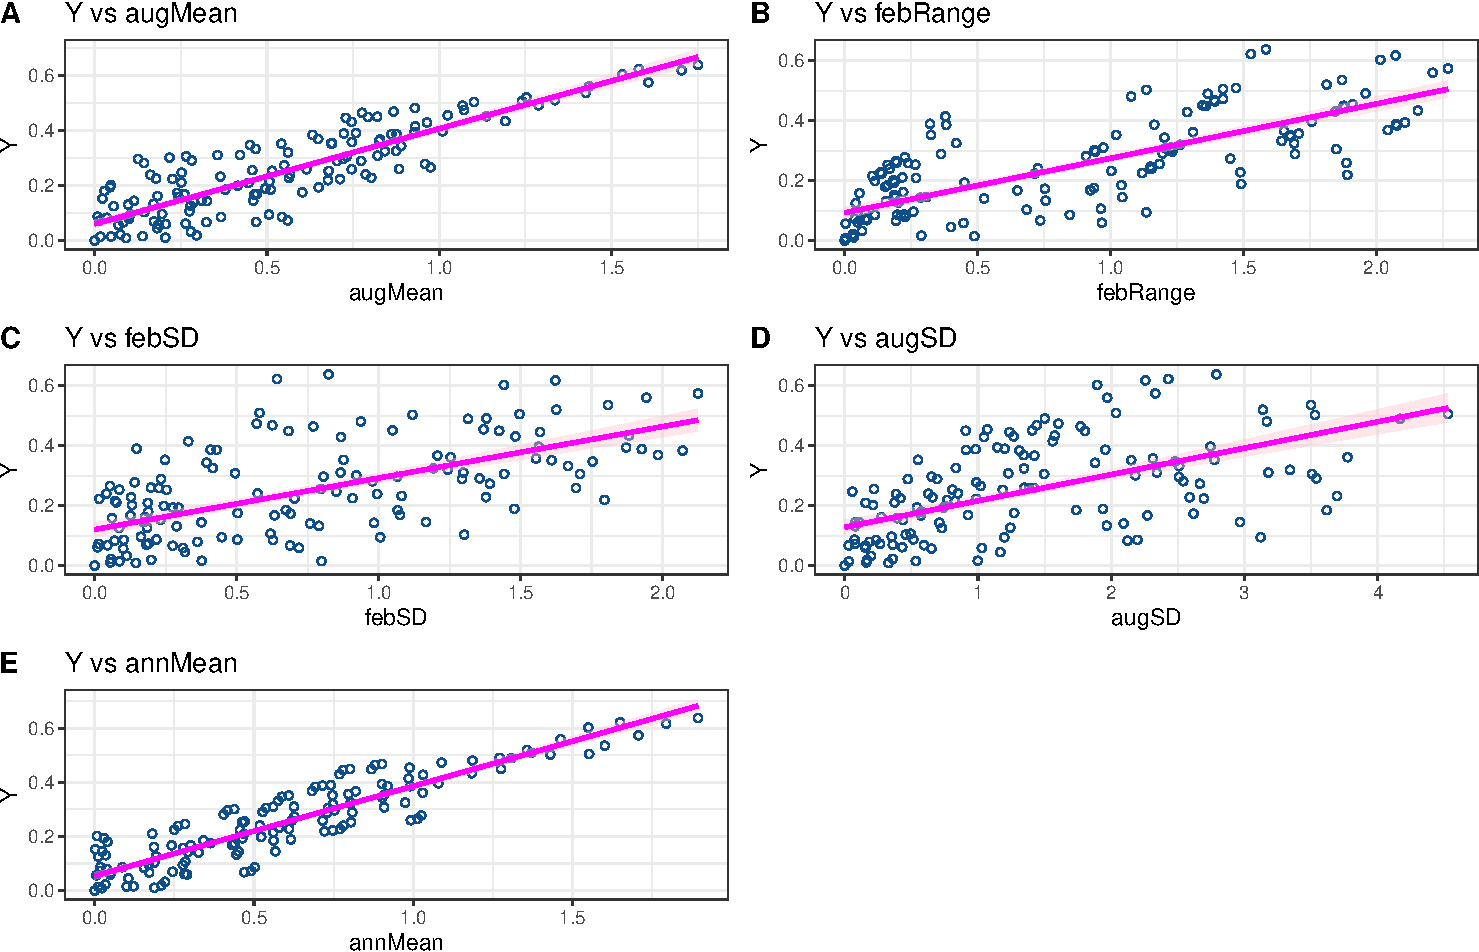
\includegraphics[keepaspectratio]{index_files/mediabag/multiple_linear_regression_files/figure-pdf/fig-slr1-1.pdf}}

}

\caption{\label{fig-slr1}Individual simple linear regressions fitted to
the variables \texttt{augMean}, \texttt{febRange}, \texttt{febSD},
\texttt{augSD}, and \texttt{annMean} as predictors of the seaweed
species composition as measured by the Sørensen dissimilarity,
\texttt{Y}.}

\end{figure}%

Figure~\ref{fig-slr1} is a series of scatter plots showing the
relationship between the response variable \(\beta_\text{sør}\) and each
of the predictor variables. The blue line represents the linear
regression fitted to the data. We see that the relationship between the
response variable and each of the predictors is positive and linear.
Each of the models are significant, as indicated by the \(p\)-values in
the model summaries. These simple models do not tell us how some
predictors might act together to influence the response variable.

To consider combined effects and interactions between predictor
variables, we must explore multiple linear regression models that
include all the predictors. Multiple regression will give us a more
integrated understanding of how various environmental variables jointly
influence species composition along the coast. In doing so, we can
control for confounding variables, improve model fit, deal with
multicollinearity, test for interaction effects, and enhance predictive
power.

We will fit this multiple regression model next.

\subsection{State the Hypotheses for a Multiple Linear
Regression}\label{state-the-hypotheses-for-a-multiple-linear-regression}

As with all inferential statistics, we need to consider the hypotheses
when performing multiple linear regression.

The null hypothesis (\(H_0\)) states that there is no significant
relationship between the Sørensen diversity index and any of the the
climatological variables entered into the model, implying that the
coefficients for all predictors are equal to zero. The alternative
hypothesis (\(H_A\)), on the other hand, states that there is a
significant relationship between the Sørensen diversity index and the
climatological variables, positing that at least one of the coefficients
is not equal to zero.

The hypotheses can be divided into two kinds: those dealing with the
main effects and the one assessing the overall model stated in
Equation~\ref{eq-full}.

\textbf{Main effects hypotheses}

The main effects hypotheses test, for each predictor, \(X_i\), if the
predictor has a significant effect on the response variable \(Y\).

\(H_0\): There is no linear relationship between the environmental
variables (\texttt{augMean}, \texttt{febRange}, \texttt{febSD},
\texttt{augSD}, and \texttt{annMean}) and the community composition as
measured by \(\beta_\text{sør}\) (in \texttt{Y}). Formally, for each
predictor variable \(X_i\):

\begin{itemize}
\tightlist
\item
  \(H_0: \beta_i = 0 \text{ for } i = 1, 2, 3, 4, 5\)
\end{itemize}

Where \(\beta_i\) are the coefficients of the predictors in the multiple
linear regression model.

\(H_A\): There is a linear relationship between the environmental
variables (\texttt{augMean}, \texttt{febRange}, \texttt{febSD},
\texttt{augSD}, and \texttt{annMean}) and the species composition as
measured by \(\beta_\text{sør}\):

\begin{itemize}
\tightlist
\item
  \(H_A: \beta_i \neq 0 \text{ for } i = 1, 2, 3, 4, 5\)
\end{itemize}

\textbf{Overall hypothesis}

In addition to testing the individual predictors, \(X_i\), we can also
test a hypothesis about the overall significance of the model
(\emph{F}-test), which examines whether the model as a whole explains a
significant amount of variance in the response variable \(Y\). A
significant \emph{F}-test would suggest that \emph{at least one}
predictor (excluding the intercept) in the model is likely to be
significantly related to the response, but it requires further
investigation of individual predictors and potential multicollinearity
to fully understand the relationships. For the overall model hypothesis:

Null Hypothesis (\(H_0\)):

\begin{itemize}
\tightlist
\item
  \(H_0: \beta_1 = \beta_2 = \beta_3 = \beta_4 = \beta_5 = 0\)
\end{itemize}

Alternative Hypothesis (\(H_A\)):

\begin{itemize}
\tightlist
\item
  \(H_A: \exists \, \beta_i \neq 0 \text{ for at least one } i\)
\end{itemize}

\subsection{Fit the Model}\label{fit-the-model}

We fit two models:

\begin{itemize}
\tightlist
\item
  a full model that includes an intercept term and the five
  environmental variables, and
\item
  a null model that includes only an intercept term.
\end{itemize}

The reason the null model is included is to compare the full model with
a model that has no predictors. This comparison will help us determine
which of the predictors are useful in explaining the response
variable---we will see this in action in the forward model selection
process later on (Section~\ref{sec-forward-selection}).

\begin{Shaded}
\begin{Highlighting}[]
\CommentTok{\# Select only the variables that will be used in model building}
\NormalTok{sw\_sub1 }\OtherTok{\textless{}{-}}\NormalTok{ sw\_ectz[, }\FunctionTok{c}\NormalTok{(}\StringTok{"Y"}\NormalTok{, }\StringTok{"augMean"}\NormalTok{, }\StringTok{"febRange"}\NormalTok{,}
                      \StringTok{"febSD"}\NormalTok{, }\StringTok{"augSD"}\NormalTok{, }\StringTok{"annMean"}\NormalTok{)]}

\CommentTok{\# Fit the full and null models}
\NormalTok{full\_mod1 }\OtherTok{\textless{}{-}} \FunctionTok{lm}\NormalTok{(Y }\SpecialCharTok{\textasciitilde{}}\NormalTok{ augMean }\SpecialCharTok{+}\NormalTok{ febRange }\SpecialCharTok{+}\NormalTok{ febSD }\SpecialCharTok{+}
\NormalTok{                 augSD }\SpecialCharTok{+}\NormalTok{ annMean, }\AttributeTok{data =}\NormalTok{ sw\_sub1)}
\NormalTok{null\_mod1 }\OtherTok{\textless{}{-}} \FunctionTok{lm}\NormalTok{(Y }\SpecialCharTok{\textasciitilde{}} \DecValTok{1}\NormalTok{, }\AttributeTok{data =}\NormalTok{ sw\_sub1)}

\CommentTok{\# Add fitted values from the full model to the dataframe}
\NormalTok{sw\_ectz}\SpecialCharTok{$}\NormalTok{.fitted }\OtherTok{\textless{}{-}} \FunctionTok{fitted}\NormalTok{(full\_mod1)}
\end{Highlighting}
\end{Shaded}

\subsection{Dealing With Multicollinearity}\label{sec-multicollinearity}

Some of the predictor variables may be correlated with each other and
this can lead to multicollinearity. When predictor variables are highly
correlated, the model may not be able to distinguish the individual
effects of each predictor. Consequently, the model becomes less precise
and harder to interpret due to the coefficients' inflated standard
errors ({[}4{]}). One can create a plot of pairwise correlations to
visually inspect the correlation structure of the predictors. I'll not
do this here, but you can try it on your own.

A formal way to detect multicollinearity is to calculate the variance
inflation factor (VIF) for each predictor variable. The VIF measures how
much the variance of the estimated regression coefficients is increased
due to multicollinearity. A VIF value greater than 5 or 10 indicates a
problematic amount of multicollinearity.

\begin{Shaded}
\begin{Highlighting}[]
\NormalTok{initial\_formula }\OtherTok{\textless{}{-}} \FunctionTok{as.formula}\NormalTok{(}\StringTok{"Y \textasciitilde{} ."}\NormalTok{)}

\NormalTok{threshold }\OtherTok{\textless{}{-}} \DecValTok{10} \CommentTok{\# Define a threshold for VIF values}

\CommentTok{\# Extract the names of the predictor variables}
\NormalTok{predictors }\OtherTok{\textless{}{-}} \FunctionTok{names}\NormalTok{(}\FunctionTok{vif}\NormalTok{(full\_mod1))}

\CommentTok{\# Iteratively remove collinear variables}
\ControlFlowTok{while}\NormalTok{ (}\ConstantTok{TRUE}\NormalTok{) \{}
  \CommentTok{\# Calculate VIF values}
\NormalTok{  vif\_values }\OtherTok{\textless{}{-}} \FunctionTok{vif}\NormalTok{(full\_mod1)}
  \FunctionTok{print}\NormalTok{(vif\_values) }\CommentTok{\# Print VIF values for debugging}
\NormalTok{  max\_vif }\OtherTok{\textless{}{-}} \FunctionTok{max}\NormalTok{(vif\_values)}
  
  \CommentTok{\# Check if the maximum VIF is above the threshold}
  \ControlFlowTok{if}\NormalTok{ (max\_vif }\SpecialCharTok{\textgreater{}}\NormalTok{ threshold) \{}
    \CommentTok{\# Find the variable with the highest VIF}
\NormalTok{    high\_vif\_var }\OtherTok{\textless{}{-}} \FunctionTok{names}\NormalTok{(}\FunctionTok{which.max}\NormalTok{(vif\_values))}
    \FunctionTok{cat}\NormalTok{(}\StringTok{"Removing variable:"}\NormalTok{,}
\NormalTok{        high\_vif\_var,}
        \StringTok{"with VIF:"}\NormalTok{,}
\NormalTok{        max\_vif,}
        \StringTok{"}\SpecialCharTok{\textbackslash{}n}\StringTok{"}\NormalTok{)}
    
    \CommentTok{\# Update the formula to exclude the high VIF variable}
\NormalTok{    updated\_formula }\OtherTok{\textless{}{-}} \FunctionTok{as.formula}\NormalTok{(}\FunctionTok{paste}\NormalTok{(}\StringTok{"Y \textasciitilde{} . {-}"}\NormalTok{, high\_vif\_var))}
    
    \CommentTok{\# Refit the model without the high VIF variable}
\NormalTok{    full\_mod1 }\OtherTok{\textless{}{-}} \FunctionTok{lm}\NormalTok{(updated\_formula, }\AttributeTok{data =}\NormalTok{ sw\_sub1)}
    
    \CommentTok{\# Update the environment data frame to reflect the removal}
\NormalTok{    sw\_sub1 }\OtherTok{\textless{}{-}}\NormalTok{ sw\_sub1[, }\SpecialCharTok{!}\NormalTok{(}\FunctionTok{names}\NormalTok{(sw\_sub1) }\SpecialCharTok{\%in\%}\NormalTok{ high\_vif\_var)]}
\NormalTok{  \} }\ControlFlowTok{else}\NormalTok{ \{}
    \ControlFlowTok{break}
\NormalTok{  \}}
\NormalTok{\}}
\SpecialCharTok{\textgreater{}}\NormalTok{   augMean  febRange     febSD     augSD   annMean }
\SpecialCharTok{\textgreater{}} \FloatTok{27.947767} \FloatTok{10.806635}  \FloatTok{8.765732}  \FloatTok{2.497739} \FloatTok{31.061900} 
\SpecialCharTok{\textgreater{}}\NormalTok{ Removing variable}\SpecialCharTok{:}\NormalTok{ annMean with VIF}\SpecialCharTok{:} \FloatTok{31.0619} 
\SpecialCharTok{\textgreater{}}\NormalTok{   augMean  febRange     febSD     augSD }
\SpecialCharTok{\textgreater{}}  \FloatTok{2.290171} \FloatTok{10.648752}  \FloatTok{8.637679}  \FloatTok{1.616390} 
\SpecialCharTok{\textgreater{}}\NormalTok{ Removing variable}\SpecialCharTok{:}\NormalTok{ febRange with VIF}\SpecialCharTok{:} \FloatTok{10.64875} 
\SpecialCharTok{\textgreater{}}\NormalTok{  augMean    febSD    augSD }
\SpecialCharTok{\textgreater{}} \FloatTok{1.423601} \FloatTok{1.674397} \FloatTok{1.585055}
\end{Highlighting}
\end{Shaded}

Regularisation techniques such as ridge regression, lasso regression, or
elastic net can also be used to deal with multicollinearity. These
advanced techniques add a penalty term to the regression model that
shrinks the coefficients towards zero, which can help to reduce the
impact of multicollinearity. However, these techniques are not covered
in this guide. Please refer to Chapter~\ref{sec-regularisation} for more
information on regularisation techniques.

\subsection{Perform Forward Selection}\label{sec-forward-selection}

It might be that not all of the variables included in the full model are
necessary to explain the response variable. We can use a stepwise
regression to select the best combination (subset) of predictors that
best explains the response variable. To do this, we will use the
\texttt{stepAIC} function that lives in the \texttt{MASS} package.

\texttt{stepAIC()} works by starting with the null model and then adding
predictors one by one, selecting the one that improves the model the
most as seen in the reduction of the AIC values along the way. This
process continues until no more predictors can be added to improve the
model (i.e.~to further reduce the AIC). Progress is tracked as the
function runs.

\begin{Shaded}
\begin{Highlighting}[]
\CommentTok{\# Perform forward selection}
\NormalTok{mod1 }\OtherTok{\textless{}{-}} \FunctionTok{stepAIC}\NormalTok{(null\_mod1,}
                \AttributeTok{scope =} \FunctionTok{list}\NormalTok{(}\AttributeTok{lower =}\NormalTok{ null\_mod1, }\AttributeTok{upper =}\NormalTok{ full\_mod1),}
                \AttributeTok{direction =} \StringTok{"forward"}\NormalTok{)}
\SpecialCharTok{\textgreater{}}\NormalTok{ Start}\SpecialCharTok{:}\NormalTok{  AIC}\OtherTok{=}\SpecialCharTok{{-}}\FloatTok{1044.97}
\SpecialCharTok{\textgreater{}}\NormalTok{ Y }\SpecialCharTok{\textasciitilde{}} \DecValTok{1}
\SpecialCharTok{\textgreater{}} 
\ErrorTok{\textgreater{}}\NormalTok{           Df Sum of Sq    RSS     AIC}
\SpecialCharTok{\textgreater{}} \SpecialCharTok{+}\NormalTok{ augMean  }\DecValTok{1}    \FloatTok{6.0084} \FloatTok{1.7108} \SpecialCharTok{{-}}\FloatTok{1478.4}
\SpecialCharTok{\textgreater{}} \SpecialCharTok{+}\NormalTok{ febSD    }\DecValTok{1}    \FloatTok{3.0759} \FloatTok{4.6433} \SpecialCharTok{{-}}\FloatTok{1189.9}
\SpecialCharTok{\textgreater{}} \SpecialCharTok{+}\NormalTok{ augSD    }\DecValTok{1}    \FloatTok{2.6394} \FloatTok{5.0797} \SpecialCharTok{{-}}\FloatTok{1163.9}
\SpecialCharTok{\textgreater{}} \ErrorTok{\textless{}}\NormalTok{none}\SpecialCharTok{\textgreater{}}                 \FloatTok{7.7192} \SpecialCharTok{{-}}\FloatTok{1045.0}
\SpecialCharTok{\textgreater{}} 
\ErrorTok{\textgreater{}}\NormalTok{ Step}\SpecialCharTok{:}\NormalTok{  AIC}\OtherTok{=}\SpecialCharTok{{-}}\FloatTok{1478.41}
\SpecialCharTok{\textgreater{}}\NormalTok{ Y }\SpecialCharTok{\textasciitilde{}}\NormalTok{ augMean}
\SpecialCharTok{\textgreater{}} 
\ErrorTok{\textgreater{}}\NormalTok{         Df Sum of Sq    RSS     AIC}
\SpecialCharTok{\textgreater{}} \SpecialCharTok{+}\NormalTok{ febSD  }\DecValTok{1}   \FloatTok{0.36036} \FloatTok{1.3504} \SpecialCharTok{{-}}\FloatTok{1544.8}
\SpecialCharTok{\textgreater{}} \SpecialCharTok{+}\NormalTok{ augSD  }\DecValTok{1}   \FloatTok{0.31243} \FloatTok{1.3984} \SpecialCharTok{{-}}\FloatTok{1534.7}
\SpecialCharTok{\textgreater{}} \ErrorTok{\textless{}}\NormalTok{none}\SpecialCharTok{\textgreater{}}               \FloatTok{1.7108} \SpecialCharTok{{-}}\FloatTok{1478.4}
\SpecialCharTok{\textgreater{}} 
\ErrorTok{\textgreater{}}\NormalTok{ Step}\SpecialCharTok{:}\NormalTok{  AIC}\OtherTok{=}\SpecialCharTok{{-}}\FloatTok{1544.77}
\SpecialCharTok{\textgreater{}}\NormalTok{ Y }\SpecialCharTok{\textasciitilde{}}\NormalTok{ augMean }\SpecialCharTok{+}\NormalTok{ febSD}
\SpecialCharTok{\textgreater{}} 
\ErrorTok{\textgreater{}}\NormalTok{         Df Sum of Sq    RSS     AIC}
\SpecialCharTok{\textgreater{}} \SpecialCharTok{+}\NormalTok{ augSD  }\DecValTok{1}   \FloatTok{0.10568} \FloatTok{1.2448} \SpecialCharTok{{-}}\FloatTok{1566.3}
\SpecialCharTok{\textgreater{}} \ErrorTok{\textless{}}\NormalTok{none}\SpecialCharTok{\textgreater{}}               \FloatTok{1.3504} \SpecialCharTok{{-}}\FloatTok{1544.8}
\SpecialCharTok{\textgreater{}} 
\ErrorTok{\textgreater{}}\NormalTok{ Step}\SpecialCharTok{:}\NormalTok{  AIC}\OtherTok{=}\SpecialCharTok{{-}}\FloatTok{1566.32}
\SpecialCharTok{\textgreater{}}\NormalTok{ Y }\SpecialCharTok{\textasciitilde{}}\NormalTok{ augMean }\SpecialCharTok{+}\NormalTok{ febSD }\SpecialCharTok{+}\NormalTok{ augSD}
\end{Highlighting}
\end{Shaded}

The model selection process shows that as we add more variables to the
model, the AIC value decreases. We can infer from this that the multiple
regression model provides a better fit that simple linear models that
use the variables in isolation.

We also see that \texttt{stepAIC()} has not removed any variables from
the full model. Probably one reason for failing to remove any variables
is that the VIF process has already accomplished this by virtue of
dealing with multicollinearity. This means that all the variables
retained in \texttt{mod1} are important in explaining the response
variable.

\subsection{Added-Variable Plots (Partial Regression
Plots)}\label{sec-added-variable-plots}

Before looking at the output in more detail, I'll introduce partial
regression plots as a means to examine the relationship between the
response variable and each predictor variable. Although they can be
calculated by hand, the \textbf{car} package provides a convenient
function, \texttt{avPlots()}, to create these plots.

Added variable plots are also sometimes called `partial regression
plots' or `individual coefficient plots.' They are used to display the
relationship between a response variable and an individual predictor
variable while accounting for the effect of other predictor variables in
a multiple regression model (the marginal effect).

\begin{Shaded}
\begin{Highlighting}[]
\CommentTok{\# Create partial regression plots}
\FunctionTok{avPlots}\NormalTok{(mod1, }\AttributeTok{col =} \StringTok{"dodgerblue4"}\NormalTok{, }\AttributeTok{col.lines =} \StringTok{"magenta"}\NormalTok{)}
\end{Highlighting}
\end{Shaded}

\begin{figure}[tbp]

\centering{

\pandocbounded{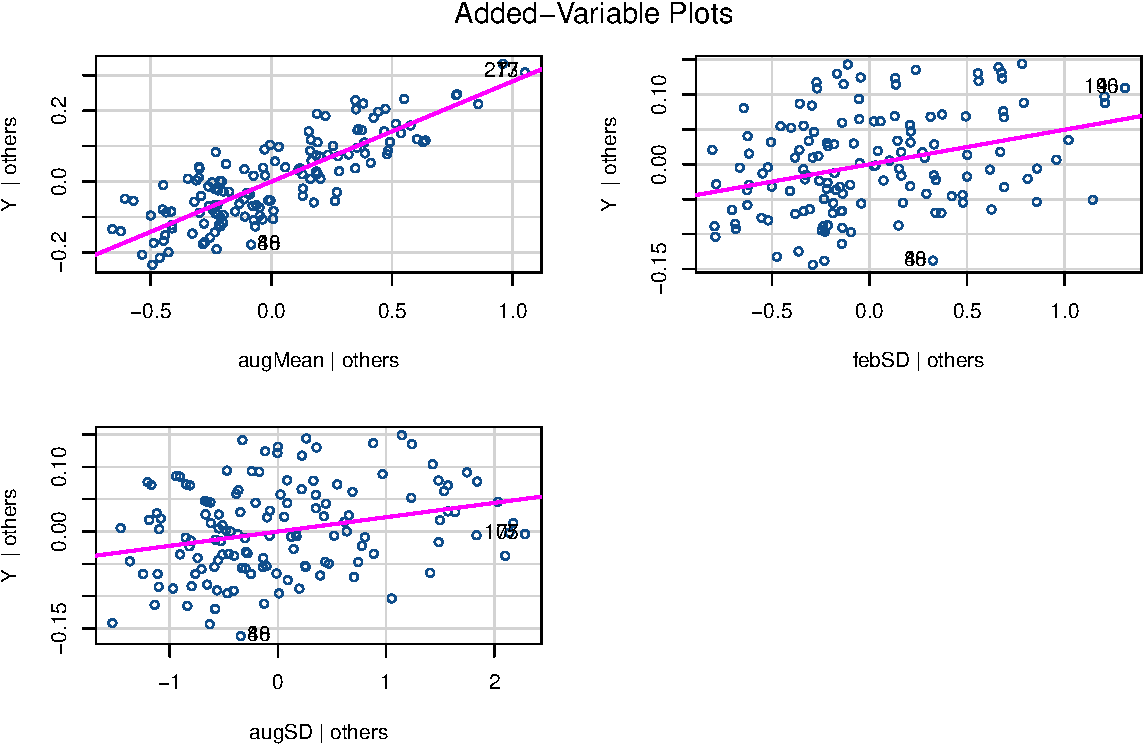
\includegraphics[keepaspectratio]{index_files/mediabag/multiple_linear_regression_files/figure-pdf/fig-mod1-partial-1.pdf}}

}

\caption{\label{fig-mod1-partial}Partial regression plots for
\texttt{mod1} with the selected variables \texttt{augMean},
\texttt{febSD}, and \texttt{augSD}.}

\end{figure}%

What insights can we draw from the added-variable plots? Although there
are better ways to assess the model fit, we can already make some
observations about the linearity of the model or the presence of
outliers. The slope of the line in an added variable plot corresponds to
the regression coefficient for that predictor in the full multiple
regression model. Seen in this way, it visually indicates the magnitude
and direction of each predictor's effect. In
Figure~\ref{fig-mod1-partial}, the added-variable plot for
\texttt{augMean} shows a tighter clustering of points around the
regression line and a strong linear relationship (steep slope) with the
response variable; the plots for \texttt{febSD} and \texttt{augSD}, on
the other hand, show a weaker response and more scatter about the
regression line. Importantly, this suggests that \texttt{augMean} has a
stronger and more unique contribution to the multiple-variable model
than the other two variables.

There are also insights to be made about possible multicollinearity
using added-variable plots. These plots are not a definitive test for
multicollinearity, but they can provide some clues. Notably, if a
predictor shows a strong relationship with the response variable in a
simple correlation but appears to have little relationship in the
added-variable plot, it might indicate collinearity with other
predictors. This discrepancy suggests that the predictor's effect on the
response is being masked by the presence of other correlated predictors.

\subsection{Model Diagnostics}\label{sec-diagnostics}

We are back in the territory of parametric statistics, so we need to
check the assumptions of the multiple linear regression model (similar
to those of simple linear regression). We can do this by making the
various diagnostic plots. all of them consider various aspects of the
residuals, which are simply the differences between the observed and
predicted values.

\textbf{Diagnostic plots of final model}

You have been introduced to diagnostic plots in the context of simple
linear regression (Section~\ref{sec-simple-linear-regression}). They are
also useful in multiple linear regression. Although \texttt{plot.lm()}
can easily do this, here I use \texttt{autoplot()} from the
\textbf{ggfortify} package. When applied to the final model,
\texttt{mod1}, the plot will in its default setting show four diagnostic
plots: residuals vs.~fitted values, normal Q-Q plot, scale-location
plot, and residuals vs.~leverage plot. Note, this is for the full model
inclusive of the combined contributions of all the predictors, so we
will not see separate plots for each predictor as we have seen in the
added-variable plots or component plus residual plots.

\begin{Shaded}
\begin{Highlighting}[]
\CommentTok{\# Generate diagnostic plots }
\FunctionTok{autoplot}\NormalTok{(mod1, }\AttributeTok{shape =} \DecValTok{21}\NormalTok{, }\AttributeTok{colour =} \StringTok{"dodgerblue4"}\NormalTok{,}
         \AttributeTok{smooth.colour =} \StringTok{"magenta"}\NormalTok{) }\SpecialCharTok{+}
  \FunctionTok{theme\_bw}\NormalTok{()}
\end{Highlighting}
\end{Shaded}

\begin{figure}[tbp]

\centering{

\pandocbounded{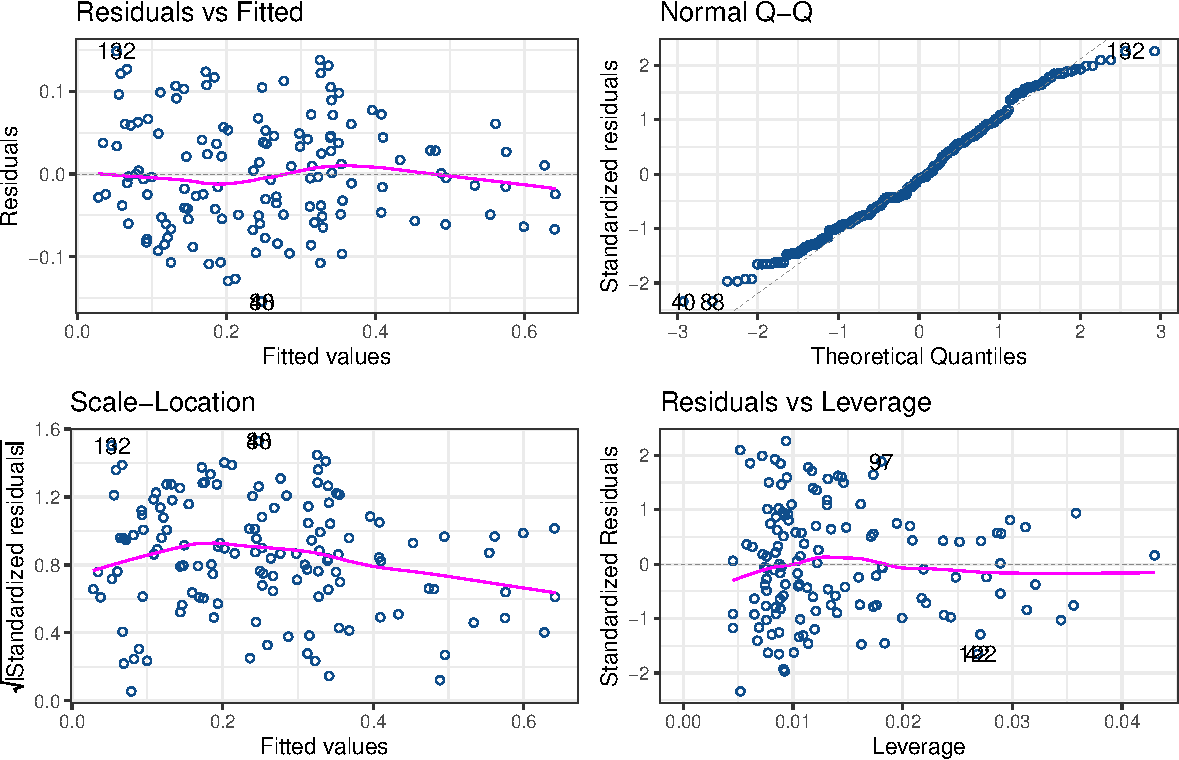
\includegraphics[keepaspectratio]{index_files/mediabag/multiple_linear_regression_files/figure-pdf/fig-mlr3-1.pdf}}

}

\caption{\label{fig-mlr3}Diagnostic plots to assess the fit of the final
multiple linear regression model, \texttt{mod1}.}

\end{figure}%

\textbf{Residuals vs.~Fitted Values:} In this plot we can assess
linearity and homoscedasticity of the residuals. If the seaweed gods
were with us, we'd expect the points to be randomly scattered about a
horizontal line situation at zero. This would indicate that the
relationship between the predictors selected by the forward selection
process (\texttt{augMean}, \texttt{febSD}, and \texttt{augSD}) and the
response variable (\texttt{Y}) is linear, and the variance of the
residuals is constant across the range of fitted values. In this plot,
there's a very slight curvature which might suggest a potential issue
with the linearity assumption---it is minute and I'd suggest not
worrying about it. The variance of the residuals seems to decrease
slightly at higher fitted values, indicating a mild case of
heteroscedasticity.

\textbf{Q-Q Plot (Quantile-Quantile Plot):} This plot is used to check
the normality of the residuals. The points should fall approximately
along a straight diagonal line if the residuals are normally
distributed. Here we see that the points generally follow the line
although some deviations may be seen at the tails. These deviations are
not that extreme and again I don't think this is not a big concern.

\textbf{Scale-Location Plot:} This plot should reveal potential issues
with homoscedasticity. The square root of the standardised residuals is
used here to make it easier to spot patterns, so we would like the
points to be randomly scattered around the horizontal red line. Here,
the line slopes slightly downward and this indicates that the variance
of the residuals might decrease as the fitted values increase. We can
also see evidence of this in a plot of the observed values vs.~the
predictors in Figure~\ref{fig-mlr3}.

\textbf{Residuals vs.~Leverage:} This diagnostic highlights influential
points (outliers). Points with high leverage (far from the mean of the
predictors) can be expected to exert a strong influence on the
regression line, tilting it in some direction. Cook's distance
(indicated by the yellow line) helps identify such outliers. In our
seaweed data a few points could have a high leverage, but since they
don't seem to cross the Cook's distance thresholds, I doubt they are
overly worrisome.

Considering that no glaring red flags were raised by the diagnostic
plots, I doubt that they are severe enough to invalidate the model.
However, if you cannot stand these small issues, you could i) consider
transforming the predictor or response variables to address your
concerns about heteroscedasticity, ii) investigate the outliers (high
leverage points) to confirm if they are valid data points or errors, or
iii) try robust regression methods that are less sensitive to outliers
and heteroscedasticity.

\textbf{Component plus residual plots}

Component plus residual plots offer another way to assess the fit of the
model in multiple regression models. Unlike simple linear regression
where we only had one predictor variable, here we have several. So, we
need to assure ourselves that there is a linear relationship between
each predictor variable and the response variable (we could already see
this in the added-variable plots in
Section~\ref{sec-added-variable-plots}). We can make component plus
residual plots using the \texttt{crPlots()} function in the \textbf{car}
package. It displays the relationship between the response variable and
each predictor variable. If the relationship is linear, the points
should be randomly scattered about a best fit line and the spline (in
pink in Figure~\ref{fig-mod1-crplots}) should plot nearly on top of the
linear regression line.

\begin{Shaded}
\begin{Highlighting}[]
\CommentTok{\# Generate component plus residual plots}
\FunctionTok{crPlots}\NormalTok{(mod1, }\AttributeTok{col =} \StringTok{"dodgerblue4"}\NormalTok{, }\AttributeTok{col.lines =} \StringTok{"magenta"}\NormalTok{)}
\end{Highlighting}
\end{Shaded}

\begin{figure}[tbp]

\centering{

\pandocbounded{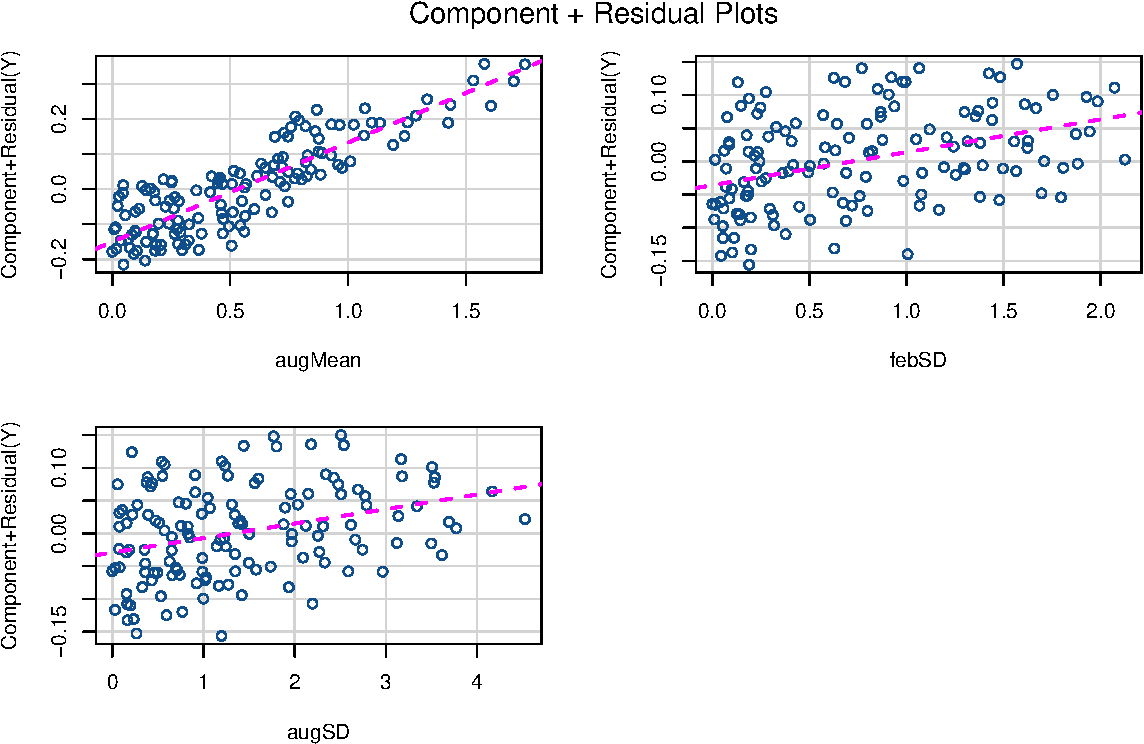
\includegraphics[keepaspectratio]{index_files/mediabag/multiple_linear_regression_files/figure-pdf/fig-mod1-crplots-1.pdf}}

}

\caption{\label{fig-mod1-crplots}Component plus residual diagnostic
plots to assess the fit of the final multiple linear regression model,
\texttt{mod1}.}

\end{figure}%

\subsection{Understanding the Model Fit}\label{sec-mod1-summary}

The above model selection process has led us to the \texttt{mod1} model,
which can be stated formally as:
\begin{equation}\phantomsection\label{eq-mod1}{Y = \alpha + \beta_1 X_1 + \beta_2 X_2 + \beta_3 X_3 + \epsilon}\end{equation}
Where:

\begin{itemize}
\tightlist
\item
  \(Y\): The response variable, the mean Sørensen dissimilarity.
\item
  \(X_1\), \(X_2\), and \(X_3\): The predictors corresponding to
  \texttt{augMean}, \texttt{febSD}, and \texttt{augSD}, respectively.
\item
  \(\epsilon\): The error term.
\end{itemize}

We have convinced ourselves that the model is a good fit for the data,
and we can proceed to examine the model's output. The fitted model can
be explored in two ways: by applying the \texttt{summary()} function or
by using the \texttt{anova()} function. The \texttt{summary()} function
provides a detailed output of the model, while the \texttt{anova()}
function provides a table of deviance values that can be used to compare
models.

\textbf{The model summary}

\begin{Shaded}
\begin{Highlighting}[]
\CommentTok{\# Summary of the selected model}
\FunctionTok{summary}\NormalTok{(mod1)}
\SpecialCharTok{\textgreater{}} 
\ErrorTok{\textgreater{}}\NormalTok{ Call}\SpecialCharTok{:}
\ErrorTok{\textgreater{}} \FunctionTok{lm}\NormalTok{(}\AttributeTok{formula =}\NormalTok{ Y }\SpecialCharTok{\textasciitilde{}}\NormalTok{ augMean }\SpecialCharTok{+}\NormalTok{ febSD }\SpecialCharTok{+}\NormalTok{ augSD, }\AttributeTok{data =}\NormalTok{ sw\_sub1)}
\SpecialCharTok{\textgreater{}} 
\ErrorTok{\textgreater{}}\NormalTok{ Residuals}\SpecialCharTok{:}
\ErrorTok{\textgreater{}}\NormalTok{       Min        }\DecValTok{1}\NormalTok{Q    Median        }\DecValTok{3}\NormalTok{Q       Max }
\SpecialCharTok{\textgreater{}} \SpecialCharTok{{-}}\FloatTok{0.153994} \SpecialCharTok{{-}}\FloatTok{0.049229} \SpecialCharTok{{-}}\FloatTok{0.006086}  \FloatTok{0.045947}  \FloatTok{0.148579} 
\SpecialCharTok{\textgreater{}} 
\ErrorTok{\textgreater{}}\NormalTok{ Coefficients}\SpecialCharTok{:}
\ErrorTok{\textgreater{}}\NormalTok{             Estimate Std. Error t value }\FunctionTok{Pr}\NormalTok{(}\SpecialCharTok{\textgreater{}}\ErrorTok{|}\NormalTok{t}\SpecialCharTok{|}\NormalTok{)    }
\SpecialCharTok{\textgreater{}}\NormalTok{ (Intercept) }\FloatTok{0.028365}   \FloatTok{0.007020}   \FloatTok{4.040} \FloatTok{6.87e{-}05} \SpecialCharTok{**}\ErrorTok{*}
\ErrorTok{\textgreater{}}\NormalTok{ augMean     }\FloatTok{0.283335}   \FloatTok{0.011131}  \FloatTok{25.455}  \SpecialCharTok{\textless{}} \FloatTok{2e{-}16} \SpecialCharTok{**}\ErrorTok{*}
\ErrorTok{\textgreater{}}\NormalTok{ febSD       }\FloatTok{0.049639}   \FloatTok{0.008370}   \FloatTok{5.930} \FloatTok{8.73e{-}09} \SpecialCharTok{**}\ErrorTok{*}
\ErrorTok{\textgreater{}}\NormalTok{ augSD       }\FloatTok{0.022150}   \FloatTok{0.004503}   \FloatTok{4.919} \FloatTok{1.47e{-}06} \SpecialCharTok{**}\ErrorTok{*}
\ErrorTok{\textgreater{}} \SpecialCharTok{{-}{-}{-}}
\ErrorTok{\textgreater{}}\NormalTok{ Signif. codes}\SpecialCharTok{:}  \DecValTok{0} \StringTok{\textquotesingle{}***\textquotesingle{}} \FloatTok{0.001} \StringTok{\textquotesingle{}**\textquotesingle{}} \FloatTok{0.01} \StringTok{\textquotesingle{}*\textquotesingle{}} \FloatTok{0.05} \StringTok{\textquotesingle{}.\textquotesingle{}} \FloatTok{0.1} \StringTok{\textquotesingle{} \textquotesingle{}} \DecValTok{1}
\SpecialCharTok{\textgreater{}} 
\ErrorTok{\textgreater{}}\NormalTok{ Residual standard error}\SpecialCharTok{:} \FloatTok{0.06609}\NormalTok{ on }\DecValTok{285}\NormalTok{ degrees of freedom}
\SpecialCharTok{\textgreater{}}\NormalTok{ Multiple R}\SpecialCharTok{{-}}\NormalTok{squared}\SpecialCharTok{:}  \FloatTok{0.8387}\NormalTok{,  Adjusted R}\SpecialCharTok{{-}}\NormalTok{squared}\SpecialCharTok{:}  \FloatTok{0.837} 
\SpecialCharTok{\textgreater{}}\NormalTok{ F}\SpecialCharTok{{-}}\NormalTok{statistic}\SpecialCharTok{:} \FloatTok{494.1}\NormalTok{ on }\DecValTok{3}\NormalTok{ and }\DecValTok{285}\NormalTok{ DF,  p}\SpecialCharTok{{-}}\NormalTok{value}\SpecialCharTok{:} \ErrorTok{\textless{}} \FloatTok{2.2e{-}16}
\end{Highlighting}
\end{Shaded}

The first part of the \texttt{summary()} function's output is the
\texttt{Coefficients} section. This is where the main effects hypotheses
are tested (this model does not have interactions---if there were,
they'd appear here, too). The important components of the coefficients
part of the model summary are:

\begin{itemize}
\tightlist
\item
  \texttt{(Intercept)}: This row provides information about where the
  regression line intersects the \emph{y}-axis.
\item
  Main Effects:

  \begin{itemize}
  \tightlist
  \item
    \texttt{augMean}, \texttt{febSD}, and \texttt{augSD}: These rows
    give the model coefficients associated with the slopes of the
    regression lines fit to those predictor variables. They indicate the
    rate of change in the response variable for a one-unit change in the
    predictor variable.
  \item
    \texttt{Estimate}, \texttt{Std.\ Error}, \texttt{t\ value}, and
    \texttt{Pr(\textgreater{}\textbar{}t\textbar{})}: These columns
    contain the statistics used to interpret the hypotheses about the
    main effects. In the \texttt{Estimate} column are the coefficients
    for the \emph{y}-intercept and the main effects' slopes, and
    \texttt{Std.\ Error} indicates the variability of the estimate. The
    \texttt{t\ value} is obtained by dividing the coefficient by its
    standard error. The \emph{p}-value tests the null hypothesis that
    the coefficient is equal to zero and significance codes are provided
    as a quick visual reference (their use is sometimes frowned upon by
    statistics purists). Using this information, we can quickly see
    that, for example, \texttt{augMean} has a coefficient of
    \(0.2833 \pm 0.0111\) and the slope of the line is highly
    significant, i.e.~there is a significant effect of \texttt{Y} due to
    the temperature gradient set up by \texttt{augMean}.
  \end{itemize}
\end{itemize}

\begin{tcolorbox}[enhanced jigsaw, opacitybacktitle=0.6, toptitle=1mm, colframe=quarto-callout-note-color-frame, arc=.35mm, left=2mm, rightrule=.15mm, coltitle=black, opacityback=0, bottomrule=.15mm, bottomtitle=1mm, title=\textcolor{quarto-callout-note-color}{\faInfo}\hspace{0.5em}{The intercept and slope coefficients}, toprule=.15mm, colbacktitle=quarto-callout-note-color!10!white, titlerule=0mm, leftrule=.75mm, colback=white, breakable]

The interpretation of the coefficients is a bit more complicated in
multiple linear regression compared to what we are accustomed to in
simple linear regression. Let us look at some greater detail at the
intercept and the slope coefficients:

Intercept (\(\alpha\)): ) The intercept is the expected value of the
response variable, \(Y\), when all predictor variables are zero. It is
not always meaningful, but it can be useful in some cases.

Slope Coefficients (\(\beta_1, \beta_2, \ldots, \beta_k\)): Each slope
coefficient, \(\beta_j\), represents the expected change in the response
variable, \(Y\), for a one-unit increase in the predictor variable,
\(X_j\), holding all other predictor variables constant. This partial
effect interpretation implies that \(\beta_j\) accounts for the direct
contribution of \(X_j\) to \(Y\) while removing the confounding effects
of other predictors in the model. Figure~\ref{fig-mod1-partial} provides
a visual representation of this concept and isolates the effect of each
predictor variable on the response variable.

Therefore, in the context of our model (Equation~\ref{eq-mod1}) for this
analysis, the partial interpretation is as follows:

\begin{itemize}
\tightlist
\item
  \(\beta_1\): Represents the change in \(Y\) for a one-unit increase in
  \(X_1\), holding \(X_2\) and \(X_3\) constant.
\item
  \(\beta_2\): Represents the change in \(Y\) for a one-unit increase in
  \(X_2\), holding \(X_1\) and \(X_3\) constant.
\item
  \(\beta_3\): Represents the change in \(Y\) for a one-unit increase in
  \(X_3\), holding \(X_1\) and \(X_2\) constant.
\end{itemize}

\end{tcolorbox}

There are also several overall model fit statistics---it is here where
you'll find the information you need to assess the hypothesis about the
overall significance of the model. \texttt{Residual\ standard\ error}
indicates the average distance between observed and fitted values.
\texttt{Multiple\ R-squared} and \texttt{Adjusted\ R-squared} values
tell us something about the model's goodness of fit. The latter adjusts
for the number of predictors in the model, and is the one you must use
and report in multiple linear regressions. As you also know, higher
numbers approaching 1 are better, with 1 suggesting that the model
perfectly captures all of the variability in the data. The
\texttt{F-statistic} and its associated \emph{p}-value test the overall
significance of the model and examines whether all regression
coefficients are simultaneously equal to zero. You can also use the
brief overview of the residuals, but I don't find this particularly
helpful---best examine the residuals in a histogram.

\textbf{The ANOVA tables}

\begin{Shaded}
\begin{Highlighting}[]
\FunctionTok{anova}\NormalTok{(mod1)}
\SpecialCharTok{\textgreater{}}\NormalTok{ Analysis of Variance Table}
\SpecialCharTok{\textgreater{}} 
\ErrorTok{\textgreater{}}\NormalTok{ Response}\SpecialCharTok{:}\NormalTok{ Y}
\SpecialCharTok{\textgreater{}}\NormalTok{            Df Sum Sq Mean Sq  F value    }\FunctionTok{Pr}\NormalTok{(}\SpecialCharTok{\textgreater{}}\NormalTok{F)    }
\SpecialCharTok{\textgreater{}}\NormalTok{ augMean     }\DecValTok{1} \FloatTok{6.0084}  \FloatTok{6.0084} \FloatTok{1375.660} \SpecialCharTok{\textless{}} \FloatTok{2.2e{-}16} \SpecialCharTok{**}\ErrorTok{*}
\ErrorTok{\textgreater{}}\NormalTok{ febSD       }\DecValTok{1} \FloatTok{0.3604}  \FloatTok{0.3604}   \FloatTok{82.507} \SpecialCharTok{\textless{}} \FloatTok{2.2e{-}16} \SpecialCharTok{**}\ErrorTok{*}
\ErrorTok{\textgreater{}}\NormalTok{ augSD       }\DecValTok{1} \FloatTok{0.1057}  \FloatTok{0.1057}   \FloatTok{24.196} \FloatTok{1.473e{-}06} \SpecialCharTok{**}\ErrorTok{*}
\ErrorTok{\textgreater{}}\NormalTok{ Residuals }\DecValTok{285} \FloatTok{1.2448}  \FloatTok{0.0044}                       
\SpecialCharTok{\textgreater{}} \SpecialCharTok{{-}{-}{-}}
\ErrorTok{\textgreater{}}\NormalTok{ Signif. codes}\SpecialCharTok{:}  \DecValTok{0} \StringTok{\textquotesingle{}***\textquotesingle{}} \FloatTok{0.001} \StringTok{\textquotesingle{}**\textquotesingle{}} \FloatTok{0.01} \StringTok{\textquotesingle{}*\textquotesingle{}} \FloatTok{0.05} \StringTok{\textquotesingle{}.\textquotesingle{}} \FloatTok{0.1} \StringTok{\textquotesingle{} \textquotesingle{}} \DecValTok{1}
\end{Highlighting}
\end{Shaded}

This function provides a sequential analysis of variance (Type I ANOVA)
table for the regression model (see more about Type I ANOVA, below). As
such, this function can also be used to compare nested models. Used on a
single model, it gives a more interpretable breakdown of the variability
in the response variable \texttt{Y} and assesses the contribution of
each predictor variable in explaining this variability.

The ANOVA table firstly shows the degrees of freedom (\texttt{Df}) for
each predictor variable added sequentially to the model, as well as the
residuals. For each predictor, the degrees of freedom is typically 1.
For the residuals, however, it represents the total number of
observations minus the number of estimated parameters. The Sum of
Squares (\texttt{Sum\ Sq}) indicates the variability in \texttt{Y}
attributable to each predictor, and the mean sum of squares
(\texttt{Mean\ Sq}) is the sum of squares divided by the degrees of
freedom.

The \texttt{F\ value} is calculated as the ratio of the predictor's mean
square to the residual mean square tests. It is used in testing the null
hypothesis that the predictor has no effect on \texttt{Y}. Whether or
not we accept the alternative hypothesis (reject the null) is given by
the \emph{p}-value (\texttt{Pr(\textgreater{}F)}) that goes with each
\emph{F}-statistic. You know how that works.

Because this is a sequential ANOVA, the amount of variance in \texttt{Y}
explained by each predictor (or group of predictors) is calculated by
adding the predictors to the model in sequence (as specified in the
model formula). For example, the Sum of Squares for \texttt{augMean}
(6.0084) represents the amount of variance explained by adding
\texttt{augMean} to a model that doesn't include any predictors yet. The
Sum of Squares for \texttt{febSD} 0.3604) represents the amount of
variance explained by adding \texttt{febSD} to a model that already
includes \texttt{augMean}---this improvement indicates that
\texttt{febSD} explains some of the variance in \texttt{Y} that
\texttt{augMean} doesn't.

\begin{tcolorbox}[enhanced jigsaw, opacitybacktitle=0.6, toptitle=1mm, colframe=quarto-callout-note-color-frame, arc=.35mm, left=2mm, rightrule=.15mm, coltitle=black, opacityback=0, bottomrule=.15mm, bottomtitle=1mm, title=\textcolor{quarto-callout-note-color}{\faInfo}\hspace{0.5em}{Order in which predictors are assessed in multiple linear regression}, toprule=.15mm, colbacktitle=quarto-callout-note-color!10!white, titlerule=0mm, leftrule=.75mm, colback=white, breakable]

The interpretation of sequential ANOVA (Type I) is inherently dependent
on the order in which predictors are entered. In \texttt{mod1} the order
is first \texttt{augMean}, then \texttt{febSD}, and last comes
\texttt{augSD}. This order might not be the most meaningful for
interpreting the sequential sums of squares and their significance in
the ANOVA table. How, then, does one decide on the order of predictors
in the model?

\begin{itemize}
\tightlist
\item
  If you have a strong theoretical or causal basis for thinking that
  certain predictors influence others, you can enter them in that order.
\item
  If you have a hierarchy of predictors based on their importance or
  general vs.~specific nature, you can enter them hierarchically.
\item
  You can manually fit models with different predictor orders and
  compare the ANOVA tables to see how the results change. This can be
  time-consuming but might offer insights into the sensitivity of your
  conclusions to the order of entry.
\item
  You can use automated model selection procedures, such as stepwise
  regression, to determine the best order of predictors. This is a more
  objective approach but can be criticised for being data-driven and not
  theory-driven.
\item
  Use Type II or Type III ANOVAs, which are are not order-dependent and
  can be used to assess the significance of predictors after accounting
  for all other predictors in the model. However, they have their own
  limitations and assumptions that need to be considered.
\end{itemize}

My advice would be to have sound theoretical reasons for the order of
predictors in the model.

\end{tcolorbox}

Both ways of looking at the model fit of
\texttt{mod1}---\texttt{summary()} and \texttt{anova()}---show that
forward selection retained the variables \texttt{augMean},
\texttt{febSD}, and \texttt{augSD}. These three predictors should be
used together to explain the response, \texttt{Y}.

Let's make a plot of the full model with all the initial predictors and
the selected model with the predictors chosen by the forward selection
process.

\begin{Shaded}
\begin{Highlighting}[]
\CommentTok{\# Add fitted values from the selected model to the dataframe}
\NormalTok{sw\_ectz}\SpecialCharTok{$}\NormalTok{.fitted\_selected }\OtherTok{\textless{}{-}} \FunctionTok{fitted}\NormalTok{(mod1)}

\CommentTok{\# Create the plot of observed vs fitted values for the selected model}
\FunctionTok{ggplot}\NormalTok{(sw\_ectz, }\FunctionTok{aes}\NormalTok{(}\AttributeTok{x =}\NormalTok{ .fitted\_selected, }\AttributeTok{y =}\NormalTok{ Y)) }\SpecialCharTok{+}
  \FunctionTok{geom\_point}\NormalTok{(}\AttributeTok{shape =} \DecValTok{1}\NormalTok{, }\AttributeTok{colour =} \StringTok{"black"}\NormalTok{, }\AttributeTok{alpha =} \FloatTok{1.0}\NormalTok{) }\SpecialCharTok{+}
  \FunctionTok{geom\_point}\NormalTok{(}\FunctionTok{aes}\NormalTok{(}\AttributeTok{x =}\NormalTok{ .fitted), }\AttributeTok{colour =} \StringTok{"red"}\NormalTok{,}
             \AttributeTok{shape =} \DecValTok{1}\NormalTok{, }\AttributeTok{alpha =} \FloatTok{0.4}\NormalTok{) }\SpecialCharTok{+}
  \FunctionTok{geom\_abline}\NormalTok{(}\AttributeTok{intercept =} \DecValTok{0}\NormalTok{, }\AttributeTok{slope =} \DecValTok{1}\NormalTok{,}
              \AttributeTok{color =} \StringTok{"blue"}\NormalTok{, }\AttributeTok{linetype =} \StringTok{"dashed"}\NormalTok{) }\SpecialCharTok{+}
  \FunctionTok{labs}\NormalTok{(}\AttributeTok{x =} \StringTok{"Fitted Values"}\NormalTok{,}
       \AttributeTok{y =} \StringTok{"Observed Values"}\NormalTok{) }\SpecialCharTok{+}
  \FunctionTok{theme\_bw}\NormalTok{()}
\end{Highlighting}
\end{Shaded}

\begin{figure}[tbp]

\centering{

\pandocbounded{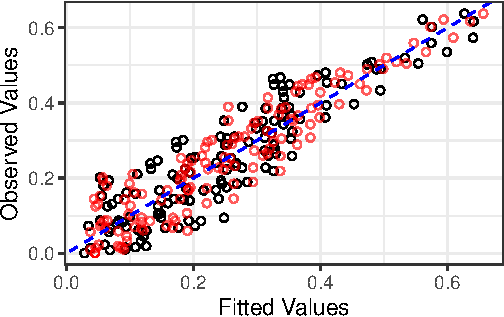
\includegraphics[keepaspectratio]{index_files/mediabag/multiple_linear_regression_files/figure-pdf/fig-mlr2-1.pdf}}

}

\caption{\label{fig-mlr2}Plot of observed vs.~predicted value obtained
from the final multiple linear regression model (\texttt{mod}) with the
selected variables \texttt{augMean}, \texttt{febSD}, and \texttt{augSD}
as predictors (black points), and the initial model with also
\texttt{annMean} and \texttt{febRange} (red points).}

\end{figure}%

\subsection{Reporting}\label{reporting-1}

A Results section should be written in a format sutable for inclusion in
your report or publication. Present the results in a clear and concise
manner, with tables and figures used to help substantiate your findings.
The results should be interpreted in the context of the research
question and the study design. The limitations of the analysis should
also be discussed, along with any potential sources of bias or
confounding. Here is an example.

\textbf{Results}

The model demonstrates a strong overall fit, as indicated by the high
\(R^2\) value of 0.839 and an adjusted \(R^2\) of 0.837, suggesting that
approximately 83.7\% of the variance in the mean Sørensen dissimilarity
is explained by the predictors \texttt{augMean}, \texttt{febSD}, and
\texttt{augSD}. All predictors in the model are statistically
significant, with \texttt{augMean} showing the strongest effect
(\(\beta_1 = 0.283\), \(p < 0.0001\)) (Figure~\ref{fig-mod1-partial}).
The predictors \texttt{febSD} and \texttt{augSD} also have significant
positive relationships with the response variable (\(\beta_2 = 0.050\),
\(p = 0.0001\); \(\beta_3 = 0.022\), \(p = 0.0001\)). A sequential ANOVA
further confirms the significance of each predictor variable in the
model, with all \emph{F}-values indicating that the inclusion of each
predictor significantly improves the model fit (\(p < 0.0001\) in all
cases). Our model therefore provides clear support for the mean
temperatures in August, the standard deviation of temperatures in
February, and the standard deviation of temperatures in August as strong
predictors of the mean Sørensen dissimilarity, with each contributing
uniquely to the explanation of variability in the response variable.

\section{Example 2: Interaction of Distance and
Bioregion}\label{sec-mlr-interaction}

Our seaweed dataset includes two additional variables that we have not
yet considered. These are the continuous variable \texttt{dist} which
represents the geographic distance between the seaweed samples taken
along the coast of South Africa, and the categorical variable
\texttt{bio} which is the bioregional classification of the seaweed
samples.

These two new variables lend themselves to a few interesting questions.
For example:

\begin{enumerate}
\def\labelenumi{\arabic{enumi}.}
\tightlist
\item
  Is the geographic distance between samples related to the Sørensens
  dissimilarity of the seaweed flora?
\item
  Does the average Sørensens dissimilarity vary among the bioregions to
  which the samples belong?
\item
  Is the effect of geographic distance on the Sørensens dissimilarity
  different for each bioregion?
\end{enumerate}

The most complex model is (3), the one that answers the question about
whether the effect of \texttt{dist} on the response variable \(Y\) is
different for each bioregion. Questions (1) and (2) are subsets of this
more inclusive question. To fully answer these quesitons, let's first
consider the full model, which includes an \emph{interaction term}
between the continuous predictor \texttt{dist} and the categorical
predictor \texttt{bio}. When we finally test our model, we will also
have to consider the simpler models that do not include the interaction
term.

`Interaction' means that the effect of one predictor on the response
variable is contingent on the value of another predictor. For example,
we might have reason to suspect that the relationship of the Sørensens
dissimilarity with the geographic distance between samples is different
between the west coast compared to, say, the east coast. This is indeed
a plausible expectation, but we will test this formally below.

The full multiple linear regression model with the interaction terms can
be formally expressed as Equation \ref{mod2}:

\begin{align}
Y &= \alpha + \beta_1 \text{dist} + \beta_2 \text{bio}_{\text{B-ATZ}} + \beta_3 \text{bio}_{\text{BMP}} \nonumber \\
  &\quad + \beta_4 \text{bio}_{\text{ECTZ}} + \beta_5 (\text{dist} \times \text{bio}_{\text{B-ATZ}}) \nonumber \\
  &\quad + \beta_6 (\text{dist} \times \text{bio}_{\text{BMP}}) + \beta_7 (\text{dist} \times \text{bio}_{\text{ECTZ}}) + \epsilon \label{mod2}
\end{align}

Where:

\begin{itemize}
\tightlist
\item
  \(Y\): The response variable, the mean Sørensen dissimilarity.
\item
  \(\alpha\): The intercept term.
\item
  \(\text{dist}\): The continuous predictor variable representing
  distance.
\item
  \(\text{bio}\): The categorical predictor variable representing
  bioregional classification with four levels: \texttt{AMP} (reference
  category), \texttt{B-ATZ}, \texttt{BMP}, and \texttt{ECTZ}.
\item
  \(\text{bio}_\text{B-ATZ}, \text{bio}_\text{BMP}, \text{bio}_\text{ECTZ}\):
  Dummy variables for the bioregional classification, where:

  \begin{itemize}
  \tightlist
  \item
    \(\text{bio}_\text{B-ATZ} = 1\) if \texttt{bio} = \texttt{B-ATZ},
    and 0 otherwise,
  \item
    \(\text{bio}_\text{BMP} = 1\) if \texttt{bio} = \texttt{BMP}, and 0
    otherwise, and
  \item
    \(\text{bio}_\text{ECTZ} = 1\) if \texttt{bio} = \texttt{ECTZ}, and
    0 otherwise.
  \end{itemize}
\item
  \(\text{dist} \times \text{bio}_\text{B-ATZ}, \text{dist} \times \text{bio}_\text{BMP}, \text{dist} \times \text{bio}_\text{ECTZ}\):
  Interaction terms between distance and the bioregional classification
  dummy variables.
\item
  \(\beta_1, \beta_2, \beta_3, \beta_4, \beta_5, \beta_6, \beta_7\): The
  coefficients to be estimated for the main effects and interactions.
\item
  \(\epsilon\): The error term.
\end{itemize}

If this seems tricky, it is because of the dummy variable coding used to
represent interactions in multiple linear regression. The \texttt{bio}
variable is a categorical variable with four levels, so we need to
create three dummy variables to represent the bioregional
classification. The \texttt{dist} variable is then interacted with each
of these dummy variables to create the interaction terms. The
\texttt{lm()} function in R takes care of this for us in a far less
complicated model statement. I'll explain the details around the
interpretation of dummy variable coding when we look at the output of
the model with the \texttt{summary()} function.

\subsection{State the Hypotheses for a Multiple Linear Regression with
Interaction
Terms}\label{state-the-hypotheses-for-a-multiple-linear-regression-with-interaction-terms}

Equation \ref{mod2} expands into the following series of hypotheses that
concern the main effects, the interactions between the main effects, and
the overall hypothesis:

\textbf{Main effects hypotheses}

In the main effects hypotheses we are concerned with the effect of each
predictor variable on the response variable. For the main effect of
distance we have the null:

\begin{itemize}
\tightlist
\item
  \(H_0: \beta_1 = 0\)
\end{itemize}

vs.~the alternative:

\begin{itemize}
\tightlist
\item
  \(H_A: \beta_1 \neq 0\)
\end{itemize}

For the main effect of bioregional classification, the nulls are:

\begin{itemize}
\tightlist
\item
  \(H_0: \beta_2 = 0 \quad (\text{bio}_{\text{B-ATZ}})\)
\item
  \(H_0: \beta_3 = 0 \quad (\text{bio}_{\text{BMP}})\)
\item
  \(H_0: \beta_4 = 0 \quad (\text{bio}_{\text{ECTZ}})\)
\end{itemize}

vs.~the alternatives:

\begin{itemize}
\tightlist
\item
  \(H_A: \beta_2 \neq 0 \quad (\text{bio}_{\text{B-ATZ}})\)
\item
  \(H_A: \beta_3 \neq 0 \quad (\text{bio}_{\text{BMP}})\)
\item
  \(H_A: \beta_4 \neq 0 \quad (\text{bio}_{\text{ECTZ}})\)
\end{itemize}

\textbf{Hypotheses about interactions}

This is where the hypothesis tests whether the effect of distance on the
response variable is different for each bioregional classification. The
null hypotheses are:

\begin{itemize}
\tightlist
\item
  \(H_0: \beta_5 = 0 \quad (\text{dist} \times \text{bio}_{\text{B-ATZ}})\)
\item
  \(H_0: \beta_6 = 0 \quad (\text{dist} \times \text{bio}_{\text{BMP}})\)
\item
  \(H_0: \beta_7 = 0 \quad (\text{dist} \times \text{bio}_{\text{ECTZ}})\)
\end{itemize}

vs.~the alternatives:

\begin{itemize}
\tightlist
\item
  \(H_A: \beta_5 \neq 0 \quad (\text{dist} \times \text{bio}_{\text{B-ATZ}})\)
\item
  \(H_A: \beta_6 \neq 0 \quad (\text{dist} \times \text{bio}_{\text{BMP}})\)
\item
  \(H_A: \beta_7 \neq 0 \quad (\text{dist} \times \text{bio}_{\text{ECTZ}})\)
\end{itemize}

\textbf{Overall hypothesis}

The overall hypothesis states that all coefficients associated with the
predictors (distance, bioregional categories, and their interactions)
are equal to zero, therefore indicating no relationship between these
predictors and the response variable, the Sørensen index. The null
hypothesis is:

\begin{itemize}
\tightlist
\item
  \(H_0: \beta_1 = \beta_2 = \beta_3 = \beta_4 = \beta_5 = \beta_6 = \beta_7 = 0\)
\end{itemize}

vs.~the alternative:

\begin{itemize}
\tightlist
\item
  \(H_A: \exists \, \beta_i \neq 0 \text{ for at least one } i\)
\end{itemize}

\begin{figure}[tbp]

\centering{

\pandocbounded{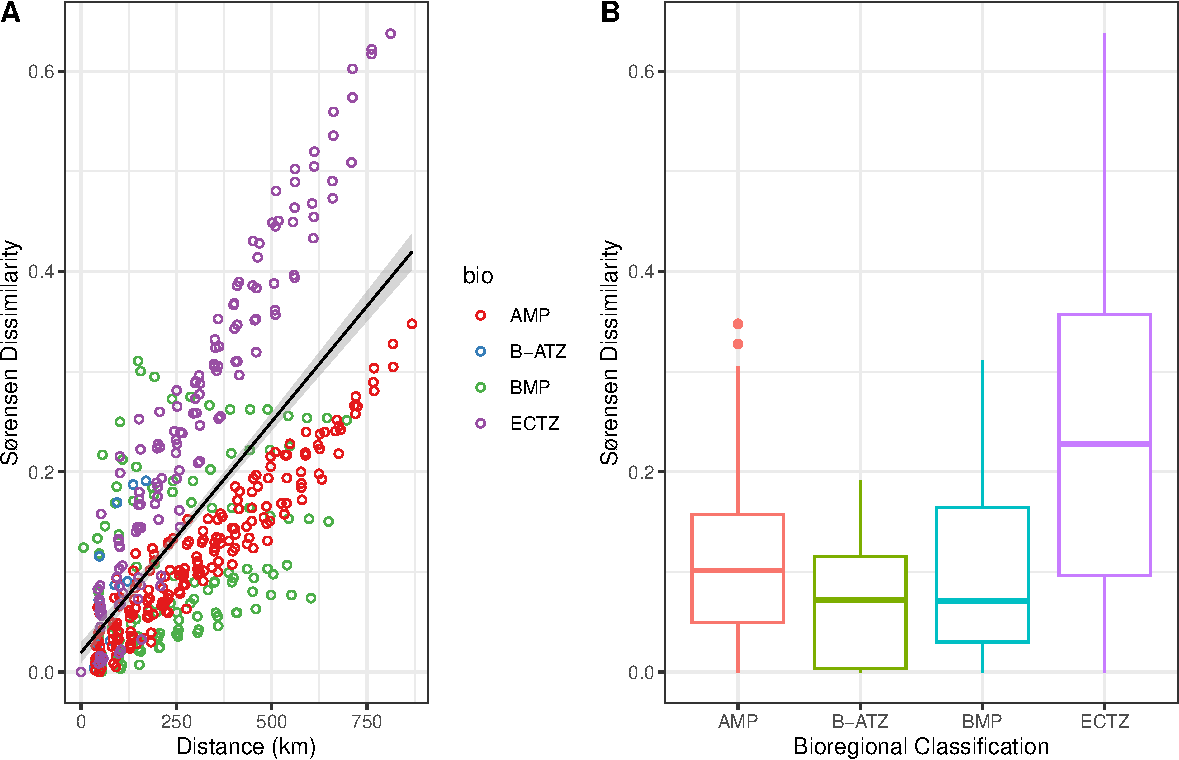
\includegraphics[keepaspectratio]{index_files/mediabag/multiple_linear_regression_files/figure-pdf/fig-mod2_main_effects-1.pdf}}

}

\caption{\label{fig-mod2_main_effects}Plot of main effects of A)
distance along the coast and B) bioregional classification on the
Sørensen dissimilarity index.}

\end{figure}%

\subsection{Visualise the Main
Effects}\label{visualise-the-main-effects}

To facilitate the interpretation of the main effects hypotheses and make
an argument for why an interaction term might be necessary, I've
visualised the main effects (Figure~\ref{fig-mod2_main_effects}). I see
this as part of my exploratory data analysis ensemble of tests. We see
that fitting a straight line to the \texttt{Y} vs.~distance relationship
seems unsatisfactory as there is too much scatter around that single
line to adequately capture all the structure in the variability of the
points. Colouring the points by bioregion reveals the hidden structure.
The model could benefit from including an additional level of
complexity: see how points in the same bioregion show less scatter
compared to points in different bioregions.

Now look at the boxplots of the Sørensen dissimilarity index for each
bioregional classification. It shows that the median values of the
Sørensen dissimilarity index are different for each bioregion. Taken
together, Figure~\ref{fig-mod2_main_effects} (A, B) provide a good
indication that adding the bioregional classification might be an
important predictor of the Sørensen dissimilarity index as a function of
distance between pairs of sites along the coast.

Next, we will move ahead and fit the model inclusive of the distance
along the coast and bioregion as per Equation \eqref{mod2}.

\subsection{Fit and Assess Nested
Models}\label{fit-and-assess-nested-models}

I have a suspicion that the full model (\texttt{mod2}; see below) with
the interaction terms will be a better fit than reduced models with only
the effect due to distance (seen independently). How can we have greater
certainty that we should indeed favour a slightly more complex model
(with two predictors) over a simpler one with only (distance only)?

One way to do this is to use a nested model comparison. We will fit a
reduced model (one slope for all bioregions) and compare this model to
the full model (slopes are allowed to vary among bioregions).

\begin{Shaded}
\begin{Highlighting}[]
\CommentTok{\# Fit the linear regression model with only distance}
\NormalTok{mod2a }\OtherTok{\textless{}{-}} \FunctionTok{lm}\NormalTok{(Y }\SpecialCharTok{\textasciitilde{}}\NormalTok{ dist, }\AttributeTok{data =}\NormalTok{ sw)}

\CommentTok{\# Fit the multiple linear regression model with interaction terms}
\NormalTok{mod2 }\OtherTok{\textless{}{-}} \FunctionTok{lm}\NormalTok{(Y }\SpecialCharTok{\textasciitilde{}}\NormalTok{ dist }\SpecialCharTok{*}\NormalTok{ bio, }\AttributeTok{data =}\NormalTok{ sw)}
\end{Highlighting}
\end{Shaded}

This is a nested model where \texttt{mod2a} is nested within
\texttt{mod2}. `Nested' means that the reduced model is a subset of the
full model. Nested models can be used to test hypotheses about the
significance of the predictors in the full model---does adding more
predictors to the model improve the fit? Comparing a nested model with a
full model can be done with a sequential ANOVA, which is what the
\texttt{anova()} function also does (in addition to its use in
Section~\ref{sec-mod1-summary}).

So, comparing \texttt{mod2a} to \texttt{mod2} with an \emph{F}-test
tests the significance of adding the \texttt{bio} and using it together
with \texttt{dist}. The interaction is built into \texttt{mod2} but we
are not yet testing the significance of the interaction terms. We will
do that later.

\begin{Shaded}
\begin{Highlighting}[]
\FunctionTok{anova}\NormalTok{(mod2a, mod2, }\AttributeTok{test =} \StringTok{"F"}\NormalTok{)}
\SpecialCharTok{\textgreater{}}\NormalTok{ Analysis of Variance Table}
\SpecialCharTok{\textgreater{}} 
\ErrorTok{\textgreater{}}\NormalTok{ Model }\DecValTok{1}\SpecialCharTok{:}\NormalTok{ Y }\SpecialCharTok{\textasciitilde{}}\NormalTok{ dist}
\SpecialCharTok{\textgreater{}}\NormalTok{ Model }\DecValTok{2}\SpecialCharTok{:}\NormalTok{ Y }\SpecialCharTok{\textasciitilde{}}\NormalTok{ dist }\SpecialCharTok{*}\NormalTok{ bio}
\SpecialCharTok{\textgreater{}}\NormalTok{   Res.Df    RSS Df Sum of Sq      F    }\FunctionTok{Pr}\NormalTok{(}\SpecialCharTok{\textgreater{}}\NormalTok{F)    }
\SpecialCharTok{\textgreater{}} \DecValTok{1}    \DecValTok{968} \FloatTok{7.7388}                                  
\SpecialCharTok{\textgreater{}} \DecValTok{2}    \DecValTok{962} \FloatTok{2.2507}  \DecValTok{6}    \FloatTok{5.4881} \FloatTok{390.95} \SpecialCharTok{\textless{}} \FloatTok{2.2e{-}16} \SpecialCharTok{**}\ErrorTok{*}
\ErrorTok{\textgreater{}} \SpecialCharTok{{-}{-}{-}}
\ErrorTok{\textgreater{}}\NormalTok{ Signif. codes}\SpecialCharTok{:}  \DecValTok{0} \StringTok{\textquotesingle{}***\textquotesingle{}} \FloatTok{0.001} \StringTok{\textquotesingle{}**\textquotesingle{}} \FloatTok{0.01} \StringTok{\textquotesingle{}*\textquotesingle{}} \FloatTok{0.05} \StringTok{\textquotesingle{}.\textquotesingle{}} \FloatTok{0.1} \StringTok{\textquotesingle{} \textquotesingle{}} \DecValTok{1}
\end{Highlighting}
\end{Shaded}

The sequential ANOVA shows that there is significant merit to consider
an interaction term in the model. This model would then allow us to have
a separate slope for the Sørensen index as function of distance for each
bioregion. The residual sum of squares (\texttt{RSS}) decreases from
7.7388 in Model 1 to 2.2507 in Model 2, which indicates that Model 2
explains a significantly larger proportion of the variance in the
response variable. The \emph{F}-test for comparing the two models yields
an \emph{F}-value of 390.95 with a highly significant \emph{p}-value
(\textless{} 0.0001). The improvement in model fit due to the inclusion
of the interaction term is therefore statistically significant.

The above analyses skirted around the questions stated in the beginning
of Section~\ref{sec-mlr-interaction}. I've provided statistical evidence
that full model is a better fit than the reduced model (the sequential
\emph{F}-test tested this), so we should use both \texttt{dist} and
\texttt{bio} in the model. I have not looked explicitly at the main
effects of the predictors. However, we can easily address questions (1)
and (2):

\begin{itemize}
\tightlist
\item
  Question 1: looking at the summary of \texttt{mod2a} tells us that the
  main effect of \texttt{dist} is a significant (\emph{p} \textless{}
  0.0001) predictor of the Sørensen dissimilarity index.
\item
  Question 2: the main effect of \texttt{bio} is also significant
  (\emph{p} \textless{} 0.0001), which is what we'd see if we fit the
  model
  \texttt{mod2b\ \textless{}-\ lm(Y\ \textasciitilde{}\ bio,\ data\ =\ sw)}.
\end{itemize}

Question 3 warrants deeper investigation. Next, we will look at the
interaction terms in the full model \texttt{mod2} to see if the effect
of \texttt{dist} on \texttt{Y} is different for each level of
\texttt{bio}.

\subsection{Interpret the Full Model}\label{interpret-the-full-model}

\textbf{The model summary}

\begin{Shaded}
\begin{Highlighting}[]
\CommentTok{\# Summary of the model}
\FunctionTok{summary}\NormalTok{(mod2)}
\SpecialCharTok{\textgreater{}} 
\ErrorTok{\textgreater{}}\NormalTok{ Call}\SpecialCharTok{:}
\ErrorTok{\textgreater{}} \FunctionTok{lm}\NormalTok{(}\AttributeTok{formula =}\NormalTok{ Y }\SpecialCharTok{\textasciitilde{}}\NormalTok{ dist }\SpecialCharTok{*}\NormalTok{ bio, }\AttributeTok{data =}\NormalTok{ sw)}
\SpecialCharTok{\textgreater{}} 
\ErrorTok{\textgreater{}}\NormalTok{ Residuals}\SpecialCharTok{:}
\ErrorTok{\textgreater{}}\NormalTok{       Min        }\DecValTok{1}\NormalTok{Q    Median        }\DecValTok{3}\NormalTok{Q       Max }
\SpecialCharTok{\textgreater{}} \SpecialCharTok{{-}}\FloatTok{0.112117} \SpecialCharTok{{-}}\FloatTok{0.030176} \SpecialCharTok{{-}}\FloatTok{0.004195}  \FloatTok{0.023698}  \FloatTok{0.233520} 
\SpecialCharTok{\textgreater{}} 
\ErrorTok{\textgreater{}}\NormalTok{ Coefficients}\SpecialCharTok{:}
\ErrorTok{\textgreater{}}\NormalTok{                 Estimate Std. Error t value }\FunctionTok{Pr}\NormalTok{(}\SpecialCharTok{\textgreater{}}\ErrorTok{|}\NormalTok{t}\SpecialCharTok{|}\NormalTok{)    }
\SpecialCharTok{\textgreater{}}\NormalTok{ (Intercept)    }\FloatTok{5.341e{-}03}  \FloatTok{4.177e{-}03}   \FloatTok{1.279}   \FloatTok{0.2013}    
\SpecialCharTok{\textgreater{}}\NormalTok{ dist           }\FloatTok{3.530e{-}04}  \FloatTok{1.140e{-}05}  \FloatTok{30.958}  \SpecialCharTok{\textless{}} \FloatTok{2e{-}16} \SpecialCharTok{**}\ErrorTok{*}
\ErrorTok{\textgreater{}}\NormalTok{ bioB}\SpecialCharTok{{-}}\NormalTok{ATZ      }\SpecialCharTok{{-}}\FloatTok{6.140e{-}03}  \FloatTok{1.659e{-}02}  \SpecialCharTok{{-}}\FloatTok{0.370}   \FloatTok{0.7114}    
\SpecialCharTok{\textgreater{}}\NormalTok{ bioBMP         }\FloatTok{3.820e{-}02}  \FloatTok{6.659e{-}03}   \FloatTok{5.737} \FloatTok{1.29e{-}08} \SpecialCharTok{**}\ErrorTok{*}
\ErrorTok{\textgreater{}}\NormalTok{ bioECTZ        }\FloatTok{1.629e{-}02}  \FloatTok{6.447e{-}03}   \FloatTok{2.527}   \FloatTok{0.0117} \SpecialCharTok{*}  
\ErrorTok{\textgreater{}}\NormalTok{ dist}\SpecialCharTok{:}\NormalTok{bioB}\SpecialCharTok{{-}}\NormalTok{ATZ  }\FloatTok{7.976e{-}04}  \FloatTok{1.875e{-}04}   \FloatTok{4.255} \FloatTok{2.30e{-}05} \SpecialCharTok{**}\ErrorTok{*}
\ErrorTok{\textgreater{}}\NormalTok{ dist}\SpecialCharTok{:}\NormalTok{bioBMP   }\SpecialCharTok{{-}}\FloatTok{1.285e{-}04}  \FloatTok{2.065e{-}05}  \SpecialCharTok{{-}}\FloatTok{6.222} \FloatTok{7.31e{-}10} \SpecialCharTok{**}\ErrorTok{*}
\ErrorTok{\textgreater{}}\NormalTok{ dist}\SpecialCharTok{:}\NormalTok{bioECTZ   }\FloatTok{4.213e{-}04}  \FloatTok{1.801e{-}05}  \FloatTok{23.392}  \SpecialCharTok{\textless{}} \FloatTok{2e{-}16} \SpecialCharTok{**}\ErrorTok{*}
\ErrorTok{\textgreater{}} \SpecialCharTok{{-}{-}{-}}
\ErrorTok{\textgreater{}}\NormalTok{ Signif. codes}\SpecialCharTok{:}  \DecValTok{0} \StringTok{\textquotesingle{}***\textquotesingle{}} \FloatTok{0.001} \StringTok{\textquotesingle{}**\textquotesingle{}} \FloatTok{0.01} \StringTok{\textquotesingle{}*\textquotesingle{}} \FloatTok{0.05} \StringTok{\textquotesingle{}.\textquotesingle{}} \FloatTok{0.1} \StringTok{\textquotesingle{} \textquotesingle{}} \DecValTok{1}
\SpecialCharTok{\textgreater{}} 
\ErrorTok{\textgreater{}}\NormalTok{ Residual standard error}\SpecialCharTok{:} \FloatTok{0.04837}\NormalTok{ on }\DecValTok{962}\NormalTok{ degrees of freedom}
\SpecialCharTok{\textgreater{}}\NormalTok{ Multiple R}\SpecialCharTok{{-}}\NormalTok{squared}\SpecialCharTok{:}  \FloatTok{0.8607}\NormalTok{,  Adjusted R}\SpecialCharTok{{-}}\NormalTok{squared}\SpecialCharTok{:}  \FloatTok{0.8597} 
\SpecialCharTok{\textgreater{}}\NormalTok{ F}\SpecialCharTok{{-}}\NormalTok{statistic}\SpecialCharTok{:} \FloatTok{849.2}\NormalTok{ on }\DecValTok{7}\NormalTok{ and }\DecValTok{962}\NormalTok{ DF,  p}\SpecialCharTok{{-}}\NormalTok{value}\SpecialCharTok{:} \ErrorTok{\textless{}} \FloatTok{2.2e{-}16}
\end{Highlighting}
\end{Shaded}

In the output returned by \texttt{summary(mod2)}, we need to pay special
attention to the use of dummy variable encoding for the categorical
predictor. The \texttt{Coefficients} section is similar to that of
\texttt{mod1} (see Section~\ref{sec-mod1-summary}), but now it includes
the categorical predictor \texttt{bio*} and the interaction terms
\texttt{dist:bio*} (\texttt{*} indicating the levels of the categorical
variable). The \texttt{bio} variable has four levels, \texttt{BMP},
\texttt{B-ATZ}, \texttt{AMP}, and \texttt{ECTZ}, and \texttt{AMP} is
selected as reference level. This decision to selected \texttt{AMP} as
reference is entirely arbitrary, and alphabetical sorting offers a
convenient approach to selecting the reference. The coefficients for the
other levels of \texttt{bio} are interpreted as the sum of the response
variable and the reference level.

The following are the key coefficients in the model summary:

\begin{itemize}
\tightlist
\item
  \texttt{(Intercept)}: This is the estimated average value of
  \texttt{Y} when \texttt{dist} is zero and \texttt{bio} is the
  reference category (\texttt{AMP}). Its \emph{p}-value (\textgreater{}
  0.05) suggests it's not significantly different from zero.
\item
  Main Effects:

  \begin{itemize}
  \tightlist
  \item
    \texttt{dist}: This represents the estimated change in \texttt{Y}
    for a one-unit increase in \texttt{dist} when the bioregion is the
    reference category, \texttt{AMP}. The highly significant
    \emph{p}-value (\textless{} 0.0001) indicates a strong effect of
    distance in the \texttt{AMP}.
  \item
    \texttt{bioB-ATZ}, \texttt{bioBMP}, \texttt{bioECTZ}: These are
    dummy variables representing different bioregions. Their
    coefficients indicate the difference in the average value of
    \texttt{Y} between each of these bioregions and the reference
    bioregion when \texttt{dist} is zero. Only \texttt{bioBMP} and
    \texttt{bioECTZ} are significantly different from the reference
    bioregion, \texttt{AMP}.
  \end{itemize}
\item
  Interaction Effects:

  \begin{itemize}
  \tightlist
  \item
    \texttt{dist:bioB-ATZ}, \texttt{dist:bioBMP}, \texttt{dist:bioECTZ}:
    These interaction terms capture how the effect of \texttt{dist} on
    \texttt{Y} varies across different bioregions. For instance,
    \texttt{dist:bioB-ATZ} indicates the additional change in the effect
    of \texttt{dist} in the \texttt{B-ATZ} bioregion compared to the
    reference bioregion, \texttt{AMP}. All interaction terms are highly
    significant, suggesting the effect of distance is different across
    bioregions.
  \end{itemize}
\end{itemize}

Given this explanation, we can now interpret the coefficients of, for
example, the \texttt{bioB-ATZ} main effect and \texttt{dist:bioB-ATZ}
interaction. Since \texttt{AMP} is the reference bioregion, its effect
is absorbed into the intercept term. Therefore, the coefficient for
\texttt{bioB-ATZ} directly reflects the difference we are interested in.
The coefficient for \texttt{bioB-ATZ} is -0.0061 \(\pm\) 0.0166 lower
than that of the reference, but the associated \emph{p}-value
(\textgreater{} 0.05) indicates that the average value of \texttt{Y} in
the \texttt{B-ATZ} bioregion is not significantly different from the
reference bioregion, \texttt{AMP}.

If we'd want to report the actual coefficient for \texttt{B-ATZ}, we'd
calculate the sum of the coefficients for \texttt{(Intercept)} and
\texttt{bioB-ATZ}. This would give us the estimated average value of
\texttt{Y} in the \texttt{B-ATZ} bioregion when \texttt{dist} is zero.
The associated SE is calculated as the square root of the sum of the
squared SEs of the two coefficients. Therefore, the coefficient for
\texttt{B-ATZ} is \ensuremath{-8\times 10^{-4}} \(\pm\) 0.0171.

The coefficient of \ensuremath{8\times 10^{-4}} for
\texttt{dist:bioB-ATZ} indicates that the effect of distance on
\texttt{Y} is \ensuremath{8\times 10^{-4}} units greater in the
\texttt{B-ATZ} bioregion compared to the \texttt{AMP} bioregion. The SE
of \ensuremath{2\times 10^{-4}} suggests a high level of precision in
this estimate, and the \emph{p}-value (\textless{} 0.0001) indicates
that this difference is statistically significant.

As before, to calculate the actual coefficient for \texttt{dist} in the
\texttt{B-ATZ} bioregion, we'd sum the coefficients for \texttt{dist}
and \texttt{dist:bioB-ATZ}. The associated SE of this sum is calculated
as the square root of the sum of the squared SEs of the two
coefficients. Therefore, the coefficient for \texttt{dist} in the
\texttt{B-ATZ} bioregion is 0.0012 \(\pm\) \ensuremath{2\times 10^{-4}}.

Concerning the overall hypothesis, the \texttt{Adjusted\ R-squared}
value of 0.8597 indicates that the model explains 85.97\% of the
variance in the response variable \texttt{Y}. The \texttt{F-statistic}
and associated \texttt{p-value} (\textless{} 0.0001) indicate that the
model as a whole is highly significant, meaning at least one of the
predictors (including interactions) has a significant effect on
\texttt{Y}.

\textbf{The ANOVA table}

\begin{Shaded}
\begin{Highlighting}[]
\CommentTok{\# The ANOVA table}
\FunctionTok{anova}\NormalTok{(mod2)}
\SpecialCharTok{\textgreater{}}\NormalTok{ Analysis of Variance Table}
\SpecialCharTok{\textgreater{}} 
\ErrorTok{\textgreater{}}\NormalTok{ Response}\SpecialCharTok{:}\NormalTok{ Y}
\SpecialCharTok{\textgreater{}}\NormalTok{            Df Sum Sq Mean Sq F value    }\FunctionTok{Pr}\NormalTok{(}\SpecialCharTok{\textgreater{}}\NormalTok{F)    }
\SpecialCharTok{\textgreater{}}\NormalTok{ dist        }\DecValTok{1} \FloatTok{8.4199}  \FloatTok{8.4199} \FloatTok{3598.79} \SpecialCharTok{\textless{}} \FloatTok{2.2e{-}16} \SpecialCharTok{**}\ErrorTok{*}
\ErrorTok{\textgreater{}}\NormalTok{ bio         }\DecValTok{3} \FloatTok{3.6232}  \FloatTok{1.2077}  \FloatTok{516.21} \SpecialCharTok{\textless{}} \FloatTok{2.2e{-}16} \SpecialCharTok{**}\ErrorTok{*}
\ErrorTok{\textgreater{}}\NormalTok{ dist}\SpecialCharTok{:}\NormalTok{bio    }\DecValTok{3} \FloatTok{1.8648}  \FloatTok{0.6216}  \FloatTok{265.69} \SpecialCharTok{\textless{}} \FloatTok{2.2e{-}16} \SpecialCharTok{**}\ErrorTok{*}
\ErrorTok{\textgreater{}}\NormalTok{ Residuals }\DecValTok{962} \FloatTok{2.2507}  \FloatTok{0.0023}                      
\SpecialCharTok{\textgreater{}} \SpecialCharTok{{-}{-}{-}}
\ErrorTok{\textgreater{}}\NormalTok{ Signif. codes}\SpecialCharTok{:}  \DecValTok{0} \StringTok{\textquotesingle{}***\textquotesingle{}} \FloatTok{0.001} \StringTok{\textquotesingle{}**\textquotesingle{}} \FloatTok{0.01} \StringTok{\textquotesingle{}*\textquotesingle{}} \FloatTok{0.05} \StringTok{\textquotesingle{}.\textquotesingle{}} \FloatTok{0.1} \StringTok{\textquotesingle{} \textquotesingle{}} \DecValTok{1}
\end{Highlighting}
\end{Shaded}

The ANOVA table's interpretation is intuitive and simple: the
\texttt{Pr(\textgreater{}F)} column shows the \emph{p}-value for each
predictor in the model. The \texttt{dist} predictor has a highly
significant effect on \texttt{Y} (\textless{} 0.0001), as do all the
bioregions and their interactions with \texttt{dist}. This confirms the
results we obtained from the coefficients. We don't need to overthink
this result.

\section{Example 3: The Final Model}\label{example-3-the-final-model}

I'll now expand \texttt{mod1} to include \texttt{bio} as a predictor
alongside \texttt{augMean}, \texttt{febSD}, and \texttt{augSD}
(\texttt{mod1} was applied only to data pertaining to \texttt{ECTZ}, one
of the four levels in \texttt{bio}).

\begin{align}
Y &= \alpha + \beta_1 \text{augMean} + \beta_2 \text{febSD} + \beta_3 \text{augSD} \nonumber \\
  &\quad + \beta_4 \text{bio}_{\text{B-ATZ}} + \beta_5 \text{bio}_{\text{BMP}} + \beta_6 \text{bio}_{\text{ECTZ}} \nonumber \\
  &\quad + \beta_7 (\text{augMean} \times \text{bio}_{\text{B-ATZ}}) + \beta_8 (\text{augMean} \times \text{bio}_{\text{BMP}}) \nonumber \\
  &\quad + \beta_9 (\text{augMean} \times \text{bio}_{\text{ECTZ}}) + \beta_{10} (\text{febSD} \times \text{bio}_{\text{B-ATZ}}) \nonumber \\
  &\quad + \beta_{11} (\text{febSD} \times \text{bio}_{\text{BMP}}) + \beta_{12} (\text{febSD} \times \text{bio}_{\text{ECTZ}}) \nonumber \\
  &\quad + \beta_{13} (\text{augSD} \times \text{bio}_{\text{B-ATZ}}) + \beta_{14} (\text{augSD} \times \text{bio}_{\text{BMP}}) \nonumber \\
  &\quad + \beta_{15} (\text{augSD} \times \text{bio}_{\text{ECTZ}}) + \epsilon \label{mod3}
\end{align}

Where:

\begin{itemize}
\tightlist
\item
  \(Y\): The response variable (mean Sørensen dissimilarity).
\item
  \(\alpha\): The intercept term, representing the expected value of
  \texttt{Y} when all predictors are zero and \texttt{bio} is at the
  reference level \texttt{AMP}).
\item
  \(\beta_1\): The coefficient for the main effect of \texttt{augMean.}
\item
  \(\beta_2\): The coefficient for the main effect of \texttt{febSD.}
\item
  \(\beta_3\): The coefficient for the main effect of \texttt{augSD.}
\item
  \(\beta_4, \beta_5, \beta_6\): The coefficients for the main effects
  of the categorical predictor \texttt{bio} (for levels \texttt{B-ATZ},
  \texttt{BMP}, and \texttt{ECTZ} respectively, with \texttt{AMP} as the
  reference category).
\item
  \(\beta_7, \beta_8, \beta_9\): The coefficients for the interaction
  effects between \texttt{augMean} and \texttt{bio} (for levels
  \texttt{B-ATZ}, \texttt{BMP}, and \texttt{ECTZ} respectively).
\item
  \(\beta_{10}, \beta_{11}, \beta_{12}\): The coefficients for the
  interaction effects between \texttt{febSD} and \texttt{bio} (for
  levels \texttt{B-ATZ}, \texttt{BMP}, and \texttt{ECTZ} respectively).
\item
  \(\beta_{13}, \beta_{14}, \beta_{15}\): The coefficients for the
  interaction effects between \texttt{augSD} and \texttt{bio} (for
  levels \texttt{B-ATZ}, \texttt{BMP}, and \texttt{ECTZ} respectively).
\item
  \(\epsilon\): The error term, representing the unexplained variability
  in the response variable.
\end{itemize}

In this multiple regression model, we aim to understand the complex and
interacting relationships between the response variables and the set of
predictors. It allows us to investigate not only the individual effects
of the continuous predictors on \texttt{Y}, but also how these effects
might vary across the different bioregions.

The model therefore incorporates interaction terms between each
continuous predictor (\texttt{augMean}, \texttt{febSD}, and
\texttt{augSD}) and the categorical variable \texttt{bio}. This allows
us to assess whether the relationships between \texttt{augMean},
\texttt{febSD}, or \texttt{augSD} and \texttt{Y} change depending on the
specific bioregion. Essentially, we are testing whether the slopes of
these relationships are different in different bioregions.

Additionally, the model examines the main effects of the bioregions
themselves on \texttt{Y}. This means we're testing whether the average
value of \texttt{Y} differs significantly across bioregions, after
accounting for the influence of the continuous predictors.

This is how these different insights pertain to the model components:

\begin{itemize}
\tightlist
\item
  Main Effects: The coefficients for the main effects of
  \texttt{augMean}, \texttt{febSD}, and \texttt{augSD} represent the
  effect of each predictor when \texttt{bio} is at its reference level.
\item
  Coefficients for \texttt{bio}: The coefficients for \texttt{bio}
  (e.g., \(\beta_4 \text{bio}_{\text{B-ATZ}}\)) represent the difference
  in the intercept for the corresponding level of \texttt{bio} compared
  to the reference level.
\item
  Interaction Terms: The interaction terms allow the slopes of
  \texttt{augMean}, \texttt{febSD}, and \texttt{augSD} to vary across
  the different levels of \texttt{bio}. For example,
  \(\beta_7 (\text{augMean} \times \text{bio}_{\text{B-ATZ}})\)
  represents how the effect of \texttt{augMean} on \texttt{Y} changes
  when \texttt{bio} is \texttt{B-ATZ} compared to \texttt{AMP}.
\end{itemize}

\subsection{State the Hypotheses}\label{state-the-hypotheses}

\textbf{Overall hypothesis}

I'll only state the overall hypothesis for this model as the expansion
of the individual hypotheses for each predictor and interactions (all
the \(\beta\)-coefficients in Equation \ref{mod3}) is quite voluminous.

The null is that there is no relationship between the response variable
\texttt{Y} and the predictors (including their interactions):

\begin{itemize}
\tightlist
\item
  \(H_0: \beta_1 = \beta_2 = \beta_3 = \beta_4 = \beta_5 = \beta_6 = \beta_7 = \beta_8 = \beta_9 = \beta_{10} = \beta_{11} = \beta_{12} = \beta_{13} = \beta_{14} = \beta_{15} = 0\)
\end{itemize}

The alternative is that at least one predictor or interaction term has a
significant relationship with the response variable \texttt{Y}:

\begin{itemize}
\tightlist
\item
  \(H_A: \text{At least one } \beta_i \neq 0 \text{ for } i \in \{1, 2, ..., 15\}\)
\end{itemize}

\subsection{Fit the Model}\label{fit-the-model-1}

In Section~\ref{sec-example1} I included the ECTZ seaweed flora in my
analysis, but here I expand it to the full dataset. To assure myself
that there is not a high degree of multicollinearity between the
predictors, I have calculated the variance inflation factors (VIFs) for
the full model (not shown). This allowed me to retain the same three
predictors used in \texttt{mod1}, i.e.~\texttt{augMean}, \texttt{febSD},
and \texttt{augSD}. This is the point of departure for \texttt{mod3}.

Now I fit the model with those three continuous predictors and their
interactions with the categorical variable \texttt{bio}.

\begin{Shaded}
\begin{Highlighting}[]
\CommentTok{\# Make a dataframe with only the relevant columns}
\NormalTok{sw\_sub2 }\OtherTok{\textless{}{-}}\NormalTok{ sw }\SpecialCharTok{|\textgreater{}}
\NormalTok{  dplyr}\SpecialCharTok{::}\FunctionTok{select}\NormalTok{(Y, augMean, febSD, augSD, bio)}

\CommentTok{\# Fit the multiple linear regression model with interaction terms}
\NormalTok{full\_mod3 }\OtherTok{\textless{}{-}} \FunctionTok{lm}\NormalTok{(Y }\SpecialCharTok{\textasciitilde{}}\NormalTok{ (augMean }\SpecialCharTok{+}\NormalTok{ febSD }\SpecialCharTok{+}\NormalTok{ augSD) }\SpecialCharTok{*}\NormalTok{ bio, }\AttributeTok{data =}\NormalTok{ sw\_sub2)}
\NormalTok{full\_mod3a }\OtherTok{\textless{}{-}} \FunctionTok{lm}\NormalTok{(Y }\SpecialCharTok{\textasciitilde{}}\NormalTok{ augMean }\SpecialCharTok{+}\NormalTok{ febSD }\SpecialCharTok{+}\NormalTok{ augSD, }\AttributeTok{data =}\NormalTok{ sw\_sub2)}
\NormalTok{null\_mod3 }\OtherTok{\textless{}{-}} \FunctionTok{lm}\NormalTok{(Y }\SpecialCharTok{\textasciitilde{}} \DecValTok{1}\NormalTok{, }\AttributeTok{data =}\NormalTok{ sw\_sub2)}
\end{Highlighting}
\end{Shaded}

Model \texttt{full\_mod3a} is similar to \texttt{full\_mod3} but without
the interaction terms. This will allow me to compare the two models and
assess the importance of the interactions.

\begin{Shaded}
\begin{Highlighting}[]
\CommentTok{\# Compare the models}
\FunctionTok{anova}\NormalTok{(full\_mod3, full\_mod3a)}
\SpecialCharTok{\textgreater{}}\NormalTok{ Analysis of Variance Table}
\SpecialCharTok{\textgreater{}} 
\ErrorTok{\textgreater{}}\NormalTok{ Model }\DecValTok{1}\SpecialCharTok{:}\NormalTok{ Y }\SpecialCharTok{\textasciitilde{}}\NormalTok{ (augMean }\SpecialCharTok{+}\NormalTok{ febSD }\SpecialCharTok{+}\NormalTok{ augSD) }\SpecialCharTok{*}\NormalTok{ bio}
\SpecialCharTok{\textgreater{}}\NormalTok{ Model }\DecValTok{2}\SpecialCharTok{:}\NormalTok{ Y }\SpecialCharTok{\textasciitilde{}}\NormalTok{ augMean }\SpecialCharTok{+}\NormalTok{ febSD }\SpecialCharTok{+}\NormalTok{ augSD}
\SpecialCharTok{\textgreater{}}\NormalTok{   Res.Df    RSS  Df Sum of Sq      F    }\FunctionTok{Pr}\NormalTok{(}\SpecialCharTok{\textgreater{}}\NormalTok{F)    }
\SpecialCharTok{\textgreater{}} \DecValTok{1}    \DecValTok{954} \FloatTok{3.5603}                                   
\SpecialCharTok{\textgreater{}} \DecValTok{2}    \DecValTok{966} \FloatTok{5.6890} \SpecialCharTok{{-}}\DecValTok{12}   \SpecialCharTok{{-}}\FloatTok{2.1288} \FloatTok{47.535} \SpecialCharTok{\textless{}} \FloatTok{2.2e{-}16} \SpecialCharTok{**}\ErrorTok{*}
\ErrorTok{\textgreater{}} \SpecialCharTok{{-}{-}{-}}
\ErrorTok{\textgreater{}}\NormalTok{ Signif. codes}\SpecialCharTok{:}  \DecValTok{0} \StringTok{\textquotesingle{}***\textquotesingle{}} \FloatTok{0.001} \StringTok{\textquotesingle{}**\textquotesingle{}} \FloatTok{0.01} \StringTok{\textquotesingle{}*\textquotesingle{}} \FloatTok{0.05} \StringTok{\textquotesingle{}.\textquotesingle{}} \FloatTok{0.1} \StringTok{\textquotesingle{} \textquotesingle{}} \DecValTok{1}
\FunctionTok{AIC}\NormalTok{(full\_mod3, full\_mod3a)}
\SpecialCharTok{\textgreater{}}\NormalTok{            df       AIC}
\SpecialCharTok{\textgreater{}}\NormalTok{ full\_mod3  }\DecValTok{17} \SpecialCharTok{{-}}\FloatTok{2652.498}
\SpecialCharTok{\textgreater{}}\NormalTok{ full\_mod3a  }\DecValTok{5} \SpecialCharTok{{-}}\FloatTok{2221.852}
\end{Highlighting}
\end{Shaded}

The AIC value for \texttt{full\_mod3} is lower than that of
\texttt{full\_mod3a}, indicating that including the interaction with
\texttt{bio} is necessary. Likewise, the ANOVA test also shows that the
full model (lower residual sum of squares) is significantly better than
the reduced model.

I therefore use \texttt{full\_mod3} going forward. This is a complex
model so I have used the stepwise selection function,
\texttt{stepAIC()}, to identify the most important predictors and
interactions (code and output not shown). I hoped that this might have
simplified the model somewhat, but the simplification I had hoped for
did not materialise.

\subsection{Interpret the Model}\label{interpret-the-model}

\textbf{The model summary}

The model summary provides a detailed look at the individual predictors
and their interactions in the model.

\begin{Shaded}
\begin{Highlighting}[]
\CommentTok{\# Summary of the model}
\FunctionTok{summary}\NormalTok{(mod3) }\CommentTok{\# full\_mod3 renamed to mod3 during stepAIC()}
\SpecialCharTok{\textgreater{}} 
\ErrorTok{\textgreater{}}\NormalTok{ Call}\SpecialCharTok{:}
\ErrorTok{\textgreater{}} \FunctionTok{lm}\NormalTok{(}\AttributeTok{formula =}\NormalTok{ Y }\SpecialCharTok{\textasciitilde{}}\NormalTok{ augMean }\SpecialCharTok{+}\NormalTok{ bio }\SpecialCharTok{+}\NormalTok{ augSD }\SpecialCharTok{+}\NormalTok{ febSD }\SpecialCharTok{+}\NormalTok{ augMean}\SpecialCharTok{:}\NormalTok{bio }\SpecialCharTok{+} 
\ErrorTok{\textgreater{}}\NormalTok{     bio}\SpecialCharTok{:}\NormalTok{augSD }\SpecialCharTok{+}\NormalTok{ bio}\SpecialCharTok{:}\NormalTok{febSD, }\AttributeTok{data =}\NormalTok{ sw\_sub2)}
\SpecialCharTok{\textgreater{}} 
\ErrorTok{\textgreater{}}\NormalTok{ Residuals}\SpecialCharTok{:}
\ErrorTok{\textgreater{}}\NormalTok{      Min       }\DecValTok{1}\NormalTok{Q   Median       }\DecValTok{3}\NormalTok{Q      Max }
\SpecialCharTok{\textgreater{}} \SpecialCharTok{{-}}\FloatTok{0.15399} \SpecialCharTok{{-}}\FloatTok{0.03841} \SpecialCharTok{{-}}\FloatTok{0.01475}  \FloatTok{0.03464}  \FloatTok{0.24051} 
\SpecialCharTok{\textgreater{}} 
\ErrorTok{\textgreater{}}\NormalTok{ Coefficients}\SpecialCharTok{:}
\ErrorTok{\textgreater{}}\NormalTok{                    Estimate Std. Error t value }\FunctionTok{Pr}\NormalTok{(}\SpecialCharTok{\textgreater{}}\ErrorTok{|}\NormalTok{t}\SpecialCharTok{|}\NormalTok{)    }
\SpecialCharTok{\textgreater{}}\NormalTok{ (Intercept)       }\FloatTok{0.0299094}  \FloatTok{0.0062756}   \FloatTok{4.766} \FloatTok{2.17e{-}06} \SpecialCharTok{**}\ErrorTok{*}
\ErrorTok{\textgreater{}}\NormalTok{ augMean           }\FloatTok{0.3441099}  \FloatTok{0.0158575}  \FloatTok{21.700}  \SpecialCharTok{\textless{}} \FloatTok{2e{-}16} \SpecialCharTok{**}\ErrorTok{*}
\ErrorTok{\textgreater{}}\NormalTok{ bioB}\SpecialCharTok{{-}}\NormalTok{ATZ         }\SpecialCharTok{{-}}\FloatTok{0.0459611}  \FloatTok{0.0242519}  \SpecialCharTok{{-}}\FloatTok{1.895} \FloatTok{0.058374}\NormalTok{ .  }
\SpecialCharTok{\textgreater{}}\NormalTok{ bioBMP            }\FloatTok{0.0160756}  \FloatTok{0.0100749}   \FloatTok{1.596} \FloatTok{0.110906}    
\SpecialCharTok{\textgreater{}}\NormalTok{ bioECTZ          }\SpecialCharTok{{-}}\FloatTok{0.0015444}  \FloatTok{0.0090275}  \SpecialCharTok{{-}}\FloatTok{0.171} \FloatTok{0.864197}    
\SpecialCharTok{\textgreater{}}\NormalTok{ augSD            }\SpecialCharTok{{-}}\FloatTok{0.0059012}  \FloatTok{0.0034011}  \SpecialCharTok{{-}}\FloatTok{1.735} \FloatTok{0.083044}\NormalTok{ .  }
\SpecialCharTok{\textgreater{}}\NormalTok{ febSD            }\SpecialCharTok{{-}}\FloatTok{0.0006481}  \FloatTok{0.0027954}  \SpecialCharTok{{-}}\FloatTok{0.232} \FloatTok{0.816706}    
\SpecialCharTok{\textgreater{}}\NormalTok{ augMean}\SpecialCharTok{:}\NormalTok{bioB}\SpecialCharTok{{-}}\NormalTok{ATZ }\SpecialCharTok{{-}}\FloatTok{0.0461775}  \FloatTok{0.0874044}  \SpecialCharTok{{-}}\FloatTok{0.528} \FloatTok{0.597400}    
\SpecialCharTok{\textgreater{}}\NormalTok{ augMean}\SpecialCharTok{:}\NormalTok{bioBMP   }\SpecialCharTok{{-}}\FloatTok{0.2406297}  \FloatTok{0.0211404} \SpecialCharTok{{-}}\FloatTok{11.382}  \SpecialCharTok{\textless{}} \FloatTok{2e{-}16} \SpecialCharTok{**}\ErrorTok{*}
\ErrorTok{\textgreater{}}\NormalTok{ augMean}\SpecialCharTok{:}\NormalTok{bioECTZ  }\SpecialCharTok{{-}}\FloatTok{0.0607745}  \FloatTok{0.0189030}  \SpecialCharTok{{-}}\FloatTok{3.215} \FloatTok{0.001348} \SpecialCharTok{**} 
\ErrorTok{\textgreater{}}\NormalTok{ bioB}\SpecialCharTok{{-}}\NormalTok{ATZ}\SpecialCharTok{:}\NormalTok{augSD    }\FloatTok{0.0655983}  \FloatTok{0.0371033}   \FloatTok{1.768} \FloatTok{0.077382}\NormalTok{ .  }
\SpecialCharTok{\textgreater{}}\NormalTok{ bioBMP}\SpecialCharTok{:}\NormalTok{augSD      }\FloatTok{0.0410220}  \FloatTok{0.0114706}   \FloatTok{3.576} \FloatTok{0.000366} \SpecialCharTok{**}\ErrorTok{*}
\ErrorTok{\textgreater{}}\NormalTok{ bioECTZ}\SpecialCharTok{:}\NormalTok{augSD     }\FloatTok{0.0280513}  \FloatTok{0.0053752}   \FloatTok{5.219} \FloatTok{2.21e{-}07} \SpecialCharTok{**}\ErrorTok{*}
\ErrorTok{\textgreater{}}\NormalTok{ bioB}\SpecialCharTok{{-}}\NormalTok{ATZ}\SpecialCharTok{:}\NormalTok{febSD    }\FloatTok{0.0409425}  \FloatTok{0.0818927}   \FloatTok{0.500} \FloatTok{0.617223}    
\SpecialCharTok{\textgreater{}}\NormalTok{ bioBMP}\SpecialCharTok{:}\NormalTok{febSD      }\FloatTok{0.0056433}  \FloatTok{0.0150126}   \FloatTok{0.376} \FloatTok{0.707070}    
\SpecialCharTok{\textgreater{}}\NormalTok{ bioECTZ}\SpecialCharTok{:}\NormalTok{febSD     }\FloatTok{0.0502867}  \FloatTok{0.0082266}   \FloatTok{6.113} \FloatTok{1.43e{-}09} \SpecialCharTok{**}\ErrorTok{*}
\ErrorTok{\textgreater{}} \SpecialCharTok{{-}{-}{-}}
\ErrorTok{\textgreater{}}\NormalTok{ Signif. codes}\SpecialCharTok{:}  \DecValTok{0} \StringTok{\textquotesingle{}***\textquotesingle{}} \FloatTok{0.001} \StringTok{\textquotesingle{}**\textquotesingle{}} \FloatTok{0.01} \StringTok{\textquotesingle{}*\textquotesingle{}} \FloatTok{0.05} \StringTok{\textquotesingle{}.\textquotesingle{}} \FloatTok{0.1} \StringTok{\textquotesingle{} \textquotesingle{}} \DecValTok{1}
\SpecialCharTok{\textgreater{}} 
\ErrorTok{\textgreater{}}\NormalTok{ Residual standard error}\SpecialCharTok{:} \FloatTok{0.06109}\NormalTok{ on }\DecValTok{954}\NormalTok{ degrees of freedom}
\SpecialCharTok{\textgreater{}}\NormalTok{ Multiple R}\SpecialCharTok{{-}}\NormalTok{squared}\SpecialCharTok{:}  \FloatTok{0.7797}\NormalTok{,  Adjusted R}\SpecialCharTok{{-}}\NormalTok{squared}\SpecialCharTok{:}  \FloatTok{0.7762} 
\SpecialCharTok{\textgreater{}}\NormalTok{ F}\SpecialCharTok{{-}}\NormalTok{statistic}\SpecialCharTok{:} \FloatTok{225.1}\NormalTok{ on }\DecValTok{15}\NormalTok{ and }\DecValTok{954}\NormalTok{ DF,  p}\SpecialCharTok{{-}}\NormalTok{value}\SpecialCharTok{:} \ErrorTok{\textless{}} \FloatTok{2.2e{-}16}
\end{Highlighting}
\end{Shaded}

The first thing to notice is that the model function has been rewritten
in the forward selection process (but none of the variables were deemed
insignificant and removed):

\begin{itemize}
\tightlist
\item
  Initial specification:
  \texttt{Y\ \textasciitilde{}\ (augMean\ +\ febSD\ +\ augSD)\ *\ bio}
\item
  Specification after \texttt{stepAIC()}:
  \texttt{Y\ \textasciitilde{}\ augMean\ +\ bio\ +\ augSD\ +\ febSD\ +\ augMean:bio\ +\ bio:augSD\ +\ bio:febSD}
\end{itemize}

Functionally, these two are identical, but the order in which the terms
are presented differs. Although this has affected the order in which the
coefficients are presented in the summary output, the coefficients are
the same. The coefficients are:

\begin{itemize}
\tightlist
\item
  \texttt{(Intercept)}: This is the estimated average value of
  \texttt{Y} when all predictor variables are zero and the observation
  is in the reference bioregion (\texttt{AMP}).
\item
  Main Effects:

  \begin{itemize}
  \tightlist
  \item
    \texttt{augMean}: For every one-unit increase in \texttt{augMean},
    \texttt{Y} increases by 0.3441, on average, assuming all other
    predictors are held constant. This effect is highly significant.
  \item
    \texttt{augSD} and \texttt{febSD}: The main effects of these
    variables are not statistically significant, suggesting they might
    not have a direct impact on \texttt{Y} when averaged across all
    bioregions.
  \item
    \texttt{bioB-ATZ}, \texttt{bioBMP}, \texttt{bioECTZ}: These
    coefficients represent the average difference in \texttt{Y} between
    each of these bioregions and the reference bioregion, when the
    continuous predictors are held at zero.
  \end{itemize}
\item
  Interaction Effects:

  \begin{itemize}
  \tightlist
  \item
    \texttt{augMean} interactions: The significant interactions of
    \texttt{augMean} with bioregion indicate that the effect of
    \texttt{augMean} on \texttt{Y} varies across bioregions. Notably,
    the interaction with \texttt{bioBMP} has a strong, significant
    negative effect, suggesting that the positive effect of
    \texttt{augMean} is much weaker in this bioregion compared to the
    reference.
  \item
    \texttt{augSD} and \texttt{febSD} interactions: These interactions
    with bioregions are sometimes significant, providing good support
    for the alternative hypothesis that the effects of \texttt{augSD}
    and \texttt{febSD} on \texttt{Y} depend on the specific bioregion.
  \end{itemize}
\end{itemize}

Since dummy coding returns differences with respect to reference levels,
how would we calculate the actual coefficients for, say,
\texttt{augMean}? Since there are significant interaction effects, we
must consider the main effect of \texttt{augMean} in conjunction with
bioregion.

For \texttt{bio\ =\ B-ATZ}:

\begin{itemize}
\tightlist
\item
  \(\beta_{\text{augMean}} + \beta_{\text{augMean:bioB-ATZ}} = 0.3441099 + (-0.0461775) = 0.2979324\)
\end{itemize}

For \texttt{bio\ =\ BMP}:

\begin{itemize}
\tightlist
\item
  \(\beta_{\text{augMean}} + \beta_{\text{augMean:bioBMP}} = 0.3441099 + (-0.2406297) = 0.1034802\)
\end{itemize}

For \texttt{bio\ =\ ECTZ}:

\(\beta_{\text{augMean}} + \beta_{\text{augMean:bioECTZ}} = 0.3441099 + (-0.0607745) = 0.2833354\)

The respective SEs for these coefficients can be calculated using the
formula for the standard error of the sum of two variables. For example:

\begin{itemize}
\tightlist
\item
  \(SE_{\text{augMean}} = \sqrt{SE_{\text{augMean}}^2 + SE_{\text{augMean:bio}}^2}\)
\end{itemize}

\textbf{The ANOVA table}

The ANOVA table assesses the overall significance of groups of
predictors or the sequential addition of predictors to the model.

\begin{Shaded}
\begin{Highlighting}[]
\FunctionTok{anova}\NormalTok{(mod3)}
\SpecialCharTok{\textgreater{}}\NormalTok{ Analysis of Variance Table}
\SpecialCharTok{\textgreater{}} 
\ErrorTok{\textgreater{}}\NormalTok{ Response}\SpecialCharTok{:}\NormalTok{ Y}
\SpecialCharTok{\textgreater{}}\NormalTok{              Df Sum Sq Mean Sq  F value    }\FunctionTok{Pr}\NormalTok{(}\SpecialCharTok{\textgreater{}}\NormalTok{F)    }
\SpecialCharTok{\textgreater{}}\NormalTok{ augMean       }\DecValTok{1} \FloatTok{9.9900}  \FloatTok{9.9900} \FloatTok{2676.902} \SpecialCharTok{\textless{}} \FloatTok{2.2e{-}16} \SpecialCharTok{**}\ErrorTok{*}
\ErrorTok{\textgreater{}}\NormalTok{ bio           }\DecValTok{3} \FloatTok{1.1901}  \FloatTok{0.3967}  \FloatTok{106.296} \SpecialCharTok{\textless{}} \FloatTok{2.2e{-}16} \SpecialCharTok{**}\ErrorTok{*}
\ErrorTok{\textgreater{}}\NormalTok{ augSD         }\DecValTok{1} \FloatTok{0.1393}  \FloatTok{0.1393}   \FloatTok{37.331} \FloatTok{1.451e{-}09} \SpecialCharTok{**}\ErrorTok{*}
\ErrorTok{\textgreater{}}\NormalTok{ febSD         }\DecValTok{1} \FloatTok{0.0053}  \FloatTok{0.0053}    \FloatTok{1.422}    \FloatTok{0.2334}    
\SpecialCharTok{\textgreater{}}\NormalTok{ augMean}\SpecialCharTok{:}\NormalTok{bio   }\DecValTok{3} \FloatTok{0.7910}  \FloatTok{0.2637}   \FloatTok{70.647} \SpecialCharTok{\textless{}} \FloatTok{2.2e{-}16} \SpecialCharTok{**}\ErrorTok{*}
\ErrorTok{\textgreater{}}\NormalTok{ bio}\SpecialCharTok{:}\NormalTok{augSD     }\DecValTok{3} \FloatTok{0.3426}  \FloatTok{0.1142}   \FloatTok{30.602} \SpecialCharTok{\textless{}} \FloatTok{2.2e{-}16} \SpecialCharTok{**}\ErrorTok{*}
\ErrorTok{\textgreater{}}\NormalTok{ bio}\SpecialCharTok{:}\NormalTok{febSD     }\DecValTok{3} \FloatTok{0.1401}  \FloatTok{0.0467}   \FloatTok{12.517} \FloatTok{4.953e{-}08} \SpecialCharTok{**}\ErrorTok{*}
\ErrorTok{\textgreater{}}\NormalTok{ Residuals   }\DecValTok{954} \FloatTok{3.5603}  \FloatTok{0.0037}                       
\SpecialCharTok{\textgreater{}} \SpecialCharTok{{-}{-}{-}}
\ErrorTok{\textgreater{}}\NormalTok{ Signif. codes}\SpecialCharTok{:}  \DecValTok{0} \StringTok{\textquotesingle{}***\textquotesingle{}} \FloatTok{0.001} \StringTok{\textquotesingle{}**\textquotesingle{}} \FloatTok{0.01} \StringTok{\textquotesingle{}*\textquotesingle{}} \FloatTok{0.05} \StringTok{\textquotesingle{}.\textquotesingle{}} \FloatTok{0.1} \StringTok{\textquotesingle{} \textquotesingle{}} \DecValTok{1}
\end{Highlighting}
\end{Shaded}

The ANOVA table shows that the model is highly significant, with very
low \emph{p}-values throughout (\textless{} 0.0001). This indicates that
the model as a whole is a good fit for the data.

\subsection{Reporting}\label{reporting-2}

Here is what the reporting of the findings could look like in the
Results section in your favourite journal.

\textbf{Results}

A multiple linear regression model examining the effects of the August
climatological mean temperature (\texttt{augMean}), the August and
February climatological SD of temperature (\texttt{augSD} and
\texttt{febSD}, respectively), and the bioregion classification
(\texttt{bio}) on the response variable, the Sørensen dissimilarity
(\texttt{Y}), including their interaction terms, revealed several
significant findings (Table~\ref{tbl-results}). This model allows a
separate regression slope for each predictor within the bioregions
(Figure~\ref{fig-mlr6}). The model explains a substantial portion of the
variance in \texttt{Y} (\(R^2 = 0.780\), adjusted \(R^2 = 0.776\)), and
the overall model fit is highly significant (\(F(15, 954) = 225.1\),
\(p < 0.0001\)).

\begin{longtable}[]{@{}
  >{\raggedright\arraybackslash}p{(\linewidth - 8\tabcolsep) * \real{0.3816}}
  >{\raggedright\arraybackslash}p{(\linewidth - 8\tabcolsep) * \real{0.1316}}
  >{\raggedright\arraybackslash}p{(\linewidth - 8\tabcolsep) * \real{0.1579}}
  >{\raggedright\arraybackslash}p{(\linewidth - 8\tabcolsep) * \real{0.1184}}
  >{\raggedright\arraybackslash}p{(\linewidth - 8\tabcolsep) * \real{0.2105}}@{}}
\caption{Summary of the multiple linear regression model examining the
effects of \texttt{augMean}, \texttt{augSD}, \texttt{febSD}, and
\texttt{bio} on \texttt{Y}.}\label{tbl-results}\tabularnewline
\toprule\noalign{}
\begin{minipage}[b]{\linewidth}\raggedright
Coefficient
\end{minipage} & \begin{minipage}[b]{\linewidth}\raggedright
Estimate
\end{minipage} & \begin{minipage}[b]{\linewidth}\raggedright
Std. Error
\end{minipage} & \begin{minipage}[b]{\linewidth}\raggedright
t value
\end{minipage} & \begin{minipage}[b]{\linewidth}\raggedright
P-value
\end{minipage} \\
\midrule\noalign{}
\endfirsthead
\toprule\noalign{}
\begin{minipage}[b]{\linewidth}\raggedright
Coefficient
\end{minipage} & \begin{minipage}[b]{\linewidth}\raggedright
Estimate
\end{minipage} & \begin{minipage}[b]{\linewidth}\raggedright
Std. Error
\end{minipage} & \begin{minipage}[b]{\linewidth}\raggedright
t value
\end{minipage} & \begin{minipage}[b]{\linewidth}\raggedright
P-value
\end{minipage} \\
\midrule\noalign{}
\endhead
\bottomrule\noalign{}
\endlastfoot
\texttt{(Intercept)} & 0.0299 & 0.0063 & 4.766 & \textless{} 0.0001
*** \\
\texttt{augMean} & 0.3441 & 0.0159 & 21.700 & \textless{} 0.0001 *** \\
\texttt{bioB-ATZ} & -0.0460 & 0.0243 & -1.895 & \textgreater{} 0.05 \\
\texttt{bioBMP} & 0.0161 & 0.0101 & 1.596 & \textgreater{} 0.05 \\
\texttt{bioECTZ} & -0.0015 & 0.0090 & -0.171 & \textgreater{} 0.05 \\
\texttt{augSD} & -0.0059 & 0.0034 & -1.735 & \textgreater{} 0.05 \\
\texttt{febSD} & -0.0006 & 0.0028 & -0.232 & \textgreater{} 0.05 \\
\texttt{augMean:bioB-ATZ} & -0.0462 & 0.0874 & -0.528 & \textgreater{}
0.05 \\
\texttt{augMean:bioBMP} & -0.2406 & 0.0211 & -11.382 & \textless{}
0.0005 *** \\
\texttt{augMean:bioECTZ} & -0.0608 & 0.0189 & -3.215 & \textless{} 0.005
** \\
\texttt{bioB-ATZ:augSD} & 0.0656 & 0.0371 & 1.768 & \textgreater{}
0.05 \\
\texttt{bioBMP:augSD} & 0.0410 & 0.0115 & 3.576 & \textless{} 0.0005
*** \\
\texttt{bioECTZ:augSD} & 0.0281 & 0.0054 & 5.219 & \textless{} 0.0005
*** \\
\texttt{bioB-ATZ:febSD} & 0.0409 & 0.0819 & 0.500 & \textgreater{}
0.05 \\
\texttt{bioBMP:febSD} & 0.0056 & 0.0150 & 0.376 & \textgreater{} 0.05 \\
\texttt{bioECTZ:febSD} & 0.0503 & 0.0082 & 6.113 & \textless{} 0.0005
*** \\
\end{longtable}

The main effect of \texttt{augMean} was highly significant (Estimate =
0.3441, \(p < 0.0001\)), indicating a strong positive relationship with
\texttt{Y}. The interaction term \texttt{augMean:bioBMP} (Estimate =
-0.2406, \(p < 0.0001\)) and \texttt{augMean:bioECTZ} (Estimate =
-0.0608, \(p < 0.005\)) were also significant, suggesting that the
effect of \texttt{augMean} on \texttt{Y} varies significantly for
\texttt{BMP} and \texttt{ECTZ} bioregions compared to the reference
category (\texttt{AMP}). The \texttt{bioBMP} (Estimate = 0.0161,
\(p > 0.05\)) and \texttt{bioECTZ} (Estimate = -0.0015, \(p > 0.05\))
terms were not significant, indicating no significant difference from
\texttt{AMP}.

For \texttt{augSD}, the main effect was not significant (Estimate =
-0.0059, \(p > 0.05\)). Significant interaction terms for
\texttt{bioBMP:augSD} (Estimate = 0.0410, \(p < 0.001\)) and
\texttt{bioECTZ:augSD} (Estimate = 0.0281, \(p < 0.0001\)) indicate that
the effect of \texttt{augSD} on \texttt{Y} varies by bioregion.

The main effect of \texttt{febSD} was not significant (Estimate =
-0.0006, \(p > 0.05\)), suggesting no direct relationship with
\texttt{Y}. However, the interaction term \texttt{bioECTZ:febSD}
(Estimate = 0.0503, \(p = 0.0001\)) was significant, indicating that the
effect of \texttt{febSD} on \texttt{Y} differs for the \texttt{ECTZ}
bioregion.

The ANOVA further highlights the overall significance of each predictor.
\texttt{augMean} had a highly significant contribution to the model
(\(F = 2676.902\), \(p < 0.0001\)), as did \texttt{bio}
(\(F = 106.296\), \(p < 0.0001\)), and their interactions
(\texttt{augMean:bio}, \(F = 70.647\), \(p < 0.0001\);
\texttt{bio:augSD}, \(F = 30.602\), \(p < 0.0001\); \texttt{bio:febSD},
\(F = 12.517\), \(p = 4.953 \times 10^{-8}\)). The main effect of
\texttt{augSD} was also significant (\(F = 37.331\),
\(p = 1.451 \times 10^{-9}\)), while \texttt{febSD} did not
significantly contribute to the model on its own (\(F = 1.422\),
\(p = 0.2334\)).

These findings suggest that the effects of \texttt{augMean},
\texttt{augSD}, and \texttt{febSD} on \texttt{Y} are influenced by the
bioregional classification, with significant variations in the
relationships depending on the specific bioregion.

\begin{figure}[tbp]

\centering{

\pandocbounded{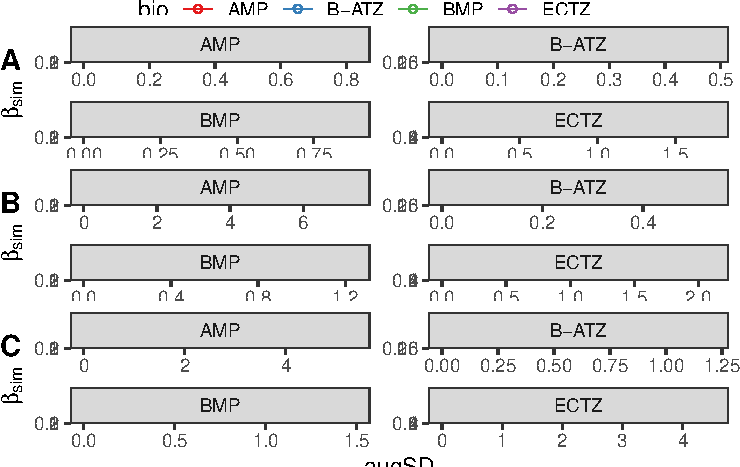
\includegraphics[keepaspectratio]{index_files/mediabag/multiple_linear_regression_files/figure-pdf/fig-mlr6-1.pdf}}

}

\caption{\label{fig-mlr6}Individual linear regression fit to the
variables \texttt{augMean}, \texttt{febSD}, and \texttt{augSD} for each
bioregion as predictors of the seaweed species composition.}

\end{figure}%

\section{Alternative Categorical Variable Coding Schemes
(Contrasts)}\label{sec-contrasts}

Throughout the book, we have used dummy variable coding the specify the
categorical variables in the multiple linear regression models. But,
should dummy variable coding not be to your liking, there are other
coding schemes that can be used to represent the categorical variables.
These alternative coding schemes are known as contrasts. The choice of
contrast coding can affect the interpretation of the regression
coefficients.

I'll provide some synthetic data to illustrate a few different
contrasts. The data consist of a continuous variable \texttt{x}, a
categorical variable \texttt{cat\_var} with four levels, and a response
variable \texttt{y} that has some relationship with \texttt{x} and
\texttt{cat\_var}. I'll use dummy variable coding as the reference
(haha!).

\begin{Shaded}
\begin{Highlighting}[]
\FunctionTok{head}\NormalTok{(data)}
\SpecialCharTok{\textgreater{}}\NormalTok{            y           x cat\_var}
\SpecialCharTok{\textgreater{}} \DecValTok{1}  \FloatTok{0.6667876} \SpecialCharTok{{-}}\FloatTok{0.56047565}\NormalTok{       B}
\SpecialCharTok{\textgreater{}} \DecValTok{2}  \FloatTok{1.3086873} \SpecialCharTok{{-}}\FloatTok{0.23017749}\NormalTok{       B}
\SpecialCharTok{\textgreater{}} \DecValTok{3}  \FloatTok{0.4496192}  \FloatTok{1.55870831}\NormalTok{       D}
\SpecialCharTok{\textgreater{}} \DecValTok{4}  \FloatTok{2.1326402}  \FloatTok{0.07050839}\NormalTok{       A}
\SpecialCharTok{\textgreater{}} \DecValTok{5} \SpecialCharTok{{-}}\FloatTok{2.8608771}  \FloatTok{0.12928774}\NormalTok{       D}
\SpecialCharTok{\textgreater{}} \DecValTok{6}  \FloatTok{0.1497346}  \FloatTok{1.71506499}\NormalTok{       D}
\end{Highlighting}
\end{Shaded}

Categorical variable coding (any scheme) only affects the interpretation
of the categorical variable main effects and their interactions, so I'll
not discuss the coefficient associated with the continuous variable
\texttt{x} (the slope) in the model throughout the explanations offered
below.

\textbf{Dummy Variable Coding (Treatment Contrasts)}

This is the most commonly used coding scheme, and \texttt{lm()}'s
default. One level is the reference category (\texttt{A}) and the other
levels are compared against it. Contrast matrices can be assigned and/or
inspected using the \texttt{contrasts()} function. For the dummy coding,
the reference level \texttt{A} will remain 0 and the other levels will
be independently coded as 1 in three columns. You'll now understand why,
when we have four levels within a categorical variable, we only need
three dummy variables to represent them.

\begin{Shaded}
\begin{Highlighting}[]
\CommentTok{\# Dummy coding (treatment coding) ... default}
\FunctionTok{contrasts}\NormalTok{(data}\SpecialCharTok{$}\NormalTok{cat\_var)}
\SpecialCharTok{\textgreater{}}\NormalTok{   B C D}
\SpecialCharTok{\textgreater{}}\NormalTok{ A }\DecValTok{0} \DecValTok{0} \DecValTok{0}
\SpecialCharTok{\textgreater{}}\NormalTok{ B }\DecValTok{1} \DecValTok{0} \DecValTok{0}
\SpecialCharTok{\textgreater{}}\NormalTok{ C }\DecValTok{0} \DecValTok{1} \DecValTok{0}
\SpecialCharTok{\textgreater{}}\NormalTok{ D }\DecValTok{0} \DecValTok{0} \DecValTok{1}
\end{Highlighting}
\end{Shaded}

When we have four levels in a categorical variable, there are three
dummy variable columns in the contrast matrix. The first row, consisting
of all zeros (0, 0, 0), represents the reference level, which in this
case is \texttt{A}. The other rows represent the different levels of the
categorical variable, with a 1 in the respective column indicating that
level. For example, level \texttt{A} is represented by (0, 0, 0),
\texttt{B} by (1, 0, 0), \texttt{C} by (0, 1, 0), and \texttt{D} by (0,
0, 1). In the regression model, these contrasts are used to estimate the
differences between each level and the reference level. Specifically,
the first contrast column indicates that the coefficient for this column
will represent the difference between the mean of the response variable
for level \texttt{B} and the mean for the reference level \texttt{A},
holding all other variables constant. Similarly, the second and third
columns represent the differences between levels \texttt{C} and
\texttt{A}, and \texttt{D} and \texttt{A}, respectively. This coding
allows for a straightforward interpretation of how each level of the
categorical variable affects the response variable relative to the
reference level.

\begin{Shaded}
\begin{Highlighting}[]
\NormalTok{model\_dummy }\OtherTok{\textless{}{-}} \FunctionTok{lm}\NormalTok{(y }\SpecialCharTok{\textasciitilde{}}\NormalTok{ x }\SpecialCharTok{+}\NormalTok{ cat\_var, }\AttributeTok{data =}\NormalTok{ data)}
\FunctionTok{summary}\NormalTok{(model\_dummy)}
\SpecialCharTok{\textgreater{}} 
\ErrorTok{\textgreater{}}\NormalTok{ Call}\SpecialCharTok{:}
\ErrorTok{\textgreater{}} \FunctionTok{lm}\NormalTok{(}\AttributeTok{formula =}\NormalTok{ y }\SpecialCharTok{\textasciitilde{}}\NormalTok{ x }\SpecialCharTok{+}\NormalTok{ cat\_var, }\AttributeTok{data =}\NormalTok{ data)}
\SpecialCharTok{\textgreater{}} 
\ErrorTok{\textgreater{}}\NormalTok{ Residuals}\SpecialCharTok{:}
\ErrorTok{\textgreater{}}\NormalTok{     Min      }\DecValTok{1}\NormalTok{Q  Median      }\DecValTok{3}\NormalTok{Q     Max }
\SpecialCharTok{\textgreater{}} \SpecialCharTok{{-}}\FloatTok{1.6615} \SpecialCharTok{{-}}\FloatTok{0.6297} \SpecialCharTok{{-}}\FloatTok{0.1494}  \FloatTok{0.4978}  \FloatTok{2.9305} 
\SpecialCharTok{\textgreater{}} 
\ErrorTok{\textgreater{}}\NormalTok{ Coefficients}\SpecialCharTok{:}
\ErrorTok{\textgreater{}}\NormalTok{             Estimate Std. Error t value }\FunctionTok{Pr}\NormalTok{(}\SpecialCharTok{\textgreater{}}\ErrorTok{|}\NormalTok{t}\SpecialCharTok{|}\NormalTok{)    }
\SpecialCharTok{\textgreater{}}\NormalTok{ (Intercept)   }\FloatTok{2.8176}     \FloatTok{0.1635}  \FloatTok{17.232}  \SpecialCharTok{\textless{}} \FloatTok{2e{-}16} \SpecialCharTok{**}\ErrorTok{*}
\ErrorTok{\textgreater{}}\NormalTok{ x             }\FloatTok{1.8274}     \FloatTok{0.1040}  \FloatTok{17.572}  \SpecialCharTok{\textless{}} \FloatTok{2e{-}16} \SpecialCharTok{**}\ErrorTok{*}
\ErrorTok{\textgreater{}}\NormalTok{ cat\_varB     }\SpecialCharTok{{-}}\FloatTok{1.7201}     \FloatTok{0.2499}  \SpecialCharTok{{-}}\FloatTok{6.883} \FloatTok{6.24e{-}10} \SpecialCharTok{**}\ErrorTok{*}
\ErrorTok{\textgreater{}}\NormalTok{ cat\_varC     }\SpecialCharTok{{-}}\FloatTok{3.9056}     \FloatTok{0.2678} \SpecialCharTok{{-}}\FloatTok{14.586}  \SpecialCharTok{\textless{}} \FloatTok{2e{-}16} \SpecialCharTok{**}\ErrorTok{*}
\ErrorTok{\textgreater{}}\NormalTok{ cat\_varD     }\SpecialCharTok{{-}}\FloatTok{5.4880}     \FloatTok{0.2512} \SpecialCharTok{{-}}\FloatTok{21.850}  \SpecialCharTok{\textless{}} \FloatTok{2e{-}16} \SpecialCharTok{**}\ErrorTok{*}
\ErrorTok{\textgreater{}} \SpecialCharTok{{-}{-}{-}}
\ErrorTok{\textgreater{}}\NormalTok{ Signif. codes}\SpecialCharTok{:}  \DecValTok{0} \StringTok{\textquotesingle{}***\textquotesingle{}} \FloatTok{0.001} \StringTok{\textquotesingle{}**\textquotesingle{}} \FloatTok{0.01} \StringTok{\textquotesingle{}*\textquotesingle{}} \FloatTok{0.05} \StringTok{\textquotesingle{}.\textquotesingle{}} \FloatTok{0.1} \StringTok{\textquotesingle{} \textquotesingle{}} \DecValTok{1}
\SpecialCharTok{\textgreater{}} 
\ErrorTok{\textgreater{}}\NormalTok{ Residual standard error}\SpecialCharTok{:} \FloatTok{0.9246}\NormalTok{ on }\DecValTok{95}\NormalTok{ degrees of freedom}
\SpecialCharTok{\textgreater{}}\NormalTok{ Multiple R}\SpecialCharTok{{-}}\NormalTok{squared}\SpecialCharTok{:}  \FloatTok{0.887}\NormalTok{,   Adjusted R}\SpecialCharTok{{-}}\NormalTok{squared}\SpecialCharTok{:}  \FloatTok{0.8822} 
\SpecialCharTok{\textgreater{}}\NormalTok{ F}\SpecialCharTok{{-}}\NormalTok{statistic}\SpecialCharTok{:} \FloatTok{186.4}\NormalTok{ on }\DecValTok{4}\NormalTok{ and }\DecValTok{95}\NormalTok{ DF,  p}\SpecialCharTok{{-}}\NormalTok{value}\SpecialCharTok{:} \ErrorTok{\textless{}} \FloatTok{2.2e{-}16}
\end{Highlighting}
\end{Shaded}

The model summary shows that the coefficients for \texttt{cat\_varB},
\texttt{cat\_varC}, and \texttt{cat\_varD} represent the differences in
the mean of the response variable \texttt{y} between the reference
category \texttt{A} and categories \texttt{B}, \texttt{C}, and
\texttt{D}, respectively, while controlling for the effect of the
continuous variable \texttt{x}.

Interpretation:

\begin{itemize}
\tightlist
\item
  \texttt{(Intercept)} (2.8176): The intercept represents the estimated
  mean value of the response (\texttt{y}) when \texttt{x} is zero and
  the categorical variable is at the reference level \texttt{A}. This is
  the baseline from which other categories are compared.
\item
  \texttt{x} (1.8274): For each one-unit increase in \texttt{x},
  \texttt{y} is expected to increase by 1.8274 units, holding the
  categorical variable constant. This effect is consistent across all
  levels of the categorical variable because the model does not have an
  interaction effect present.
\item
  \texttt{cat\_varB} (-1.7201): On average, the value of \texttt{y} for
  level \texttt{B} is 1.7201 units lower than that for the reference
  level \texttt{A}, when \texttt{x} is held constant. This corresponds
  to the (1, 0, 0) row in the contrast matrix.
\item
  \texttt{cat\_varC} (-3.9056): Similarly, on average, the value of
  \texttt{y} for level \texttt{C} is 3.9056 units lower than that for
  the reference level, when \texttt{x} is held constant. This
  corresponds to the (0, 1, 0) row in the contrast matrix.
\item
  \texttt{cat\_varD} (-5.4880): Lastly, on average, the value of
  \texttt{y} for level \texttt{D} is 5.4880 units lower compared to the
  reference , when \texttt{x} is held constant. This is row (0, 0, 1)
  row in the contrast matrix.
\end{itemize}

All these coefficients are highly significant (\emph{p} \textless{}
0.0001), indicating strong evidence for differences between each
category and the reference category \texttt{A}.

The model explains a large proportion of the variance in \texttt{y}
(Adjusted \emph{R}-squared: 0.8822), suggesting a good fit. The
\emph{F}-statistic (186.4) with a very low \emph{p}-value (\textless{}
0.0001) indicates that the model as a whole is statistically
significant.

If you want to change the reference level, you can use the
\texttt{relevel()} function. For example, to change the reference level
of \texttt{cat\_var} variable to \texttt{C\_2}, you can use:

\begin{Shaded}
\begin{Highlighting}[]
\CommentTok{\# Set "C" as the reference level for cat\_var}
\NormalTok{data}\SpecialCharTok{$}\NormalTok{cat\_var }\OtherTok{\textless{}{-}} \FunctionTok{relevel}\NormalTok{(data}\SpecialCharTok{$}\NormalTok{cat\_var, }\AttributeTok{ref =} \StringTok{"C"}\NormalTok{)}
\FunctionTok{contrasts}\NormalTok{(data}\SpecialCharTok{$}\NormalTok{cat\_var)}
\SpecialCharTok{\textgreater{}}\NormalTok{   A B D}
\SpecialCharTok{\textgreater{}}\NormalTok{ C }\DecValTok{0} \DecValTok{0} \DecValTok{0}
\SpecialCharTok{\textgreater{}}\NormalTok{ A }\DecValTok{1} \DecValTok{0} \DecValTok{0}
\SpecialCharTok{\textgreater{}}\NormalTok{ B }\DecValTok{0} \DecValTok{1} \DecValTok{0}
\SpecialCharTok{\textgreater{}}\NormalTok{ D }\DecValTok{0} \DecValTok{0} \DecValTok{1}
\end{Highlighting}
\end{Shaded}

This may be useful when you want to compare the other levels to a
different reference level.

\textbf{Effect Coding (Sum Contrasts)}

This coding method compares the levels of a categorical variable to the
overall mean of the dependent variable. The coefficients represent the
difference between each level and the grand mean. Instead of using 0 and
1 as we did with dummy variable coding, effect coding uses -1, 0, and 1
to represent the different levels of the categorical variable.

\begin{Shaded}
\begin{Highlighting}[]
\CommentTok{\# Reset the reference level to "A"}
\NormalTok{data }\OtherTok{\textless{}{-}} \FunctionTok{data.frame}\NormalTok{(y, x, cat\_var)}

\CommentTok{\# Effect coding}
\FunctionTok{contrasts}\NormalTok{(data}\SpecialCharTok{$}\NormalTok{cat\_var) }\OtherTok{\textless{}{-}} \FunctionTok{contr.sum}\NormalTok{(}\DecValTok{4}\NormalTok{)}
\FunctionTok{contrasts}\NormalTok{(data}\SpecialCharTok{$}\NormalTok{cat\_var)}
\SpecialCharTok{\textgreater{}}\NormalTok{   [,}\DecValTok{1}\NormalTok{] [,}\DecValTok{2}\NormalTok{] [,}\DecValTok{3}\NormalTok{]}
\SpecialCharTok{\textgreater{}}\NormalTok{ A    }\DecValTok{1}    \DecValTok{0}    \DecValTok{0}
\SpecialCharTok{\textgreater{}}\NormalTok{ B    }\DecValTok{0}    \DecValTok{1}    \DecValTok{0}
\SpecialCharTok{\textgreater{}}\NormalTok{ C    }\DecValTok{0}    \DecValTok{0}    \DecValTok{1}
\SpecialCharTok{\textgreater{}}\NormalTok{ D   }\SpecialCharTok{{-}}\DecValTok{1}   \SpecialCharTok{{-}}\DecValTok{1}   \SpecialCharTok{{-}}\DecValTok{1}
\end{Highlighting}
\end{Shaded}

In effect coding (sum contrasts), each level of the categorical variable
is compared to the overall mean rather than a specific reference
category. This contrast matrix with four levels (A, B, C, D) and three
columns can be interpreted as follows:

\begin{itemize}
\tightlist
\item
  Level \texttt{A} (1, 0, 0): The first row indicates that level
  \texttt{A} is included in the first contrast (\texttt{cat\_var1}),
  which means the mean of level \texttt{A} is being compared to the
  overall mean. Since the other columns are zero, level \texttt{A} does
  not contribute to the other contrasts.
\item
  Level \texttt{B} (0, 1, 0): The second row indicates that level
  \texttt{B} is included in the second contrast (\texttt{cat\_var2}).
  The mean of level \texttt{B} is being compared to the overall mean,
  and it does not contribute to the other contrasts.
\item
  Level \texttt{C} (0, 0, 1): The third row indicates that level
  \texttt{C} is included in the third contrast (\texttt{cat\_var3}). The
  mean of level C is being compared to the overall mean, and it does not
  contribute to the other contrasts.
\item
  Level \texttt{D} (-1, -1, -1): The fourth row is a balancing row,
  ensuring that the sum of the contrasts for each level equals zero.
  This indicates that level D is being compared to the overall mean
  indirectly by balancing the contributions of levels \texttt{A},
  \texttt{B}, and \texttt{C}.
\end{itemize}

\begin{Shaded}
\begin{Highlighting}[]
\NormalTok{model\_effect }\OtherTok{\textless{}{-}} \FunctionTok{lm}\NormalTok{(y }\SpecialCharTok{\textasciitilde{}}\NormalTok{ x }\SpecialCharTok{+}\NormalTok{ cat\_var, }\AttributeTok{data =}\NormalTok{ data)}
\FunctionTok{summary}\NormalTok{(model\_effect)}
\SpecialCharTok{\textgreater{}} 
\ErrorTok{\textgreater{}}\NormalTok{ Call}\SpecialCharTok{:}
\ErrorTok{\textgreater{}} \FunctionTok{lm}\NormalTok{(}\AttributeTok{formula =}\NormalTok{ y }\SpecialCharTok{\textasciitilde{}}\NormalTok{ x }\SpecialCharTok{+}\NormalTok{ cat\_var, }\AttributeTok{data =}\NormalTok{ data)}
\SpecialCharTok{\textgreater{}} 
\ErrorTok{\textgreater{}}\NormalTok{ Residuals}\SpecialCharTok{:}
\ErrorTok{\textgreater{}}\NormalTok{     Min      }\DecValTok{1}\NormalTok{Q  Median      }\DecValTok{3}\NormalTok{Q     Max }
\SpecialCharTok{\textgreater{}} \SpecialCharTok{{-}}\FloatTok{1.6615} \SpecialCharTok{{-}}\FloatTok{0.6297} \SpecialCharTok{{-}}\FloatTok{0.1494}  \FloatTok{0.4978}  \FloatTok{2.9305} 
\SpecialCharTok{\textgreater{}} 
\ErrorTok{\textgreater{}}\NormalTok{ Coefficients}\SpecialCharTok{:}
\ErrorTok{\textgreater{}}\NormalTok{             Estimate Std. Error t value }\FunctionTok{Pr}\NormalTok{(}\SpecialCharTok{\textgreater{}}\ErrorTok{|}\NormalTok{t}\SpecialCharTok{|}\NormalTok{)    }
\SpecialCharTok{\textgreater{}}\NormalTok{ (Intercept)  }\FloatTok{0.03921}    \FloatTok{0.09452}   \FloatTok{0.415}    \FloatTok{0.679}    
\SpecialCharTok{\textgreater{}}\NormalTok{ x            }\FloatTok{1.82741}    \FloatTok{0.10400}  \FloatTok{17.572}  \SpecialCharTok{\textless{}} \FloatTok{2e{-}16} \SpecialCharTok{**}\ErrorTok{*}
\ErrorTok{\textgreater{}}\NormalTok{ cat\_var1     }\FloatTok{2.77844}    \FloatTok{0.14968}  \FloatTok{18.563}  \SpecialCharTok{\textless{}} \FloatTok{2e{-}16} \SpecialCharTok{**}\ErrorTok{*}
\ErrorTok{\textgreater{}}\NormalTok{ cat\_var2     }\FloatTok{1.05832}    \FloatTok{0.16329}   \FloatTok{6.481} \FloatTok{4.04e{-}09} \SpecialCharTok{**}\ErrorTok{*}
\ErrorTok{\textgreater{}}\NormalTok{ cat\_var3    }\SpecialCharTok{{-}}\FloatTok{1.12720}    \FloatTok{0.17765}  \SpecialCharTok{{-}}\FloatTok{6.345} \FloatTok{7.53e{-}09} \SpecialCharTok{**}\ErrorTok{*}
\ErrorTok{\textgreater{}} \SpecialCharTok{{-}{-}{-}}
\ErrorTok{\textgreater{}}\NormalTok{ Signif. codes}\SpecialCharTok{:}  \DecValTok{0} \StringTok{\textquotesingle{}***\textquotesingle{}} \FloatTok{0.001} \StringTok{\textquotesingle{}**\textquotesingle{}} \FloatTok{0.01} \StringTok{\textquotesingle{}*\textquotesingle{}} \FloatTok{0.05} \StringTok{\textquotesingle{}.\textquotesingle{}} \FloatTok{0.1} \StringTok{\textquotesingle{} \textquotesingle{}} \DecValTok{1}
\SpecialCharTok{\textgreater{}} 
\ErrorTok{\textgreater{}}\NormalTok{ Residual standard error}\SpecialCharTok{:} \FloatTok{0.9246}\NormalTok{ on }\DecValTok{95}\NormalTok{ degrees of freedom}
\SpecialCharTok{\textgreater{}}\NormalTok{ Multiple R}\SpecialCharTok{{-}}\NormalTok{squared}\SpecialCharTok{:}  \FloatTok{0.887}\NormalTok{,   Adjusted R}\SpecialCharTok{{-}}\NormalTok{squared}\SpecialCharTok{:}  \FloatTok{0.8822} 
\SpecialCharTok{\textgreater{}}\NormalTok{ F}\SpecialCharTok{{-}}\NormalTok{statistic}\SpecialCharTok{:} \FloatTok{186.4}\NormalTok{ on }\DecValTok{4}\NormalTok{ and }\DecValTok{95}\NormalTok{ DF,  p}\SpecialCharTok{{-}}\NormalTok{value}\SpecialCharTok{:} \ErrorTok{\textless{}} \FloatTok{2.2e{-}16}
\end{Highlighting}
\end{Shaded}

Interpretation:

\begin{itemize}
\tightlist
\item
  \texttt{(Intercept)} 0.03921: The intercept represents the grand mean
  of the response variable (\texttt{y}). Since the intercept is not
  statistically significant (\emph{p} \textgreater{} 0.05), it indicates
  that the overall mean is not significantly different from zero when
  considering the average effect of all levels of the categorical
  variable.
\item
  \texttt{x} (1.82741): For each one-unit increase in (\texttt{x}), the
  response (\texttt{y}) increases by approximately 1.82741 units. This
  effect is highly significant (\emph{p} \textless{} 0.0001).
\item
  \texttt{cat\_var1} (2.77844): Level \texttt{A} has a mean (\texttt{y})
  that is 2.77844 units higher than the grand mean. This effect is
  highly significant (\emph{p} \textless{} 0.0001).
\item
  \texttt{cat\_var2} (1.05832): Level \texttt{B} has a mean (\texttt{y})
  that is 1.05832 units higher than the grand mean. This effect is also
  highly significant (\emph{p} \textless{} 0.0001).
\item
  \texttt{cat\_var3} (-1.12720): Level \texttt{C} has a mean
  (\texttt{y}) that is 1.12720 units lower than the grand mean. This
  effect is highly significant (p \textless{} 0.0001).
\end{itemize}

All these coefficients are highly significant (\emph{p} \textless{}
0.0001), indicating strong evidence for differences between each
category and the overall mean of all levels.

The model explains a large proportion of the variance in \texttt{y}
(Adjusted \emph{R}-squared: 0.8822), suggesting a good fit. The
\emph{F}-statistic (186.4) with a very low \emph{p}-value (\textless{}
0.0001) indicates that the model as a whole is statistically
significant.

\textbf{Helmert Coding}

Helmert coding compares each level of a categorical variable to the mean
of the subsequent levels. It is useful for testing ordered differences.

\begin{Shaded}
\begin{Highlighting}[]
\CommentTok{\# Helmert coding}
\FunctionTok{contrasts}\NormalTok{(data}\SpecialCharTok{$}\NormalTok{cat\_var) }\OtherTok{\textless{}{-}} \FunctionTok{contr.helmert}\NormalTok{(}\DecValTok{4}\NormalTok{)}
\FunctionTok{contrasts}\NormalTok{(data}\SpecialCharTok{$}\NormalTok{cat\_var)}
\SpecialCharTok{\textgreater{}}\NormalTok{   [,}\DecValTok{1}\NormalTok{] [,}\DecValTok{2}\NormalTok{] [,}\DecValTok{3}\NormalTok{]}
\SpecialCharTok{\textgreater{}}\NormalTok{ A   }\SpecialCharTok{{-}}\DecValTok{1}   \SpecialCharTok{{-}}\DecValTok{1}   \SpecialCharTok{{-}}\DecValTok{1}
\SpecialCharTok{\textgreater{}}\NormalTok{ B    }\DecValTok{1}   \SpecialCharTok{{-}}\DecValTok{1}   \SpecialCharTok{{-}}\DecValTok{1}
\SpecialCharTok{\textgreater{}}\NormalTok{ C    }\DecValTok{0}    \DecValTok{2}   \SpecialCharTok{{-}}\DecValTok{1}
\SpecialCharTok{\textgreater{}}\NormalTok{ D    }\DecValTok{0}    \DecValTok{0}    \DecValTok{3}
\end{Highlighting}
\end{Shaded}

The contrast matrix for a categorical variable with four levels
(\texttt{A}, \texttt{B}, \texttt{C}, \texttt{D}) and three columns can
be interpreted as follows:

\begin{itemize}
\tightlist
\item
  Level \texttt{A} (-1, -1, -1): Level \texttt{A} is compared to the
  mean of levels \texttt{B}, \texttt{C}, and \texttt{D}. The negative
  values indicate that level A is being subtracted in these comparisons.
\item
  Level \texttt{B} (1, -1, -1): Level \texttt{B} is compared to the mean
  of levels \texttt{C} and \texttt{D}. The positive value in the first
  column indicates that level \texttt{B} is being added in this
  comparison.
\item
  Level \texttt{C} (0, 2, -1): Level \texttt{C} is compared to the mean
  of level \texttt{D}. The positive value in the second column indicates
  that level \texttt{C} is being added in this comparison, while the
  negative value in the third column is part of the comparison for
  subsequent levels.
\item
  Level \texttt{D} (0, 0, 3): Level \texttt{D} is compared on its own in
  the final contrast. The positive value in the third column indicates
  that level \texttt{D} is being added in this comparison.
\end{itemize}

\begin{Shaded}
\begin{Highlighting}[]
\NormalTok{model\_helmert }\OtherTok{\textless{}{-}} \FunctionTok{lm}\NormalTok{(y }\SpecialCharTok{\textasciitilde{}}\NormalTok{ x }\SpecialCharTok{+}\NormalTok{ cat\_var, }\AttributeTok{data =}\NormalTok{ data)}
\FunctionTok{summary}\NormalTok{(model\_helmert)}
\SpecialCharTok{\textgreater{}} 
\ErrorTok{\textgreater{}}\NormalTok{ Call}\SpecialCharTok{:}
\ErrorTok{\textgreater{}} \FunctionTok{lm}\NormalTok{(}\AttributeTok{formula =}\NormalTok{ y }\SpecialCharTok{\textasciitilde{}}\NormalTok{ x }\SpecialCharTok{+}\NormalTok{ cat\_var, }\AttributeTok{data =}\NormalTok{ data)}
\SpecialCharTok{\textgreater{}} 
\ErrorTok{\textgreater{}}\NormalTok{ Residuals}\SpecialCharTok{:}
\ErrorTok{\textgreater{}}\NormalTok{     Min      }\DecValTok{1}\NormalTok{Q  Median      }\DecValTok{3}\NormalTok{Q     Max }
\SpecialCharTok{\textgreater{}} \SpecialCharTok{{-}}\FloatTok{1.6615} \SpecialCharTok{{-}}\FloatTok{0.6297} \SpecialCharTok{{-}}\FloatTok{0.1494}  \FloatTok{0.4978}  \FloatTok{2.9305} 
\SpecialCharTok{\textgreater{}} 
\ErrorTok{\textgreater{}}\NormalTok{ Coefficients}\SpecialCharTok{:}
\ErrorTok{\textgreater{}}\NormalTok{             Estimate Std. Error t value }\FunctionTok{Pr}\NormalTok{(}\SpecialCharTok{\textgreater{}}\ErrorTok{|}\NormalTok{t}\SpecialCharTok{|}\NormalTok{)    }
\SpecialCharTok{\textgreater{}}\NormalTok{ (Intercept)  }\FloatTok{0.03921}    \FloatTok{0.09452}   \FloatTok{0.415}    \FloatTok{0.679}    
\SpecialCharTok{\textgreater{}}\NormalTok{ x            }\FloatTok{1.82741}    \FloatTok{0.10400}  \FloatTok{17.572}  \SpecialCharTok{\textless{}} \FloatTok{2e{-}16} \SpecialCharTok{**}\ErrorTok{*}
\ErrorTok{\textgreater{}}\NormalTok{ cat\_var1    }\SpecialCharTok{{-}}\FloatTok{0.86006}    \FloatTok{0.12495}  \SpecialCharTok{{-}}\FloatTok{6.883} \FloatTok{6.24e{-}10} \SpecialCharTok{**}\ErrorTok{*}
\ErrorTok{\textgreater{}}\NormalTok{ cat\_var2    }\SpecialCharTok{{-}}\FloatTok{1.01519}    \FloatTok{0.08206} \SpecialCharTok{{-}}\FloatTok{12.371}  \SpecialCharTok{\textless{}} \FloatTok{2e{-}16} \SpecialCharTok{**}\ErrorTok{*}
\ErrorTok{\textgreater{}}\NormalTok{ cat\_var3    }\SpecialCharTok{{-}}\FloatTok{0.90319}    \FloatTok{0.05477} \SpecialCharTok{{-}}\FloatTok{16.491}  \SpecialCharTok{\textless{}} \FloatTok{2e{-}16} \SpecialCharTok{**}\ErrorTok{*}
\ErrorTok{\textgreater{}} \SpecialCharTok{{-}{-}{-}}
\ErrorTok{\textgreater{}}\NormalTok{ Signif. codes}\SpecialCharTok{:}  \DecValTok{0} \StringTok{\textquotesingle{}***\textquotesingle{}} \FloatTok{0.001} \StringTok{\textquotesingle{}**\textquotesingle{}} \FloatTok{0.01} \StringTok{\textquotesingle{}*\textquotesingle{}} \FloatTok{0.05} \StringTok{\textquotesingle{}.\textquotesingle{}} \FloatTok{0.1} \StringTok{\textquotesingle{} \textquotesingle{}} \DecValTok{1}
\SpecialCharTok{\textgreater{}} 
\ErrorTok{\textgreater{}}\NormalTok{ Residual standard error}\SpecialCharTok{:} \FloatTok{0.9246}\NormalTok{ on }\DecValTok{95}\NormalTok{ degrees of freedom}
\SpecialCharTok{\textgreater{}}\NormalTok{ Multiple R}\SpecialCharTok{{-}}\NormalTok{squared}\SpecialCharTok{:}  \FloatTok{0.887}\NormalTok{,   Adjusted R}\SpecialCharTok{{-}}\NormalTok{squared}\SpecialCharTok{:}  \FloatTok{0.8822} 
\SpecialCharTok{\textgreater{}}\NormalTok{ F}\SpecialCharTok{{-}}\NormalTok{statistic}\SpecialCharTok{:} \FloatTok{186.4}\NormalTok{ on }\DecValTok{4}\NormalTok{ and }\DecValTok{95}\NormalTok{ DF,  p}\SpecialCharTok{{-}}\NormalTok{value}\SpecialCharTok{:} \ErrorTok{\textless{}} \FloatTok{2.2e{-}16}
\end{Highlighting}
\end{Shaded}

Interpretation:

\begin{itemize}
\tightlist
\item
  \texttt{(Intercept)} (0.03921): The grand mean of \texttt{y} when
  \texttt{x} is zero.
\item
  \texttt{x} (1.82741): For each unit increase in x , y increases by
  1.82741 units.
\item
  \texttt{cat\_var1} (-0.86006): The mean of level \texttt{A} is 0.86006
  units lower than the combined mean of levels \texttt{B}, \texttt{C},
  and \texttt{D}.
\item
  \texttt{cat\_var2} (-1.01519): The mean of level \texttt{B} is 1.01519
  units lower than the combined mean of levels \texttt{C} and
  \texttt{D}.
\item
  \texttt{cat\_var3} (-0.90319): The mean of level \texttt{C} is 0.90319
  units lower than the mean of level \texttt{D}.
\end{itemize}

The interpretation of the overall model remains more-or-less similar to
before:

All these coefficients are highly significant (\emph{p} \textless{}
0.0001), indicating strong evidence for differences between each level
and the overall mean of all subsequent levels.

The model explains a large proportion of the variance in \texttt{y}
(Adjusted \emph{R}-squared: 0.8822), suggesting a good fit. The
\emph{F}-statistic (186.4) with a very low \emph{p}-value (\textless{}
0.0001) indicates that the model as a whole is statistically
significant.

\section{Exercises}\label{exercises}

\begin{tcolorbox}[enhanced jigsaw, opacitybacktitle=0.6, toptitle=1mm, colframe=quarto-callout-important-color-frame, arc=.35mm, left=2mm, rightrule=.15mm, coltitle=black, opacityback=0, bottomrule=.15mm, bottomtitle=1mm, title=\textcolor{quarto-callout-important-color}{\faExclamation}\hspace{0.5em}{Task G}, toprule=.15mm, colbacktitle=quarto-callout-important-color!10!white, titlerule=0mm, leftrule=.75mm, colback=white, breakable]

Use the data loaded at the start of this chapter for this task.

In this task you will develop data analysis, undertake model building,
and provide an interpretation of the findings. Your goal is to explore
the species composition and assembly processes of the seaweed flora
around the coast of South Africa. See {[}3{]} for more information about
the data and the analysis.

\begin{enumerate}
\def\labelenumi{\alph{enumi}.}
\item
  \textbf{Analysis:} Please develop multiple linear regression models
  for the seaweed species composition (\(\beta_\text{sim}\) and
  \(\beta_\text{sne}\), i.e.~columns called \texttt{Y1} and \texttt{Y2},
  respectively) using the all the predictors in this dataset. At the
  end, the final model(s) that best describe(s) the species assembly
  processes operating along the South African coast should be presented.
  The final model may/may not contain all the predictors in the dataset,
  and it is your goal to justify the variable and model selection.

  \begin{itemize}
  \tightlist
  \item
    Accomplishing a) will require that you work through the whole
    model-building process as outlined in the chapter. This includes the
    following steps:

    \begin{itemize}
    \tightlist
    \item
      Data exploration and visualisation (EDA)
    \item
      Model building (providing hypothesis statements, variable
      selection using VIF and forward selection, comparisons of nested
      models, justifications for model selection)
    \item
      Model diagnostics
    \item
      Explanation of \texttt{summary()} and \texttt{anova()} outputs
    \item
      Producing the Results section
    \item
      \textbf{{[}60\%{]}}
    \end{itemize}
  \end{itemize}
\item
  \textbf{Interpretation:} Once you have arrived at the best model,
  discuss your findings in the light of the appropriate ecological
  hypotheses that explain the relationships between the predictors and
  the seaweed species composition. Include insights drawn from the
  analysis of \(\beta_\text{sør}\) that I developed in this chapter, and
  also rely on the theory you have developed for the lecture material
  the class presented in Task A2.

  \begin{itemize}
  \tightlist
  \item
    Accomplishing b) is thus all about model interpretation and
    discussing the ecological relevance of the results.
  \item
    \textbf{{[}40\%{]}}
  \end{itemize}
\end{enumerate}

The format of this task is a Quarto file that will be converted to an
HTML file. The HTML file will contain the graphs, all calculations, and
the text sections. The task should be written up as a publication
(i.e.~use appropriate headings) using a journal style of your choice.
Aside from this, there are no limitations.

\end{tcolorbox}

\chapter{Generalised Linear Models
(GLM)}\label{sec-generalised-linear-model}

\section{Logistic Regression}\label{logistic-regression}

A logistic regression model is used when the dependent variable is
binary (e.g., 0 or 1, yes or no). The logistic regression model is
expressed as:

\begin{equation}\phantomsection\label{eq-logit}{\log\left(\frac{p}{1-p}\right) = \alpha + \beta_1 X_{i1} + \beta_2 X_{i2} + \ldots + \beta_k X_{ik}}\end{equation}

Where:

\begin{itemize}
\tightlist
\item
  \(p\) is the probability of the dependent variable being 1,
\item
  \(X_{i1}, X_{i2}, \ldots, X_{ik}\) are the \(k\) predictor variables
  for the \(i\)-th observation,
\item
  \(\alpha\) is the intercept,
\item
  \(\beta_1, \beta_2, \ldots, \beta_k\) are the coefficients for the
  \(k\) predictor variables.
\end{itemize}

\chapter{Nonlinear Models}\label{sec-nonlinear-regression}

Nonlinear regression models\index{nonlinear regression} are used when
the relationship between the response variable (dependent variable,
\(Y\)) and the predictor variables (independent variables, \(X\)) is not
linear. In other words, they are employed when a straight line is not an
appropriate representation of the relationship between the variables.

As we have seen in Section~\ref{sec-simple-linear-regression},
polynomial regressions provide a nonlinear relationship between the
response and predictor variables (as seen in the regression line fit to
the data, Figure~\ref{fig-plts} A), but they are considered linear
models because the parameters are estimated using linear least squares.
Another type of nonlinear model is a semi-parametric model where the
relationship between the response and predictor variables is described
by a function that includes both parametric and non-parametric
components. An example of a semi-parametric model is the generalised
additive model (GAM) that includes a non-parametric component in the
form of a spline function
(Chapter~\ref{sec-generalised-additive-models}; Figure~\ref{fig-plts}
B).

The type of nonlinear model I cover in this chapter is a parametric
model where the relationship between the response and predictor
variables is described by a specific nonlinear function
(Figure~\ref{fig-plts} C). The model still assumes that the residuals
are normally distributed and exhibit homoscedasticity. The model
parameters are estimated by minimising the sum of squared differences
between the observed and predicted values, a method commonly referred to
as nonlinear least squares (NLS) regression. This is the term I will
adopt.

The primary purpose of nonlinear regression is to derive a formula
(model), analyse data, and predict new values where the phenomenon
exhibits a nonlinear causal\index{causal} pattern or behaviour.
Nonlinear models include a variety of response forms, such as
exponential growth models, logistic growth models, and other mechanistic
models derived from physical, chemical, or biological processes.
Examples of such models include trigonometric, logarithmic, and
user-defined functions like the von Bertalanffy model or seasonal cycle
represented by a sine curve (Figure~\ref{fig-plts} C). These models are
explicitly nonlinear in both their form and parameters. Unlike
polynomial regression, where only the terms of \(X\) are transformed,
nonlinear models involve an entirely nonlinear function relating \(X\)
and \(Y\). They are often used when there is a theoretical basis for the
specific form of the relationship, providing interpretable parameters
that carry specific meanings based on the underlying theory, making them
useful for detailed applications where the dynamics of the system are
well-understood.

A general formula for a nonlinear regression model is:

\begin{equation}\phantomsection\label{eq-nonlin}{Y_i = f(X_i; \theta) + \epsilon_i}\end{equation}

Where:

\begin{itemize}
\tightlist
\item
  \(Y_i\) is the response variable for the \(i\)-th observation,
\item
  \(X_i\) is the predictor variable for the \(i\)-th observation,
\item
  \(f(X_i; \theta)\) is a nonlinear function of \(X_i\) parameterised by
  the vector \(\theta\),
\item
  \(\theta\) is the vector of parameters to be estimated, and
\item
  \(\epsilon_i\) is the error term for the \(i\)-th observation and is
  assumed to be i.i.d. with a normal distribution.
\end{itemize}

An example of a specific nonlinear regression model is the exponential
growth model:

\begin{equation}\phantomsection\label{eq-exp}{Y_i = \alpha e^{\beta X_i} + \epsilon_i}\end{equation}

Where:

\begin{itemize}
\tightlist
\item
  \(\alpha\) and \(\beta\) are the parameters to be estimated,
\item
  \(e\) is the base of the natural logarithm, and
\item
  \(\epsilon_i\) is the error term for the \(i\)-th observation.
\end{itemize}

This model is nonlinear in the parameters \(\alpha\) and \(\beta\), and
it describes an exponential relationship between the predictor \(X\) and
the response \(Y\).

\begin{figure}[t]

\centering{

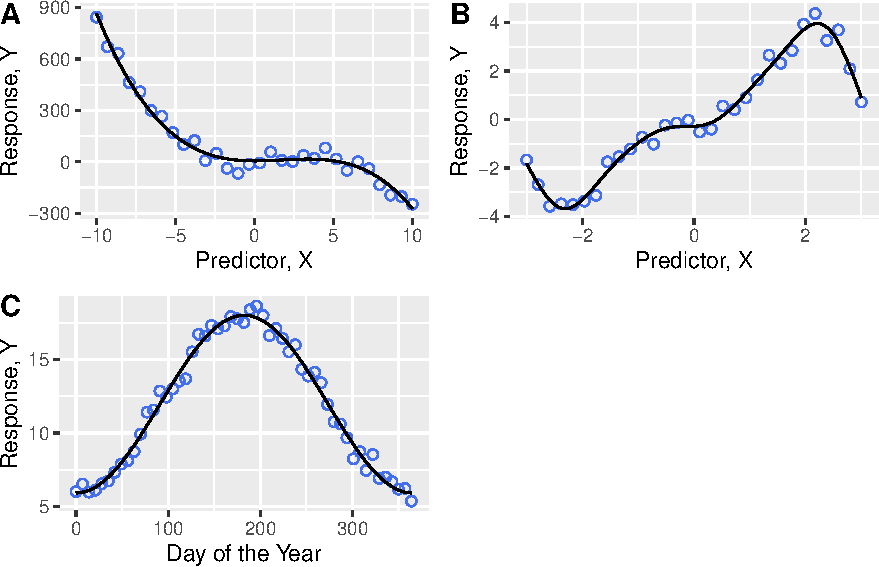
\includegraphics[width=0.8\linewidth,height=\textheight,keepaspectratio]{index_files/mediabag/non-linear_regression_files/figure-pdf/fig-plts-1.pdf}

}

\caption{\label{fig-plts}Nonlinear regression models fitted to simulated
data. A) a cubic polynomial model, B) a GAM with a thin plate regression
spline, and C) a NLS sine curve as a seasonal cycle.}

\end{figure}%

\section{Extension of Nonlinear
Models}\label{extension-of-nonlinear-models}

Like linear models, nonlinear models have also been extended to include
multiple predictors, interactions, and other terms to capture complex
relationships between the variables. The first type of more complex
nonlinear models accommodates a wider range of data distributions by
generalising to non-normal error distributions through link functions.
These models are called generalised nonlinear models (GNLMs). The
examples of GLMs in Chapter~\ref{sec-generalised-linear-model} should
prepare you sufficiently to handle nonlinear models too. The other type
deals with hierarchical data structures and incorporates fixed and
random effects. As such, you can also correctly model repeated measures
and longitudinal, and nested (grouped) designs. These hierarchical
models are called nonlinear mixed models (NLMMs). Examples of NLMMs are
provided in Section~\ref{sec-mf-treatments} and
Section~\ref{sec-perturbation}.

\section{Considerations for Model
Selection}\label{considerations-for-model-selection}

\begin{figure}[t]

\centering{

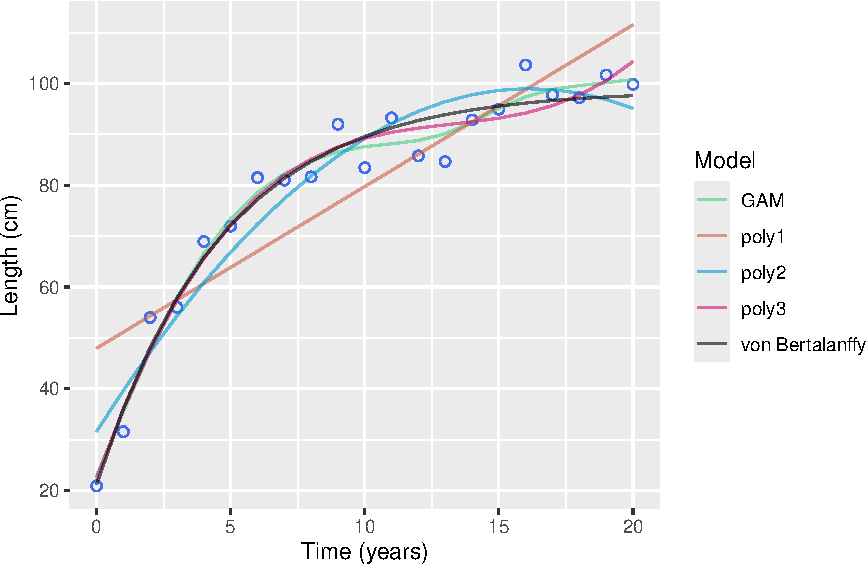
\includegraphics[width=0.8\linewidth,height=\textheight,keepaspectratio]{index_files/mediabag/non-linear_regression_files/figure-pdf/fig-combo-1.pdf}

}

\caption{\label{fig-combo}Plot of growth rate data fitted with a von
Bertalanffy model, a first- (straight line), second- and third-order
polynomial, and a GAM.}

\end{figure}%

There are a few practical considerations to keep in mind when choosing a
suitable nonlinear (in shape) model. Sometimes different models can
provide similar fits to the same data, but they may have different
implications for the interpretation of the relationship between the
variables. See for example Figure~\ref{fig-combo}. The plot shows growth
rate data fitted with a first-, second- and third-order polynomial, a
GAM, and a NLS von Bertalanffy model. To the untrained eye and
inexperienced biologist, all models seem to provide a good fit to the
data, but they do differ subtly in the shape of the fitted curve. The
von Bertalanffy model is a saturating growth model (it reaches a
plateau), while the polynomial models and the GAM are more flexible and
can capture a wider range of shapes. The choice of model should be
guided by the underlying biological or physical processes that generated
the data and the research question you are trying to answer.

Regression analysis will often require that we decide among polynomial
regressions, nonlinear models, GAMs, or some of the more complex
hierarchical models, and there are various considerations to keep in
mind when decising which model to use. I will cover some of these in the
next sections.

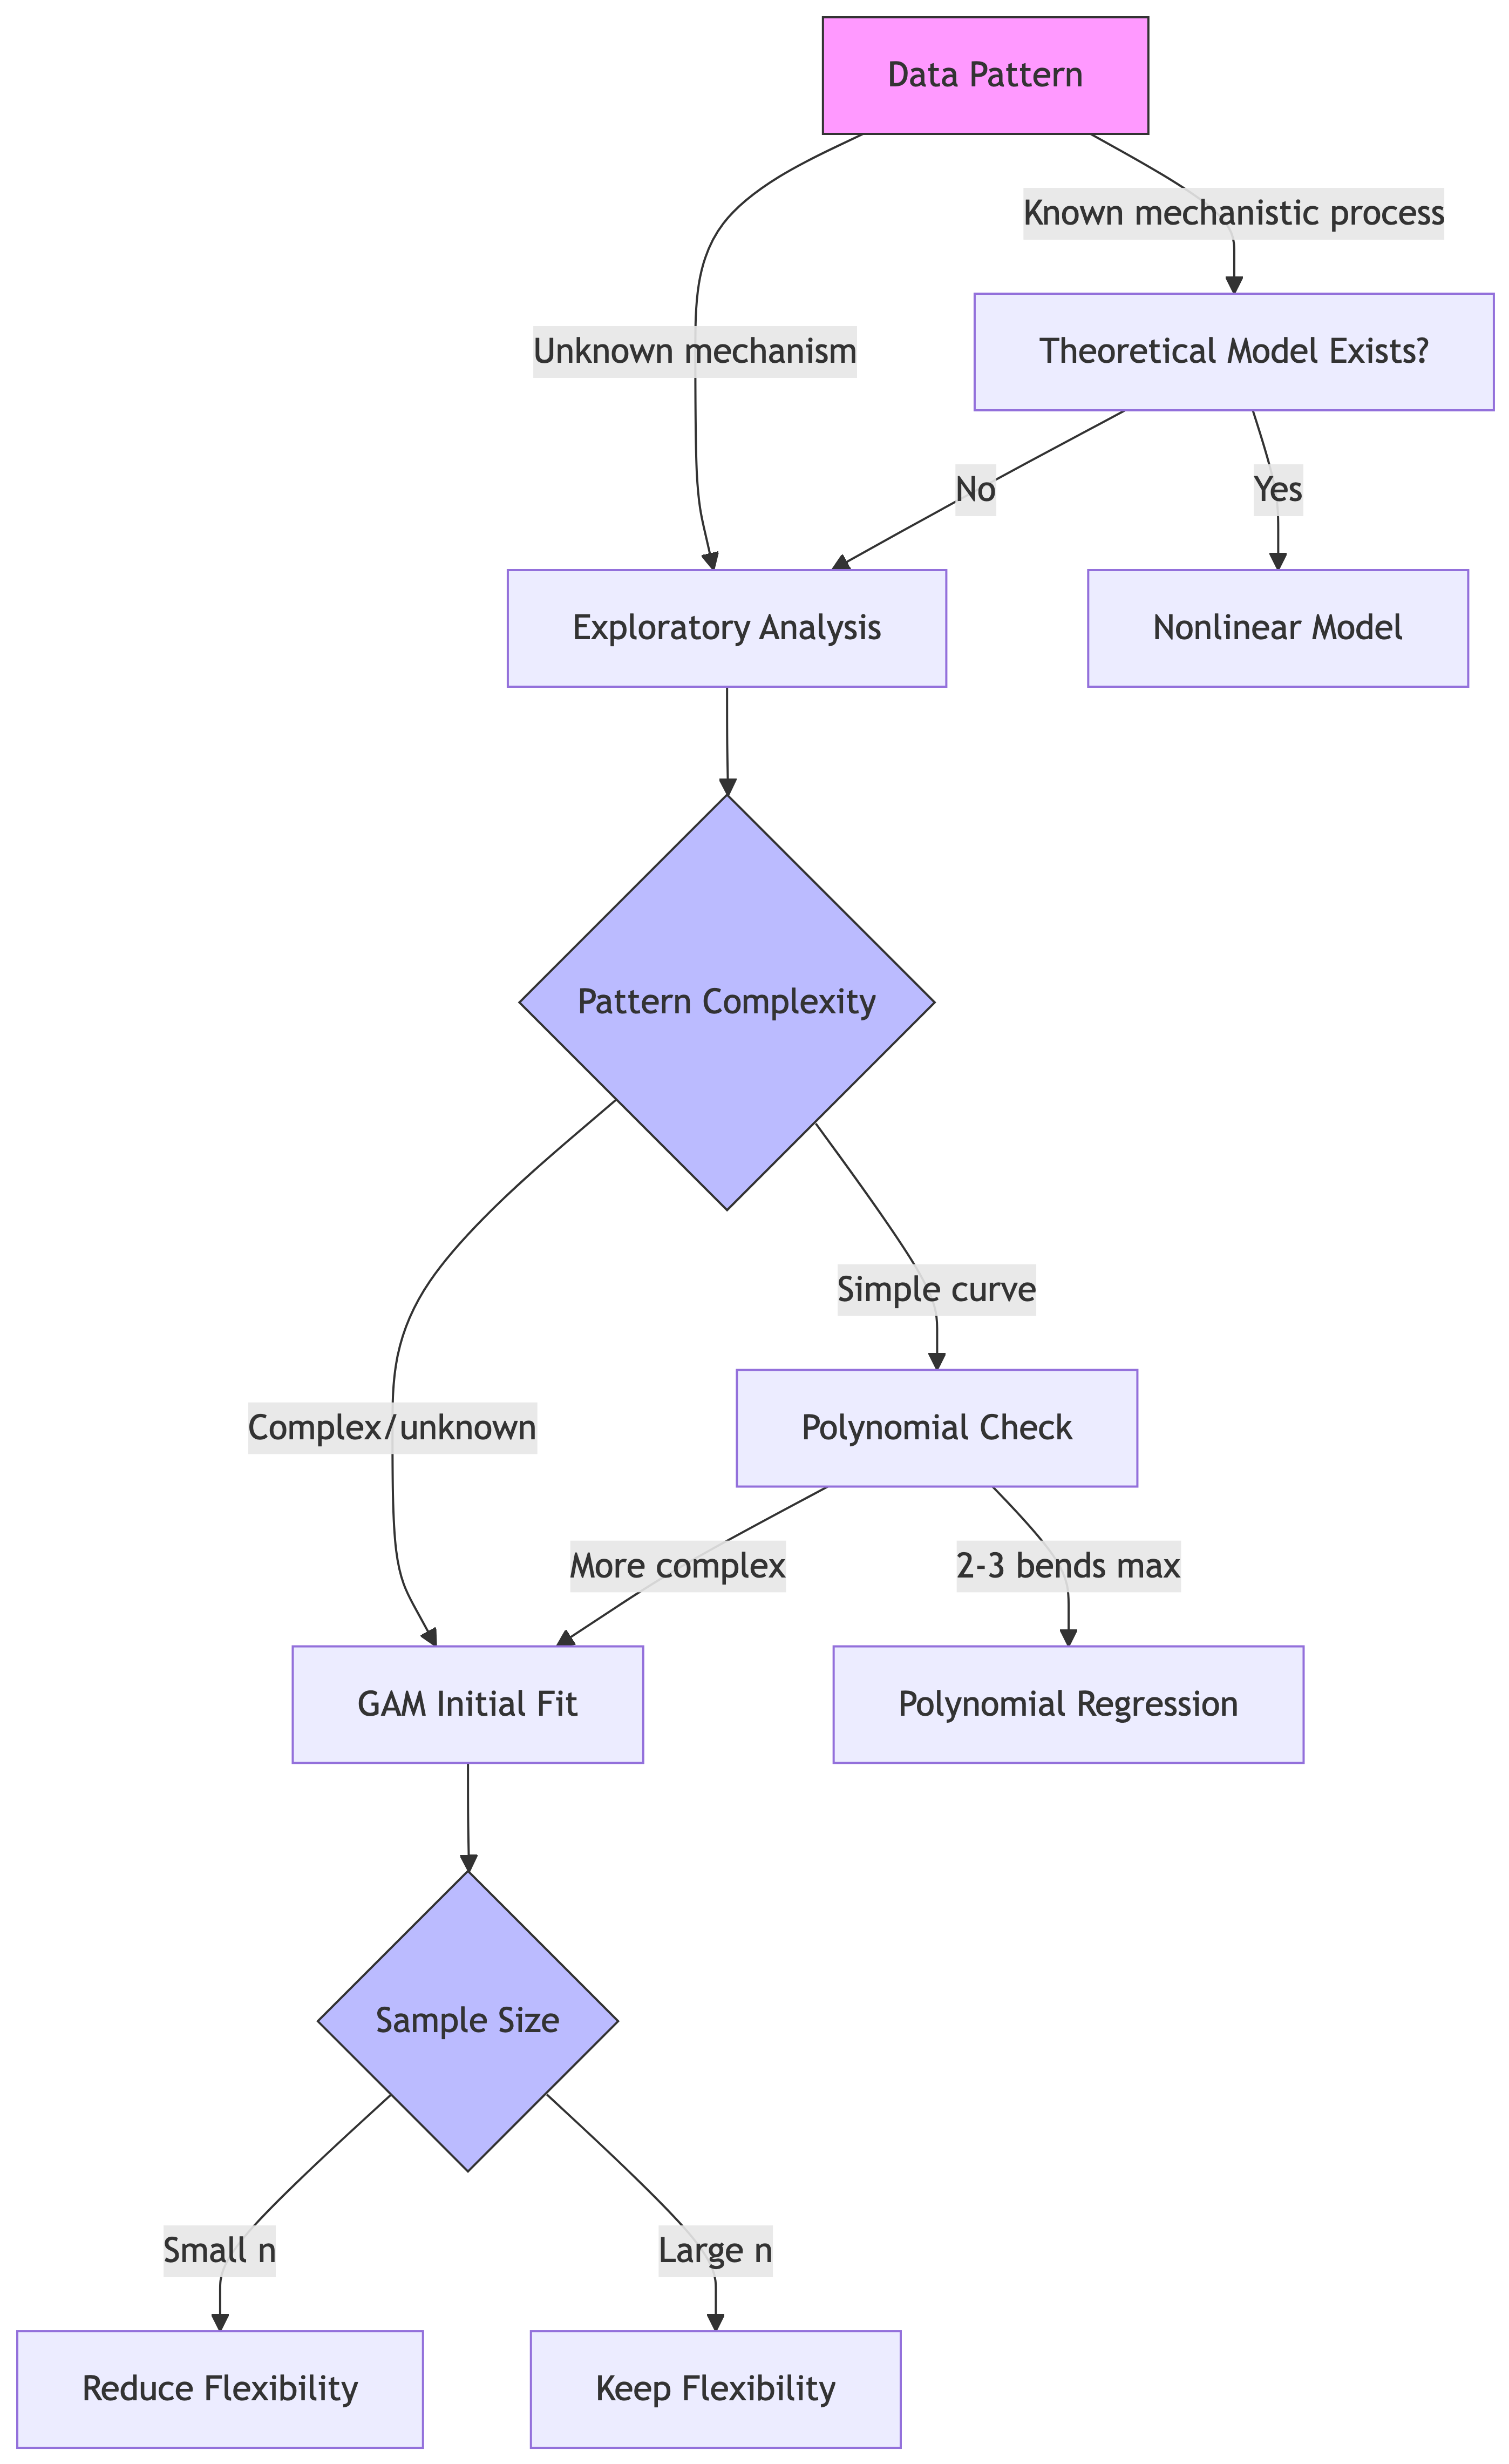
\includegraphics[width=3in,height=4.89in]{non-linear_regression_files/figure-latex/mermaid-figure-1.png}

\subsection{Linearity
vs.~Nonlinearity}\label{linearity-vs.-nonlinearity}

The first fork in our decision making process involves seeing if the
relationship between the variables is linear or can be adequately
approximated by a polynomial function, polynomial regression is a
suitable choice. Nonlinear models or GAMs may be more appropriate if the
relationship is nonlinear and does not follow a specific polynomial
form. In Figure~\ref{fig-combo}, it is obvious that the straight line
model is not a good fit for the data, but the second- and third-order
polynomial models, the GAM, and the von Bertalanffy model all provide
better fits.

\subsection{Complexity of the
Relationship}\label{complexity-of-the-relationship}

Polynomial regression is limited in its ability to capture complex
nonlinear relationships, especially those with more bends, peaks, or
valleys than a polynomial of order \textless3 (or even 4 at a push) can
capture. Another consideration is the process the data represent: if it
is inherently nonlinear according to a known function such as
exponential growth or decay, seasonal sinusoidal patterns, or logistic
growth, then nonlinear models or GAMs are more flexible and can capture
a wider range of nonlinear responses. In Figure~\ref{fig-combo}, the von
Bertalanffy model is a saturating growth model, which is a known
biological process that can be captured by a nonlinear model. The
3rd-order polynomial model also seems to capture a saturating growth
pattern, but it also somewhat influenced by the dip in the raw data
around 12.5 years (in addition to some other nuances), but this is
likely due to some random variation and is not part of the growth
response.

\subsection{Interpretability
vs.~Flexibility}\label{interpretability-vs.-flexibility}

Polynomial regression provides coefficients that relate to the powers of
the predictor variables, but the interpretation of the \(\beta\)
parameters is not as intuitive as in a linear model of order 1. In
contrast, nonlinear models and GAMs offer greater flexibility in
capturing complex patterns. GAMs may lack direct interpretability of the
coefficients, but the nonlinear model offers coefficients that can be
interpreted in the context of the model's structure. In
Figure~\ref{fig-combo}, the von Bertalanffy model has a clear biological
interpretation (see Section~\ref{sec-vonbertalanffy}), while the
3rd-order polynomial model and the GAM are more flexible and can capture
a wider range of shapes (it follows the dips and peaks in the raw data
closer). The 2nd-order polynomial does not fit the data as well at very
low ages at 20 year, but it is still a better fit than the linear model.

\subsection{Overfitting Concerns}\label{overfitting-concerns}

Polynomial regression with high-degree polynomials can lead to
overfitting, especially when the model complexity exceeds the underlying
data patterns. Nonlinear models and GAMs can also overfit if not
properly regularised or constrained. These insights can be seen when we
examine the summaries of the regression fits, and can be formally
assessed using cross-validation or information criteria. In
Figure~\ref{fig-combo}, the 3rd-order polynomial model seems to capture
some of the random variation in the data, which may be an indication of
overfitting. The GAM also seems to capture some of the random variation,
but it is less pronounced than in the 3rd-order polynomial model.

\subsection{Data Size and Complexity}\label{data-size-and-complexity}

For small to moderate-sized datasets with complex nonlinear
relationships, GAMs may be more suitable due to their flexibility and
ability to capture intricate patterns. For simpler relationships or when
interpretability is important, nonlinear regression (with
mechanistically-informed parameters) may be preferred. These are not of
concern in Figure~\ref{fig-combo}.

\subsection{Model Complexity and
Assumptions}\label{model-complexity-and-assumptions}

Polynomial regression assumes a specific polynomial form for the
relationship, which may not hold in practice. Nonlinear models and GAMs
are more flexible and do not always impose strict parametric assumptions
(see Section~\ref{sec-assumptions}), making them more robust to
deviations from the assumed form. A detailed assessment of the model
assumptions and the complexity of the relationship can help guide the
choice of model. We need to add to this our biologist specialist
knowledge to make the best choice.

\subsection{Computational
Considerations}\label{computational-considerations}

Polynomial regression is relatively simple to implement and
computationally efficient, especially for low-degree polynomials.
Nonlinear models and GAMs may require more computational resources,
especially for large datasets or complex models. Not a concern for the
models represented in Figure~\ref{fig-combo}.

\section{Requirements and Assumptions}\label{sec-assumptions}

Polynomial regression, nonlinear regression, and GAMs are built upon the
principles of linear regression; therefore, the fundamental assumptions
of normality and homoscedasticity of residuals usually still apply.
Specifically, these models assume that the residuals are independent and
identically distributed (i.i.d.), which implies that they are normally
distributed with a constant variance (homoscedasticity). However, the
specifics can vary depending on the model and the distribution of the
response variable. Of course, there is also the requirement for the
response variable to be continuous and independent. These assumptions
help ensure that the error terms (residuals) in the model are
well-behaved so that reliable inference and predictions can be obtained.

Nuances:

\begin{itemize}
\tightlist
\item
  \textbf{Polynomial Regression:} While a type of nonlinear regression,
  polynomial models are still linear in their parameters. This means
  that they are more bound to the classic regression assumptions and can
  be more sensitive to violations.
\item
  \textbf{GAMs:} Offer more flexibility in handling nonlinear
  relationships. Depending on the distributions used for the outcome
  variable and the link functions employed, GAMs can potentially relax
  some of the strict normality assumptions.
\item
  \textbf{Nonlinear Models in General:} Some truly nonlinear models
  (like those based on exponential or logarithmic functions) may have
  inherently different error structures and may not strictly require the
  same assumptions of normality and homoscedasticity. However, these
  models come with their own set of assumptions and considerations.
\end{itemize}

Important considerations:

\begin{itemize}
\tightlist
\item
  \textbf{Diagnostic Checks:} Regardless of the model type, it's
  \emph{essential} to perform residual diagnostics to assess if
  assumptions are met. Visualisations (e.g., histograms, Q-Q plots,
  residuals vs. fitted plots) are well-known tools.
\item
  \textbf{Transformations:} If violations of assumptions are found, data
  transformation techniques (e.g., Box-Cox, log) could be considered to
  improve model validity.
\item
  \textbf{Generalised Linear Models (GLMs):} An important class of
  models designed to handle various non-normal responses (e.g., count,
  binary) while extending the linear modeling framework. GLMs are good
  alternative to both polynomial regression and GAMs in certain
  contexts.
\item
  \textbf{Mixed models:} Linear Mixed Models (LLMs), Generalised Linear
  Mixed Models (GLMMs), and Generalised Nonlinear Models (GNLMs) can be
  used to account for dependencies in the data, such as repeated
  measures or hierarchical structures. GAMs also accommodate mixed data
  structures.
\end{itemize}

The rest of this chapter will focus on the practical aspects of fitting
polynomial regression models and nonlinear regressions in R. GAMs will
be covered in a separate chapter due to their unique characteristics and
implementation details.

\section{R Functions and Packages}\label{r-functions-and-packages}

\subsection{Polynomial Regression}\label{polynomial-regression-1}

To fit a polynomial model in R, use the simple linear regression
function \texttt{lm()} to fit the model. The purpose of \texttt{poly()}
is to generate polynomial terms of a specified degree. The basic form
is:

\begin{Shaded}
\begin{Highlighting}[]
\NormalTok{poly\_model }\OtherTok{\textless{}{-}} \FunctionTok{lm}\NormalTok{(y }\SpecialCharTok{\textasciitilde{}} \FunctionTok{poly}\NormalTok{(x, }\AttributeTok{degree =} \DecValTok{2}\NormalTok{), }\AttributeTok{data =}\NormalTok{ data)}
\end{Highlighting}
\end{Shaded}

GLMs are a generalisation of ordinary linear regression that allows for
the response variable to have non-Gaussian error distributions such as
one of the exponential family distributions (e.g., binomial, Poisson,
gamma). These distributions are accommodated via so-called link
functions within the GLM framework. The most common R function for
fitting GLMs is \texttt{glm()}.

Mixed models that include random and fixed effects (see box `Fixed and
Random Effects') are also available. These are necessary for the
analysis of data that have correlations within groups or hierarchies
(e.g., repeated measures\footnote{Repeated measures are multiple
  observations taken on the same subject or unit over time or under
  different conditions. Sometimes this is called longitudinal data.} or
the inclusion of grouped variables). Commonly used are \texttt{lmer()}
for LLMs and \texttt{glmer()} for GLMMs. Both functions are in the
\textbf{lme4} package. Another package that accommodates LLMs is
\textbf{nlme} and its \texttt{lme()} function. It has somewhat different
capabilities and syntax compared to \textbf{lme4}.

\begin{tcolorbox}[enhanced jigsaw, opacitybacktitle=0.6, toptitle=1mm, colframe=quarto-callout-note-color-frame, arc=.35mm, left=2mm, rightrule=.15mm, coltitle=black, opacityback=0, bottomrule=.15mm, bottomtitle=1mm, title=\textcolor{quarto-callout-note-color}{\faInfo}\hspace{0.5em}{Fixed and Random Effects}, toprule=.15mm, colbacktitle=quarto-callout-note-color!10!white, titlerule=0mm, leftrule=.75mm, colback=white, breakable]

Random effects and fixed effects are used in regression models to
account for different sources of variation in the data.

\emph{Fixed effects} are variables or factors that represent sources of
variation that are of primary interest in the study or that have a
finite and fixed number of levels or categories. These effects are
assumed to have an influence on the mean response. Examples of fixed
effects include:

\begin{itemize}
\tightlist
\item
  Treatment groups in an experiment (e.g., fertiliser A, fertiliser B,
  control)
\item
  Categorical variables (e.g., sex, age group, species)
\item
  Continuous variables (e.g., time, temperature, concentration)
\end{itemize}

The coefficients associated with fixed effects are estimated and
interpreted as the primary effects of interest in the model.

\emph{Random effects} are variables or factors that represent sources of
variation that are not of primary interest but need to be accounted for
in the model. These effects are assumed to be randomly sampled from a
larger population, and their levels are theoretically infinite or too
numerous to be modeled as fixed effects. Examples of random effects
include:

\begin{itemize}
\tightlist
\item
  Subjects or individuals in a study (e.g., individual plants or
  animals)
\item
  Clusters or groups (e.g., plots, aquaria, transects)
\item
  Repeated measures or time points within subjects
\end{itemize}

Random effects are used to model the correlation or dependence among
observations within the same cluster, subject, or time series. They
allow for subject-specific or cluster-specific adjustments to the
overall model, accounting for the fact that observations within the same
group are more similar than observations from different groups.

In LMMs and GLMMs, both fixed and random effects are included. The fixed
effects represent the primary effects of interest and the random effects
account for the correlation or dependence within clusters or subjects.

\end{tcolorbox}

\subsection{Nonlinear Regression}\label{nonlinear-regression}

In R, nonlinear regressions can be performed using the \texttt{nls()}
function in the \textbf{base} package. It uses iterative algorithms to
minimise the residual sum of squares and find the best-fit parameters
for the user-specified nonlinear model.

The \texttt{nls()} function is most frequently used to fit
user-specified nonlinear functions. The basic syntax is:

\begin{Shaded}
\begin{Highlighting}[]
\NormalTok{nls\_model }\OtherTok{\textless{}{-}} \FunctionTok{nls}\NormalTok{(y }\SpecialCharTok{\textasciitilde{}} \FunctionTok{f}\NormalTok{(x, theta1, theta2, ...), }\AttributeTok{data =}\NormalTok{ data,}
                 \AttributeTok{start =} \FunctionTok{list}\NormalTok{(}\AttributeTok{theta1 =}\NormalTok{ value1, }\AttributeTok{theta2 =}\NormalTok{ value2, ...))}
\end{Highlighting}
\end{Shaded}

GNLMs extend nonlinear models by allowing the response variable to
follow one of the exponential family distributions, such as binomial,
Poisson, or gamma, etc. This is done through a link function that
relates the mean of the distribution to the predictors through the
nonlinear model. GNLMs are fit using maximum likelihood estimation,
which is flexible enough to handle various types of error distribution
and link functions. The \textbf{gnm} package rovides the \texttt{gnm()}
function designed for this purpose.

For data with dependencies within groups or hierarchies (such as in
longitudinal studies), NLMMs are available within \texttt{nlme()}. NLMMs
incorporate fixed effects (associated with the nonlinear terms) and
random effects (to account for correlation and variation within groups).

\section{Example: Algal Nutrient Uptake Kinetcis}\label{sec-ex1}

We can measure algal nutrient uptake rates using two types of
experiments: multiple flask experiments and perturbation experiments.
The fundamental concept underlying both methods is to introduce a known
quantity of nutrients (termed the substrate) into a flask or a series of
flasks and then measure the rate of nutrient uptake (\(V\)) at different
substrate concentrations (\([S]\)). We calculate the nutrient uptake
rate as the change in nutrient concentration in the flask over a
predefined time interval (\(V = \Delta [S]/\Delta t\)). Consequently,
both experiments generate data that relate the nutrient uptake rate to
the corresponding substrate concentration. The primary difference
between the two methods lies in the experimental setup and the data
analysis.

In the \textbf{multiple flask method}, we prepare a series of flasks,
each containing a different initial concentration of the substrate
nutrient to span the range typically encountered by the specimen in its
natural environment. We then measure the nutrient uptake rate in
\emph{each individual flask} over a specific time period, for example by
taking measurements at the start (\(t=0\)) and end (\(t=30\) minutes) of
the incubation. We calculate the change in substrate concentration over
this time interval in each flask to determine the corresponding nutrient
uptake rate. The resulting data from this method therefore consists of
the different initial substrate concentrations used in each flask,
paired with their respective measured nutrient uptake rates over the
incubation period.

The \textbf{perturbation method} uses a single flask to which we add a
high initial concentration of the substrate nutrient, set at a level
that is ecologically meaningful and relevant to the study system.
Instead of using multiple flasks, we measure the change in the remaining
substrate concentration at multiple time points within this \emph{same
flask}, for example by taking samples every 10 or 20 minutes until all
the substrate is depleted, say at 120 minutes. We calculate the change
in substrate concentration between each successive time point to
determine the corresponding nutrient uptake rate over that time
interval. The resulting data, therefore, consist of a time series of
substrate concentrations at each measurement time point, paired with the
nutrient uptake rates calculated over the periods between those time
points.

The important differences between the multiple flask and perturbation
experiments are summarised in Table~\ref{tbl-diffs}.

\begin{longtable}[]{@{}
  >{\raggedright\arraybackslash}p{(\linewidth - 4\tabcolsep) * \real{0.1786}}
  >{\raggedright\arraybackslash}p{(\linewidth - 4\tabcolsep) * \real{0.3929}}
  >{\raggedright\arraybackslash}p{(\linewidth - 4\tabcolsep) * \real{0.4286}}@{}}
\caption{Key differences between multiple flask and perturbation
experiments.}\label{tbl-diffs}\tabularnewline
\toprule\noalign{}
\begin{minipage}[b]{\linewidth}\raggedright
Feature
\end{minipage} & \begin{minipage}[b]{\linewidth}\raggedright
Multiple Flask Experiments
\end{minipage} & \begin{minipage}[b]{\linewidth}\raggedright
Perturbation Experiments
\end{minipage} \\
\midrule\noalign{}
\endfirsthead
\toprule\noalign{}
\begin{minipage}[b]{\linewidth}\raggedright
Feature
\end{minipage} & \begin{minipage}[b]{\linewidth}\raggedright
Multiple Flask Experiments
\end{minipage} & \begin{minipage}[b]{\linewidth}\raggedright
Perturbation Experiments
\end{minipage} \\
\midrule\noalign{}
\endhead
\bottomrule\noalign{}
\endlastfoot
Experimental Setup & Multiple flasks, each with different \([S]\) &
Single flask with initial high \([S]\) \\
Data Independence & Data points are independent & Data points are
correlated (repeated measures) \\
Analysis & Nonlinear least squares regression (NLS) & Nonlinear mixed
model (NLMM) \\
R Function & \texttt{nls()} & \texttt{nlme::nlme()} \\
\end{longtable}

Our choice between multiple flask and perturbation experiments depends
on our research questions and experimental constraints. In both methods,
we must consider all sources of error and variability, such as
measurement error, the type of nutrient, the physiological state of the
alga, the light intensity, the experimental temperature, and other
variables that might affect the uptake response.

We apply the Michaelis-Menten model (Equation~\ref{eq-mm}) to data from
multiple flask and perturbation experiments to characterise nutrient
uptake. Applied to algae, this model assumes an irreversible uptake
process that saturates at high substrate concentrations. It effectively
quantifies key characteristics of the nutrient uptake system, including
the maximum uptake rate and the algae's affinity for the nutrient.

We use the \texttt{nls()} function to fit the Michaelis-Menten model to
the data from multiple flask experiments. For the perturbation
experiment, things are a bit more complicated. This method includes
dependent data points because the measurements are taken from the same
flask at different times, introducing a correlation between
observations. This violates the independence assumption required for
standard regression models. To accurately analyse these data, I
recommend a \emph{nonlinear mixed-effects model} implemented in the
\texttt{nlme()} function. Mixed-effects models account for fixed effects
(overall trends across all observations) and random effects (variations
specific to individual experimental units, in this case, time points
within the same flask). This helps handle the correlation between
repeated measures and produces reliable estimates of the uptake dynamics
within the flask.

The Michaelis-Menten equation is given by:

\begin{equation}\phantomsection\label{eq-mm}{V_i = \frac{V_{max} \cdot [S_i]}{K_m + [S_i]} + \epsilon_i}\end{equation}

Where:

\begin{itemize}
\tightlist
\item
  \(V_i\) is the uptake rate at the \(i\)-th observation,
\item
  \(V_{max}\) is the maximum nutrient uptake rate achieved,
\item
  \([S_i]\) is the substrate concentration at the \(i\)-th observation,
\item
  \(K_m\) is the Michaelis constant, which represents the substrate
  concentration at which the uptake rate is half of \(V_{max}\), and
\item
  \(\epsilon_i\) is the error term at the \(i\)-th observation. and
\end{itemize}

The two parameters of the Michaelis-Menten model are rooted in theory
and have ecophysiological interpretations. \(K_m\) is a measure of the
alga's affinity for the nutrient and is determined by the kinetic
constants governing the formation and dissociation of the
enzyme-substrate complex responsible for taking up the nutrient; lower
values indicate a higher affinity. \(V_{max}\) represents the maximum
capacity of the alga to utilise the nutrient.

\subsection{Hypothesis Testing and the Michaelis-Menten
Model}\label{hypothesis-testing-and-the-michaelis-menten-model}

\subsubsection{Linear vs.~Michaelis-Menten
Model}\label{sec-linear-vs-mm}

Often, we aim to understand the relationship between two variables but
we may not yet know which model best describes this relationship. For
instance, in algal nutrient uptake kinetics, both a linear model and a
nonlinear Michaelis-Menten model can be used to describe the
relationship between nutrient uptake rate and substrate concentration.
Both models are valid but they have different interpretations and unique
ecophysiological implications. The choice between the two models depends
on the biological system.

\begin{itemize}
\tightlist
\item
  \textbf{Linear models} indicate that the uptake process is inherently
  unsaturated, such as with the uptake of ammonium. In this case, the
  uptake rate continues to increase linearly with substrate
  concentration.
\item
  The \textbf{Michaelis-Menten model} suggests that the uptake rate
  eventually saturates as the substrate concentration increases, which
  is often the case with nitrate.
\end{itemize}

The key question is: How do we decide which model fits our data best?

The simplest way is to visually inspect the scatter of points on a plot
of the \(V\) vs.~\([S]\) data, which would be part of any exploratory
data analysis. If the data exhibit a clear saturation pattern, where the
uptake rate levels off at high substrate concentrations, the
Michaelis-Menten model is likely to provide a better fit. Conversely, if
the data show a linear relationship over the observed range of substrate
concentrations, the linear model may be more appropriate.

It is also important to consider the biological plausibility of the
models. If there is prior knowledge or theoretical reasons to expect a
saturating relationship between the uptake rate and substrate
concentration, the Michaelis-Menten model may be more appropriate, even
if both models provide a similar fit to the data.

Confirmation can be obtained by fitting both models to our data and
comparing their performance using statistical measures such as the sum
of squared residuals (SSR), Akaike Information Criterion (AIC), Bayesian
Information Criterion (BIC), or log-likelihood test.

To proceed with the statistical approach, we must first set hypotheses
such as these to compare the models:

\textbf{\(H_0\):} The Michaelis-Menten model does not provide a better
fit to the data than a simple linear model.

In other words, we suggest with the null hypothesis that the
relationship between nutrient uptake rate and the substrate
concentration is adequately described by a linear model rather than the
Michaelis-Menten nonlinear model. The implication is that the uptake
rate increases linearly with substrate concentration, without
saturation.

\textbf{\(H_a\):} The Michaelis-Menten model provides a significantly
better fit to the data than a simple linear model.

With the alternative hypothesis we propose that the relationship between
the nutrient uptake rate and the substrate concentration is best
described by the nonlinear Michaelis-Menten model, so the uptake rate
initially increases with substrate concentration but eventually levels
off, indicating saturation.

To test these hypotheses, we can:

\begin{enumerate}
\def\labelenumi{\arabic{enumi}.}
\tightlist
\item
  Fit both the Michaelis-Menten model and a linear model to the data.
\item
  Compare the goodness-of-fit of both models using statistical measures
  such as the SSR, AIC, or BIC.
\item
  Perform a model comparison test (such as an \emph{F}-test or
  likelihood ratio test) to determine if the improvement in fit provided
  by the Michaelis-Menten model is statistically significant compared to
  the linear model.
\end{enumerate}

In the above scenario, which is to decide among the linear and
Michaelis-Menten models, hypotheses concerning the parameters of the
models are not directly tested as they are not really of interest
(except for estimating their magnitude, perhaps). Instead, the focus is
on the overall goodness-of-fit of the models to the data.

\subsubsection{Comparing Two Michaelis-Menten
Models}\label{sec-mm-comparison}

Here, we may be interested in testing whether the parameters
\(V_\text{max}\) and \(K_m\) differ from some hypothesised values or
across different experimental conditions.

In the first instance, we can set up the hypotheses as follows:

\textbf{\(H_0:\)} \(V_\text{max} = V_\text{max}^*\) and \(K_m = K_m^*\)

where \(V_\text{max}^*\) and \(K_m^*\) are the hypothesised values (or
values from a reference condition) for the maximum uptake rate and
Michaelis constant, respectively.

\textbf{\(H_a:\)} \(V_\text{max} \neq V_\text{max}^*\) or
\(K_m \neq K_m^*\)

This alternative hypothesis states that at least one of the parameters
(\(V_\text{max}\) or \(K_m\)) differs from the hypothesised value.

If the experiment involves different experimental conditions or
treatments, we can modify the hypotheses accordingly. For example, if we
want to test whether the parameters differ between two experimental
conditions (A and B), the hypotheses could be:

\(H_0: V_\text{max}^A = V_\text{max}^B\) and \(K_m^A = K_m^B\)

\(H_a: V_\text{max}^A \neq V_\text{max}^B\) or \(K_m^A \neq K_m^B\)

In this case, the null hypothesis states that the maximum uptake rate
and Michaelis constant are the same for both experimental conditions,
while the alternative hypothesis states that at least one of the
parameters differs between the two conditions.

After fitting the Michaelis-Menten model to the data using the
\texttt{nls()} or \texttt{nlme()} functions in R, appropriate
statistical tests (e.g., likelihood ratio tests, Wald tests, or other
model comparison techniques) can be performed to evaluate the hypotheses
and determine whether the parameter estimates significantly differ from
the hypothesised values or across experimental conditions.

\subsection{Multiple Flask Experiment}\label{multiple-flask-experiment}

\subsubsection{Fitting a single model (NLS)}\label{sec-mf-single}

To demonstrate fitting a nonlinear model to \(V\) vs \([S]\) data
produced from a multiple flask experiment, I simulate data across a
range of substrate concentrations. We then fit the model to the data
using the \texttt{nls()} function in R. The dataset consists of five
replicate flask sets (\(n=5\)) for each of 13 substrate concentrations.
Each set therefore results in independently estimated uptake rates for
the initial nutrient concentrations. The dataset is shown in
Table~\ref{tbl-mf1}, and a plot of \(V\) as a function of \([S]\) is
shown in Figure~\ref{fig-mf1}.

\begin{table}

\caption{\label{tbl-mf1}Simulated data for a multiple flask experiment
on an alga (showing only the top and bottom three rows).}

\centering{

\fontsize{12.0pt}{14.4pt}\selectfont
\begin{tabular*}{\linewidth}{@{\extracolsep{\fill}}crr}
\toprule
Replicate flask & [S] & V \\ 
\midrule\addlinespace[2.5pt]
1 & 0 & 0.00 \\ 
2 & 0 & 0.00 \\ 
3 & 0 & 0.00 \\ 
3 & 30 & 37.64 \\ 
4 & 30 & 37.97 \\ 
5 & 30 & 35.95 \\ 
\bottomrule
\end{tabular*}

}

\end{table}%

\begin{figure}[t]

\centering{

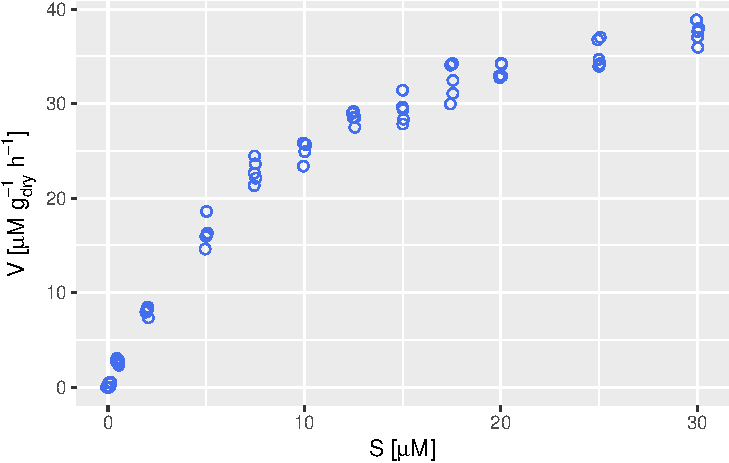
\includegraphics[width=0.8\linewidth,height=\textheight,keepaspectratio]{index_files/mediabag/non-linear_regression_files/figure-pdf/fig-mf1-1.pdf}

}

\caption{\label{fig-mf1}Plot of \(V\) as a function of \([S]\) for a
multiple flask experiment involving seven replicate flask sets.}

\end{figure}%

In Figure~\ref{fig-mf1}, there is a clear indication that the uptake
rates plateau at higher substrate concentrations, suggesting that
fitting a Michaelis-Menten model is advisable. Later, I will compare
this with a linear model for completeness. A central feature of this
dataset is that the data were collected independently, with each flask
set representing a separate experimental unit. There is no correlation
between flasks within a set, and no correlation across the initial
substrate concentrations. Consequently, the assumption of independence
is fully met, allowing the simplest expression of the \texttt{nls()}
function to be used to fit the Michaelis-Menten model to the data.

The Michaelis-Menten model is fit to the data using the \texttt{nls()}
function in R. It is specified as:

\phantomsection\label{annotated-cell-56}%
\begin{Shaded}
\begin{Highlighting}[]
\CommentTok{\# Define the model function}
\NormalTok{mm\_fun }\OtherTok{\textless{}{-}} \ControlFlowTok{function}\NormalTok{(S, Vmax, Km) \{}
\NormalTok{  Vmax }\SpecialCharTok{*}\NormalTok{ S }\SpecialCharTok{/}\NormalTok{ (Km }\SpecialCharTok{+}\NormalTok{ S)}
\NormalTok{\}}

\CommentTok{\# Fit the nonlinear model Michaelis{-}Menten model}
\NormalTok{nls\_mod }\OtherTok{\textless{}{-}} \FunctionTok{nls}\NormalTok{(V }\SpecialCharTok{\textasciitilde{}} \FunctionTok{mm\_fun}\NormalTok{(S, Vmax, Km), }\hspace*{\fill}\NormalTok{\circled{1}}
            \AttributeTok{data =}\NormalTok{ mf\_data,}
            \AttributeTok{start =} \FunctionTok{c}\NormalTok{(}\AttributeTok{Vmax =} \DecValTok{30}\NormalTok{, }\AttributeTok{Km =} \DecValTok{5}\NormalTok{)) }\hspace*{\fill}\NormalTok{\circled{2}}
\end{Highlighting}
\end{Shaded}

\begin{description}
\tightlist
\item[\circled{1}]
The model formula specifies the Michaelis-Menten equation, with
\texttt{V} as the dependent variable on the left-hand side and
\texttt{S} as the independent variable on the right. The model
parameters \texttt{Vmax} and \texttt{Km} will be estimated when fitting
the model.
\item[\circled{2}]
The \texttt{start} argument provides initial values for the model
parameters. The \texttt{Vmax} and \texttt{Km} parameters are estimated
by minimising the sum of squared residuals between the observed and
predicted values of \texttt{V}. The \texttt{nls()} function uses an
iterative process to find the best-fitting values for these parameters,
and the starting values improve the success of model convergence.
\end{description}

Here is the model summary:

\begin{Shaded}
\begin{Highlighting}[]
\FunctionTok{summary}\NormalTok{(nls\_mod)}
\SpecialCharTok{\textgreater{}} 
\ErrorTok{\textgreater{}}\NormalTok{ Formula}\SpecialCharTok{:}\NormalTok{ V }\SpecialCharTok{\textasciitilde{}} \FunctionTok{mm\_fun}\NormalTok{(S, Vmax, Km)}
\SpecialCharTok{\textgreater{}} 
\ErrorTok{\textgreater{}}\NormalTok{ Parameters}\SpecialCharTok{:}
\ErrorTok{\textgreater{}}\NormalTok{      Estimate Std. Error t value }\FunctionTok{Pr}\NormalTok{(}\SpecialCharTok{\textgreater{}}\ErrorTok{|}\NormalTok{t}\SpecialCharTok{|}\NormalTok{)    }
\SpecialCharTok{\textgreater{}}\NormalTok{ Vmax  }\FloatTok{49.2444}     \FloatTok{0.8924}   \FloatTok{55.18}   \SpecialCharTok{\textless{}}\FloatTok{2e{-}16} \SpecialCharTok{**}\ErrorTok{*}
\ErrorTok{\textgreater{}}\NormalTok{ Km     }\FloatTok{9.4953}     \FloatTok{0.4474}   \FloatTok{21.22}   \SpecialCharTok{\textless{}}\FloatTok{2e{-}16} \SpecialCharTok{**}\ErrorTok{*}
\ErrorTok{\textgreater{}} \SpecialCharTok{{-}{-}{-}}
\ErrorTok{\textgreater{}}\NormalTok{ Signif. codes}\SpecialCharTok{:}  \DecValTok{0} \StringTok{\textquotesingle{}***\textquotesingle{}} \FloatTok{0.001} \StringTok{\textquotesingle{}**\textquotesingle{}} \FloatTok{0.01} \StringTok{\textquotesingle{}*\textquotesingle{}} \FloatTok{0.05} \StringTok{\textquotesingle{}.\textquotesingle{}} \FloatTok{0.1} \StringTok{\textquotesingle{} \textquotesingle{}} \DecValTok{1}
\SpecialCharTok{\textgreater{}} 
\ErrorTok{\textgreater{}}\NormalTok{ Residual standard error}\SpecialCharTok{:} \FloatTok{1.092}\NormalTok{ on }\DecValTok{63}\NormalTok{ degrees of freedom}
\SpecialCharTok{\textgreater{}} 
\ErrorTok{\textgreater{}}\NormalTok{ Number of iterations to convergence}\SpecialCharTok{:} \DecValTok{4} 
\SpecialCharTok{\textgreater{}}\NormalTok{ Achieved convergence tolerance}\SpecialCharTok{:} \FloatTok{4.705e{-}07}
\end{Highlighting}
\end{Shaded}

The above output provides the estimates for \(V_{\max}\) and \(K_m\),
along with their standard errors, \emph{t}-values, and \emph{p}-values:

\begin{itemize}
\tightlist
\item
  The estimated maximum uptake rate (\(V_{\max}\)) is approximately
  49.24 \(\mu M N g^{-1} hr^{-1}\) and the small standard error
  associated with this parameter (0.89) indicates a precise estimate.
  The \emph{t}-value (55.18) is very high, and the corresponding
  \emph{p}-value is extremely small (\textless0.0001), indicating that
  \(V_{\max}\) is highly significantly different from zero.
\item
  The estimated Michaelis constant (\(K_m\)) is approximately 9.50
  \(\mu M\) and its standard error (0.45) is also small, suggesting a
  precise estimate. The \emph{t}-value (21.22) and the very small
  \emph{p}-value (\textless0.0001) indicate that \(K_m\) is also highly
  significantly different from zero.
\item
  The residual standard error is 1.10 on 63 degrees of freedom,
  indicating the average deviation of the observed uptake rates from the
  fitted model values.
\item
  The model converged in 4 iterations with a very small convergence
  tolerance, indicating a good fit and stability of the model.
\end{itemize}

\begin{tcolorbox}[enhanced jigsaw, opacitybacktitle=0.6, toptitle=1mm, colframe=quarto-callout-tip-color-frame, arc=.35mm, left=2mm, rightrule=.15mm, coltitle=black, opacityback=0, bottomrule=.15mm, bottomtitle=1mm, title=\textcolor{quarto-callout-tip-color}{\faLightbulb}\hspace{0.5em}{Results}, toprule=.15mm, colbacktitle=quarto-callout-tip-color!10!white, titlerule=0mm, leftrule=.75mm, colback=white, breakable]

The Michaelis-Menten parameters, maximum uptake rate (\(V_{\max}\)) and
half-saturation constant (\(K_m\)), were estimated using nonlinear
regression (Figure~\ref{fig-mf2}). The estimated \(V_{\max}\) was 49.24
\(\mu\)M N g\(^{-1}\) hr\(^{-1}\) (SE = 0.89, \(t = 55.18\),
\(p < 0.0001\)), and the estimated \(K_m\) was 9.50 \(\mu\)M (SE = 0.45,
\(t = 21.22\), \(p < 0.0001\)). Both parameters were significantly
different from zero. The model fit was good, converging in 3 iterations
with a residual standard error of 1.10 (63 degrees of freedom).

\end{tcolorbox}

\begin{figure}[tbp]

\centering{

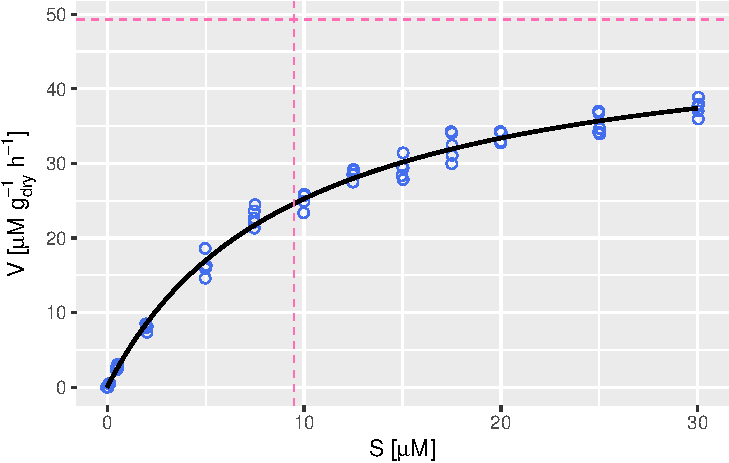
\includegraphics[width=0.8\linewidth,height=\textheight,keepaspectratio]{index_files/mediabag/non-linear_regression_files/figure-pdf/fig-mf2-1.pdf}

}

\caption{\label{fig-mf2}Plot of the Michaelis-Menten model fitted to the
data in Figure~\ref{fig-mf1}. The vertical and horizontal dashed lines
indicate the estimated \(K_m\) and \(V_{max}\) values, respectively.}

\end{figure}%

The text is clear and concise, but here are a few minor changes for
improved readability and precision:

\textbf{Assumption tests} Since these data are simulated and drawn from
a normal distribution with equal variances across the range of substrate
concentrations, the assumptions of homoscedasticity and normality of
residuals are inherently met. In this example, we fit the model solely
to obtain estimates of the Michaelis-Menten parameters, rather than to
make predictions, inferences, or calculate confidence intervals.
Therefore, assumption tests are not critical at this stage. We will
formally test assumptions in Section~\ref{sec-mf-treatments} when
comparing the effects of experimental treatments on kinetic parameters.

\subsubsection{Is the Michaelis-Menten model a better fit than a linear
model?}\label{is-the-michaelis-menten-model-a-better-fit-than-a-linear-model}

In Section~\ref{sec-linear-vs-mm}, we pose a hypothesis that requires
comparing a linear model to a Michaelis-Menten model fitted to the same
data. Figure~\ref{fig-mf2} indicates the nonlinear model indeed provides
a very good fit but in some situations this distinction may be less
clear and require verification. Let us fit a linear model to the above
data and compare it to the Michaelis-Menten model.

\begin{Shaded}
\begin{Highlighting}[]
\CommentTok{\# Fit the linear model}
\NormalTok{lm\_mod }\OtherTok{\textless{}{-}} \FunctionTok{lm}\NormalTok{(V }\SpecialCharTok{\textasciitilde{}}\NormalTok{ S, }\AttributeTok{data =}\NormalTok{ mf\_data)}

\FunctionTok{summary}\NormalTok{(lm\_mod)}
\SpecialCharTok{\textgreater{}} 
\ErrorTok{\textgreater{}}\NormalTok{ Call}\SpecialCharTok{:}
\ErrorTok{\textgreater{}} \FunctionTok{lm}\NormalTok{(}\AttributeTok{formula =}\NormalTok{ V }\SpecialCharTok{\textasciitilde{}}\NormalTok{ S, }\AttributeTok{data =}\NormalTok{ mf\_data)}
\SpecialCharTok{\textgreater{}} 
\ErrorTok{\textgreater{}}\NormalTok{ Residuals}\SpecialCharTok{:}
\ErrorTok{\textgreater{}}\NormalTok{    Min     }\DecValTok{1}\NormalTok{Q Median     }\DecValTok{3}\NormalTok{Q    Max }
\SpecialCharTok{\textgreater{}} \SpecialCharTok{{-}}\FloatTok{9.354} \SpecialCharTok{{-}}\FloatTok{4.791}  \FloatTok{0.580}  \FloatTok{4.948}  \FloatTok{8.293} 
\SpecialCharTok{\textgreater{}} 
\ErrorTok{\textgreater{}}\NormalTok{ Coefficients}\SpecialCharTok{:}
\ErrorTok{\textgreater{}}\NormalTok{             Estimate Std. Error t value }\FunctionTok{Pr}\NormalTok{(}\SpecialCharTok{\textgreater{}}\ErrorTok{|}\NormalTok{t}\SpecialCharTok{|}\NormalTok{)    }
\SpecialCharTok{\textgreater{}}\NormalTok{ (Intercept)  }\FloatTok{6.46005}    \FloatTok{0.98044}   \FloatTok{6.589} \FloatTok{1.03e{-}08} \SpecialCharTok{**}\ErrorTok{*}
\ErrorTok{\textgreater{}}\NormalTok{ S            }\FloatTok{1.29488}    \FloatTok{0.06683}  \FloatTok{19.376}  \SpecialCharTok{\textless{}} \FloatTok{2e{-}16} \SpecialCharTok{**}\ErrorTok{*}
\ErrorTok{\textgreater{}} \SpecialCharTok{{-}{-}{-}}
\ErrorTok{\textgreater{}}\NormalTok{ Signif. codes}\SpecialCharTok{:}  \DecValTok{0} \StringTok{\textquotesingle{}***\textquotesingle{}} \FloatTok{0.001} \StringTok{\textquotesingle{}**\textquotesingle{}} \FloatTok{0.01} \StringTok{\textquotesingle{}*\textquotesingle{}} \FloatTok{0.05} \StringTok{\textquotesingle{}.\textquotesingle{}} \FloatTok{0.1} \StringTok{\textquotesingle{} \textquotesingle{}} \DecValTok{1}
\SpecialCharTok{\textgreater{}} 
\ErrorTok{\textgreater{}}\NormalTok{ Residual standard error}\SpecialCharTok{:} \FloatTok{5.13}\NormalTok{ on }\DecValTok{63}\NormalTok{ degrees of freedom}
\SpecialCharTok{\textgreater{}}\NormalTok{ Multiple R}\SpecialCharTok{{-}}\NormalTok{squared}\SpecialCharTok{:}  \FloatTok{0.8563}\NormalTok{,  Adjusted R}\SpecialCharTok{{-}}\NormalTok{squared}\SpecialCharTok{:}  \FloatTok{0.854} 
\SpecialCharTok{\textgreater{}}\NormalTok{ F}\SpecialCharTok{{-}}\NormalTok{statistic}\SpecialCharTok{:} \FloatTok{375.4}\NormalTok{ on }\DecValTok{1}\NormalTok{ and }\DecValTok{63}\NormalTok{ DF,  p}\SpecialCharTok{{-}}\NormalTok{value}\SpecialCharTok{:} \ErrorTok{\textless{}} \FloatTok{2.2e{-}16}
\end{Highlighting}
\end{Shaded}

The linear model summary shows that the slope and intercept are
significantly different from zero, indicating a good fit. The \(R^2\)
value is 0.86, which is very high, suggesting that the linear model
explains 86\% of the variance in the data. The residual standard error
is 5.13, which is higher than the Michaelis-Menten model, indicating a
worse fit. We can test the difference between the models formally by
examining the AIC, BIC, or SSR, and the likelihood ratio test.

\begin{Shaded}
\begin{Highlighting}[]
\FunctionTok{AIC}\NormalTok{(lm\_mod, nls\_mod)}
\SpecialCharTok{\textgreater{}}\NormalTok{         df      AIC}
\SpecialCharTok{\textgreater{}}\NormalTok{ lm\_mod   }\DecValTok{3} \FloatTok{400.9933}
\SpecialCharTok{\textgreater{}}\NormalTok{ nls\_mod  }\DecValTok{3} \FloatTok{199.8814}
\end{Highlighting}
\end{Shaded}

\begin{Shaded}
\begin{Highlighting}[]
\FunctionTok{BIC}\NormalTok{(lm\_mod, nls\_mod)}
\SpecialCharTok{\textgreater{}}\NormalTok{         df      BIC}
\SpecialCharTok{\textgreater{}}\NormalTok{ lm\_mod   }\DecValTok{3} \FloatTok{407.5164}
\SpecialCharTok{\textgreater{}}\NormalTok{ nls\_mod  }\DecValTok{3} \FloatTok{206.4046}
\end{Highlighting}
\end{Shaded}

\begin{Shaded}
\begin{Highlighting}[]
\CommentTok{\# Calculate the sum of squared residuals (SSR)}
\FunctionTok{sum}\NormalTok{(}\FunctionTok{residuals}\NormalTok{(lm\_mod)}\SpecialCharTok{\^{}}\DecValTok{2}\NormalTok{)}
\SpecialCharTok{\textgreater{}}\NormalTok{ [}\DecValTok{1}\NormalTok{] }\FloatTok{1657.938}
\FunctionTok{sum}\NormalTok{(}\FunctionTok{residuals}\NormalTok{(nls\_mod)}\SpecialCharTok{\^{}}\DecValTok{2}\NormalTok{)}
\SpecialCharTok{\textgreater{}}\NormalTok{ [}\DecValTok{1}\NormalTok{] }\FloatTok{75.13611}
\end{Highlighting}
\end{Shaded}

\begin{Shaded}
\begin{Highlighting}[]
\FunctionTok{anova}\NormalTok{(lm\_mod, nls\_mod)}
\SpecialCharTok{\textgreater{}}\NormalTok{ Analysis of Variance Table}
\SpecialCharTok{\textgreater{}} 
\ErrorTok{\textgreater{}}\NormalTok{ Response}\SpecialCharTok{:}\NormalTok{ V}
\SpecialCharTok{\textgreater{}}\NormalTok{           Df Sum Sq Mean Sq F value    }\FunctionTok{Pr}\NormalTok{(}\SpecialCharTok{\textgreater{}}\NormalTok{F)    }
\SpecialCharTok{\textgreater{}}\NormalTok{ S          }\DecValTok{1} \FloatTok{9879.9}  \FloatTok{9879.9}  \FloatTok{375.43} \SpecialCharTok{\textless{}} \FloatTok{2.2e{-}16} \SpecialCharTok{**}\ErrorTok{*}
\ErrorTok{\textgreater{}}\NormalTok{ Residuals }\DecValTok{63} \FloatTok{1657.9}    \FloatTok{26.3}                      
\SpecialCharTok{\textgreater{}} \SpecialCharTok{{-}{-}{-}}
\ErrorTok{\textgreater{}}\NormalTok{ Signif. codes}\SpecialCharTok{:}  \DecValTok{0} \StringTok{\textquotesingle{}***\textquotesingle{}} \FloatTok{0.001} \StringTok{\textquotesingle{}**\textquotesingle{}} \FloatTok{0.01} \StringTok{\textquotesingle{}*\textquotesingle{}} \FloatTok{0.05} \StringTok{\textquotesingle{}.\textquotesingle{}} \FloatTok{0.1} \StringTok{\textquotesingle{} \textquotesingle{}} \DecValTok{1}
\end{Highlighting}
\end{Shaded}

The AIC, BIC, and SSR values for the Michaelis-Menten model are lower
than those for the linear model. Low is good, and we conclude that the
Michaelis-Menten model is a better fit. The likelihood ratio test also
shows that the Michaelis-Menten model is significantly better than the
linear model (d.f. = 1, \(F=375.43\), \(p<0.0001\)). Therefore, we can
conclude that the Michaelis-Menten model is the most appropriate model
for these data and that the rate of nutrient uptake by the seaweed (in
this example) is saturated at high nutrient concentrations.

\subsubsection{Comparing treatment effects (NLS and
NLMM)}\label{sec-mf-treatments}

Experiments are seldom as simple as the one above. To develop our
example further, consider an experiment designed to assess whether an
experimental treatment, such as light intensity or seawater temperature,
affects the nutrient uptake rate of a seaweed. It is biologically
plausible to expect that each treatment will result in unique
\(V_{max}\) and/or \(K_m\) values. For example, we know that the uptake
rate of nitrate (\ce{NO3-}) might increase at higher light intensities
and higher temperatures. Therefore, our hypothesis for this experiment
is that the nutrient uptake kinetics of the seaweed is influenced by the
treatment, as more formally stated in Section~\ref{sec-mm-comparison}.
To test this hypothesis, we fit a Michaelis-Menten model so that it
allows estimates of \(V_{max}\) and \(K_m\) to vary among treatment
groups.

The data for a multiple flask experiment with a treatment effect
comprised of three levels are provided in Table~\ref{tbl-mf2}. Except
for a new variable (treatment), the data are in all other respects
identical to those in Section~\ref{sec-mf-single}.

\begin{table}

\caption{\label{tbl-mf2}Simulated data with three treatment levels for a
multiple flask experiment on a seaweed species.}

\centering{

\fontsize{12.0pt}{14.4pt}\selectfont
\begin{tabular*}{\linewidth}{@{\extracolsep{\fill}}ccrr}
\toprule
Treatment & Replicate flask & [S] & V \\ 
\midrule\addlinespace[2.5pt]
Treatment 1 & 1 & 0 & 0.00 \\ 
Treatment 1 & 2 & 0 & 0.00 \\ 
Treatment 1 & 3 & 0 & 0.00 \\ 
Treatment 3 & 3 & 30 & 17.19 \\ 
Treatment 3 & 4 & 30 & 16.66 \\ 
Treatment 3 & 5 & 30 & 16.00 \\ 
\bottomrule
\end{tabular*}

}

\end{table}%

\textbf{Option 1} The \texttt{nls()} function in R does not handle
factor variables directly, which means we cannot include the treatment
variable as a factor in the model formula. To address this limitation,
we fit the \texttt{nls()} model separately for each treatment group.
This approach allows each treatment to have its own \(V_{\max}\) and
\(K_m\) values, effectively accommodating the variability in the
Michaelis-Menten parameters across treatments.

In addition to fitting separate models for each treatment, we also fit a
global model (a null model) to all the data. The global model assumes
that the effect of the experimental treatment is negligible, meaning
that all treatments share the same \(V_{\max}\) and \(K_m\). This global
fit serves as a baseline for comparison.

To determine whether the Michaelis-Menten parameters significantly
differ among the treatment groups, we perform a likelihood ratio test.
The likelihood ratio test compares the fit of the global model (where
parameters are shared across treatments) to the combined fit of the
separate models (where parameters vary by treatment). The test statistic
is the difference in the log-likelihoods of the two models, which
follows a \(\chi^2\) distribution with degrees of freedom equal to the
difference in the number of parameters between the two models.

\begin{Shaded}
\begin{Highlighting}[]
\CommentTok{\# Fit separate models}
\NormalTok{separate\_models }\OtherTok{\textless{}{-}}\NormalTok{ mf\_data2 }\SpecialCharTok{|\textgreater{}}
  \FunctionTok{group\_by}\NormalTok{(trt) }\SpecialCharTok{|\textgreater{}}
  \FunctionTok{nest}\NormalTok{() }\SpecialCharTok{|\textgreater{}}
  \FunctionTok{mutate}\NormalTok{(}\AttributeTok{model =} \FunctionTok{map}\NormalTok{(data, }\SpecialCharTok{\textasciitilde{}}\FunctionTok{nls}\NormalTok{(V }\SpecialCharTok{\textasciitilde{}} \FunctionTok{mm\_fun}\NormalTok{(S, Vmax, Km),}
                                \AttributeTok{data =}\NormalTok{ .x,}
                                \AttributeTok{start =} \FunctionTok{list}\NormalTok{(}\AttributeTok{Vmax =} \DecValTok{40}\NormalTok{, }\AttributeTok{Km =} \DecValTok{10}\NormalTok{))))}

\CommentTok{\# Extract model summaries of separate models}
\NormalTok{model\_summaries }\OtherTok{\textless{}{-}}\NormalTok{ separate\_models}\SpecialCharTok{|\textgreater{}}
  \FunctionTok{mutate}\NormalTok{(}\AttributeTok{summary =} \FunctionTok{map}\NormalTok{(model, broom}\SpecialCharTok{::}\NormalTok{tidy))}

\CommentTok{\# Display summaries of separate models}
\NormalTok{model\_summaries }\SpecialCharTok{|\textgreater{}}
  \FunctionTok{select}\NormalTok{(trt, summary) }\SpecialCharTok{|\textgreater{}}
  \FunctionTok{unnest}\NormalTok{(summary)}
\SpecialCharTok{\textgreater{}} \CommentTok{\# A tibble: 6 x 6}
\ErrorTok{\textgreater{}} \CommentTok{\# Groups:   trt [3]}
\ErrorTok{\textgreater{}}\NormalTok{   trt         term  estimate std.error statistic  p.value}
\SpecialCharTok{\textgreater{}}   \ErrorTok{\textless{}}\NormalTok{fct}\SpecialCharTok{\textgreater{}}       \ErrorTok{\textless{}}\NormalTok{chr}\SpecialCharTok{\textgreater{}}    \ErrorTok{\textless{}}\NormalTok{dbl}\SpecialCharTok{\textgreater{}}     \ErrorTok{\textless{}}\NormalTok{dbl}\SpecialCharTok{\textgreater{}}     \ErrorTok{\textless{}}\NormalTok{dbl}\SpecialCharTok{\textgreater{}}    \ErrorTok{\textless{}}\NormalTok{dbl}\SpecialCharTok{\textgreater{}}
\ErrorTok{\textgreater{}} \DecValTok{1}\NormalTok{ Treatment }\DecValTok{1}\NormalTok{ Vmax     }\FloatTok{49.2}      \FloatTok{0.958}      \FloatTok{51.4} \FloatTok{3.94e{-}53}
\SpecialCharTok{\textgreater{}} \DecValTok{2}\NormalTok{ Treatment }\DecValTok{1}\NormalTok{ Km        }\FloatTok{9.55}     \FloatTok{0.482}      \FloatTok{19.8} \FloatTok{9.50e{-}29}
\SpecialCharTok{\textgreater{}} \DecValTok{3}\NormalTok{ Treatment }\DecValTok{2}\NormalTok{ Vmax     }\FloatTok{39.4}      \FloatTok{0.865}      \FloatTok{45.5} \FloatTok{6.66e{-}50}
\SpecialCharTok{\textgreater{}} \DecValTok{4}\NormalTok{ Treatment }\DecValTok{2}\NormalTok{ Km        }\FloatTok{7.54}     \FloatTok{0.481}      \FloatTok{15.7} \FloatTok{2.14e{-}23}
\SpecialCharTok{\textgreater{}} \DecValTok{5}\NormalTok{ Treatment }\DecValTok{3}\NormalTok{ Vmax     }\FloatTok{19.2}      \FloatTok{0.558}      \FloatTok{34.5} \FloatTok{1.34e{-}42}
\SpecialCharTok{\textgreater{}} \DecValTok{6}\NormalTok{ Treatment }\DecValTok{3}\NormalTok{ Km        }\FloatTok{5.87}     \FloatTok{0.560}      \FloatTok{10.5} \FloatTok{1.97e{-}15}

\CommentTok{\# Fit the global model}
\NormalTok{global\_model }\OtherTok{\textless{}{-}} \FunctionTok{nls}\NormalTok{(V }\SpecialCharTok{\textasciitilde{}} \FunctionTok{mm\_fun}\NormalTok{(S, Vmax, Km),}
                    \AttributeTok{data =}\NormalTok{ mf\_data2,}
                    \AttributeTok{start =} \FunctionTok{list}\NormalTok{(}\AttributeTok{Vmax =} \DecValTok{45}\NormalTok{, }\AttributeTok{Km =} \DecValTok{9}\NormalTok{))}

\CommentTok{\# Extract log{-}likelihoods and degrees of freedom}
\NormalTok{logLik\_global }\OtherTok{\textless{}{-}} \FunctionTok{logLik}\NormalTok{(global\_model)}
\NormalTok{df\_global }\OtherTok{\textless{}{-}} \FunctionTok{attr}\NormalTok{(logLik\_global, }\StringTok{"df"}\NormalTok{)}

\CommentTok{\# Combined log{-}likelihoods and degrees of freedom}
\NormalTok{logLik\_separate }\OtherTok{\textless{}{-}} \FunctionTok{sum}\NormalTok{(}\FunctionTok{sapply}\NormalTok{(separate\_models}\SpecialCharTok{$}\NormalTok{model, logLik))}
\NormalTok{df\_separate }\OtherTok{\textless{}{-}} \FunctionTok{sum}\NormalTok{(}\FunctionTok{sapply}\NormalTok{(separate\_models}\SpecialCharTok{$}\NormalTok{model,}
                          \ControlFlowTok{function}\NormalTok{(m) }\FunctionTok{attr}\NormalTok{(}\FunctionTok{logLik}\NormalTok{(m), }\StringTok{"df"}\NormalTok{)))}

\CommentTok{\# Perform the likelihood ratio test}
\NormalTok{lrt\_stat }\OtherTok{\textless{}{-}} \DecValTok{2} \SpecialCharTok{*}\NormalTok{ (logLik\_separate }\SpecialCharTok{{-}}\NormalTok{ logLik\_global)}
\NormalTok{p\_value }\OtherTok{\textless{}{-}} \FunctionTok{pchisq}\NormalTok{(lrt\_stat, }\AttributeTok{df =}\NormalTok{ df\_separate }\SpecialCharTok{{-}}\NormalTok{ df\_global,}
                  \AttributeTok{lower.tail =} \ConstantTok{FALSE}\NormalTok{)}

\CommentTok{\# Display results}
\FunctionTok{cat}\NormalTok{(}\StringTok{"Global model log{-}likelihood:"}\NormalTok{, logLik\_global, }\StringTok{"}\SpecialCharTok{\textbackslash{}n}\StringTok{"}\NormalTok{)}
\SpecialCharTok{\textgreater{}}\NormalTok{ Global model log}\SpecialCharTok{{-}}\NormalTok{likelihood}\SpecialCharTok{:} \SpecialCharTok{{-}}\FloatTok{620.5374}
\FunctionTok{cat}\NormalTok{(}\StringTok{"Separate models log{-}likelihood:"}\NormalTok{, logLik\_separate, }\StringTok{"}\SpecialCharTok{\textbackslash{}n}\StringTok{"}\NormalTok{)}
\SpecialCharTok{\textgreater{}}\NormalTok{ Separate models log}\SpecialCharTok{{-}}\NormalTok{likelihood}\SpecialCharTok{:} \SpecialCharTok{{-}}\FloatTok{300.2111}
\FunctionTok{cat}\NormalTok{(}\StringTok{"Degree of freedom:"}\NormalTok{, df\_separate }\SpecialCharTok{{-}}\NormalTok{ df\_global, }\StringTok{"}\SpecialCharTok{\textbackslash{}n}\StringTok{"}\NormalTok{)}
\SpecialCharTok{\textgreater{}}\NormalTok{ Degree of freedom}\SpecialCharTok{:} \DecValTok{6}
\FunctionTok{cat}\NormalTok{(}\StringTok{"Likelihood ratio test statistic:"}\NormalTok{, lrt\_stat, }\StringTok{"}\SpecialCharTok{\textbackslash{}n}\StringTok{"}\NormalTok{)}
\SpecialCharTok{\textgreater{}}\NormalTok{ Likelihood ratio test statistic}\SpecialCharTok{:} \FloatTok{640.6525}
\FunctionTok{cat}\NormalTok{(}\StringTok{"p{-}value:"}\NormalTok{, p\_value, }\StringTok{"}\SpecialCharTok{\textbackslash{}n}\StringTok{"}\NormalTok{)}
\SpecialCharTok{\textgreater{}}\NormalTok{ p}\SpecialCharTok{{-}}\NormalTok{value}\SpecialCharTok{:} \FloatTok{3.953134e{-}135}
\end{Highlighting}
\end{Shaded}

The results of the likelihood ratio test indicate whether the variation
in \(V_{\max}\) and \(K_m\) among the treatments is statistically
significant. If the test is significant, it suggests that the
Michaelis-Menten parameters differ across treatments. We interpret the
results as follows:

\begin{itemize}
\tightlist
\item
  The log-likelihood value (-620.7498) for the global model, indicating
  the fit of the model with shared parameters.
\item
  The combined log-likelihood value (-313.1862) for the separate models,
  indicating the fit of the models with parameters varying by treatment.
\item
  The calculated test statistic (615.1273) for the likelihood ratio test
  on 6 degrees of freedom.
\item
  The \emph{p}-value of the test is less than 0.0001 and provides strong
  evidence that \(V_{\max}\) and \(K_m\) differ significantly among the
  treatment groups.
\end{itemize}

\begin{tcolorbox}[enhanced jigsaw, opacitybacktitle=0.6, toptitle=1mm, colframe=quarto-callout-tip-color-frame, arc=.35mm, left=2mm, rightrule=.15mm, coltitle=black, opacityback=0, bottomrule=.15mm, bottomtitle=1mm, title=\textcolor{quarto-callout-tip-color}{\faLightbulb}\hspace{0.5em}{Results}, toprule=.15mm, colbacktitle=quarto-callout-tip-color!10!white, titlerule=0mm, leftrule=.75mm, colback=white, breakable]

The analysis aimed to determine if the Michaelis-Menten parameters
\(V_{\max}\) and \(K_m\) significantly differed among the three
experimental treatments. This was evaluated by fitting a global model
with shared \(V_{\max}\) and \(K_m\) values across all treatments and
comparing it to a model allowing separate \(V_{\max}\) and \(K_m\)
estimates for each treatment. The log-likelihood value for the global
model, which assumes shared \(V_{\max}\) and \(K_m\) values across all
treatments, was -620.75, indicating the fit of the model with common
parameters. In contrast, the combined log-likelihood value for the
separate models, which allow \(V_{\max}\) and \(K_m\) to vary by
treatment, was -313.19, indicating the fit of the models with
treatment-specific parameters. The calculated test statistic for the
likelihood ratio test was 615.13 (d.f. = 6, \emph{p} \textless{} 0.001),
providing strong evidence that the Michaelis-Menten parameters
\(V_{\max}\) and \(K_m\) differ significantly among the treatment
groups. Consequently we estimate a \(V_{max}\) of 49.2 ± 0.96, 39.4 ±
0.87 \(\mu\)M N g\(^{-1}\) hr\(^{-1}\) and 18.9 ± 0.65 and a \(K_m\) of
9.55 ± 0.48, 7.54 ± 0.48 and 5.50 ± 0.64 \(\mu\)M for treatments 1, 2
and 3 respectively.

\end{tcolorbox}

\textbf{Option 2} If Option 1 seems cumbersome, we can fit a NLMM using
the \textbf{nlme} package instead. This package allows us to fit a mixed
model with random effects for each treatment group. In this model, the
fixed effects are the Michaelis-Menten parameters \(V_{\max}\) and
\(K_m\), which vary by treatment, while the random effects are the
replicate-specific intercepts. Thus, the cumbersome \texttt{nls()}
formulation is replaced by the compact but more fiddly \texttt{nlme()}
model specification. Pick your poison. The model is specified as
follows:

\phantomsection\label{annotated-cell-64}%
\begin{Shaded}
\begin{Highlighting}[]
\CommentTok{\# Fit the model with the same parameters for both treatments}
\CommentTok{\# Starting values for Vmax and Km}
\NormalTok{start\_vals }\OtherTok{\textless{}{-}} \FunctionTok{c}\NormalTok{(}\AttributeTok{Vmax =} \DecValTok{50}\NormalTok{, }\AttributeTok{Km =} \DecValTok{10}\NormalTok{)}
\NormalTok{global\_model }\OtherTok{\textless{}{-}} \FunctionTok{nlme}\NormalTok{(}
\NormalTok{  V }\SpecialCharTok{\textasciitilde{}} \FunctionTok{mm\_fun}\NormalTok{(S, Vmax, Km),}
  \AttributeTok{data =}\NormalTok{ mf\_data2,}
  \AttributeTok{fixed =}\NormalTok{ Vmax }\SpecialCharTok{+}\NormalTok{ Km }\SpecialCharTok{\textasciitilde{}} \DecValTok{1}\NormalTok{, }\hspace*{\fill}\NormalTok{\circled{1}}
  \AttributeTok{random =}\NormalTok{ Vmax }\SpecialCharTok{\textasciitilde{}} \DecValTok{1} \SpecialCharTok{|}\NormalTok{ trt}\SpecialCharTok{/}\NormalTok{rep, }\hspace*{\fill}\NormalTok{\circled{2}}
  \AttributeTok{start =}\NormalTok{ start\_vals}
\NormalTok{)}

\CommentTok{\# Fit the model with parameters varying by treatment}
\CommentTok{\# Starting values for Vmax and Km for each treatment}
\NormalTok{start\_vals }\OtherTok{\textless{}{-}} \FunctionTok{c}\NormalTok{(}\AttributeTok{Vmax1 =} \DecValTok{50}\NormalTok{, }\AttributeTok{Vmax2 =} \DecValTok{40}\NormalTok{, }\AttributeTok{Vmax3 =} \DecValTok{30}\NormalTok{,}
                \AttributeTok{Km1 =} \DecValTok{10}\NormalTok{, }\AttributeTok{Km2 =} \DecValTok{10}\NormalTok{, }\AttributeTok{Km3 =} \DecValTok{5}\NormalTok{) }\hspace*{\fill}\NormalTok{\circled{3}}
\NormalTok{separate\_models }\OtherTok{\textless{}{-}} \FunctionTok{nlme}\NormalTok{(}
\NormalTok{  V }\SpecialCharTok{\textasciitilde{}} \FunctionTok{mm\_fun}\NormalTok{(S, Vmax, Km),}
  \AttributeTok{data =}\NormalTok{ mf\_data2,}
  \AttributeTok{fixed =} \FunctionTok{list}\NormalTok{(Vmax }\SpecialCharTok{\textasciitilde{}}\NormalTok{ trt, Km }\SpecialCharTok{\textasciitilde{}}\NormalTok{ trt), }\hspace*{\fill}\NormalTok{\circled{4}}
  \AttributeTok{random =}\NormalTok{ Vmax }\SpecialCharTok{\textasciitilde{}} \DecValTok{1} \SpecialCharTok{|}\NormalTok{ trt}\SpecialCharTok{/}\NormalTok{rep,}
  \AttributeTok{start =}\NormalTok{ start\_vals}
\NormalTok{)}
\end{Highlighting}
\end{Shaded}

\begin{description}
\tightlist
\item[\circled{1}]
The fixed effects indicate that both \(V_{\max}\) and \(K_m\) are fixed
(do not vary) across treatments.
\item[\circled{2}]
The random effects indicate that the \(V_{\max}\) parameter varies by
treatment and replicate.
\item[\circled{3}]
The starting values for the \(V_{\max}\) and \(K_m\) parameters are
specified for each treatment group. Because we are now fitting a
separate model for each treatment, we need to provide starting values
for each treatment.
\item[\circled{4}]
The fixed effects now indicate that both \(V_{\max}\) and \(K_m\) vary
by treatment.
\end{description}

The estimated parameters for the global model and the separate models
can be extracted using the \texttt{summary()} function:

\begin{Shaded}
\begin{Highlighting}[]
\CommentTok{\# Extract the estimated parameters (abbreviated output)}
\CommentTok{\# summary(global\_model) \# for verbose output}
\FunctionTok{summary}\NormalTok{(global\_model)}\SpecialCharTok{$}\NormalTok{tTable}
\SpecialCharTok{\textgreater{}}\NormalTok{          Value Std.Error  DF   t}\SpecialCharTok{{-}}\NormalTok{value      p}\SpecialCharTok{{-}}\NormalTok{value}
\SpecialCharTok{\textgreater{}}\NormalTok{ Vmax }\FloatTok{36.248519}  \FloatTok{6.287216} \DecValTok{179}  \FloatTok{5.765432} \FloatTok{3.504878e{-}08}
\SpecialCharTok{\textgreater{}}\NormalTok{ Km    }\FloatTok{8.271727}  \FloatTok{0.304345} \DecValTok{179} \FloatTok{27.178780} \FloatTok{1.952829e{-}65}
\end{Highlighting}
\end{Shaded}

\begin{Shaded}
\begin{Highlighting}[]
\CommentTok{\# Extract the estimated parameters (abbreviated output)}
\CommentTok{\# summary(separate\_models) \# for verbose output}
\FunctionTok{summary}\NormalTok{(separate\_models)}\SpecialCharTok{$}\NormalTok{tTable}
\SpecialCharTok{\textgreater{}}\NormalTok{                          Value Std.Error  DF    t}\SpecialCharTok{{-}}\NormalTok{value       p}\SpecialCharTok{{-}}\NormalTok{value}
\SpecialCharTok{\textgreater{}} \FunctionTok{Vmax.}\NormalTok{(Intercept)     }\FloatTok{49.199643} \FloatTok{0.9498953} \DecValTok{175}  \FloatTok{51.794808} \FloatTok{4.546825e{-}108}
\SpecialCharTok{\textgreater{}}\NormalTok{ Vmax.trtTreatment }\DecValTok{2}  \SpecialCharTok{{-}}\FloatTok{9.879910} \FloatTok{1.2312719} \DecValTok{175}  \SpecialCharTok{{-}}\FloatTok{8.024150}  \FloatTok{1.422499e{-}13}
\SpecialCharTok{\textgreater{}}\NormalTok{ Vmax.trtTreatment }\DecValTok{3} \SpecialCharTok{{-}}\FloatTok{29.971535} \FloatTok{1.1529098} \DecValTok{175} \SpecialCharTok{{-}}\FloatTok{25.996427}  \FloatTok{5.425758e{-}62}
\SpecialCharTok{\textgreater{}} \FunctionTok{Km.}\NormalTok{(Intercept)        }\FloatTok{9.542071} \FloatTok{0.4707903} \DecValTok{175}  \FloatTok{20.268197}  \FloatTok{8.782004e{-}48}
\SpecialCharTok{\textgreater{}}\NormalTok{ Km.trtTreatment }\DecValTok{2}    \SpecialCharTok{{-}}\FloatTok{2.027313} \FloatTok{0.6350017} \DecValTok{175}  \SpecialCharTok{{-}}\FloatTok{3.192611}  \FloatTok{1.671900e{-}03}
\SpecialCharTok{\textgreater{}}\NormalTok{ Km.trtTreatment }\DecValTok{3}    \SpecialCharTok{{-}}\FloatTok{3.689268} \FloatTok{0.7898830} \DecValTok{175}  \SpecialCharTok{{-}}\FloatTok{4.670651}  \FloatTok{5.961284e{-}06}
\end{Highlighting}
\end{Shaded}

The log-likelihood ratio test can then easily be performed using the
\texttt{anova()} function, which compares the global model with the
separate models:

\begin{Shaded}
\begin{Highlighting}[]
\FunctionTok{anova}\NormalTok{(global\_model, separate\_models)}
\SpecialCharTok{\textgreater{}}\NormalTok{                 Model df      AIC      BIC    logLik   Test  L.Ratio p}\SpecialCharTok{{-}}\NormalTok{value}
\SpecialCharTok{\textgreater{}}\NormalTok{ global\_model        }\DecValTok{1}  \DecValTok{5} \FloatTok{657.9763} \FloatTok{674.3413} \SpecialCharTok{{-}}\FloatTok{323.9882}                        
\SpecialCharTok{\textgreater{}}\NormalTok{ separate\_models     }\DecValTok{2}  \DecValTok{9} \FloatTok{621.5038} \FloatTok{650.9608} \SpecialCharTok{{-}}\FloatTok{301.7519} \DecValTok{1}\NormalTok{ vs }\DecValTok{2} \FloatTok{44.47252}  \SpecialCharTok{\textless{}}\NormalTok{.}\DecValTok{0001}
\end{Highlighting}
\end{Shaded}

Again, the results of the likelihood ratio test indicate that the
variation in \(V_{\max}\) and \(K_m\) among the treatments is
statistically significant (log-likelihood = 45.20, \emph{p} \textless{}
0.0001). The AIC values can also be used to compare the models, with
lower AIC values indicating a better fit. In this case, the separate
models have a lower AIC value (644.28), suggesting that they provide a
better fit to the data than the global model (681.479). The data fitted
with the global and separate models is presented in
Figure~\ref{fig-mf3}.

\textbf{Assumption tests} To complete our example comparing the
Michaelis-Menten parameters among treatments, let's confirm the
assumptions by examining the residuals. Residuals in nonlinear
regression models have the same interpretation as in linear models, and
therefore, the assumption tests available for linear models can be
applied here as well. For instance, we can use the
\texttt{shapiro.test()} function to check the normality of residuals, as
shown below, and the \texttt{hist()} and \texttt{plot()} functions for
diagnostic plots. In real-world data, it is advised to verify these
assumptions before accepting the analysis and drawing conclusions from
the nonlinear regression model. Let's check the normality of residuals
for each treatment and plot the residuals to check for normality and
homoscedasticity (Figure~\ref{fig-mf-assump}).

\begin{Shaded}
\begin{Highlighting}[]
\CommentTok{\# Add residuals and fitted information to the data frame}
\NormalTok{mf\_data2}\SpecialCharTok{$}\NormalTok{residuals\_separate }\OtherTok{\textless{}{-}} \FunctionTok{residuals}\NormalTok{(separate\_models)}
\NormalTok{mf\_data2}\SpecialCharTok{$}\NormalTok{fitted\_values\_separate }\OtherTok{\textless{}{-}} \FunctionTok{fitted}\NormalTok{(separate\_models)}

\CommentTok{\# Perform the Shapiro{-}Wilk test for each treatment}
\FunctionTok{shapiro.test}\NormalTok{(mf\_data2}\SpecialCharTok{$}\NormalTok{residuals\_separate[mf\_data2}\SpecialCharTok{$}\NormalTok{trt }\SpecialCharTok{==} \StringTok{"Treatment 1"}\NormalTok{])}
\SpecialCharTok{\textgreater{}} 
\ErrorTok{\textgreater{}}\NormalTok{   Shapiro}\SpecialCharTok{{-}}\NormalTok{Wilk normality test}
\SpecialCharTok{\textgreater{}} 
\ErrorTok{\textgreater{}}\NormalTok{ data}\SpecialCharTok{:}\NormalTok{  mf\_data2}\SpecialCharTok{$}\NormalTok{residuals\_separate[mf\_data2}\SpecialCharTok{$}\NormalTok{trt }\SpecialCharTok{==} \StringTok{"Treatment 1"}\NormalTok{]}
\SpecialCharTok{\textgreater{}}\NormalTok{ W }\OtherTok{=} \FloatTok{0.976}\NormalTok{, p}\SpecialCharTok{{-}}\NormalTok{value }\OtherTok{=} \FloatTok{0.2374}
\FunctionTok{shapiro.test}\NormalTok{(mf\_data2}\SpecialCharTok{$}\NormalTok{residuals\_separate[mf\_data2}\SpecialCharTok{$}\NormalTok{trt }\SpecialCharTok{==} \StringTok{"Treatment 2"}\NormalTok{])}
\SpecialCharTok{\textgreater{}} 
\ErrorTok{\textgreater{}}\NormalTok{   Shapiro}\SpecialCharTok{{-}}\NormalTok{Wilk normality test}
\SpecialCharTok{\textgreater{}} 
\ErrorTok{\textgreater{}}\NormalTok{ data}\SpecialCharTok{:}\NormalTok{  mf\_data2}\SpecialCharTok{$}\NormalTok{residuals\_separate[mf\_data2}\SpecialCharTok{$}\NormalTok{trt }\SpecialCharTok{==} \StringTok{"Treatment 2"}\NormalTok{]}
\SpecialCharTok{\textgreater{}}\NormalTok{ W }\OtherTok{=} \FloatTok{0.97125}\NormalTok{, p}\SpecialCharTok{{-}}\NormalTok{value }\OtherTok{=} \FloatTok{0.1344}
\FunctionTok{shapiro.test}\NormalTok{(mf\_data2}\SpecialCharTok{$}\NormalTok{residuals\_separate[mf\_data2}\SpecialCharTok{$}\NormalTok{trt }\SpecialCharTok{==} \StringTok{"Treatment 3"}\NormalTok{])}
\SpecialCharTok{\textgreater{}} 
\ErrorTok{\textgreater{}}\NormalTok{   Shapiro}\SpecialCharTok{{-}}\NormalTok{Wilk normality test}
\SpecialCharTok{\textgreater{}} 
\ErrorTok{\textgreater{}}\NormalTok{ data}\SpecialCharTok{:}\NormalTok{  mf\_data2}\SpecialCharTok{$}\NormalTok{residuals\_separate[mf\_data2}\SpecialCharTok{$}\NormalTok{trt }\SpecialCharTok{==} \StringTok{"Treatment 3"}\NormalTok{]}
\SpecialCharTok{\textgreater{}}\NormalTok{ W }\OtherTok{=} \FloatTok{0.95091}\NormalTok{, p}\SpecialCharTok{{-}}\NormalTok{value }\OtherTok{=} \FloatTok{0.01177}
\end{Highlighting}
\end{Shaded}

\begin{figure}[tbp]

\centering{

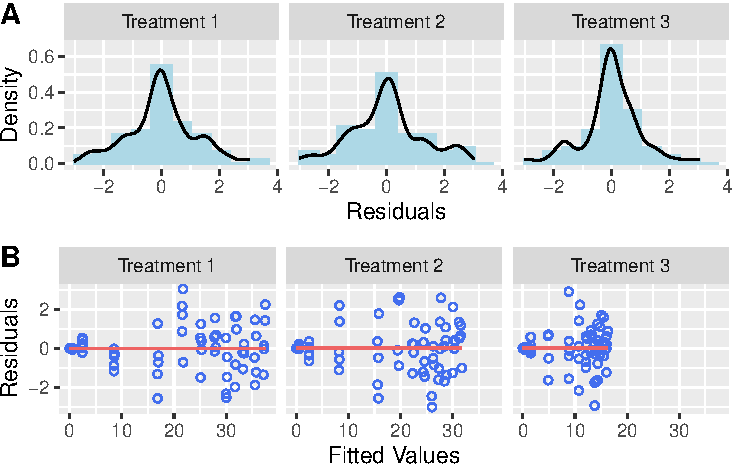
\includegraphics[width=0.8\linewidth,height=\textheight,keepaspectratio]{index_files/mediabag/non-linear_regression_files/figure-pdf/fig-mf-assump-1.pdf}

}

\caption{\label{fig-mf-assump}Histograms (A) of residuals and plots of
residuals vs.~the fitted values (B) for residuals for the three
treatments in the multiple-flask experiment.}

\end{figure}%

The Shapiro-Wilk test results indicate that the residuals are normally
distributed for Treatments 1 and 2 (\emph{p} \textgreater{} 0.05) but
not for Treatment 3 (\emph{p} \textless{} 0.05). However, the histograms
in Figure~\ref{fig-mf-assump} show that the residuals are approximately
normally distributed for all treatment groups, with the median roughly
in the middle of the distribution in each case. This apparent
discrepancy can be explained by the sensitivity of the Shapiro-Wilk test
to sample size. With large sample sizes, even minor deviations from
normality can be detected as statistically significant. In situations
such as this one, I suggest that it is important to consider the sample
size and visual inspection of the data when interpreting the results of
normality tests. Here, given the relatively large sample size and the
visual assessment of the histograms, we can reasonably conclude that the
residuals are approximately normally distributed for all treatment
groups.

Another normality tests such as the Kolmogorov-Smirnov (K-S) test might
be less sensitive to sample size and could be considered for comparison.
The K-S test is a non-parametric statistical test that is used to
determine if a sample comes from a specific probability distribution.
Here I use it to test if a sample follows a normal distribution
(\texttt{pnorm}), but it can also be used to test against other
theoretical distributions or to compare two empirical distributions. The
K-S test can be performed using the \texttt{ks.test()}, as shown below.

\begin{Shaded}
\begin{Highlighting}[]
\NormalTok{perform\_ks\_test }\OtherTok{\textless{}{-}} \ControlFlowTok{function}\NormalTok{(data, treatment) \{}
  \FunctionTok{ks.test}\NormalTok{(data}\SpecialCharTok{$}\NormalTok{residuals\_separate[data}\SpecialCharTok{$}\NormalTok{trt }\SpecialCharTok{==}\NormalTok{ treatment], }\StringTok{"pnorm"}\NormalTok{, }
          \AttributeTok{mean =} \FunctionTok{mean}\NormalTok{(data}\SpecialCharTok{$}\NormalTok{residuals\_separate[data}\SpecialCharTok{$}\NormalTok{trt }\SpecialCharTok{==}\NormalTok{ treatment]), }
          \AttributeTok{sd =} \FunctionTok{sd}\NormalTok{(data}\SpecialCharTok{$}\NormalTok{residuals\_separate[data}\SpecialCharTok{$}\NormalTok{trt }\SpecialCharTok{==}\NormalTok{ treatment]))}
\NormalTok{\}}

\CommentTok{\# Perform the test for each treatment group}
\FunctionTok{perform\_ks\_test}\NormalTok{(mf\_data2, }\StringTok{"Treatment 1"}\NormalTok{)}
\SpecialCharTok{\textgreater{}} 
\ErrorTok{\textgreater{}}\NormalTok{   Asymptotic one}\SpecialCharTok{{-}}\NormalTok{sample Kolmogorov}\SpecialCharTok{{-}}\NormalTok{Smirnov test}
\SpecialCharTok{\textgreater{}} 
\ErrorTok{\textgreater{}}\NormalTok{ data}\SpecialCharTok{:}\NormalTok{  data}\SpecialCharTok{$}\NormalTok{residuals\_separate[data}\SpecialCharTok{$}\NormalTok{trt }\SpecialCharTok{==}\NormalTok{ treatment]}
\SpecialCharTok{\textgreater{}}\NormalTok{ D }\OtherTok{=} \FloatTok{0.10658}\NormalTok{, p}\SpecialCharTok{{-}}\NormalTok{value }\OtherTok{=} \FloatTok{0.4513}
\SpecialCharTok{\textgreater{}}\NormalTok{ alternative hypothesis}\SpecialCharTok{:}\NormalTok{ two}\SpecialCharTok{{-}}\NormalTok{sided}
\FunctionTok{perform\_ks\_test}\NormalTok{(mf\_data2, }\StringTok{"Treatment 2"}\NormalTok{)}
\SpecialCharTok{\textgreater{}} 
\ErrorTok{\textgreater{}}\NormalTok{   Asymptotic one}\SpecialCharTok{{-}}\NormalTok{sample Kolmogorov}\SpecialCharTok{{-}}\NormalTok{Smirnov test}
\SpecialCharTok{\textgreater{}} 
\ErrorTok{\textgreater{}}\NormalTok{ data}\SpecialCharTok{:}\NormalTok{  data}\SpecialCharTok{$}\NormalTok{residuals\_separate[data}\SpecialCharTok{$}\NormalTok{trt }\SpecialCharTok{==}\NormalTok{ treatment]}
\SpecialCharTok{\textgreater{}}\NormalTok{ D }\OtherTok{=} \FloatTok{0.1246}\NormalTok{, p}\SpecialCharTok{{-}}\NormalTok{value }\OtherTok{=} \FloatTok{0.2652}
\SpecialCharTok{\textgreater{}}\NormalTok{ alternative hypothesis}\SpecialCharTok{:}\NormalTok{ two}\SpecialCharTok{{-}}\NormalTok{sided}
\FunctionTok{perform\_ks\_test}\NormalTok{(mf\_data2, }\StringTok{"Treatment 3"}\NormalTok{)}
\SpecialCharTok{\textgreater{}} 
\ErrorTok{\textgreater{}}\NormalTok{   Asymptotic one}\SpecialCharTok{{-}}\NormalTok{sample Kolmogorov}\SpecialCharTok{{-}}\NormalTok{Smirnov test}
\SpecialCharTok{\textgreater{}} 
\ErrorTok{\textgreater{}}\NormalTok{ data}\SpecialCharTok{:}\NormalTok{  data}\SpecialCharTok{$}\NormalTok{residuals\_separate[data}\SpecialCharTok{$}\NormalTok{trt }\SpecialCharTok{==}\NormalTok{ treatment]}
\SpecialCharTok{\textgreater{}}\NormalTok{ D }\OtherTok{=} \FloatTok{0.14151}\NormalTok{, p}\SpecialCharTok{{-}}\NormalTok{value }\OtherTok{=} \FloatTok{0.148}
\SpecialCharTok{\textgreater{}}\NormalTok{ alternative hypothesis}\SpecialCharTok{:}\NormalTok{ two}\SpecialCharTok{{-}}\NormalTok{sided}
\end{Highlighting}
\end{Shaded}

We see that the K-S test indicates that the residuals are normally
distributed for all treatment groups (\emph{p} \textgreater{} 0.05). As
already noted, this test is less sensitive to sample size than the
Shapiro-Wilk test, and the results are consistent with the visual
assessment of the histograms.

We should also check for homoscedasticity (here I use the Levene test)
and a plot of residuals versus fitted values.

\begin{Shaded}
\begin{Highlighting}[]
\CommentTok{\# Perform the Levene test}
\NormalTok{car}\SpecialCharTok{::}\FunctionTok{leveneTest}\NormalTok{(residuals\_separate }\SpecialCharTok{\textasciitilde{}}\NormalTok{ trt, }\AttributeTok{data =}\NormalTok{ mf\_data2)}
\SpecialCharTok{\textgreater{}}\NormalTok{ Levene}\StringTok{\textquotesingle{}s Test for Homogeneity of Variance (center = median)}
\StringTok{\textgreater{}        Df F value Pr(\textgreater{}F)}
\StringTok{\textgreater{} group   2  1.4933 0.2272}
\StringTok{\textgreater{}       192}
\end{Highlighting}
\end{Shaded}

The Levene test shows that the variances are the same across the three
treatments and this is confirmed by the plot of residuals against the
fitted values in Figure~\ref{fig-mf-assump}.

\begin{tcolorbox}[enhanced jigsaw, opacitybacktitle=0.6, toptitle=1mm, colframe=quarto-callout-tip-color-frame, arc=.35mm, left=2mm, rightrule=.15mm, coltitle=black, opacityback=0, bottomrule=.15mm, bottomtitle=1mm, title=\textcolor{quarto-callout-tip-color}{\faLightbulb}\hspace{0.5em}{Results}, toprule=.15mm, colbacktitle=quarto-callout-tip-color!10!white, titlerule=0mm, leftrule=.75mm, colback=white, breakable]

Michaelis-Menten models were fitted to nutrient uptake data across three
experimental treatments to investigate the effects of the treatments on
seaweed nutrient kinetics. A global model, assuming shared kinetic
parameters (\(V_{max}\) and \(K_m\)) across all treatments, was compared
to a model with separate parameters for each treatment. The model
allowing treatment-specific parameters (AIC = 644.3) provided a
significantly better fit to the data than the global model (AIC =
681.5), a finding confirmed by the log-likelihood test (log-likelihood
ratio = 45.20, d.f. = 4, \emph{p} \textless{} 0.0001). As the assumption
tests do not indicate any cause for concern regarding the distribution
of residuals, we conclude that the experimental treatments significantly
influenced the nutrient uptake kinetics of the seaweed
(Figure~\ref{fig-mf3}).

Specifically, all three treatments exhibited unique combinations of
\(V_{max}\) and \(K_m\) values (Treatment 1: \(V_{max}\) = 49.2, \(K_m\)
= 9.5; Treatment 2: \(V_{max}\) = 39.3, \(K_m\) = 7.5; Treatment 3:
\(V_{max}\) = 19.0, \(K_m\) = 5.5). These findings support the
hypothesis that nutrient uptake kinetics in this seaweed species are
sensitive to environmental perturbations.

\end{tcolorbox}

\begin{figure}[t]

\centering{

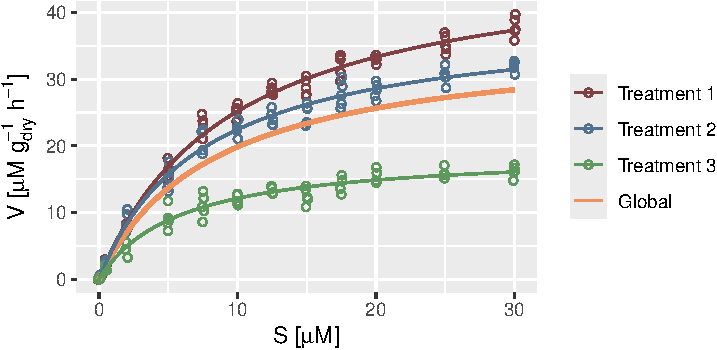
\includegraphics[width=0.8\linewidth,height=\textheight,keepaspectratio]{index_files/mediabag/non-linear_regression_files/figure-pdf/fig-mf3-1.pdf}

}

\caption{\label{fig-mf3}Plot of the Michaelis-Menten model fitted to the
data in Table~\ref{tbl-mf2}. Fits are provided for the separate models
and the global model.}

\end{figure}%

\subsection{The Perturbation Method (NLMM)}\label{sec-perturbation}

The data for this example is by {[}5{]}. A perturbation experiment was
conducted to determine the nutrient uptake rate versus nutrient
concentration of the red seaweed, \emph{Gracilaria} sp. The experiment
involved flasks, initially enriched to approximately 55 μM nitrate,
sampled 16 times over approximately 2.5 hours. The uptake rates were
measured under three rates of water movement (treatments): low, medium,
and high. Each treatment had three replicate flasks
(Table~\ref{tbl-mm1}). The primary objective was to determine if the
Michaelis-Menten parameters significantly differ among the three levels
of water movement, and we must state a hypothesis similar to those in
Section~\ref{sec-mm-comparison}.

\begin{table}

\caption{\label{tbl-mm1}Simulated data for a multiple flask experiment
on an alga (showing only the top and bottom three rows).}

\centering{

\fontsize{12.0pt}{14.4pt}\selectfont
\begin{tabular*}{\linewidth}{@{\extracolsep{\fill}}ccrr}
\toprule
Replicate flask & Treatment & V & [S] \\ 
\midrule\addlinespace[2.5pt]
1 & low & 10.8 & 60.2 \\ 
2 & low & 10.0 & 61.1 \\ 
3 & low & 14.1 & 60.8 \\ 
1 & high & 0.0 & 0.1 \\ 
2 & high & 0.0 & 0.1 \\ 
3 & high & 0.0 & 0.1 \\ 
\bottomrule
\end{tabular*}

}

\end{table}%

For the reasons discussed in Section~\ref{sec-ex1}, we will use a
nonlinear mixed effects model, \texttt{nlme()}, to analyse these data.
Models such as these can be quite challenging to fit. There are several
things we have to deal with. First and most obviously is the fact that
the data are repeated measures, and the residuals may be correlated.
Second, the flasks are nested within the treatment levels, and we need
to account for this in the model. Finally, we need to account for the
possibility that the Michaelis-Menten parameters may vary among the
treatment levels---in fact, we want to test this! Here is the model:

\phantomsection\label{annotated-cell-71}%
\begin{Shaded}
\begin{Highlighting}[]
\CommentTok{\# Determine the number of levels in the factor \textquotesingle{}trt\textquotesingle{}}
\NormalTok{num\_levels }\OtherTok{\textless{}{-}} \FunctionTok{length}\NormalTok{(}\FunctionTok{levels}\NormalTok{(mm\_data}\SpecialCharTok{$}\NormalTok{trt))}

\CommentTok{\# Starting values for the fixed parameters}
\CommentTok{\# (one set for each level of \textquotesingle{}trt\textquotesingle{})}
\NormalTok{start\_vals }\OtherTok{\textless{}{-}} \FunctionTok{list}\NormalTok{(}\AttributeTok{fixed =} \FunctionTok{c}\NormalTok{(}\AttributeTok{Vmax =} \FunctionTok{rep}\NormalTok{(}\FunctionTok{max}\NormalTok{(mm\_data}\SpecialCharTok{$}\NormalTok{V), num\_levels),}
                             \AttributeTok{Km =} \FunctionTok{rep}\NormalTok{(}\FunctionTok{median}\NormalTok{(mm\_data}\SpecialCharTok{$}\NormalTok{S), num\_levels)))}

\NormalTok{nlme\_mod2 }\OtherTok{\textless{}{-}} \FunctionTok{nlme}\NormalTok{(V }\SpecialCharTok{\textasciitilde{}} \FunctionTok{mm\_fun}\NormalTok{(S, Vmax, Km),}
                  \AttributeTok{data =}\NormalTok{ mm\_data,}
                  \AttributeTok{fixed =}\NormalTok{ Vmax }\SpecialCharTok{+}\NormalTok{ Km }\SpecialCharTok{\textasciitilde{}}\NormalTok{ trt, }\hspace*{\fill}\NormalTok{\circled{1}}
                  \AttributeTok{random =}\NormalTok{ Vmax }\SpecialCharTok{+}\NormalTok{ Km }\SpecialCharTok{\textasciitilde{}} \DecValTok{1} \SpecialCharTok{|}\NormalTok{ flask, }\hspace*{\fill}\NormalTok{\circled{2}}
                  \AttributeTok{start =}\NormalTok{ start\_vals,}
                  \AttributeTok{method =} \StringTok{"REML"}\NormalTok{)}
\end{Highlighting}
\end{Shaded}

\begin{description}
\tightlist
\item[\circled{1}]
The \texttt{fixed} argument specifies that the Michaelis-Menten
parameters \texttt{Vmax} and \texttt{Km} are fixed effects that vary
among the treatment levels, and a grouping variable (\texttt{trt}) is
used to specify the levels of the treatment factor.
\item[\circled{2}]
The \texttt{random} argument specifies that the Michaelis-Menten
parameters \texttt{Vmax} and \texttt{Km} are random effects that vary
among the replicate flasks.
\end{description}

This model brings us closer to our goal, but there are some notable
omissions. The specification allows the Michaelis-Menten parameters to
vary among the treatment levels, which is central to our hypothesis. We
have also accounted for the replication structure of the data,
recognising that random variations may arise not due to the treatment
levels but due to the replicate flasks.

However, we have not accounted for the central feature of a perturbation
experiment, which is the correlation structure of the residuals. We must
deal with the fact that the residuals may be correlated due to the
repeated measures nature of the data. Additionally, we have omitted the
nesting of the flasks within the treatment levels.

Let's update our model accordingly:

\phantomsection\label{annotated-cell-72}%
\begin{Shaded}
\begin{Highlighting}[]
\NormalTok{nlme\_mod3 }\OtherTok{\textless{}{-}} \FunctionTok{nlme}\NormalTok{(V }\SpecialCharTok{\textasciitilde{}} \FunctionTok{mm\_fun}\NormalTok{(S, Vmax, Km),}
                  \AttributeTok{data =}\NormalTok{ mm\_data,}
                  \AttributeTok{fixed =} \FunctionTok{list}\NormalTok{(Vmax }\SpecialCharTok{\textasciitilde{}}\NormalTok{ trt, Km }\SpecialCharTok{\textasciitilde{}}\NormalTok{ trt),}
                  \AttributeTok{random =}\NormalTok{ Vmax }\SpecialCharTok{\textasciitilde{}} \DecValTok{1} \SpecialCharTok{|}\NormalTok{ trt}\SpecialCharTok{/}\NormalTok{flask, }\hspace*{\fill}\NormalTok{\circled{1}}
                  \AttributeTok{groups =} \SpecialCharTok{\textasciitilde{}}\NormalTok{ trt}\SpecialCharTok{/}\NormalTok{flask, }\hspace*{\fill}\NormalTok{\circled{2}}
                  \AttributeTok{correlation =} \FunctionTok{corAR1}\NormalTok{(}\AttributeTok{form =} \SpecialCharTok{\textasciitilde{}} \DecValTok{1} \SpecialCharTok{|}\NormalTok{ trt}\SpecialCharTok{/}\NormalTok{flask), }\hspace*{\fill}\NormalTok{\circled{3}}
                  \AttributeTok{start =}\NormalTok{ start\_vals,}
                  \AttributeTok{method =} \StringTok{"REML"}\NormalTok{)}
\end{Highlighting}
\end{Shaded}

\begin{description}
\tightlist
\item[\circled{1}]
The \texttt{random} argument specifies that the Michaelis-Menten
parameter \texttt{Vmax} is a random effect that varies among the
replicate flasks nested within the treatment levels.
\item[\circled{2}]
The \texttt{groups} argument specifies that the replicate flasks are
nested within the treatment levels.
\item[\circled{3}]
The \texttt{correlation} argument specifies that the residuals have a
first-order autoregressive correlation structure. This structure assumes
that the correlation between residuals decreases exponentially with the
time lag between observations. Flask is nested \emph{within} treatment.
\end{description}

If we are not convinced that \texttt{nlme\_mod3} is the best model, we
can compare it to \texttt{nlme\_mod2} using a likelihood ratio test. It
is used to compare the fit of two models, where one model is a special
case of the other. The test statistic is the difference in the
log-likelihoods of the two models, and the null hypothesis is that the
simpler model is the best fit.

\begin{Shaded}
\begin{Highlighting}[]
\FunctionTok{anova}\NormalTok{(nlme\_mod2, nlme\_mod3)}
\SpecialCharTok{\textgreater{}}\NormalTok{           Model df      AIC      BIC    logLik}
\SpecialCharTok{\textgreater{}}\NormalTok{ nlme\_mod2     }\DecValTok{1} \DecValTok{10} \FloatTok{637.2782} \FloatTok{665.6411} \SpecialCharTok{{-}}\FloatTok{308.6391}
\SpecialCharTok{\textgreater{}}\NormalTok{ nlme\_mod3     }\DecValTok{2} \DecValTok{10} \FloatTok{632.1053} \FloatTok{660.4681} \SpecialCharTok{{-}}\FloatTok{306.0527}

\CommentTok{\# Likelihood ratio test}
\NormalTok{lrt\_stat }\OtherTok{\textless{}{-}} \SpecialCharTok{{-}}\DecValTok{2} \SpecialCharTok{*}\NormalTok{ (}\FunctionTok{logLik}\NormalTok{(nlme\_mod2) }\SpecialCharTok{{-}} \FunctionTok{logLik}\NormalTok{(nlme\_mod3))}

\CommentTok{\# Determine degrees of freedom and p{-}value}
\NormalTok{df\_diff }\OtherTok{\textless{}{-}} \FunctionTok{attr}\NormalTok{(}\FunctionTok{logLik}\NormalTok{(nlme\_mod3), }\StringTok{"df"}\NormalTok{) }\SpecialCharTok{{-}} \FunctionTok{attr}\NormalTok{(}\FunctionTok{logLik}\NormalTok{(nlme\_mod2), }\StringTok{"df"}\NormalTok{) }
\NormalTok{p\_value }\OtherTok{\textless{}{-}} \FunctionTok{pchisq}\NormalTok{(lrt\_stat, }\AttributeTok{df =}\NormalTok{ df\_diff, }\AttributeTok{lower.tail =} \ConstantTok{FALSE}\NormalTok{) }

\FunctionTok{print}\NormalTok{(}\FunctionTok{paste}\NormalTok{(}\StringTok{"LRT statistic:"}\NormalTok{, lrt\_stat))}
\SpecialCharTok{\textgreater{}}\NormalTok{ [}\DecValTok{1}\NormalTok{] }\StringTok{"LRT statistic: 5.17293584867423"}
\FunctionTok{print}\NormalTok{(}\FunctionTok{paste}\NormalTok{(}\StringTok{"Degrees of freedom:"}\NormalTok{, df\_diff))}
\SpecialCharTok{\textgreater{}}\NormalTok{ [}\DecValTok{1}\NormalTok{] }\StringTok{"Degrees of freedom: 0"}
\FunctionTok{print}\NormalTok{(}\FunctionTok{paste}\NormalTok{(}\StringTok{"P{-}value:"}\NormalTok{, p\_value))}
\SpecialCharTok{\textgreater{}}\NormalTok{ [}\DecValTok{1}\NormalTok{] }\StringTok{"P{-}value: 0"}
\end{Highlighting}
\end{Shaded}

The likelihood ratio test indicates that \texttt{nlme\_mod3} is a better
fit than \texttt{nlme\_mod2} (\emph{p} \textless{} 0.001). This result
suggests that the Michaelis-Menten parameters vary among the treatment
levels, and the residuals have a first-order autoregressive correlation
structure.

\begin{Shaded}
\begin{Highlighting}[]
\FunctionTok{summary}\NormalTok{(nlme\_mod3)}
\SpecialCharTok{\textgreater{}}\NormalTok{ Nonlinear mixed}\SpecialCharTok{{-}}\NormalTok{effects model fit by REML}
\SpecialCharTok{\textgreater{}}\NormalTok{   Model}\SpecialCharTok{:}\NormalTok{ V }\SpecialCharTok{\textasciitilde{}} \FunctionTok{mm\_fun}\NormalTok{(S, Vmax, Km) }
\SpecialCharTok{\textgreater{}}\NormalTok{   Data}\SpecialCharTok{:}\NormalTok{ mm\_data }
\SpecialCharTok{\textgreater{}}\NormalTok{        AIC      BIC    logLik}
\SpecialCharTok{\textgreater{}}   \FloatTok{632.1053} \FloatTok{660.4681} \SpecialCharTok{{-}}\FloatTok{306.0527}
\SpecialCharTok{\textgreater{}} 
\ErrorTok{\textgreater{}}\NormalTok{ Random effects}\SpecialCharTok{:}
\ErrorTok{\textgreater{}}\NormalTok{  Formula}\SpecialCharTok{:}\NormalTok{ Vmax }\SpecialCharTok{\textasciitilde{}} \DecValTok{1} \SpecialCharTok{|}\NormalTok{ trt}
\SpecialCharTok{\textgreater{}}         \FunctionTok{Vmax.}\NormalTok{(Intercept)}
\SpecialCharTok{\textgreater{}}\NormalTok{ StdDev}\SpecialCharTok{:}       \FloatTok{0.00837941}
\SpecialCharTok{\textgreater{}} 
\ErrorTok{\textgreater{}}\NormalTok{  Formula}\SpecialCharTok{:}\NormalTok{ Vmax }\SpecialCharTok{\textasciitilde{}} \DecValTok{1} \SpecialCharTok{|}\NormalTok{ flask }\SpecialCharTok{\%in\%}\NormalTok{ trt}
\SpecialCharTok{\textgreater{}}         \FunctionTok{Vmax.}\NormalTok{(Intercept) Residual}
\SpecialCharTok{\textgreater{}}\NormalTok{ StdDev}\SpecialCharTok{:}     \FloatTok{0.0002584018} \FloatTok{2.731378}
\SpecialCharTok{\textgreater{}} 
\ErrorTok{\textgreater{}}\NormalTok{ Correlation Structure}\SpecialCharTok{:} \FunctionTok{AR}\NormalTok{(}\DecValTok{1}\NormalTok{)}
\SpecialCharTok{\textgreater{}}\NormalTok{  Formula}\SpecialCharTok{:} \ErrorTok{\textasciitilde{}}\DecValTok{1} \SpecialCharTok{|}\NormalTok{ trt}\SpecialCharTok{/}\NormalTok{flask }
\SpecialCharTok{\textgreater{}}\NormalTok{  Parameter }\FunctionTok{estimate}\NormalTok{(s)}\SpecialCharTok{:}
\ErrorTok{\textgreater{}}\NormalTok{       Phi }
\SpecialCharTok{\textgreater{}} \FloatTok{0.2048944} 
\SpecialCharTok{\textgreater{}}\NormalTok{ Fixed effects}\SpecialCharTok{:}  \FunctionTok{list}\NormalTok{(Vmax }\SpecialCharTok{\textasciitilde{}}\NormalTok{ trt, Km }\SpecialCharTok{\textasciitilde{}}\NormalTok{ trt) }
\SpecialCharTok{\textgreater{}}\NormalTok{                      Value Std.Error  DF   t}\SpecialCharTok{{-}}\NormalTok{value p}\SpecialCharTok{{-}}\NormalTok{value}
\SpecialCharTok{\textgreater{}} \FunctionTok{Vmax.}\NormalTok{(Intercept) }\FloatTok{15.394469}  \FloatTok{1.082697} \DecValTok{118} \FloatTok{14.218627}  \FloatTok{0.0000}
\SpecialCharTok{\textgreater{}}\NormalTok{ Vmax.trtlow      }\SpecialCharTok{{-}}\FloatTok{1.660245}  \FloatTok{2.381505} \DecValTok{118} \SpecialCharTok{{-}}\FloatTok{0.697141}  \FloatTok{0.4871}
\SpecialCharTok{\textgreater{}}\NormalTok{ Vmax.trtmed      }\SpecialCharTok{{-}}\FloatTok{3.555246}  \FloatTok{1.503682} \DecValTok{118} \SpecialCharTok{{-}}\FloatTok{2.364361}  \FloatTok{0.0197}
\SpecialCharTok{\textgreater{}} \FunctionTok{Km.}\NormalTok{(Intercept)    }\FloatTok{5.381378}  \FloatTok{1.873000} \DecValTok{118}  \FloatTok{2.873133}  \FloatTok{0.0048}
\SpecialCharTok{\textgreater{}}\NormalTok{ Km.trtlow        }\FloatTok{11.448682}  \FloatTok{8.044641} \DecValTok{118}  \FloatTok{1.423144}  \FloatTok{0.1573}
\SpecialCharTok{\textgreater{}}\NormalTok{ Km.trtmed        }\SpecialCharTok{{-}}\FloatTok{0.381246}  \FloatTok{3.147606} \DecValTok{118} \SpecialCharTok{{-}}\FloatTok{0.121123}  \FloatTok{0.9038}
\SpecialCharTok{\textgreater{}}\NormalTok{  Correlation}\SpecialCharTok{:} 
\ErrorTok{\textgreater{}}                \FunctionTok{Vm.}\NormalTok{(I) Vmx.trtl Vmx.trtm }\FunctionTok{Km.}\NormalTok{(I) Km.trtl}
\SpecialCharTok{\textgreater{}}\NormalTok{ Vmax.trtlow    }\SpecialCharTok{{-}}\FloatTok{0.455}                                 
\SpecialCharTok{\textgreater{}}\NormalTok{ Vmax.trtmed    }\SpecialCharTok{{-}}\FloatTok{0.720}  \FloatTok{0.327}                          
\SpecialCharTok{\textgreater{}} \FunctionTok{Km.}\NormalTok{(Intercept)  }\FloatTok{0.726} \SpecialCharTok{{-}}\FloatTok{0.330}   \SpecialCharTok{{-}}\FloatTok{0.523}                 
\SpecialCharTok{\textgreater{}}\NormalTok{ Km.trtlow      }\SpecialCharTok{{-}}\FloatTok{0.169}  \FloatTok{0.876}    \FloatTok{0.122}   \SpecialCharTok{{-}}\FloatTok{0.233}        
\SpecialCharTok{\textgreater{}}\NormalTok{ Km.trtmed      }\SpecialCharTok{{-}}\FloatTok{0.432}  \FloatTok{0.196}    \FloatTok{0.734}   \SpecialCharTok{{-}}\FloatTok{0.595}  \FloatTok{0.139} 
\SpecialCharTok{\textgreater{}} 
\ErrorTok{\textgreater{}}\NormalTok{ Standardized Within}\SpecialCharTok{{-}}\NormalTok{Group Residuals}\SpecialCharTok{:}
\ErrorTok{\textgreater{}}\NormalTok{        Min         Q1        Med         Q3        Max }
\SpecialCharTok{\textgreater{}} \SpecialCharTok{{-}}\FloatTok{2.0222398} \SpecialCharTok{{-}}\FloatTok{0.7529003} \SpecialCharTok{{-}}\FloatTok{0.2362146}  \FloatTok{0.4364407}  \FloatTok{3.2055101} 
\SpecialCharTok{\textgreater{}} 
\ErrorTok{\textgreater{}}\NormalTok{ Number of Observations}\SpecialCharTok{:} \DecValTok{132}
\SpecialCharTok{\textgreater{}}\NormalTok{ Number of Groups}\SpecialCharTok{:} 
\ErrorTok{\textgreater{}}\NormalTok{            trt flask }\SpecialCharTok{\%in\%}\NormalTok{ trt }
\SpecialCharTok{\textgreater{}}              \DecValTok{3}              \DecValTok{9}
\end{Highlighting}
\end{Shaded}

\section{Example: The Growth Rate of Fish
(NLMM)}\label{sec-vonbertalanffy}

The von Bertalanffy model (Equation~\ref{eq-vb}) is used to describe the
growth patterns of animals over time. For example, in a fish growth
study, we measure the length of individual fish at regular intervals as
the fish ages. We can estimate growth parameters specific to the fish
species by fitting the von Bertalanffy model to these length-at-age data

The model is given by:

\begin{equation}\phantomsection\label{eq-vb}{L(t) = L_{\infty} \left(1 - e^{-k(t-t_0)}\right)}\end{equation}

Where:

\begin{itemize}
\tightlist
\item
  \(L(t)\) is the length of the fish at time \(t\).
\item
  \(L_{\infty}\) is the asymptotic length, representing the theoretical
  maximum length that the individual would reach if it grew
  indefinitely.
\item
  \(k\) is the growth coefficient, indicating the rate at which the
  growth of the fish approaches its maximum size. A higher \(k\) value
  means it reaches its asymptotic length more quickly.
\item
  \(t_0\) is the hypothetical age at which the individual's length would
  be zero according to the model.
\end{itemize}

\(L_{\infty}\) (the asymptotic length) represents the length towards
which the individual grows as time (\(t\)) approaches infinity. The
concept behind \(L_{\infty}\) is that as the fish ages, its growth rate
slows down and eventually approaches zero, with its length nearing the
asymptotic value \(L_{\infty}\). \(k\) (the growth rate coefficient)
determines how quickly the fish reaches its asymptotic length.
Physiologically, \(k\) reflects the metabolic rates and general fitness
of the fish, while ecologically, it can be influenced by environmental
factors such as food availability and temperature. Lastly, \(t_0\) (the
theoretical age at zero length) is not directly observable in practice
but provides a useful way to shift the growth curve along the time axis
to provide a better fit to the data, especially in the early
developmental stages.

Consider a study where the lengths of 30 Atlantic Cod, \emph{Gadus
morua}, in captivity are measured twice a year from hatching to 15
years. This creates a longitudinal dataset with repeated length
measurements for each fish over time. In this experiment, we will focus
on the growth patterns of individual fish, assuming they were raised
under identical conditions. This allows us to attribute any growth
differences to inherent biological variation among the fish. Apart from
the repeated measures on individual fish, we will assume that the data
are independent in all other respects.

The longitudinal nature of the data requires that we use appropriate
statistical methods that account for the correlation among the repeated
measures. We will use a nonlinear mixed-effects regression for the data
in Table 1.

\begin{table}
\caption{The Atlantic Cod data set with 30 fish and 15 years of growth data
(showing only the top and bottom three rows).}\tabularnewline

\fontsize{12.0pt}{14.4pt}\selectfont
\begin{tabular*}{\linewidth}{@{\extracolsep{\fill}}ccc}
\toprule
Fish ID & Age (yr) & Length (cm) \\ 
\midrule\addlinespace[2.5pt]
1 & 0.0 & 5.3 \\ 
1 & 0.5 & 16.8 \\ 
1 & 1.0 & 27.2 \\ 
30 & 14.0 & 115.4 \\ 
30 & 14.5 & 116.0 \\ 
30 & 15.0 & 116.5 \\ 
\bottomrule
\end{tabular*}
\end{table}

A plot of the data is shown in Figure~\ref{fig-vb1}; here, each line
represents the growth trajectory of an individual fish over time.

\begin{verbatim}
> List of 1
>  $ legend.position: chr "none"
>  - attr(*, "class")= chr [1:2] "theme" "gg"
>  - attr(*, "complete")= logi FALSE
>  - attr(*, "validate")= logi TRUE
\end{verbatim}

\begin{figure}[tbp]

\centering{

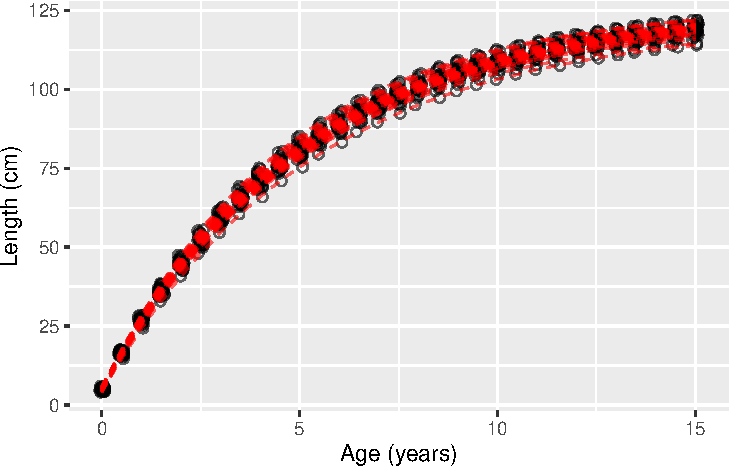
\includegraphics[width=0.8\linewidth,height=\textheight,keepaspectratio]{index_files/mediabag/non-linear_regression_files/figure-pdf/fig-vb1-1.pdf}

}

\caption{\label{fig-vb1}Plot of growth data measured in 30 Atlantic cod,
\emph{Gadus morua}.}

\end{figure}%

We will fit the von Bertalanffy growth model to the data using
\texttt{nlme::nlme()} as follows, and the output is provided:

\phantomsection\label{annotated-cell-75}%
\begin{Shaded}
\begin{Highlighting}[]
\CommentTok{\# von Bertalanffy growth function}
\NormalTok{vb\_growth }\OtherTok{\textless{}{-}} \ControlFlowTok{function}\NormalTok{(age, L\_inf, k, t0) \{}
\NormalTok{  L\_inf }\SpecialCharTok{*}\NormalTok{ (}\DecValTok{1} \SpecialCharTok{{-}} \FunctionTok{exp}\NormalTok{(}\SpecialCharTok{{-}}\NormalTok{k }\SpecialCharTok{*}\NormalTok{ (age }\SpecialCharTok{{-}}\NormalTok{ t0)))}
\NormalTok{\}}

\CommentTok{\# Define the nonlinear mixed{-}effects model}
\NormalTok{nlme\_model }\OtherTok{\textless{}{-}} \FunctionTok{nlme}\NormalTok{(Length }\SpecialCharTok{\textasciitilde{}} \FunctionTok{vb\_growth}\NormalTok{(Age, L\_inf, k, t0),}
                   \AttributeTok{data =}\NormalTok{ vb\_data,}
                   \AttributeTok{fixed =}\NormalTok{ L\_inf }\SpecialCharTok{+}\NormalTok{ k }\SpecialCharTok{+}\NormalTok{ t0 }\SpecialCharTok{\textasciitilde{}} \DecValTok{1}\NormalTok{, }\hspace*{\fill}\NormalTok{\circled{1}}
                   \AttributeTok{random =}\NormalTok{ L\_inf }\SpecialCharTok{+}\NormalTok{ k }\SpecialCharTok{\textasciitilde{}} \DecValTok{1} \SpecialCharTok{|}\NormalTok{ Fish\_ID, }\hspace*{\fill}\NormalTok{\circled{2}}
                   \AttributeTok{groups =} \SpecialCharTok{\textasciitilde{}}\NormalTok{ Fish\_ID, }\hspace*{\fill}\NormalTok{\circled{3}}
                   \AttributeTok{correlation =} \FunctionTok{corAR1}\NormalTok{(}\AttributeTok{form =} \SpecialCharTok{\textasciitilde{}} \DecValTok{1}\NormalTok{), }\hspace*{\fill}\NormalTok{\circled{4}}
                   \AttributeTok{start =} \FunctionTok{c}\NormalTok{(}\AttributeTok{L\_inf =} \DecValTok{100}\NormalTok{, }\AttributeTok{k =} \FloatTok{0.2}\NormalTok{, }\AttributeTok{t0 =} \SpecialCharTok{{-}}\FloatTok{0.5}\NormalTok{))}

\CommentTok{\# Print the summary of the model}
\FunctionTok{summary}\NormalTok{(nlme\_model)}
\SpecialCharTok{\textgreater{}}\NormalTok{ Nonlinear mixed}\SpecialCharTok{{-}}\NormalTok{effects model fit by maximum likelihood}
\SpecialCharTok{\textgreater{}}\NormalTok{   Model}\SpecialCharTok{:}\NormalTok{ Length }\SpecialCharTok{\textasciitilde{}} \FunctionTok{vb\_growth}\NormalTok{(Age, L\_inf, k, t0) }
\SpecialCharTok{\textgreater{}}\NormalTok{   Data}\SpecialCharTok{:}\NormalTok{ vb\_data }
\SpecialCharTok{\textgreater{}}\NormalTok{         AIC       BIC  logLik}
\SpecialCharTok{\textgreater{}}   \SpecialCharTok{{-}}\FloatTok{2833.361} \SpecialCharTok{{-}}\FloatTok{2794.679} \FloatTok{1424.68}
\SpecialCharTok{\textgreater{}} 
\ErrorTok{\textgreater{}}\NormalTok{ Random effects}\SpecialCharTok{:}
\ErrorTok{\textgreater{}}\NormalTok{  Formula}\SpecialCharTok{:} \FunctionTok{list}\NormalTok{(L\_inf }\SpecialCharTok{\textasciitilde{}} \DecValTok{1}\NormalTok{, k }\SpecialCharTok{\textasciitilde{}} \DecValTok{1}\NormalTok{)}
\SpecialCharTok{\textgreater{}}\NormalTok{  Level}\SpecialCharTok{:}\NormalTok{ Fish\_ID}
\SpecialCharTok{\textgreater{}}\NormalTok{  Structure}\SpecialCharTok{:}\NormalTok{ General positive}\SpecialCharTok{{-}}\NormalTok{definite, Log}\SpecialCharTok{{-}}\NormalTok{Cholesky parametrization}
\SpecialCharTok{\textgreater{}}\NormalTok{          StdDev      Corr  }
\SpecialCharTok{\textgreater{}}\NormalTok{ L\_inf    }\FloatTok{1.857032547}\NormalTok{ L\_inf }
\SpecialCharTok{\textgreater{}}\NormalTok{ k        }\FloatTok{0.008341198} \SpecialCharTok{{-}}\FloatTok{0.139}
\SpecialCharTok{\textgreater{}}\NormalTok{ Residual }\FloatTok{0.555742464}       
\SpecialCharTok{\textgreater{}} 
\ErrorTok{\textgreater{}}\NormalTok{ Correlation Structure}\SpecialCharTok{:} \FunctionTok{AR}\NormalTok{(}\DecValTok{1}\NormalTok{)}
\SpecialCharTok{\textgreater{}}\NormalTok{  Formula}\SpecialCharTok{:} \ErrorTok{\textasciitilde{}}\DecValTok{1} \SpecialCharTok{|}\NormalTok{ Fish\_ID }
\SpecialCharTok{\textgreater{}}\NormalTok{  Parameter }\FunctionTok{estimate}\NormalTok{(s)}\SpecialCharTok{:}
\ErrorTok{\textgreater{}}\NormalTok{       Phi }
\SpecialCharTok{\textgreater{}} \FloatTok{0.9972623} 
\SpecialCharTok{\textgreater{}}\NormalTok{ Fixed effects}\SpecialCharTok{:}\NormalTok{  L\_inf }\SpecialCharTok{+}\NormalTok{ k }\SpecialCharTok{+}\NormalTok{ t0 }\SpecialCharTok{\textasciitilde{}} \DecValTok{1} 
\SpecialCharTok{\textgreater{}}\NormalTok{           Value Std.Error  DF  t}\SpecialCharTok{{-}}\NormalTok{value p}\SpecialCharTok{{-}}\NormalTok{value}
\SpecialCharTok{\textgreater{}}\NormalTok{ L\_inf }\FloatTok{124.80230} \FloatTok{0.3551041} \DecValTok{898} \FloatTok{351.4527}       \DecValTok{0}
\SpecialCharTok{\textgreater{}}\NormalTok{ k       }\FloatTok{0.20042} \FloatTok{0.0015299} \DecValTok{898} \FloatTok{131.0050}       \DecValTok{0}
\SpecialCharTok{\textgreater{}}\NormalTok{ t0     }\SpecialCharTok{{-}}\FloatTok{0.20415} \FloatTok{0.0040574} \DecValTok{898} \SpecialCharTok{{-}}\FloatTok{50.3164}       \DecValTok{0}
\SpecialCharTok{\textgreater{}}\NormalTok{  Correlation}\SpecialCharTok{:} 
\ErrorTok{\textgreater{}}\NormalTok{    L\_inf  k     }
\SpecialCharTok{\textgreater{}}\NormalTok{ k  }\SpecialCharTok{{-}}\FloatTok{0.137}       
\SpecialCharTok{\textgreater{}}\NormalTok{ t0 }\SpecialCharTok{{-}}\FloatTok{0.260} \SpecialCharTok{{-}}\FloatTok{0.007}
\SpecialCharTok{\textgreater{}} 
\ErrorTok{\textgreater{}}\NormalTok{ Standardized Within}\SpecialCharTok{{-}}\NormalTok{Group Residuals}\SpecialCharTok{:}
\ErrorTok{\textgreater{}}\NormalTok{        Min         Q1        Med         Q3        Max }
\SpecialCharTok{\textgreater{}} \SpecialCharTok{{-}}\FloatTok{2.2053004} \SpecialCharTok{{-}}\FloatTok{0.7552048}  \FloatTok{0.2402975}  \FloatTok{0.4902483}  \FloatTok{1.9150860} 
\SpecialCharTok{\textgreater{}} 
\ErrorTok{\textgreater{}}\NormalTok{ Number of Observations}\SpecialCharTok{:} \DecValTok{930}
\SpecialCharTok{\textgreater{}}\NormalTok{ Number of Groups}\SpecialCharTok{:} \DecValTok{30}
\end{Highlighting}
\end{Shaded}

\begin{description}
\tightlist
\item[\circled{1}]
The fixed effects are the parameters of the von Bertalanffy growth model
which are invariant among fish.
\item[\circled{2}]
The random effects are the asymptotic length and growth rate to account
for the intrinsic differences among fish.
\item[\circled{3}]
The grouping variable is the fish ID.
\item[\circled{4}]
The correlation structure is autoregressive of order 1 to account for
the correlation among repeated measures within the same fish, the
\texttt{\textasciitilde{}\ 1} indicates that the order of the
observations in the data must be used along which measurements are
serially correlated, and since no grouping variable is provided, all
fish will have the same correlation structure.
\end{description}

\begin{figure}[tbp]

\centering{

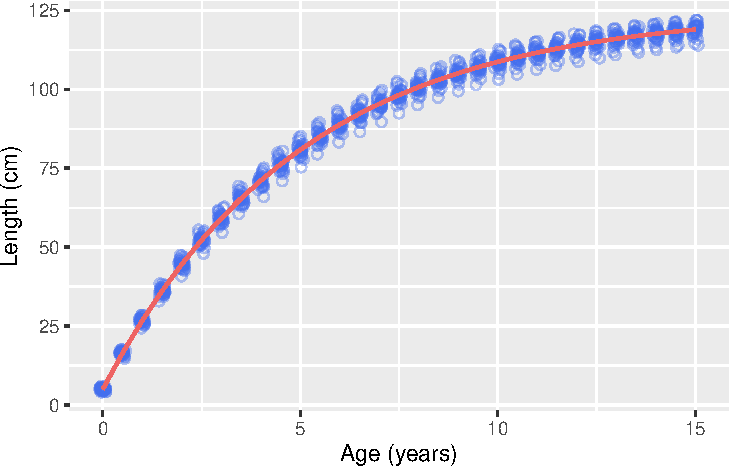
\includegraphics[width=0.8\linewidth,height=\textheight,keepaspectratio]{index_files/mediabag/non-linear_regression_files/figure-pdf/fig-vb2-1.pdf}

}

\caption{\label{fig-vb2}Fit of the von Bertalanffy model to experimental
data obtained from 30 Atlantic Cod individuals.}

\end{figure}%

\section{Scrathpad}\label{scrathpad}

\subsection{To include in the article}\label{to-include-in-the-article}

\begin{itemize}
\tightlist
\item
  \textbf{Assumptions:} Not necessary for simply estimating model
  parameters, but if the model is used for prediction or inference, it
  is important to state the assumptions of the model (e.g., linearity,
  homoscedasticity, independence of residuals) and test them.
\item
  \textbf{i.i.d:} The residuals are assumed to be independent and
  identically distributed (i.i.d.), which is a common assumption in
  linear regression models. For a normal distribution, this is written
  as \(\epsilon_i \sim N(0, \sigma^2)\), where \(\sigma^2\) is the
  variance of the residuals.
\end{itemize}

\subsection{Contuinuing the MM model}\label{contuinuing-the-mm-model}

\chapter{Regularisation Techniques}\label{sec-regularisation}

Regularisation techniques are invaluable when dealing with complex
datasets or situations where traditional methods may fall short. They
are used to enhance model stability, improve predictive performance, and
increase interpretability, especially when working with
multi-dimensional data in multiple linear regression models and
multivariate analyses. Regularisation addresses several common
challenges in statistical modelling: i) multicollinearity, ii) variable
selection, iii) overfitting, and iv) model simplification.

Environmental datasets often contain many independent variables, and it
is likely that only some of them are necessary to explain the phenomenon
of interest. \textbf{Variable selection} is the process of identifying
the most important predictors to include in a model. This can be
achieved through the application of specialist, domain-specific
knowledge, or through statistical or data-driven approaches.
Regularisation is an example of the latter, as it can automatically
identify the most relevant predictors on statistical grounds, serving as
an alternative to traditional variable selection methods such as
Variance Inflation Factor (VIF) and stepwise selection (see
Section~\ref{sec-multicollinearity} and
Section~\ref{sec-forward-selection}).

\textbf{Overfitting} occurs when a model `explains' the noise in data
together with the underlying pattern, which might happen when the model
has too many predictors relative to the number of observations. This may
also result when variable selection has not been sufficiently addressed.
An overfit model performs exceptionally well on training data but fails
to generalise to new, unseen data. Additionally, having too many
predictors can lead to \textbf{multicollinearity} (see
Section~\ref{sec-multicollinearity}). This is a common issue in multiple
linear regression when some of the many predictors included in the model
are correlated. Multicollinearity can lead to inflated standard errors,
unstable coefficients, and difficulty interpreting the model.
Regularisation help manage multicollinearity by shrinking coefficient
estimates or setting some to zero.

Effectiveness in variable selection, reducing multicollinearity, and
mitigating overfitting all contribute to \textbf{model simplification}.
Regularisation achieves similar outcomes by shrinking coefficient
estimates or setting some to zero, making the model easier to
understand, explain, and interpret.

In this chapter, we will discuss three common regularisation techniques:
Lasso, Ridge, and Elastic Net Regression.

\section{Ridge Regression (L2
Regularisation)}\label{ridge-regression-l2-regularisation}

Ridge regression mathematically `tames' the wildness of linear
regression when faced with multicollinearity. It achieves this by adding
a penalty term to the linear regression loss function---a term
proportional to the square of the coefficients (the L2 norm). This
penalty nudges the coefficients towards zero, effectively shrinking them
without forcing them to be exactly zero.

In linear regression, the loss function is typically the Mean Squared
Error (MSE), which is the average of the squared residuals (also known
as the residual sum of squares, RSS). The optimisation objective is to
minimise this loss function. In other words, the linear regression model
aims to find the coefficients that minimise the average squared
difference between the observed values and the predicted values. The RSS
is expressed in Equation~\ref{eq-rss}:

\begin{equation}\phantomsection\label{eq-rss}{RSS(\beta) = \sum_{i=1}^{n} (y_i - \beta_0 - \sum_{j=1}^{p} \beta_j x_{ij})^2}\end{equation}

And the MSE, which is the loss function to be minimised, is in
Equation~\ref{eq-mse}:

\begin{equation}\phantomsection\label{eq-mse}{MSE(\beta) = \frac{1}{n} \sum_{i=1}^{n} (y_i - \beta_0 - \sum_{j=1}^{p} \beta_j x_{ij})^2}\end{equation}

Where:

\begin{itemize}
\tightlist
\item
  \(y_i\) is the observed value for the \(i\)-th observation.
\item
  \(\beta_0\) is the intercept.
\item
  \(\beta_j\) are the coefficients for the predictors.
\item
  \(x_{ij}\) is the value of the \(j\)-th predictor variable for the
  \(i\)-th observation.
\item
  \(n\) is the number of observations.
\item
  \(p\) is the number of predictors.
\end{itemize}

The notation \(RSS(\beta)\) and \(MSE(\beta)\) indicates that these are
functions of the coefficients \(\beta\). The optimisation objective for
linear regression is to find the coefficients \(\beta_0\) and
\(\beta_1\) to \(\beta_p\) that minimise the MSE. This can be expressed
in Equation Equation~\ref{eq-linear-minimisation}:

\begin{equation}\phantomsection\label{eq-linear-minimisation}{\min_{\beta} \left\{ \frac{1}{n} \sum_{i=1}^n (y_i - \beta_0 - \sum_{j=1}^p \beta_j x_{ij})^2 \right\}}\end{equation}

Ridge regression extends the optimisation of the least squares
regression by introducing a penalty term to the loss function. This
penalty term is proportional to the square of the L2 norm of the
coefficient vector, penalising large coefficient values. Ridge
regression is specifically designed to handle multicollinearity and
mitigate issues caused by correlated predictors. It also helps prevent
overfitting when there are many predictors relative to the sample size,
providing a more stable estimation process.

The penalty term is controlled by a hyperparameter\footnote{Hyperparameters
  are configuration settings that are external to your model and not
  learned from the data itself.} called lambda (\(\lambda\)) that
determines the strength of the penalty. Larger values of \(\lambda\)
lead to more shrinkage of the coefficients. When \(\lambda\) = 0, Ridge
Regression is equivalent to ordinary least squares regression. As
\(\lambda\) approaches infinity, all coefficients (except the intercept)
approach zero. To find the optimal \(\lambda\), you might have to use
techniques like cross-validation. Cross-validation will be discussed
later in Section Section~\ref{sec-cross-validation}.

The loss function in Ridge Regression is given by
Equation~\ref{eq-ridge-loss-function}:

\begin{equation}\phantomsection\label{eq-ridge-loss-function}{L_{ridge}(\beta) = \sum_{i=1}^{n} (y_i - \beta_0 - \sum_{j=1}^{p} \beta_j x_{ij})^2 + \lambda \sum_{j=1}^{p} \beta_j^2}\end{equation}

Where \(\lambda\) is the regularisation parameter controlling the
penalty's strength. Note that typically, the intercept \(\beta_0\) is
not included in the penalty term.

In Equation Equation~\ref{eq-ridge-loss-function}, \(L_{ridge}(\beta)\)
is the Ridge Regression loss function. This loss function includes the
residual sum of squares (RSS) plus a penalty term
\(\lambda \sum_{j=1}^p \beta_j^2\). The optimisation objective in Ridge
Regression is to find the values of the coefficients \(\beta_1\) through
\(\beta_p\) that minimise this penalised loss function, while also
finding the optimal value for the intercept \(\beta_0\).

Ridge regression introduces a bias-variance trade-off. By shrinking the
coefficients, it introduces a slight bias, as the model's predictions
may not perfectly match the training data. However, this bias is often
offset by a significant reduction in variance. The reduced variance
means the model's predictions are more stable and less sensitive to
small changes in the input data. This trade-off often results in
improved overall predictive performance, especially on new, unseen data.

So, Ridge Regression sacrifices a bit of bias (accuracy on the sample
data) to gain a lot in terms of reduced variance (generalisation to new
data). This is a typical example of the bias-variance trade-off in
statistical modelling and machine learning, where we often find that a
bit of bias can lead to a much more robust and reliable model.

Unlike some other regularisation methods, such as principal component
regression, Ridge Regression maintains the interpretability of the
coefficients in terms of their relationship with the outcome. It is also
versatile and can be applied to various types of regression models,
including linear and logistic regression.

\section{Lasso Regression (L1
Regularisation)}\label{lasso-regression-l1-regularisation}

Lasso (Least Absolute Shrinkage and Selection Operator) regression
employs a different penalty term compared to Ridge Regression. Instead
of squaring the coefficients, Lasso Regression takes their absolute
values. The cost function in Lasso Regression is given in Equation
Equation~\ref{eq-lasso-loss-function}:

\begin{equation}\phantomsection\label{eq-lasso-loss-function}{L_{lasso}(\beta) = \sum_{i=1}^{n} (y_i - \beta_0 - \sum_{j=1}^{p} \beta_j x_{ij})^2 + \lambda \sum_{j=1}^{p} |\beta_j|}\end{equation}

In Equation Equation~\ref{eq-lasso-loss-function}, \(L_{lasso}(\beta)\)
is the Lasso Regression loss function. It includes the residual sum of
squares (RSS) plus a penalty term \(\lambda \sum_{j=1}^{p} |\beta_j|\)
(L1 norm). This penalty term is the sum of the absolute values of the
coefficients, scaled by the regularisation parameter \(\lambda\)
(similar to Ridge Regression). Lasso regression seeks the values of
\(\beta_0\) through \(\beta_p\) that minimise \(L_{lasso}(\beta)\). As
with Ridge Regression, the intercept \(\beta_0\) is typically not
included in the penalty term.

The strength of Lasso Regression lies in its ability to shrink some
coefficients all the way to zero, effectively eliminating those
variables from the model. This automatic variable selection makes Lasso
Regression well-suited for creating sparse models where only the most
influential variables are retained. This simplification aids in
interpretation and can enhance model performance by reducing noise and
overfitting.

Lasso Regression still applies a degree of shrinkage for the
coefficients that are not shrunk to zero. Shrinkage reduces their
variance and provide more stable models that are less sensitive to
fluctuations in the data. Similar to Ridge Regression, Lasso involves a
trade-off between bias and variance. The shrinkage introduces a small
bias but can greatly reduce variance and result in better overall
predictions.

Lasso regression is useful when dealing with datasets that have a large
number of potential predictor variables. It helps identify the most
relevant predictors. The end results is a simpler and more interpretable
model. If you suspect redundancy among your predictor variables, Lasso
can prune them and retain only those that provide the best predictive
value. As always, the optimal value for \(\lambda\) should be determined
through techniques like cross-validation.

\section{Elastic Net Regression}\label{elastic-net-regression}

Elastic net regression is a hybrid regularisation technique that
combines the penalties of Ridge and Lasso Regression. It tries to
provide the advantages of both methods and mitigate their drawbacks.

Here, the penalty term is the weighted average of the L1 (Lasso) and L2
(Ridge) penalties. A mixing parameter called alpha (\(\alpha\)) controls
the weighting between the two penalties. When \(\alpha\) = 0, Elastic
Net is equivalent to Ridge Regression and when \(\alpha\) = 1 it is
equivalent to Lasso Regression. For values of \(\alpha\) between 0 and
1, Elastic Net blends the properties of both methods and provides some
flexibility to regularisation.

The cost function in Elastic Net Regression is given in
Equation~\ref{eq-elastic-net-loss-function}:

\begin{equation}\phantomsection\label{eq-elastic-net-loss-function}{L_{e_net}(\beta) = \sum_{i=1}^{n} (y_i - \beta_0 - \sum_{j=1}^{p} \beta_j x_{ij})^2 + \lambda \left( \alpha \sum_{j=1}^{p} |\beta_j| + (1 - \alpha) \sum_{j=1}^{p} \beta_j^2 \right)}\end{equation}

Where \(\alpha\) is the mixing parameter, with \(0 \leq \alpha \leq 1\).

In Equation~\ref{eq-elastic-net-loss-function} there is the familiar RSS
plus the combined penalty term that is a weighted sum of the L1 and L2
norms. The objective of Elastic Net Regression is again to minimise
\(L_{e_net}(\beta)\) by seeking optimal values of \(\beta_1\) through
\(\beta_p\).

Like the other regularisation techniques, Elastic Net is also used when
you have highly correlated predictors. While Lasso Regression might
arbitrarily select one variable from a group and ignore the rest,
Elastic Net tends to select groups of correlated features together and
so provide a more comprehensive understanding of variable importance.
The flexibility of adjusting the \(\alpha\) parameter allows you to
fine-tune the regularisation to best suit your specific dataset and
modelling goals. It balances variable selection (Lasso) and shrinkage
(Ridge). Also, Elastic Net can outperform Lasso and Ridge Regression in
terms of prediction accuracy when dealing with high-dimensional datasets
where the number of predictors exceeds the number of observations.

Elastic net is a good option if you have a dataset with many potential
predictor variables and suspect strong correlations among them. Use it
when you are uncertain whether pure variable selection (Lasso) or pure
shrinkage (Ridge) is the best approach. The challenge is that now we
also have to tune the \(\alpha\) parameter in addition to the
regularisation parameter \(\lambda\). A caveat is that Elastic Net
retains the interpretability of individual coefficients but the
interpretation becomes slightly more nuanced due to the mixed penalty
term. This requires a thoughtful approach to understanding the model
outputs.

\section{Cross-Validation}\label{sec-cross-validation}

The values of the hyperparameters (\(\lambda\) or \(\alpha\))
significantly affect the model's performance and generalisation ability
and so it necessitates careful optimisation. The \texttt{cv.glmnet()}
function (see Section~\ref{sec-r-function}) automates this process by
performing both hyperparameter tuning\footnote{The goal of
  hyperparameter tuning is to find the optimal combination of
  hyperparameters that leads to the best model performance on your
  specific dataset. This is done by systematically evaluating different
  hyperparameter values and selecting the combination that yields the
  best results.} and cross-validation. It systematically evaluates
different combinations of \(\lambda\) or \(\alpha\) values across
multiple subsets of our data, using cross-validation to estimate their
out-of-sample performance. This allows for the selection of the
hyperparameter combination that yields the best performance and thus
avoids the risk of overfitting and improves model generalisation.

The most widely used cross-validation method is \(\text{k}\)-fold
cross-validation. The dataset is divided into \(\text{k}\) equally sized
subsets (specified by the user). The subsets are called `folds'. The
model is then trained \(\text{k}\) times, each time using \(\text{k}-1\)
folds for training and the remaining fold for validation. It provides a
robust estimate of model performance by utilising all data points for
both training and validation. It balances computational cost and bias
reduction. But, the choice of k can influence results, and there's a
trade-off between bias and variance: lower \(\text{k}\) values may lead
to higher bias but lower variance, whilst higher \(\text{k}\) values do
the opposite.

The general approach taken in \(\text{k}\)-fold cross validation is
that, for each combination of hyperparameter values, we:

\begin{enumerate}
\def\labelenumi{\arabic{enumi}.}
\tightlist
\item
  Perform \(\text{k}\)-fold cross-validation on the training data.
\item
  Calculate the average performance metric (e.g., mean squared error)
  across all folds.
\item
  Select the hyperparameter values that produced the best average
  performance.
\end{enumerate}

This ensures that the hyperparameters we select are robust and
generalissable to unseen data, rather than being overly influenced by
the peculiarities of a single training set.

\emph{K}-fold cross-validation is the most frequently-used form of
cross-validation, but several other types exist. Some of them are:

\textbf{Leave-one-out cross-validation (LOOCV)} is an extreme case of
\(\text{k}\)-fold cross-validation where \(\text{k}\) equals the number
of data points. This method trains the model on all but one data point
and validates on the left-out point, repeating this process for each
data point. LOOCV provides an nearly unbiased estimate of model
performance but can be computationally expensive for large datasets.
It's most often used for small datasets where maximising training data
is important. The downside is that LOOCV can suffer from high variance,
especially for noisy datasets.

\textbf{Stratified cross-validation} ensures each fold maintains the
same proportion of samples for each class as in the complete dataset. It
useful for imbalanced datasets or when dealing with categorical
outcomes. By preserving the class distribution in each fold, stratified
cross-validation provides a more representative evaluation of model
performance across all classes. Implementing stratification can be
complex for multi-class problems or continuous outcomes.

\textbf{Holdout validation} is the simplest form of cross-validation.
The dataset is split into a training set and a test set. Typically,
about 70-80\% of the data is used for training and the balance is
reserved for testing. The model is trained on the training set and then
evaluated on the held-out test set. It is computationally efficient and
provides a quick estimate of model performance but it has several
limitations. Firstly, because it doesn't make full use of the available
data for training, it can be an issue for smaller datasets. Secondly,
the results can be highly dependent on the particular split chosen,
leading to high variance in performance estimates. This is especially
true for smaller datasets or when the split doesn't represent the
overall data distribution well. But holdout validation remains useful
for large datasets or as a quick initial assessment before applying more
complex cross-validation techniques.

The examples will show \(\text{k}\)-fold cross validation, but you can
easily adapt the code to use other cross-validation methods.

\section{R Function}\label{sec-r-function}

In R, the \textbf{glmnet} package provides functions for fitting
regularised linear models. The \texttt{cv.glmnet()} function performs
cross-validated regularisation path selection for the Elastic Net,
Lasso, and Ridge Regression models.

\begin{Shaded}
\begin{Highlighting}[]
\FunctionTok{cv.glmnet}\NormalTok{(x, y, }\AttributeTok{alpha =} \DecValTok{1}\NormalTok{, }\AttributeTok{lambda =} \ConstantTok{NULL}\NormalTok{, }\AttributeTok{nfolds =} \DecValTok{10}\NormalTok{,}
          \AttributeTok{standardize =} \ConstantTok{TRUE}\NormalTok{)}
\end{Highlighting}
\end{Shaded}

The function takes the following arguments:

\begin{itemize}
\tightlist
\item
  \texttt{x}: A matrix of predictors.
\item
  \texttt{y}: A matrix of response variables (but read the help file as
  this varies depending on the data type).
\item
  \texttt{alpha}: The mixing parameter for the Elastic Net penalty. When
  \texttt{alpha\ =\ 0}, the model is a Ridge Regression. When
  \texttt{alpha\ =\ 1}, the model is a Lasso Regression. The default
  value is \texttt{alpha\ =\ 1}.
\item
  \texttt{lambda}: A vector of regularisation parameters. The function
  fits a model for each value of \texttt{lambda} and selects the best
  one based on cross-validation. The default is
  \texttt{lambda\ =\ NULL}, which means the function will generate a
  sequence of \texttt{100} values between \texttt{10\^{}-2} and
  \texttt{10\^{}2}.
\item
  \texttt{nfolds}: The number of folds in the cross-validation. The
  default is \texttt{nfolds\ =\ 10}.
\item
  \texttt{standardize}: A logical value indicating whether the
  predictors should be standardised. The default is
  \texttt{standardize\ =\ TRUE}.
\end{itemize}

It is not clearly documented in the function's help file, but the `glm'
in the function name indicates that the function fits a generalised
linear model. This implies `gaussian,' `binomial,' `poisson,'
`multinomial,' `cox,' and `mgaussian' families are supported, which can
be supplied via the \texttt{family} argument to the function. The `net'
part of the name indicates that the function fits an Elastic Net, thus
allowing choose between Lasso and Ridge by setting \texttt{alpha} to 1
or 0 (or something in-between). The `cv' part of the name indicates that
the function performs cross-validation.

\section{Example 1: Ridge Regression}\label{example-1-ridge-regression}

The data I use here should be well-known by now. They are the same
seaweed dataset used throughout
Chapter~\ref{sec-multiple-linear-regression}. I will use Ridge
Regression to predict the response variable \texttt{Y} using the
predictors \texttt{annMean}, \texttt{augMean}, \texttt{augSD},
\texttt{febSD}, and \texttt{febRange}.

First, I will read in the data and prepare them in the format required
by \texttt{cv.glmnet()}. This involves standardising the response
variable and predictors and converting them to matrices. I specify the
range of \(\lambda\) values to try and set up 10-fold cross-validation.
I then fit the model and plot the results of the cross-validation.

\begin{Shaded}
\begin{Highlighting}[]
\CommentTok{\# Ridge Regression with Cross{-}Validation}

\CommentTok{\# Set seed for reproducibility}
\FunctionTok{set.seed}\NormalTok{(}\DecValTok{123}\NormalTok{)}

\CommentTok{\# Load necessary libraries}
\FunctionTok{library}\NormalTok{(glmnet)}
\FunctionTok{library}\NormalTok{(tidyverse)}

\CommentTok{\# Read the data}
\NormalTok{sw }\OtherTok{\textless{}{-}} \FunctionTok{read.csv}\NormalTok{(}\StringTok{"data/spp\_df2.csv"}\NormalTok{)}

\CommentTok{\# Standardise the response variable and present as a matrix}
\NormalTok{y }\OtherTok{\textless{}{-}}\NormalTok{ sw }\SpecialCharTok{|\textgreater{}}
  \FunctionTok{select}\NormalTok{(Y) }\SpecialCharTok{|\textgreater{}}
  \FunctionTok{scale}\NormalTok{(}\AttributeTok{center =} \ConstantTok{TRUE}\NormalTok{, }\AttributeTok{scale =} \ConstantTok{FALSE}\NormalTok{) }\SpecialCharTok{|\textgreater{}}
  \FunctionTok{as.matrix}\NormalTok{()}

\CommentTok{\# Provide the predictors as a matrix}
\NormalTok{X }\OtherTok{\textless{}{-}}\NormalTok{ sw }\SpecialCharTok{|\textgreater{}}
  \FunctionTok{select}\NormalTok{(}\SpecialCharTok{{-}}\NormalTok{X, }\SpecialCharTok{{-}}\NormalTok{dist, }\SpecialCharTok{{-}}\NormalTok{bio, }\SpecialCharTok{{-}}\NormalTok{Y, }\SpecialCharTok{{-}}\NormalTok{Y1, }\SpecialCharTok{{-}}\NormalTok{Y2) }\SpecialCharTok{|\textgreater{}}
  \FunctionTok{as.matrix}\NormalTok{()}

\CommentTok{\# Set up lambda sequence}
\NormalTok{lambdas\_to\_try }\OtherTok{\textless{}{-}} \DecValTok{10} \SpecialCharTok{\^{}} \FunctionTok{seq}\NormalTok{(}\SpecialCharTok{{-}}\DecValTok{3}\NormalTok{, }\DecValTok{5}\NormalTok{, }\AttributeTok{length.out =} \DecValTok{100}\NormalTok{)}

\CommentTok{\# Perform 10{-}fold cross{-}validation}
\NormalTok{ridge\_cv }\OtherTok{\textless{}{-}} \FunctionTok{cv.glmnet}\NormalTok{(X, y, }\AttributeTok{alpha =} \DecValTok{0}\NormalTok{, }\AttributeTok{lambda =}\NormalTok{ lambdas\_to\_try,}
  \AttributeTok{standardize =} \ConstantTok{TRUE}\NormalTok{, }\AttributeTok{nfolds =} \DecValTok{10}\NormalTok{)}
\end{Highlighting}
\end{Shaded}

\begin{Shaded}
\begin{Highlighting}[]
\CommentTok{\# Plot cross{-}validation results (ggplot shown)}
\FunctionTok{plot}\NormalTok{(ridge\_cv)}
\end{Highlighting}
\end{Shaded}

\begin{figure}[tbp]

\centering{

\pandocbounded{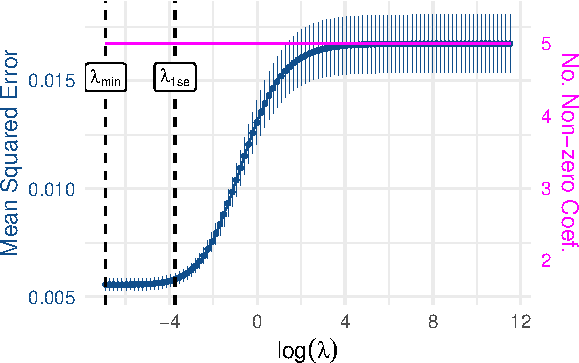
\includegraphics[keepaspectratio]{index_files/mediabag/regularisation_files/figure-pdf/fig-ridge-regression-1.pdf}}

}

\caption{\label{fig-ridge-regression}Cross-validation statistics for the
Ridge Regression approach applied to the seaweed data.}

\end{figure}%

Figure~\ref{fig-ridge-regression}, generated from the
\texttt{cv.glmnet()} object, illustrates the relationship between the
regularisation parameter \(\lambda\) and the model's cross-validation
performance. The \emph{y}-axis represents the mean squared error (MSE)
from cross-validation, whilst the \emph{x}-axis shows the
\(log(\lambda)\) values tested. Red dots indicate the mean MSE for each
\(\lambda\), with error bars showing ±1 standard error. Two vertical
dashed lines highlight important \(\lambda\) values: \(\lambda_{min}\),
which minimises the mean MSE, and \(\lambda_{1se}\), the largest
\(\lambda\) within one standard error of the minimum MSE. One may select
the optimal \(\lambda\) using either the \(\lambda_{min}\) or the
\(\lambda_{1se}\) rule, accessible via
\texttt{cv.glmnet\_object\$lambda.min} and
\texttt{cv.glmnet\_object\$lambda.1se}, respectively. To utilise the
chosen \(\lambda\), one refits the model using \texttt{glmnet()} and
extract the coefficients.

For performance evaluation, one can calculate the sum of squared
residuals (SSR) as the sum of squared differences between observed and
predicted values, and the R-squared value as the square of the
correlation between observed and predicted values, representing the
proportion of variance in the dependent variable that is predictable
from the independent variable(s).

The results show that the model explains 67.07\% of the variance in the
response variable:

\begin{Shaded}
\begin{Highlighting}[]
\CommentTok{\# Fit models and calculate performance metrics}
\NormalTok{fit\_model\_and\_calculate\_metrics }\OtherTok{\textless{}{-}} \ControlFlowTok{function}\NormalTok{(X, y, lambda) \{}
\NormalTok{  model }\OtherTok{\textless{}{-}} \FunctionTok{glmnet}\NormalTok{(X, y, }\AttributeTok{alpha =} \DecValTok{0}\NormalTok{, }\AttributeTok{lambda =}\NormalTok{ lambda,}
                  \AttributeTok{standardize =} \ConstantTok{TRUE}\NormalTok{)}
\NormalTok{  y\_hat }\OtherTok{\textless{}{-}} \FunctionTok{predict}\NormalTok{(model, X)}
\NormalTok{  ssr }\OtherTok{\textless{}{-}} \FunctionTok{sum}\NormalTok{((y }\SpecialCharTok{{-}}\NormalTok{ y\_hat) }\SpecialCharTok{\^{}} \DecValTok{2}\NormalTok{)}
\NormalTok{  rsq }\OtherTok{\textless{}{-}} \FunctionTok{cor}\NormalTok{(y, y\_hat) }\SpecialCharTok{\^{}} \DecValTok{2}
  \FunctionTok{list}\NormalTok{(}\AttributeTok{model =}\NormalTok{ model, }\AttributeTok{ssr =}\NormalTok{ ssr, }\AttributeTok{rsq =}\NormalTok{ rsq)}
\NormalTok{\}}

\CommentTok{\# Best cross{-}validated lambda}
\NormalTok{lambda\_cv }\OtherTok{\textless{}{-}}\NormalTok{ ridge\_cv}\SpecialCharTok{$}\NormalTok{lambda.min}
\NormalTok{mod\_cv }\OtherTok{\textless{}{-}} \FunctionTok{fit\_model\_and\_calculate\_metrics}\NormalTok{(X, y, lambda\_cv)}

\CommentTok{\# Print results}
\NormalTok{mod\_cv}
\SpecialCharTok{\textgreater{}} \ErrorTok{$}\NormalTok{model}
\SpecialCharTok{\textgreater{}} 
\ErrorTok{\textgreater{}}\NormalTok{ Call}\SpecialCharTok{:}  \FunctionTok{glmnet}\NormalTok{(}\AttributeTok{x =}\NormalTok{ X, }\AttributeTok{y =}\NormalTok{ y, }\AttributeTok{alpha =} \DecValTok{0}\NormalTok{, }\AttributeTok{lambda =}\NormalTok{ lambda, }\AttributeTok{standardize =} \ConstantTok{TRUE}\NormalTok{) }
\SpecialCharTok{\textgreater{}} 
\ErrorTok{\textgreater{}}\NormalTok{   Df  \%Dev Lambda}
\SpecialCharTok{\textgreater{}} \DecValTok{1}  \DecValTok{5} \FloatTok{67.06}  \FloatTok{0.001}
\SpecialCharTok{\textgreater{}} 
\ErrorTok{\textgreater{}} \ErrorTok{$}\NormalTok{ssr}
\SpecialCharTok{\textgreater{}}\NormalTok{ [}\DecValTok{1}\NormalTok{] }\FloatTok{5.321994}
\SpecialCharTok{\textgreater{}} 
\ErrorTok{\textgreater{}} \ErrorTok{$}\NormalTok{rsq}
\SpecialCharTok{\textgreater{}}\NormalTok{          s0}
\SpecialCharTok{\textgreater{}}\NormalTok{ Y }\FloatTok{0.6706681}
\end{Highlighting}
\end{Shaded}

As already indicated, an alternative to using \texttt{lambda.min} for
selecting the optimal \(\lambda\) value is to use the 1 SE rule, which
is contained in the attribute \texttt{lambda.1se}. This reduces the risk
of overfitting as it tends to select a simpler model. We can use this
value to refit the model and extract the coefficients, as before.

AIC and BIC can also be used to select suitable models. These
information criteria penalise the model for the number of parameters
used, providing a balance between model complexity and goodness of fit.
The \texttt{calculate\_ic()} function below calculates the AIC and BIC
for a given model and returns the results in a list. We can then use
this function to calculate the AIC and BIC for each model fit with each
\(\lambda\) in \texttt{lambdas\_to\_try}:

\begin{Shaded}
\begin{Highlighting}[]
\CommentTok{\# Calculate AIC and BIC}
\NormalTok{calculate\_ic }\OtherTok{\textless{}{-}} \ControlFlowTok{function}\NormalTok{(X, y, lambda) \{}
\NormalTok{  model }\OtherTok{\textless{}{-}} \FunctionTok{glmnet}\NormalTok{(X, y, }\AttributeTok{alpha =} \DecValTok{0}\NormalTok{, }\AttributeTok{lambda =}\NormalTok{ lambda,}
                  \AttributeTok{standardize =} \ConstantTok{TRUE}\NormalTok{)}
\NormalTok{  betas }\OtherTok{\textless{}{-}} \FunctionTok{as.vector}\NormalTok{(}\FunctionTok{coef}\NormalTok{(model)[}\SpecialCharTok{{-}}\DecValTok{1}\NormalTok{])}
\NormalTok{  resid }\OtherTok{\textless{}{-}}\NormalTok{ y }\SpecialCharTok{{-}}\NormalTok{ (}\FunctionTok{scale}\NormalTok{(X) }\SpecialCharTok{\%*\%}\NormalTok{ betas)}
\NormalTok{  H }\OtherTok{\textless{}{-}} \FunctionTok{scale}\NormalTok{(X) }\SpecialCharTok{\%*\%}
    \FunctionTok{solve}\NormalTok{(}\FunctionTok{t}\NormalTok{(}\FunctionTok{scale}\NormalTok{(X)) }\SpecialCharTok{\%*\%} \FunctionTok{scale}\NormalTok{(X) }\SpecialCharTok{+}\NormalTok{ lambda }\SpecialCharTok{*}
            \FunctionTok{diag}\NormalTok{(}\FunctionTok{ncol}\NormalTok{(X))) }\SpecialCharTok{\%*\%} \FunctionTok{t}\NormalTok{(}\FunctionTok{scale}\NormalTok{(X))}
\NormalTok{  df }\OtherTok{\textless{}{-}} \FunctionTok{sum}\NormalTok{(}\FunctionTok{diag}\NormalTok{(H))}
\NormalTok{  log\_resid\_ss }\OtherTok{\textless{}{-}} \FunctionTok{log}\NormalTok{(}\FunctionTok{sum}\NormalTok{(resid }\SpecialCharTok{\^{}} \DecValTok{2}\NormalTok{))}
\NormalTok{  aic }\OtherTok{\textless{}{-}} \FunctionTok{nrow}\NormalTok{(X) }\SpecialCharTok{*}\NormalTok{ log\_resid\_ss }\SpecialCharTok{+} \DecValTok{2} \SpecialCharTok{*}\NormalTok{ df}
\NormalTok{  bic }\OtherTok{\textless{}{-}} \FunctionTok{nrow}\NormalTok{(X) }\SpecialCharTok{*}\NormalTok{ log\_resid\_ss }\SpecialCharTok{+} \FunctionTok{log}\NormalTok{(}\FunctionTok{nrow}\NormalTok{(X)) }\SpecialCharTok{*}\NormalTok{ df}
  \FunctionTok{list}\NormalTok{(}\AttributeTok{aic =}\NormalTok{ aic, }\AttributeTok{bic =}\NormalTok{ bic)}
\NormalTok{\}}

\NormalTok{ic\_results }\OtherTok{\textless{}{-}} \FunctionTok{map}\NormalTok{(lambdas\_to\_try, }\SpecialCharTok{\textasciitilde{}} \FunctionTok{calculate\_ic}\NormalTok{(X, y, .x)) }\SpecialCharTok{|\textgreater{}}
  \FunctionTok{transpose}\NormalTok{()}
\end{Highlighting}
\end{Shaded}

A plot of the change in the information criteria with \(log(\lambda)\)
is shown in Figure~\ref{fig-aic-bic}. The optimal \(\lambda\) values
according to both AIC and BIC can then be used to refit the model and
arrive at the coefficients of interest.

\begin{Shaded}
\begin{Highlighting}[]
\CommentTok{\# Plot information criteria}
\NormalTok{plot\_ic }\OtherTok{\textless{}{-}} \ControlFlowTok{function}\NormalTok{(lambdas, ic\_results) \{}
\NormalTok{  df }\OtherTok{\textless{}{-}} \FunctionTok{data.frame}\NormalTok{(}\AttributeTok{lambda =} \FunctionTok{log}\NormalTok{(lambdas),}
                   \AttributeTok{aic =} \FunctionTok{unlist}\NormalTok{(ic\_results}\SpecialCharTok{$}\NormalTok{aic),}
                   \AttributeTok{bic =} \FunctionTok{unlist}\NormalTok{(ic\_results}\SpecialCharTok{$}\NormalTok{bic))}

\NormalTok{  df\_long }\OtherTok{\textless{}{-}} \FunctionTok{pivot\_longer}\NormalTok{(df, }\AttributeTok{cols =} \FunctionTok{c}\NormalTok{(aic, bic),}
                          \AttributeTok{names\_to =} \StringTok{"criterion"}\NormalTok{,}
                          \AttributeTok{values\_to =} \StringTok{"value"}\NormalTok{)}

  \FunctionTok{ggplot}\NormalTok{(df\_long, }\FunctionTok{aes}\NormalTok{(}\AttributeTok{x =}\NormalTok{ lambda, }\AttributeTok{y =}\NormalTok{ value, }\AttributeTok{color =}\NormalTok{ criterion)) }\SpecialCharTok{+}
    \FunctionTok{geom\_line}\NormalTok{() }\SpecialCharTok{+}
    \FunctionTok{scale\_color\_manual}\NormalTok{(}\AttributeTok{values =} \FunctionTok{c}\NormalTok{(}\StringTok{"aic"} \OtherTok{=} \StringTok{"orange"}\NormalTok{, }\StringTok{"bic"} \OtherTok{=} \StringTok{"skyblue3"}\NormalTok{),}
                       \AttributeTok{labels =} \FunctionTok{c}\NormalTok{(}\StringTok{"aic"} \OtherTok{=} \StringTok{"AIC"}\NormalTok{, }\StringTok{"bic"} \OtherTok{=} \StringTok{"BIC"}\NormalTok{)) }\SpecialCharTok{+}
    \FunctionTok{labs}\NormalTok{(}\AttributeTok{x =} \StringTok{"log(lambda)"}\NormalTok{,}
         \AttributeTok{y =} \StringTok{"Information Criterion"}\NormalTok{, }\AttributeTok{color =} \StringTok{"Criterion"}\NormalTok{) }\SpecialCharTok{+}
    \FunctionTok{theme\_minimal}\NormalTok{() }\SpecialCharTok{+}
    \FunctionTok{theme}\NormalTok{(}\AttributeTok{legend.position =} \StringTok{"top"}\NormalTok{,}
          \AttributeTok{legend.direction =} \StringTok{"horizontal"}\NormalTok{,}
          \AttributeTok{legend.box =} \StringTok{"horizontal"}\NormalTok{)}
\NormalTok{\}}

\FunctionTok{plot\_ic}\NormalTok{(lambdas\_to\_try, ic\_results)}
\end{Highlighting}
\end{Shaded}

\begin{figure}[tbp]

\centering{

\pandocbounded{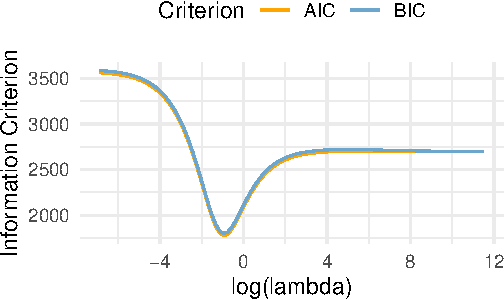
\includegraphics[keepaspectratio]{index_files/mediabag/regularisation_files/figure-pdf/fig-aic-bic-1.pdf}}

}

\caption{\label{fig-aic-bic}Plot of information criteria for best model
fit selected through Ridge Regression.}

\end{figure}%

Now we find the \(\lambda\) values that minimise the AIC and BIC, and
refit the models using these values. It so happens that both AIC and BIC
selects the same \(\lambda\) values:

\begin{Shaded}
\begin{Highlighting}[]
\CommentTok{\# Optimal lambdas according to both criteria}
\NormalTok{lambda\_aic }\OtherTok{\textless{}{-}}\NormalTok{ lambdas\_to\_try[}\FunctionTok{which.min}\NormalTok{(ic\_results}\SpecialCharTok{$}\NormalTok{aic)]}
\NormalTok{lambda\_bic }\OtherTok{\textless{}{-}}\NormalTok{ lambdas\_to\_try[}\FunctionTok{which.min}\NormalTok{(ic\_results}\SpecialCharTok{$}\NormalTok{bic)]}

\CommentTok{\# Fit final models using the optimal lambdas}
\NormalTok{mod\_aic }\OtherTok{\textless{}{-}} \FunctionTok{fit\_model\_and\_calculate\_metrics}\NormalTok{(X, y, lambda\_aic)}
\NormalTok{mod\_bic }\OtherTok{\textless{}{-}} \FunctionTok{fit\_model\_and\_calculate\_metrics}\NormalTok{(X, y, lambda\_bic)}
\end{Highlighting}
\end{Shaded}

For interest sake, we may also produce a plot that traces the
coefficients of the model as \(\lambda\) changes. This can help us
understand how the coefficients shrink as \(\lambda\) increases, and
which variables are most important in the model. The plot below shows
the Ridge Regression coefficients path for each variable in the model
(Figure~\ref{fig-coef-path1}).

\begin{Shaded}
\begin{Highlighting}[]
\CommentTok{\# Plot the Ridge Regression coefficients path}
\NormalTok{res }\OtherTok{\textless{}{-}} \FunctionTok{glmnet}\NormalTok{(X, y, }\AttributeTok{alpha =} \DecValTok{0}\NormalTok{, }\AttributeTok{lambda =}\NormalTok{ lambdas\_to\_try,}
              \AttributeTok{standardize =} \ConstantTok{FALSE}\NormalTok{)}
\FunctionTok{plot}\NormalTok{(res, }\AttributeTok{xvar =} \StringTok{"lambda"}\NormalTok{)}
\FunctionTok{legend}\NormalTok{(}\StringTok{"topright"}\NormalTok{, }\AttributeTok{lwd =} \DecValTok{1}\NormalTok{, }\AttributeTok{col =} \DecValTok{1}\SpecialCharTok{:}\DecValTok{6}\NormalTok{,}
       \AttributeTok{legend =} \FunctionTok{colnames}\NormalTok{(X), }\AttributeTok{cex =} \FloatTok{0.7}\NormalTok{)}
\end{Highlighting}
\end{Shaded}

\begin{figure}[tbp]

\centering{

\pandocbounded{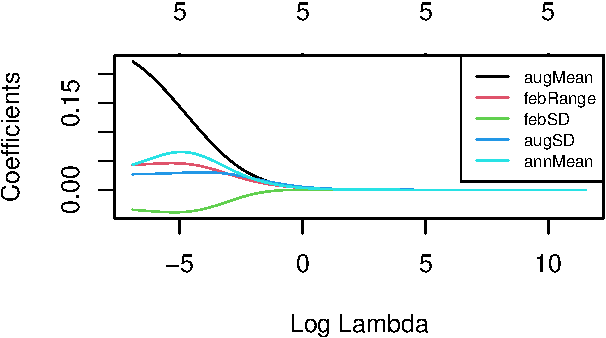
\includegraphics[keepaspectratio]{index_files/mediabag/regularisation_files/figure-pdf/fig-coef-path1-1.pdf}}

}

\caption{\label{fig-coef-path1}Plot of the Ridge Regression coefficients
paths.}

\end{figure}%

So, after having demonstrated the different methods for selecting the
optimal \(\lambda\) value, we can now summarise the results:

\begin{verbatim}
> [1] "CV Lambda: 0.001"
> [1] "AIC Lambda: 0.3854"
> [1] "BIC Lambda: 0.3854"
> [1] "CV R-squared: 0.6707"
> [1] "AIC R-squared: 0.6025"
> [1] "BIC R-squared: 0.6025"
\end{verbatim}

Now we can extract the coefficient produced from models selected via the
AIC and CV methods.

\begin{Shaded}
\begin{Highlighting}[]
\NormalTok{res\_aic }\OtherTok{\textless{}{-}} \FunctionTok{glmnet}\NormalTok{(X, y, }\AttributeTok{alpha =} \DecValTok{0}\NormalTok{, }\AttributeTok{lambda =}\NormalTok{ lambda\_aic,}
                  \AttributeTok{standardize =} \ConstantTok{FALSE}\NormalTok{)}
\NormalTok{res\_aic}
\SpecialCharTok{\textgreater{}} 
\ErrorTok{\textgreater{}}\NormalTok{ Call}\SpecialCharTok{:}  \FunctionTok{glmnet}\NormalTok{(}\AttributeTok{x =}\NormalTok{ X, }\AttributeTok{y =}\NormalTok{ y, }\AttributeTok{alpha =} \DecValTok{0}\NormalTok{, }\AttributeTok{lambda =}\NormalTok{ lambda\_aic, }\AttributeTok{standardize =} \ConstantTok{FALSE}\NormalTok{) }
\SpecialCharTok{\textgreater{}} 
\ErrorTok{\textgreater{}}\NormalTok{   Df  \%Dev Lambda}
\SpecialCharTok{\textgreater{}} \DecValTok{1}  \DecValTok{5} \FloatTok{13.46} \FloatTok{0.3854}
\FunctionTok{coef}\NormalTok{(res\_aic)}
\SpecialCharTok{\textgreater{}} \DecValTok{6}\NormalTok{ x }\DecValTok{1}\NormalTok{ sparse Matrix of class }\StringTok{"dgCMatrix"}
\SpecialCharTok{\textgreater{}}\NormalTok{                       s0}
\SpecialCharTok{\textgreater{}}\NormalTok{ (Intercept) }\SpecialCharTok{{-}}\FloatTok{0.021327121}
\SpecialCharTok{\textgreater{}}\NormalTok{ augMean      }\FloatTok{0.009856026}
\SpecialCharTok{\textgreater{}}\NormalTok{ febRange     }\FloatTok{0.007118466}
\SpecialCharTok{\textgreater{}}\NormalTok{ febSD       }\SpecialCharTok{{-}}\FloatTok{0.001074341}
\SpecialCharTok{\textgreater{}}\NormalTok{ augSD        }\FloatTok{0.010696102}
\SpecialCharTok{\textgreater{}}\NormalTok{ annMean      }\FloatTok{0.008114467}
\end{Highlighting}
\end{Shaded}

\begin{Shaded}
\begin{Highlighting}[]
\NormalTok{res\_cv }\OtherTok{\textless{}{-}} \FunctionTok{glmnet}\NormalTok{(X, y, }\AttributeTok{alpha =} \DecValTok{0}\NormalTok{, }\AttributeTok{lambda =}\NormalTok{ lambda\_cv,}
                 \AttributeTok{standardize =} \ConstantTok{FALSE}\NormalTok{)}
\NormalTok{res\_cv}
\SpecialCharTok{\textgreater{}} 
\ErrorTok{\textgreater{}}\NormalTok{ Call}\SpecialCharTok{:}  \FunctionTok{glmnet}\NormalTok{(}\AttributeTok{x =}\NormalTok{ X, }\AttributeTok{y =}\NormalTok{ y, }\AttributeTok{alpha =} \DecValTok{0}\NormalTok{, }\AttributeTok{lambda =}\NormalTok{ lambda\_cv, }\AttributeTok{standardize =} \ConstantTok{FALSE}\NormalTok{) }
\SpecialCharTok{\textgreater{}} 
\ErrorTok{\textgreater{}}\NormalTok{   Df  \%Dev Lambda}
\SpecialCharTok{\textgreater{}} \DecValTok{1}  \DecValTok{5} \FloatTok{66.77}  \FloatTok{0.001}
\FunctionTok{coef}\NormalTok{(res\_cv)}
\SpecialCharTok{\textgreater{}} \DecValTok{6}\NormalTok{ x }\DecValTok{1}\NormalTok{ sparse Matrix of class }\StringTok{"dgCMatrix"}
\SpecialCharTok{\textgreater{}}\NormalTok{                      s0}
\SpecialCharTok{\textgreater{}}\NormalTok{ (Intercept) }\SpecialCharTok{{-}}\FloatTok{0.12384440}
\SpecialCharTok{\textgreater{}}\NormalTok{ augMean      }\FloatTok{0.22200994}
\SpecialCharTok{\textgreater{}}\NormalTok{ febRange     }\FloatTok{0.04287655}
\SpecialCharTok{\textgreater{}}\NormalTok{ febSD       }\SpecialCharTok{{-}}\FloatTok{0.03446642}
\SpecialCharTok{\textgreater{}}\NormalTok{ augSD        }\FloatTok{0.02699458}
\SpecialCharTok{\textgreater{}}\NormalTok{ annMean      }\FloatTok{0.04324177}
\end{Highlighting}
\end{Shaded}

Ridge regression adds a penalty to the size of the coefficients,
resulting in their shrinkage towards zero. This penalty affects all
coefficients simultaneously. Notably, there is a difference in the model
fit obtained using \(\lambda_{AIC}\) (which is larger) and
\(\lambda_{min}\) (which is smaller). The former model explains 55.69\%
of the variance, compared to \(\lambda_{min}\), which explains 63.37\%
of the variance.

Although shrinkage affects the absolute magnitude of the coefficients
(they are biased estimates of the true relationships between the
predictors and the response variable), the coefficients in Ridge
Regression retain their general meaning---they still represent the
change in the response variable associated with a one-unit change in the
predictor variable, holding other predictors constant. While the
absolute values of the coefficients may be biased due to regularisation,
the relative importance of the predictors can still be interpreted. The
magnitude of the coefficients can indicate the relative influence of
each predictor on the response variable, even if their exact values are
reduced.

Importantly, the predictive ability of the model can improve with shrunk
coefficients because Ridge Regression reduces overfitting and enhances
the model's generalisability to new, unseen data. By stabilising the
coefficient estimates, the model often achieves better performance on
validation and test datasets, which is important should robust
predictive analytics be the goal.

\section{Example 2: Lasso Regression}\label{example-2-lasso-regression}

Doing a Lasso Regression is easy. Simply change the \texttt{alpha}
parameter to 1 in the \texttt{glmnet} function. The rest of the code
remains the same. I'll show only the final output of this analysis to
avoid repetition.

\begin{Shaded}
\begin{Highlighting}[]
\CommentTok{\# Print results}
\NormalTok{mod\_cv}
\SpecialCharTok{\textgreater{}} \ErrorTok{$}\NormalTok{model}
\SpecialCharTok{\textgreater{}} 
\ErrorTok{\textgreater{}}\NormalTok{ Call}\SpecialCharTok{:}  \FunctionTok{glmnet}\NormalTok{(}\AttributeTok{x =}\NormalTok{ X, }\AttributeTok{y =}\NormalTok{ y, }\AttributeTok{alpha =} \DecValTok{1}\NormalTok{, }\AttributeTok{lambda =}\NormalTok{ lambda, }\AttributeTok{standardize =} \ConstantTok{TRUE}\NormalTok{) }
\SpecialCharTok{\textgreater{}} 
\ErrorTok{\textgreater{}}\NormalTok{   Df \%Dev Lambda}
\SpecialCharTok{\textgreater{}} \DecValTok{1}  \DecValTok{5}   \DecValTok{67}  \FloatTok{0.001}
\SpecialCharTok{\textgreater{}} 
\ErrorTok{\textgreater{}} \ErrorTok{$}\NormalTok{ssr}
\SpecialCharTok{\textgreater{}}\NormalTok{ [}\DecValTok{1}\NormalTok{] }\FloatTok{5.332835}
\SpecialCharTok{\textgreater{}} 
\ErrorTok{\textgreater{}} \ErrorTok{$}\NormalTok{rsq}
\SpecialCharTok{\textgreater{}}\NormalTok{          s0}
\SpecialCharTok{\textgreater{}}\NormalTok{ Y }\FloatTok{0.6701255}
\FunctionTok{coef}\NormalTok{(mod\_cv}\SpecialCharTok{$}\NormalTok{model)}
\SpecialCharTok{\textgreater{}} \DecValTok{6}\NormalTok{ x }\DecValTok{1}\NormalTok{ sparse Matrix of class }\StringTok{"dgCMatrix"}
\SpecialCharTok{\textgreater{}}\NormalTok{                      s0}
\SpecialCharTok{\textgreater{}}\NormalTok{ (Intercept) }\SpecialCharTok{{-}}\FloatTok{0.12886019}
\SpecialCharTok{\textgreater{}}\NormalTok{ augMean      }\FloatTok{0.26097296}
\SpecialCharTok{\textgreater{}}\NormalTok{ febRange     }\FloatTok{0.03431981}
\SpecialCharTok{\textgreater{}}\NormalTok{ febSD       }\SpecialCharTok{{-}}\FloatTok{0.02497532}
\SpecialCharTok{\textgreater{}}\NormalTok{ augSD        }\FloatTok{0.02441380}
\SpecialCharTok{\textgreater{}}\NormalTok{ annMean      }\FloatTok{0.02021480}

\CommentTok{\# Print results}
\FunctionTok{print}\NormalTok{(}\FunctionTok{paste}\NormalTok{(}\StringTok{"CV Lambda:"}\NormalTok{, lambda\_cv))}
\SpecialCharTok{\textgreater{}}\NormalTok{ [}\DecValTok{1}\NormalTok{] }\StringTok{"CV Lambda: 0.001"}
\FunctionTok{print}\NormalTok{(}\FunctionTok{paste}\NormalTok{(}\StringTok{"CV R{-}squared:"}\NormalTok{, }\FunctionTok{round}\NormalTok{(mod\_cv}\SpecialCharTok{$}\NormalTok{rsq, }\DecValTok{4}\NormalTok{)))}
\SpecialCharTok{\textgreater{}}\NormalTok{ [}\DecValTok{1}\NormalTok{] }\StringTok{"CV R{-}squared: 0.6701"}
\end{Highlighting}
\end{Shaded}

\begin{figure}[tbp]

\centering{

\pandocbounded{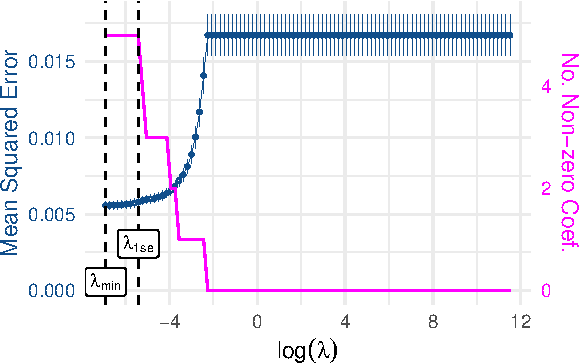
\includegraphics[keepaspectratio]{index_files/mediabag/regularisation_files/figure-pdf/fig-lasso-regression-1.pdf}}

}

\caption{\label{fig-lasso-regression}Cross-validation statistics for
Lasso Regression applied to the seaweed data.}

\end{figure}%

\begin{figure}[tbp]

\centering{

\pandocbounded{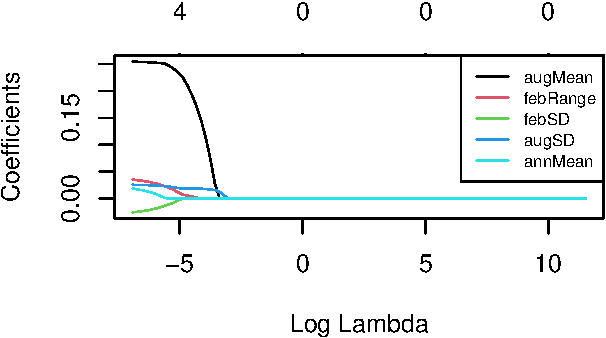
\includegraphics[keepaspectratio]{index_files/mediabag/regularisation_files/figure-pdf/fig-coef-path2-1.pdf}}

}

\caption{\label{fig-coef-path2}Plot of the Lasso Regression coefficients
paths.}

\end{figure}%

Lasso regression incorporates an L1 penalty term in its cost function,
which shrinks some coefficient estimates to exactly zero. By reducing
certain coefficients to zero, Lasso effectively eliminates those
predictors from the model, which achieves automatic variable selection:

\begin{itemize}
\tightlist
\item
  When \(\lambda\) is small, the penalty is minimal, and Lasso behaves
  similarly to ordinary least squares regression, retaining most
  coefficients.
\item
  When \(\lambda\) is large, the penalty increases, causing more
  coefficients to shrink to zero. This results in a sparser model where
  only the most significant predictors have non-zero coefficients.
\end{itemize}

In our example (Figure~\ref{fig-lasso-regression}), we see at
\(\lambda_{min}\), the number of non-zero coefficients is
minimised---all five coefficients remain. At \(\lambda_{1se}\), the
number of non-zero coefficients decreases to four. Consequently, for
higher values of \(\lambda\), more predictors will have coefficients
exactly equal to zero. This is also seen in
Figure~\ref{fig-lasso-regression}. In Figure~\ref{fig-coef-path2} we can
see that the first predictor to reach zero is \texttt{annMean}, then
\texttt{febSD}, \texttt{febRange}, and so forth. The implication is that
they are excluded from the model and the model is simplified. This leads
to several benefits: reduced multicollinearity, improved
interpretability, and better generalisation to new data.

Coefficients that remain non-zero after Lasso regularisation are
considered more important predictors. Those remaining coefficients can
be interpreted similarly to standard linear regression: as the expected
change in the response variable for a one-unit change in the predictor,
holding other predictors constant.

The \(\lambda\) parameter controls the amount of bias introduced. While
Lasso can produce biased estimates, it reduces variance, often resulting
in a model that performs better on new, unseen data. This trade-off
enhances predictive accuracy but means that the exact coefficient values
may not represent the true underlying relationships as closely as those
in an unregularised model.

Despite regularisation, the relative magnitudes of the non-zero
coefficients provide a glimpse into predictor importance. Larger
absolute values of coefficients indicate stronger relationships with the
response variable. The exact numerical values are biased, but ranking
predictors by their coefficients still offers useful insight into their
relative importance.

\section{Example 3: Elastic Net
Regression}\label{example-3-elastic-net-regression}

In this last example we'll look at Elastic Net Regression, which
combines the L1 and L2 penalties of Lasso and Ridge Regression. There
are now two parameters to optimise: \(\alpha\) and \(\lambda\). The
\(\alpha\) parameter controls the mix between the L1 and L2 penalties,
with \(\alpha = 0\) behaving like Ridge Regression and \(\alpha = 1\)
behaving like Lasso Regression. For \(\alpha\) values between 0 and 1,
Elastic Net combines the strengths of both Lasso and Ridge Regression.
Optimisation of \(\alpha\) and \(\lambda\) is also done using
cross-validation. In practise, the steps are:

\begin{enumerate}
\def\labelenumi{\arabic{enumi}.}
\tightlist
\item
  Set up a grid of \(\alpha\) values (from 0 to 1) and \(\lambda\)
  values to try.
\item
  Performs cross-validation for each combination of \(\alpha\) and
  \(\lambda\) using \texttt{cv.glmnet()}.
\item
  Select the best \(\alpha\) and \(\lambda\) combination based on the
  minimum mean cross-validated error.
\item
  Fit the final model using the best \(\alpha\) and \(\lambda\).
\item
  Calculate the performance metrics.
\item
  For the Elastic Net model with the best alphaCreate plots similar to
  those in the Ridge and Lasso examples.
\end{enumerate}

\begin{Shaded}
\begin{Highlighting}[]
\CommentTok{\# Define the range of alpha values to try}
\NormalTok{alphas\_to\_try }\OtherTok{\textless{}{-}} \FunctionTok{seq}\NormalTok{(}\DecValTok{0}\NormalTok{, }\DecValTok{1}\NormalTok{, }\AttributeTok{by =} \FloatTok{0.1}\NormalTok{)}

\CommentTok{\# Define the range of lambda values to try}
\NormalTok{lambdas\_to\_try }\OtherTok{\textless{}{-}} \DecValTok{10}\SpecialCharTok{\^{}}\FunctionTok{seq}\NormalTok{(}\SpecialCharTok{{-}}\DecValTok{3}\NormalTok{, }\DecValTok{3}\NormalTok{, }\AttributeTok{length.out =} \DecValTok{100}\NormalTok{)}

\CommentTok{\# Perform grid search with cross{-}validation}
\NormalTok{cv\_results }\OtherTok{\textless{}{-}} \FunctionTok{lapply}\NormalTok{(alphas\_to\_try, }\ControlFlowTok{function}\NormalTok{(a) \{}
  \FunctionTok{cv.glmnet}\NormalTok{(X, y, }\AttributeTok{alpha =}\NormalTok{ a, }\AttributeTok{lambda =}\NormalTok{ lambdas\_to\_try,}
            \AttributeTok{standardize =} \ConstantTok{TRUE}\NormalTok{, }\AttributeTok{nfolds =} \DecValTok{10}\NormalTok{)}
\NormalTok{\})}

\CommentTok{\# Find the best alpha and lambda}
\NormalTok{best\_result }\OtherTok{\textless{}{-}} \FunctionTok{which.min}\NormalTok{(}\FunctionTok{sapply}\NormalTok{(cv\_results, }\ControlFlowTok{function}\NormalTok{(x) }\FunctionTok{min}\NormalTok{(x}\SpecialCharTok{$}\NormalTok{cvm)))}
\NormalTok{best\_alpha }\OtherTok{\textless{}{-}}\NormalTok{ alphas\_to\_try[best\_result]}
\NormalTok{best\_lambda }\OtherTok{\textless{}{-}}\NormalTok{ cv\_results[[best\_result]]}\SpecialCharTok{$}\NormalTok{lambda.min}

\CommentTok{\# Fit the final model with the best parameters}
\NormalTok{final\_model }\OtherTok{\textless{}{-}} \FunctionTok{glmnet}\NormalTok{(X, y, }\AttributeTok{alpha =}\NormalTok{ best\_alpha,}
                      \AttributeTok{lambda =}\NormalTok{ best\_lambda,}
                      \AttributeTok{standardize =} \ConstantTok{TRUE}\NormalTok{)}

\CommentTok{\# Calculate performance metrics}
\NormalTok{y\_hat }\OtherTok{\textless{}{-}} \FunctionTok{predict}\NormalTok{(final\_model, X)}
\NormalTok{ssr }\OtherTok{\textless{}{-}} \FunctionTok{sum}\NormalTok{((y }\SpecialCharTok{{-}}\NormalTok{ y\_hat) }\SpecialCharTok{\^{}} \DecValTok{2}\NormalTok{)}
\NormalTok{rsq }\OtherTok{\textless{}{-}} \FunctionTok{cor}\NormalTok{(y, y\_hat) }\SpecialCharTok{\^{}} \DecValTok{2}
\end{Highlighting}
\end{Shaded}

\begin{verbatim}
> [1] "Best Alpha: 0.3"
> [1] "Best Lambda: 0.001"
> [1] "R-squared: 0.6706"
\end{verbatim}

\begin{figure}[tbp]

\centering{

\pandocbounded{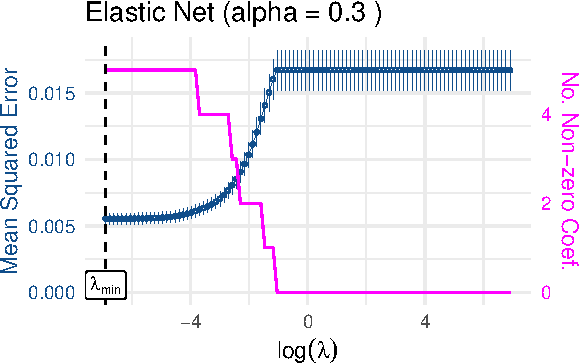
\includegraphics[keepaspectratio]{index_files/mediabag/regularisation_files/figure-pdf/fig-elastic-net-regression-1.pdf}}

}

\caption{\label{fig-elastic-net-regression}Cross-validation statistics
for Elastic Net Regression applied to the seaweed data.}

\end{figure}%

\begin{figure}[tbp]

\centering{

\pandocbounded{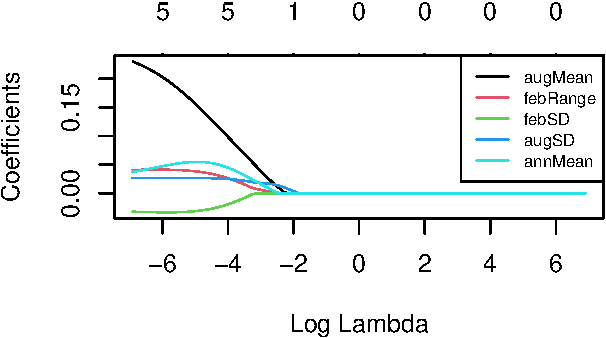
\includegraphics[keepaspectratio]{index_files/mediabag/regularisation_files/figure-pdf/fig-coef-path3-1.pdf}}

}

\caption{\label{fig-coef-path3}Plot of the Elastic Net Regression
coefficients paths.}

\end{figure}%

The model coefficients are:

\begin{Shaded}
\begin{Highlighting}[]
\FunctionTok{coef}\NormalTok{(cv\_results[[best\_result]])}
\SpecialCharTok{\textgreater{}} \DecValTok{6}\NormalTok{ x }\DecValTok{1}\NormalTok{ sparse Matrix of class }\StringTok{"dgCMatrix"}
\SpecialCharTok{\textgreater{}}\NormalTok{                       s1}
\SpecialCharTok{\textgreater{}}\NormalTok{ (Intercept) }\SpecialCharTok{{-}}\FloatTok{0.117063010}
\SpecialCharTok{\textgreater{}}\NormalTok{ augMean      }\FloatTok{0.240447330}
\SpecialCharTok{\textgreater{}}\NormalTok{ febRange     }\FloatTok{0.015404286}
\SpecialCharTok{\textgreater{}}\NormalTok{ febSD       }\SpecialCharTok{{-}}\FloatTok{0.007224065}
\SpecialCharTok{\textgreater{}}\NormalTok{ augSD        }\FloatTok{0.014882111}
\SpecialCharTok{\textgreater{}}\NormalTok{ annMean      }\FloatTok{0.026504736}
\end{Highlighting}
\end{Shaded}

The interpretation of coefficients in Elastic Net is a blend of Ridge
and Lasso. Some coefficients may be shrunk to zero (feature selection),
while others are shrunk but remain non-zero (magnitude reduction). The
non-zero coefficients retain their general meaning with an emphasis on
their relative importance.

\section{Theory-Driven and Data-Driven Variable
Selection}\label{theory-driven-and-data-driven-variable-selection}

The choice between theory-driven and data- or statistics-driven variable
selection represents an important consideration that can greatly
influence model interpretation, its predictive power, and your value as
an ecologist. This decision reflects a broader tension in scientific
methodology between deductive and inductive reasoning. Each offers
advantages and limitations that you should be aware of as an ecologist.

Theory-driven variable selection is core to the scientific method. It
relies on \emph{a priori} knowledge and established ecological theories
(as far as they exist in ecology!) to guide your choice of predictors in
a model. This aligns closely with the hypothetico-deductive method,
where we formulate hypotheses based on existing knowledge and
subsequently test these against the data we collect. The strength of
this method lies in its interpretability. Models built on theoretical
foundations often contribute directly to testing and refining ecological
hypotheses. By focusing on variables with known or hypothesised
relationships (with mechanisms often rooted in ecophysiological or
ecological inquiries), the theory-driven hypothetico-deductive method
should lead to more parsimonious models that are less prone to
overfitting and more reflecting of reality.

Theory-driven selection is not without its drawbacks. It requires that
we have a good grasp of the mechanism underlying our favourite
ecological system. This is not always the case in complex systems where
the underlying mechanisms are not well understood. Theory-driven
selection can then lead to the exclusion of important variables that
were not initially hypothesised and it can limit the scope of the
analysis and potentially overlook significant relationships in the data.

A naive young ecologist might place undue value on the notion that their
hard work collecting diverse data and developing hypotheses should all
be reflected in their final model. This can lead to confirmation bias,
where one is more likely to select variables that support our hypotheses
and ignore those that do not. This bias can compromise the objectivity
of the model and lead to skewed results that do not accurately represent
the underlying ecological processes.

Moreover, the insistence on including all variables that were initially
considered important can result in overly complex models. Such models
can be difficult to interpret and may suffer from overfitting, where the
model captures noise rather than the true signal in the data. Overfitted
models perform well on the data we collected but poorly on new, unseen
data. The consequence is a loss of predictive power and
generalisability.

Another weakness of theory-driven variable selection is that the
reliance on existing theories or the novel, promising hypothsis of the
day may lead us to overlook important but unexpected relationships in
the data. In complex ecological systems, where our theoretical
understanding may be incomplete, some variables could be missed
entirely---these might in fact hold the key to the real cause of the
ecological patterns we observe. This limitation becomes concerning when
studying ecosystems or phenomena that are not well understood or are
undergoing rapid changes, such as those affected by climate change or
novel anthropogenic pressures.

On the other hand, data-driven approaches, including regularisation
techniques, VIF, and forward model variable selection
(Chapter~\ref{sec-multiple-linear-regression}), allow the data itself to
guide variable selection. These methods are increasingly used in today's
era of high-dimensional datasets common in modern ecological research.
The primary advantage of data-driven selection lies in its potential for
discovery---it can uncover unexpected relationships and generate new
hypotheses, which is valuable in complex ecological systems where
interactions may not be immediately apparent.

Data-driven methods are well-suited for handling the complexity often
encountered in environmental and ecological datasets, where numerous
potential predictors may co-occur and interact. They offer a degree of
objectivity, reducing the potential for our personal biases in variable
selection. But these approaches are not without risks. There's a danger
of identifying relationships that are statistically significant but
ecologically meaningless---we refer to this as spurious correlations
(e.g.~the belief that consuming carrots significantly improves our night
vision). Moreover, models with many variables can present significant
interpretability challenges, especially when complex interactions are
present. This can make it difficult to extract meaningful (plausible)
insights from the model and to communicate results to a broader
audience.

In practice, the most robust approach to selecting which of the
multitude of variables to include in our model often involves a
thoughtful combination of theory-driven and data-driven methods.
Well-trained ecologists should start with theory-driven variable
selection to identify the core predictors based on established
ecological principles. We could then employ regularisation techniques to
explore additional variables and potential interactions, and use the
results to refine our models and generate new hypotheses for future
research.

This hybrid approach combines the strengths of both methods. It allows
for rigorous hypothesis testing while remaining open to unanticipated
and new insights from the data. In ecology, where systems are often
characterised by complex, non-linear relationships and interactions that
may vary across spatial and temporal scales, this two-pronged approach
offers distinct benefits.

Consider how these methods complement theoretical knowledge. Use
variable selection methods as tools for prediction, and to assit
generating new insights and hypotheses about ecosystems. The choice
between theory-driven and data-driven variable selection is not a binary
one, but rather a spectrum of approaches.

\part{Regression Analysis}

\chapter{Testing Assumptions}\label{sec-assumption-tests}

Assumption tests are a fundamental component of any statistical analysis
workflow. They ensure the validity, reliability, and robustness of
statistical analyses. Although these tests test assumptions about
parametric statistical methods, they are generally non-parametric,
meaning they do not assume a specific probability distribution for the
data.

\section{Tests for Normality}\label{tests-for-normality}

In biological research, it is often important to determine whether a
normal distribution adequately represents the underlying population
distribution. This assessment is relevant when applying statistical
procedures that rely on the assumption of normality, such as many of
those discussed in earlier chapters. However, note that not all
biological data conform to a normal distribution. In fact, many natural
processes will result in non-normal data.

Assessing normality allows us to make informed decisions about
appropriate statistical methods. If the data reasonably approximates a
normal distribution, we can confidently apply parametric tests using
probability calculations based on the normal curve. Conversely, if the
data significantly deviates from normality, alternative non-parametric
approaches may be more suitable.

Beyond simply validating statistical assumptions, examining the
distribution of biological data can offer valuable insights into the
underlying mechanisms and processes shaping the population. Identifying
deviations from normality can challenge existing hypotheses, reveal
hidden patterns, or suggest the influence of unanticipated factors.
Therefore, normality tests are not only a technical requirement but they
may also offer a tool for understanding the biological phenomena under
investigation.

In this section, we will explore a range of graphical methods (e.g.,
histograms, Q-Q plots) and statistical tests (e.g., Shapiro-Wilk test,
Kolmogorov-Smirnov test) to assess the goodness-of-fit of a normal
distribution to our data.

\subsection{Shapiro-Wilk Test}\label{shapiro-wilk-test}

\subsection{Kolmogorov-Smirnov Test}\label{kolmogorov-smirnov-test}

\subsection{Anderson-Darling Test}\label{anderson-darling-test}

\subsection{Lilliefors Test}\label{lilliefors-test}

\subsection{Jarque-Bera Test}\label{jarque-bera-test}

\section{Tests for Homoscedasticity}\label{tests-for-homoscedasticity}

\subsection{Breusch-Pagan Test}\label{breusch-pagan-test}

\subsection{White's Test}\label{whites-test}

\subsection{Levene's Test}\label{levenes-test}

\subsection{Bartlett's Test}\label{bartletts-test}

\subsection{Fligner-Killeen Test}\label{fligner-killeen-test}

\chapter{Quantile Regression}\label{quantile-regression}

In traditional quantile regression, we model the conditional quantiles
of the response variable given the predictor variables. However, when
you want to study how different quantiles of the predictor variable
(e.g., wind stress curl) affect the response variable (e.g., SST and
upwelling metrics), you need to employ methods that can capture these
dynamics.

\section{Understanding the Challenge}\label{understanding-the-challenge}

\begin{itemize}
\tightlist
\item
  \textbf{Standard Quantile Regression:} Models the relationship between
  predictor variables and specific quantiles of the response variable.
\item
  \textbf{Your Objective:} To understand how different quantiles of the
  predictor variable influence the response variable.
\end{itemize}

\section{Possible Approaches}\label{possible-approaches}

\begin{enumerate}
\def\labelenumi{\arabic{enumi}.}
\item
  \textbf{Quantile-on-Quantile Regression (QQR):}

  \begin{itemize}
  \tightlist
  \item
    \textbf{Concept:}

    \begin{itemize}
    \tightlist
    \item
      QQR extends traditional quantile regression by examining how
      quantiles of the predictor variable affect quantiles of the
      response variable.
    \item
      It provides a more comprehensive picture of the dependence
      structure between the two variables across their entire
      distributions.
    \end{itemize}
  \item
    \textbf{Implementation Steps:}

    \begin{enumerate}
    \def\labelenumii{\arabic{enumii}.}
    \tightlist
    \item
      \textbf{Estimate Conditional Quantiles of the Predictor Variable:}

      \begin{itemize}
      \tightlist
      \item
        For each quantile \(\tau\) of the predictor variable (wind
        stress curl), calculate the quantile values.
      \end{itemize}
    \item
      \textbf{Model Response Quantiles Conditional on Predictor
      Quantiles:}

      \begin{itemize}
      \tightlist
      \item
        For each quantile \(\theta\) of the response variable (SST),
        model it as a function of the predictor variable's quantiles.
      \item
        The model can be specified as:
        \[Q_{\theta}(SST \mid Q_{\tau}(\text{Wind Stress Curl})) = \beta_0(\theta, \tau) + \beta_1(\theta, \tau) \times Q_{\tau}(\text{Wind Stress Curl})\]
      \end{itemize}
    \item
      \textbf{Interpretation:}

      \begin{itemize}
      \tightlist
      \item
        The coefficients \(\beta_1(\theta, \tau)\) show how the
        \(\tau\)-th quantile of the wind stress curl affects the
        \(\theta\)-th quantile of SST.
      \item
        By varying \(\theta\) and \(\tau\), you can map out the entire
        dependence structure.
      \end{itemize}
    \end{enumerate}
  \item
    \textbf{Advantages:}

    \begin{itemize}
    \tightlist
    \item
      Captures non-linear and asymmetric relationships between the
      variables.
    \item
      Allows for interactions between different parts of the
      distributions.
    \end{itemize}
  \item
    \textbf{Considerations:}

    \begin{itemize}
    \tightlist
    \item
      \textbf{Computational Complexity:} Estimating the model for all
      combinations of \(\theta\) and \(\tau\) can be computationally
      intensive.
    \item
      \textbf{Data Requirements:} Requires a large dataset to obtain
      reliable estimates across quantiles.
    \end{itemize}
  \end{itemize}
\item
  \textbf{Binning the Predictor Variable:}

  \begin{itemize}
  \tightlist
  \item
    \textbf{Concept:}

    \begin{itemize}
    \tightlist
    \item
      Divide the predictor variable into bins based on its quantiles
      (e.g., quartiles or deciles).
    \item
      Within each bin, analyse the relationship between the predictor
      and response variable.
    \end{itemize}
  \item
    \textbf{Implementation Steps:}

    \begin{enumerate}
    \def\labelenumii{\arabic{enumii}.}
    \tightlist
    \item
      \textbf{Quantile Binning:}

      \begin{itemize}
      \tightlist
      \item
        Divide wind stress curl data into quantile-based bins.
      \end{itemize}
    \item
      \textbf{Within-Bin Analysis:}

      \begin{itemize}
      \tightlist
      \item
        For each bin, perform regression analysis to see how variations
        within that bin affect SST.
      \end{itemize}
    \item
      \textbf{Comparative Analysis:}

      \begin{itemize}
      \tightlist
      \item
        Compare the regression coefficients across bins to see if the
        effect of wind stress curl on SST changes across its
        distribution.
      \end{itemize}
    \end{enumerate}
  \item
    \textbf{Advantages:}

    \begin{itemize}
    \tightlist
    \item
      Simpler to implement and interpret.
    \item
      Highlights non-linear relationships and threshold effects.
    \end{itemize}
  \item
    \textbf{Considerations:}

    \begin{itemize}
    \tightlist
    \item
      \textbf{Loss of Information:} Binning can lead to loss of
      information due to grouping continuous data.
    \item
      \textbf{Boundary Issues:} Care must be taken at the edges of bins
      to ensure continuity.
    \end{itemize}
  \end{itemize}
\item
  \textbf{Interaction Terms and Non-Linear Models:}

  \begin{itemize}
  \tightlist
  \item
    \textbf{Concept:}

    \begin{itemize}
    \tightlist
    \item
      Introduce interaction terms or non-linear transformations to allow
      the effect of wind stress curl to vary across its own
      distribution.
    \end{itemize}
  \item
    \textbf{Implementation Steps:}

    \begin{enumerate}
    \def\labelenumii{\arabic{enumii}.}
    \tightlist
    \item
      \textbf{Create Interaction Terms:}

      \begin{itemize}
      \tightlist
      \item
        Include terms like
        \(\text{Wind Stress Curl} \times I(\text{Wind Stress Curl} > Q_{\tau})\),
        where \(I\) is an indicator function, and \(Q_{\tau}\) is the
        \(\tau\)-th quantile.
      \end{itemize}
    \item
      \textbf{Non-Linear Models:}

      \begin{itemize}
      \tightlist
      \item
        Use models like Generalised Additive Models (GAMs) to allow for
        non-linear relationships.
      \end{itemize}
    \item
      \textbf{Quantile Regression with Interactions:}

      \begin{itemize}
      \tightlist
      \item
        Combine quantile regression with interaction terms to see how
        the effect changes at different levels of the predictor
        variable.
      \end{itemize}
    \end{enumerate}
  \item
    \textbf{Advantages:}

    \begin{itemize}
    \tightlist
    \item
      Flexible modelling of relationships.
    \item
      Can capture threshold effects and non-linearities.
    \end{itemize}
  \item
    \textbf{Considerations:}

    \begin{itemize}
    \tightlist
    \item
      \textbf{Model Complexity:} More complex models require careful
      interpretation and validation.
    \item
      \textbf{Overfitting Risk:} Including too many interactions can
      lead to overfitting, especially with limited data.
    \end{itemize}
  \end{itemize}
\item
  \textbf{Copula-Based Approaches:}

  \begin{itemize}
  \tightlist
  \item
    \textbf{Concept:}

    \begin{itemize}
    \tightlist
    \item
      Use copulas to model the joint distribution of the predictor and
      response variables, allowing for dependence in their marginal
      distributions.
    \end{itemize}
  \item
    \textbf{Implementation Steps:}

    \begin{enumerate}
    \def\labelenumii{\arabic{enumii}.}
    \tightlist
    \item
      \textbf{Estimate Marginal Distributions:}

      \begin{itemize}
      \tightlist
      \item
        Determine the marginal distributions of wind stress curl and
        SST.
      \end{itemize}
    \item
      \textbf{Select Appropriate Copula:}

      \begin{itemize}
      \tightlist
      \item
        Choose a copula function that captures the dependence structure
        (e.g., Clayton, Gumbel).
      \end{itemize}
    \item
      \textbf{Model the Joint Distribution:}

      \begin{itemize}
      \tightlist
      \item
        Use the copula to model the joint behaviour, focusing on the
        tails of the distributions.
      \end{itemize}
    \end{enumerate}
  \item
    \textbf{Advantages:}

    \begin{itemize}
    \tightlist
    \item
      Captures complex dependence structures.
    \item
      Particularly useful for modelling tail dependencies.
    \end{itemize}
  \item
    \textbf{Considerations:}

    \begin{itemize}
    \tightlist
    \item
      \textbf{Statistical Expertise Required:} Copula models can be
      mathematically complex.
    \item
      \textbf{Data Demands:} Requires large datasets for reliable
      estimation.
    \end{itemize}
  \end{itemize}
\end{enumerate}

\section{Applying Quantile-on-Quantile Regression to the Upwelling
Problem}\label{applying-quantile-on-quantile-regression-to-the-upwelling-problem}

Let's focus on Quantile-on-Quantile Regression as it seems most relevant
to our situation and requirement.

\begin{itemize}
\tightlist
\item
  \textbf{Model Estimation:}

  \begin{itemize}
  \tightlist
  \item
    For each chosen quantile \(\tau\) of wind stress curl (e.g., 10th,
    25th, 50th, 75th, 90th percentiles), extract the corresponding
    values.
  \item
    For each chosen quantile \(\theta\) of SST, perform quantile
    regression using the extracted wind stress curl quantile as the
    predictor.
  \end{itemize}
\item
  \textbf{Analysis:}

  \begin{itemize}
  \tightlist
  \item
    Examine the estimated coefficients \(\beta_1(\theta, \tau)\) across
    different combinations of \(\theta\) and \(\tau\).
  \item
    Identify patterns where certain quantiles of wind stress curl have a
    stronger or weaker effect on specific quantiles of SST.
  \item
    For example, you may find that extreme high values (e.g., 90th
    percentile) of wind stress curl significantly affect the lower
    quantiles (e.g., 10th percentile) of SST, indicating strong
    upwelling events.
  \end{itemize}
\item
  \textbf{Visualisation:}

  \begin{itemize}
  \tightlist
  \item
    Create heatmaps or surface plots to visualize the coefficient values
    across the \((\theta, \tau)\) grid.
  \item
    Plot the estimated relationships to interpret the effects
    intuitively.
  \end{itemize}
\item
  \textbf{Robustness Checks:}

  \begin{itemize}
  \tightlist
  \item
    Perform bootstrapping to assess the stability of your estimates.
  \item
    Test for statistical significance of the coefficients.
  \end{itemize}
\end{itemize}

\section{Alternative Approaches}\label{alternative-approaches}

If quantile-on-quantile regression proves too complex or data-intensive,
consider the following simplified methods:

\begin{itemize}
\tightlist
\item
  \textbf{Conditional Mean Regression with Binned Predictors:}

  \begin{itemize}
  \tightlist
  \item
    Bin wind stress curl into quantiles and use these as categorical
    predictors in a standard regression model.
  \item
    This approach simplifies the analysis while still providing insights
    into how different levels of wind stress curl affect SST.
  \end{itemize}
\item
  \textbf{Threshold Regression Models:}

  \begin{itemize}
  \tightlist
  \item
    Use models that allow for different regression regimes based on the
    value of the predictor variable.
  \item
    For example, a piecewise linear model where the slope changes when
    wind stress curl exceeds certain quantiles.
  \end{itemize}
\end{itemize}

\section{Recommendations}\label{recommendations}

\begin{itemize}
\tightlist
\item
  \textbf{Data Exploration:}

  \begin{itemize}
  \tightlist
  \item
    Before modeling, thoroughly explore your data to understand the
    distributions and potential relationships.
  \item
    Use scatter plots, quantile plots, and correlation analyses.
  \end{itemize}
\item
  \textbf{Model Selection:}

  \begin{itemize}
  \tightlist
  \item
    Start with simpler models to establish baseline relationships.
  \item
    Gradually incorporate complexity as needed, based on initial
    findings.
  \end{itemize}
\item
  \textbf{Validation:}

  \begin{itemize}
  \tightlist
  \item
    Use cross-validation techniques to assess the predictive performance
    of your models.
  \item
    Compare models using appropriate metrics (e.g., Akaike Information
    Criterion for model selection).
  \end{itemize}
\item
  \textbf{Expert Consultation:}

  \begin{itemize}
  \tightlist
  \item
    Collaborate with a statistician experienced in advanced regression
    techniques.
  \item
    This can help ensure that your models are correctly specified and
    interpreted.
  \end{itemize}
\end{itemize}

\section{Conclusion}\label{conclusion}

Studying which quantiles of the predictor variable affect the response
variable adds a layer of complexity but can yield valuable insights into
the dynamics of upwelling events. Quantile-on-Quantile Regression offers
a direct method to explore these relationships comprehensively. However,
it's essential to balance methodological rigour with practical
considerations like data availability and computational feasibility.

By carefully selecting your approach and thoroughly validating your
models, you can enhance your understanding of how wind stress curl
influences SST and upwelling metrics across different conditions. This,
in turn, can contribute significantly to the field by providing a more
detailed characterization of upwelling dynamics and their drivers.

\section{Additional Resources}\label{additional-resources}

\begin{itemize}
\tightlist
\item
  \textbf{Literature on Quantile-on-Quantile Regression:}

  \begin{itemize}
  \tightlist
  \item
    Hao, L., \& Naiman, D. Q. (2007). \emph{Quantile Regression}. Sage
    Publications.
  \item
    Sim, N., Zhou, H., \& Goh, T. (2019). Quantile-on-Quantile
    Regression Approach to Analyzing the Impact of Oil Price Changes on
    Stock Returns. \emph{Energy Economics}, 80, 297-309.
  \end{itemize}
\item
  \textbf{Statistical Software:}

  \begin{itemize}
  \tightlist
  \item
    \textbf{R Packages:}

    \begin{itemize}
    \tightlist
    \item
      \texttt{quantreg}: For quantile regression.
    \item
      \texttt{qgam}: For quantile generalized additive models.
    \item
      Custom scripts may be needed for quantile-on-quantile regression.
    \end{itemize}
  \end{itemize}
\end{itemize}

\section{Final Thoughts}\label{final-thoughts}

Your inquiry demonstrates a deep engagement with the methodological
aspects of your research. By extending your analysis to consider how
different quantiles of wind stress curl affect SST and upwelling
metrics, you are likely to uncover nuanced relationships that can
advance understanding in this area. Don't hesitate to reach out to
experts in statistical modeling to support this aspect of your work.

\part{Semi-Parametric Methods}

\chapter{Generalised Additive
Models}\label{sec-generalised-additive-models}

GAMs utilise a sum of smooth functions, each of which may depend on
different subsets of the predictors. This additive structure, with
smooth functions modelling the nonlinear effects of different predictor
variables, allows GAMs to capture complex, nonlinear relationships
without the need for a single, global parametric form. GAMs are useful
in areas where the data exhibit complex patterns that are not easily
described by traditional parametric or even non-parametric models.

Unlike polynomial regressions or specific nonlinear models that capture
functional relationships with parameters directly linked to the system's
mechanics, GAMs do not necessarily provide parameters that correspond to
a mechanistic understanding. Instead, they offer flexibility and
robustness in modelling, making them suitable for a wide range of
applications where the relationship dynamics are complex and not
well-defined by simpler models.

In GAMs, the smooth functions are typically represented using regression
splines (Figure A). Splines are piecewise polynomial functions that are
flexible and can approximate complex nonlinear relationships. In GAMs,
the smooth functions are estimated using various types of regression
splines, such as Thin Plate Regression Splines, Cubic Regression
Splines, and P-Splines (B-Splines). These spline functions are used to
model the nonlinear effects of the predictor variables in a flexible and
data-driven manner, without assuming any specific parametric form. A GAM
can be expressed as:

\begin{equation}\phantomsection\label{eq-gam}{Y_i = \alpha + f_1(X_{i1}) + f_2(X_{i2}) + \ldots + f_p(X_{ip}) + \epsilon_i}\end{equation}

Where:

\begin{itemize}
\tightlist
\item
  \(Y_i\) is the response variable for the \(i\)-th observation,
\item
  \(\alpha\) is the intercept,
\item
  \(f_j(X_{ij})\) are smooth functions of the predictor variables
  \(X_{ij}\) (for \(j = 1, 2, \ldots, p\)), and
\item
  \(\epsilon_i\) is the error term for the \(i\)-th observation.
\end{itemize}

The degree of smoothness of the smooth functions \(f_j\) is typically
chosen based on the data and the modelling objectives, often using
cross-validation or other model selection techniques.

\bookmarksetup{startatroot}

\chapter{Summary}\label{summary}

In summary, this book has no content whatsoever.

\begin{Shaded}
\begin{Highlighting}[]
\DecValTok{1} \SpecialCharTok{+} \DecValTok{1}
\end{Highlighting}
\end{Shaded}

\begin{verbatim}
[1] 2
\end{verbatim}

\bookmarksetup{startatroot}

\chapter*{References}\label{references}
\addcontentsline{toc}{chapter}{References}

\markboth{References}{References}

\phantomsection\label{refs}
\begin{CSLReferences}{0}{0}
\bibitem[\citeproctext]{ref-underwood1997experiments}
\CSLLeftMargin{{[}1{]} }%
\CSLRightInline{A. J. Underwood, \emph{Experiments in ecology: Their
logical design and interpretation using analysis of variance}. Cambridge
university press, 1997.}

\bibitem[\citeproctext]{ref-wilkinson1973symbolic}
\CSLLeftMargin{{[}2{]} }%
\CSLRightInline{G. Wilkinson and C. Rogers, {``Symbolic description of
factorial models for analysis of variance,''} \emph{Journal of the Royal
Statistical Society Series C: Applied Statistics}, vol. 22, no. 3, pp.
392--399, 1973.}

\bibitem[\citeproctext]{ref-smit2017seaweeds}
\CSLLeftMargin{{[}3{]} }%
\CSLRightInline{A. J. Smit, J. J. Bolton, and R. J. Anderson,
{``Seaweeds in two oceans: Beta-diversity,''} \emph{{Frontiers in Marine
Science}}, vol. 4, p. 404, 2017.}

\bibitem[\citeproctext]{ref-graham2003confronting}
\CSLLeftMargin{{[}4{]} }%
\CSLRightInline{M. H. Graham, {``Confronting multicollinearity in
ecological multiple regression,''} \emph{Ecology}, vol. 84, no. 11, pp.
2809--2815, 2003.}

\bibitem[\citeproctext]{ref-smit2002nitrogen}
\CSLLeftMargin{{[}5{]} }%
\CSLRightInline{A. Smit, {``Nitrogen uptake by \emph{{Gracilaria}
gracilis} ({Rhodophyta}): Adaptations to a temporally variable nitrogen
environment,''} \emph{Bot. Mar.}, vol. 45, pp. 196--209, 2002.}

\end{CSLReferences}

\cleardoublepage
\phantomsection
\addcontentsline{toc}{part}{Appendices}
\appendix

\chapter{Appendix A}\label{appendix-a}


\backmatter

\printindex


\end{document}
